\chapter{Case studies}
\label{sec:patients}
\epigraph{I knew there would be a lot of unexpected issues involved with
patient experiments, but I would never have guessed that there would be baby
goats in the experiment room\ldots}{Juliette}

\section{Introduction}

\Acp{bci} for communication assistive technology~\cite{Millan2010}
target individuals with \acf{sspi}~\cite{Peters2022}.
Visual \acp{bci}, which rely on the interpretation of visual stimuli by the user,
offer several advantages in this context.
They can work with non-invasive recording technology and can use rapid
stimulation.
This makes them well-suited for real-time communication tasks.

Yet, there is a large comorbidity between \ac{sspi} and eye motor impairment~\cite{FriedOken2020}.
Impairments such as nystagmus (uncontrolled eye movements), diplopia (double
vision), and ophthalmoplegia (eye paralysis) can significantly hinder
the ability to use visual BCIs. These impairments make it difficult for
\ac{bci} users to focus on or track visual stimuli accurately, reducing their
performance with BCIs that rely on visual cues~\cite{McCane2014,FriedOken2020,Pasqualotto2015}.
Unfortunately, it is again for this group that eye tracking solutions also
perform poorly, making them more reliant on potential developments in \ac{bci}
that do not rely on eye gaze.

Eye motor impairments are presumed to reduce performance in operating visual
oddball \ac{bci}s (see \cref{sec:gaze-independent} for an overview), since users
cannot comfortably redirect their gaze at the desired target,
i.e., perform overt \ac{vsa}.
This is usually circumvented by designing gaze-independent~
\acp{bci}~\cite{Riccio2012}.
These interfaces either avoid visual stimulation or exploit some form of
covert \ac{vsa}, where the gaze and \ac{vsa} do not coincide.

Several studies with visual oddball \acp{bci} show that performance drops when not fixating the intended
target~\cite{Brunner2010, Treder2010, RonAngevin2019}, necessitating
gaze-independent solutions.
These studies build on the assumption that \ac{bci} users with \ac{sspgi}
would feel comfortable operating an interface in pure covert \ac{vsa} with
central fixation.
One could argue that a \ac{bci} that is only verified to work when central
fixation is maintained could also be considered gaze-dependent.
This does not account for the residual eye motor capabilities of most people
with \ac{sspi}, the (dis)comfort they experience while
performing gaze fixation and other confounding factors resulting from their eye
motility.

It is a striking constatation that studies reporting on
gaze-independent visual \ac{bci} with people with \ac{sspi} and eye-motor
impaired are very few.
Results are usually different from those obtained with healthy control
participants in the lab, due to difference in capabilities, brain
response, equipment and environment.

\textcite{Lesenfants2014} tested a gaze-independent \ac{ssvep} \ac{bci} in six
participants with \ac{lis} yet only exceeded chance level accuracy in two.
More recently, \textcite{Peters2020} performed a trial with two
participants with late-stage \ac{als} and visual impairment.
Their \ac{ssvep} interface was not optimized for gaze-independence, but the
system showed high accuracy, outperforming an eye tracking alternative.
It would be of interest to verify if such results can be replicated with
participants with other conditions, and with a visual oddball \acp{bci}.

\textcite{Orhan2012} and \textcite{Oken2014} tested the \ac{rsvp} speller with
individuals with \ac{lis}.

\textcite{Severens2014} evaluated the visual Hex-o-Spell~\cite{Treder2010} on 5
participants with \ac{als} and showed that this visual oddball interface optimized
for gaze-independence can outperform a tactile \ac{bci}.
While this speaks to the power of visual paradigms even in groups that are
expected to have eye motor impairment, they did not verify the gaze direction
of participants during the experiment.
It was suggested that participants were performing overtly.
Participants with \ac{als} also had a substantially lower accuracy than healthy
controls (58\% vs. 88\%).

Our previous study, presented in \cref{sec:covert-align} also used the
visual Hex-o-Spell interface~\cite{VanDenKerchove2024}.
This work partially accounted for the idea that \ac{bci} users with \ac{sspgi} might
not fully rely on central gaze fixation and evaluated settings that are not
strictly dependent on this.
We showed gaze-independent performance can be improved in healthy subjects
using a suited decoding strategy that accounts for latency jitter in covert \ac{vsa} responses.
Yet, there is a strong need for verification of these results in an applied
setting with people with \ac{sspi}.

Eventually, one of the end goals of this research line is to develop
gaze-independent \ac{bci} for people that are fully locked-in and have no option left than to use a \ac{bci}.
However, this group is very small and it is often a challenge to recruit them
into a study and perform experiments with them~\cite{Wolpaw2006}.
Individuals with less severe paralysis or in less progressed disease stages that struggle with
eye-tracking technology could also benefit from
solutions tailored to their specific situation.
Therefore, we aim to apply the concepts from earlier work and literature to
people with \ac{sspi} and various degrees of motor impairment in a visual oddball
\ac{bci}.
The objectives of this case study are as follows:
\begin{enumerate*}
  \item Explore capabilities and experienced comfort of individuals with
    \ac{sspgi}, when operating a visual \ac{bci},
  \item evaluate the performance of a gaze-independent visual \ac{bci} for this
    group,
  \item verify if this performance can be improved with a suitable decoding
    strategy.
\end{enumerate*}


\section{Methods}
\subsection{Recruitment}
Participants were recruited across the Neuromuscular Reference center at
University Hospital Leuven (Leuven, Belgium), TRAINM Neuro Rehab Clinics
(Antwerp, Belgium), the Neurorehabilitation Unit at University Hospital Lille
(Lille, France), and a specialized care home (France).
Experiments were performed under the supervision of their treating physician.
Participants were recruited based on the following criteria.
To qualify for inclusion, participants must:
\begin{enumerate}
	\item be at least 18 years old and no older than 60
	years,
  \item belong to class 2 or 3 according to the \ac{bci}	user selection criteria
    presented by~\textcite{Wolpaw2006},\label{item:patients/inclusion/wolpaw}
  \item have limitations to the extent or comfort of their eye motor control\label{item:patients/inclusion/oculomotor}
\end{enumerate}
Participants were excluded if they:
\begin{enumerate}
  \item have a diagnosis of a major medical condition, including any major
    neurological or psychiatric disorder other than those of interest based on
    inclusion criteria~\ref{item:patients/inclusion/wolpaw},
    and~\ref{item:patients/inclusion/oculomotor}\label{item:patients/exclusion/medical}
  \item have a predisposition to or have a history of any kind of epileptic seizures,
    including photosensitive epilepsy,\label{item:patients/exclusion/epilepsy}
  \item have a severe loss in vision or hearing that would significantly impair
        participation in the experiment,\label{item:patients/exclusion/vision}
  \item are currently using specific psychoactive medications or substances that could affect the outcome.\label{item:patients/exclusion/cognitive}
  \item be unable to understand the experiment instructions and cooperate,
  \item have any other limitations preventing them from performing the given task.
\end{enumerate}

In total, 11 individuals were contacted, of which one person with \ac{ms} was excluded based on
criterion~\ref{item:patients/exclusion/vision}, one person recovering from
\ac{tbi} on
both~\ref{item:patients/exclusion/epilepsy}
and~\ref{item:patients/exclusion/cognitive}, and one person recovering from
stroke based
on~\ref{item:patients/exclusion/medical}.
One further person recovering from a stroke was excluded due to technical
difficulties during the experimental session.
Vision was assessed using a LogMAR chart~\cite{Bailey1976}.

Ultimately, 7 participants were retained.
Of these, one participant was diagnosed with bulbar-onset \ac{als}, three with
\ac{fa} an three were recovering from stroke.
We refer to \cref{sec:gaze-independent/gaze-dependence/incidence} for a short
description of these conditions.
Table~\ref{tab:patients/patients} lists the included participants and their
diagnoses.

\newcommand{\fnkuebler}{%
  \footnote{
``With minor degree of impairment,
we refer to patients who had only slightly impaired limb movement
and normal speech. Under the category moderate impairment, we
summarized those patients with restricted limb movement (wheelchair-bound) and
unaffected speech or intact limb movement without speech (such as the bulbar form of ALS which first affects speech
and swallowing). Patients who were almost tetraplegic with restricted speech were considered majorly impaired. Categories four
and five were the LIS and the CLIS, respectively."~\cite{Kuebler2008}
  }
}
\begin{table}[t]
  \centering
  \makebox[\textwidth][c]{%
  \footnotesize
  \begin{tabular}{llllllllr}
  \toprule
  \textbf{ID}  & \textbf{Age} & \textbf{Sex} & \textbf{Hand.} &
  \textbf{Diagnosis}
  & \textbf{Speech}     & \textbf{Trach.} & \textbf{Communication}          &
  \textbf{Cls.} \\ \midrule
  PA1 & 58  & M   & L     & bulbar-onset \acs{als} & anarthric  & no          & tablet                 & 3  \\
  PB1 & 41  & M   & L     & \acs{fa} & dysarthric & no          & verbal                 & 3  \\
  PB2 & 43  & F   & R     & \acs{fa} & dysarthric & no          & verbal                 & 3  \\
  PB4 & 48  & M   & R     & \acs{fa} & dysarthric & no          & verbal                 & 3  \\
  PC2 & 43  & M   & R     & brainstem stroke & anarthric  & yes         & \makecell[l]{prompting\\+eye movement} & 2 \\
  PC3 & 43  & F   & R     & brainstem stroke & anarthric  & yes         & letterboard            & 2 \\
  PC4 & 54  & M   & R     & \makecell[l]{left cerebellar stroke \\ (trombosis of the basilar artery)} & anarthric  & yes & letterboard & 2 \\
  \bottomrule
\end{tabular}

  }
  \caption[Included participants with their diagnosis and
  capabilities.]{Included participants with their diagnosis and
  capabilities.
  Trach.: underwent a tracheostomy, Cls. W: classification according
  to~\textcite{Wolpaw2006}, Cls. KB: classification according
  to~\textcite{Kuebler2008}\fnkuebler.
  }
  \label{tab:patients/patients}
\end{table}
%\todo{include years since diagnosis}


\subsection{Visual skills and eye tracking and eye motor examination}

Self-reported eye motor and visual abnormalities were recorded according to the
relevant visual \ac{bci} skills presented by~\textcite{FriedOken2020}.
These include visual acuity, visual fixation, eyelid function, ocular motility,
binocular vision, and field of vision.
Additionally, participants and their caregivers were asked about eye tremors
(nystagmus or other) and other involuntary eye movements.

As an objective metric, we implemented and performed the automated NeuroEye eye movement
test proposed by~\textcite{Hassan2022} using calibration-free eye tracking to
check if it revealed any further eye motor abnormalities.
This was not the case.

\begin{table}[t]
  \centering
  \footnotesize
  % \begin{tabular}{lll}
%  \toprule
%  \textbf{ID} & \textbf{Oculomotor impairment} & \textbf{Vision (LogMAR)} \\ \midrule
%  PA1  & fixation fatigue & 0.0 \\
%  PB1  & impaired pursuit, fixation fatigue, fixation discomfort, tremor & 0.0 \\
%  PB2  & fixation fatigue, fixation discomfort, tremor & 0.6 \\
%  PB4  & impaired pursuit, fixation fatigue, fixation discomfort, tremor & 0.2 \\
%  PC2  & \makecell[l]{partial ophthalmoplegia (up-down preserved), \\ fixation
%  fatigue, fixation discomfort, tremor} & \makecell[l]{0.0, diplopia corrected \\ with prism glass)} \\
%  PC3  & \makecell[l]{right ophthalmoplegia, left partial ophthalmoplegia, \\ fixation fatigue, fixation discomfort, tremor} & 0.7, right eye closed \\
%  PC4  & deviation of the left eye & 0.6 \\
%  \bottomrule
%\end{tabular}
\footnotesize
\let\oldarraystretch\arraystretch
\renewcommand{\arraystretch}{2}
\newcommand{\skill}{\cellcolor{lightgray}}
\newcommand{\noskill}{\cellcolor{accent1}\textcolor{muteblack}{\BigCross}}
\newcommand{\snoskill}{\cellcolor{accent2}\textcolor{muteblack}{\BigDiamondshape}}
\begin{tabular}{r|ccccccc}
                          & PA1      & PB1      & PB2       & PB4      & PC2       & PC3       & PC4 \\ \hline
  Visual fixation         & \noskill & \noskill & \noskill  & \noskill & \noskill  & \noskill  & \noskill \\
  Eyelid function         & \skill   & \skill   & \skill    & \skill   & \noskill  & \noskill  & \skill \\
  Ocular motility         & \skill   & \noskill & \skill    & \noskill & \snoskill & \snoskill & \noskill\\
  Binocular vision        & \skill   & \skill   & \skill    & \skill   & \noskill  & \snoskill & \snoskill \\
  Field of vision         & \skill   & \skill   & \skill    & \skill   & \skill    & \noskill  & \noskill \\
  Involuntary movement    & \skill   & \noskill & \noskill  & \noskill & \noskill  & \noskill  & \skill \\ \hline
  Visual acuity   & 0.0      & 0.0      & 0.6       & 0.2      & 0.0       & 0.7  & 0.6\\
\end{tabular}

  \caption[Visual skills of the included participants.]{%
  Visual skills of the included participants.
  Visual~\ac{bci} skills~\cite{FriedOken2020}
  were assessed with a combination of self-reported issues
  by the subject and the NeuroEye~\cite{Hassan2022} test. \BigCross\
  impaired, \BigDiamondshape\ severely impaired.
  logMAR: lower is better.}
  \label{tab:patients/eye}
\end{table}

Finally, we also recorded gaze position throughout the experimental session to
register the participant's gaze relative to the stimulated \ac{bci} targets.

\subsection{\Acs{bci} stimulation}

The \ac{bci} stimulation procedure was based on the
Hex-o-Spell~\cite{Treder2010} implementation presented
by~\textcite{VanDenKerchove2024}.
Similar to this study, the task consists of counting the flashes of a cued
target among 6 round, flashing targets laid out in a hexagonal pattern in the
field of view of the user.
We refer to \cref{sec:covert-align/stimulation} for implementation details.

Three different \ac{vsa} settings were explored.
In the overt \ac{vsa} setting, the participant was instructed to fixate on the cued target or
try to the maximum extent of their visual skill, even if experiencing slight
discomfort.
In the covert \ac{vsa} setting, the participant was instructed to fixate on the center of the
screen, to the extent of their ability.
An additional \emph{free \ac{vsa}} setting was introduced.
Here, the participant was instructed to perform the task as they deemed most
comfortable.
This allowed us to investigate the user's natural way of operating the \ac{bci}
given their individual set of visual skills.
If the participant was not fully paralyzed, they were instructed not to move their head.
The cued \emph{split attention} setting proposed
by~\textcite{VanDenKerchove2024} was not studied here, as we were interested
in natural \ac{vsa} operation settings for gaze-impaired individuals.

To make the interface suitable for use by individuals with
\ac{sspi}~\cite{FriedOken2020}, the
number of blocks was decreased to 6 per \ac{vsa} setting.
\Ac{isi} was increased to $200\pm50$ms to decrease task difficulty.
The experiment also started with a training block in each condition, where the
participant was instructed with feedback on their performance to ensure they
understood and were able to perform the task.

\begin{figure}
  \begin{minipage}{.45\textwidth}
    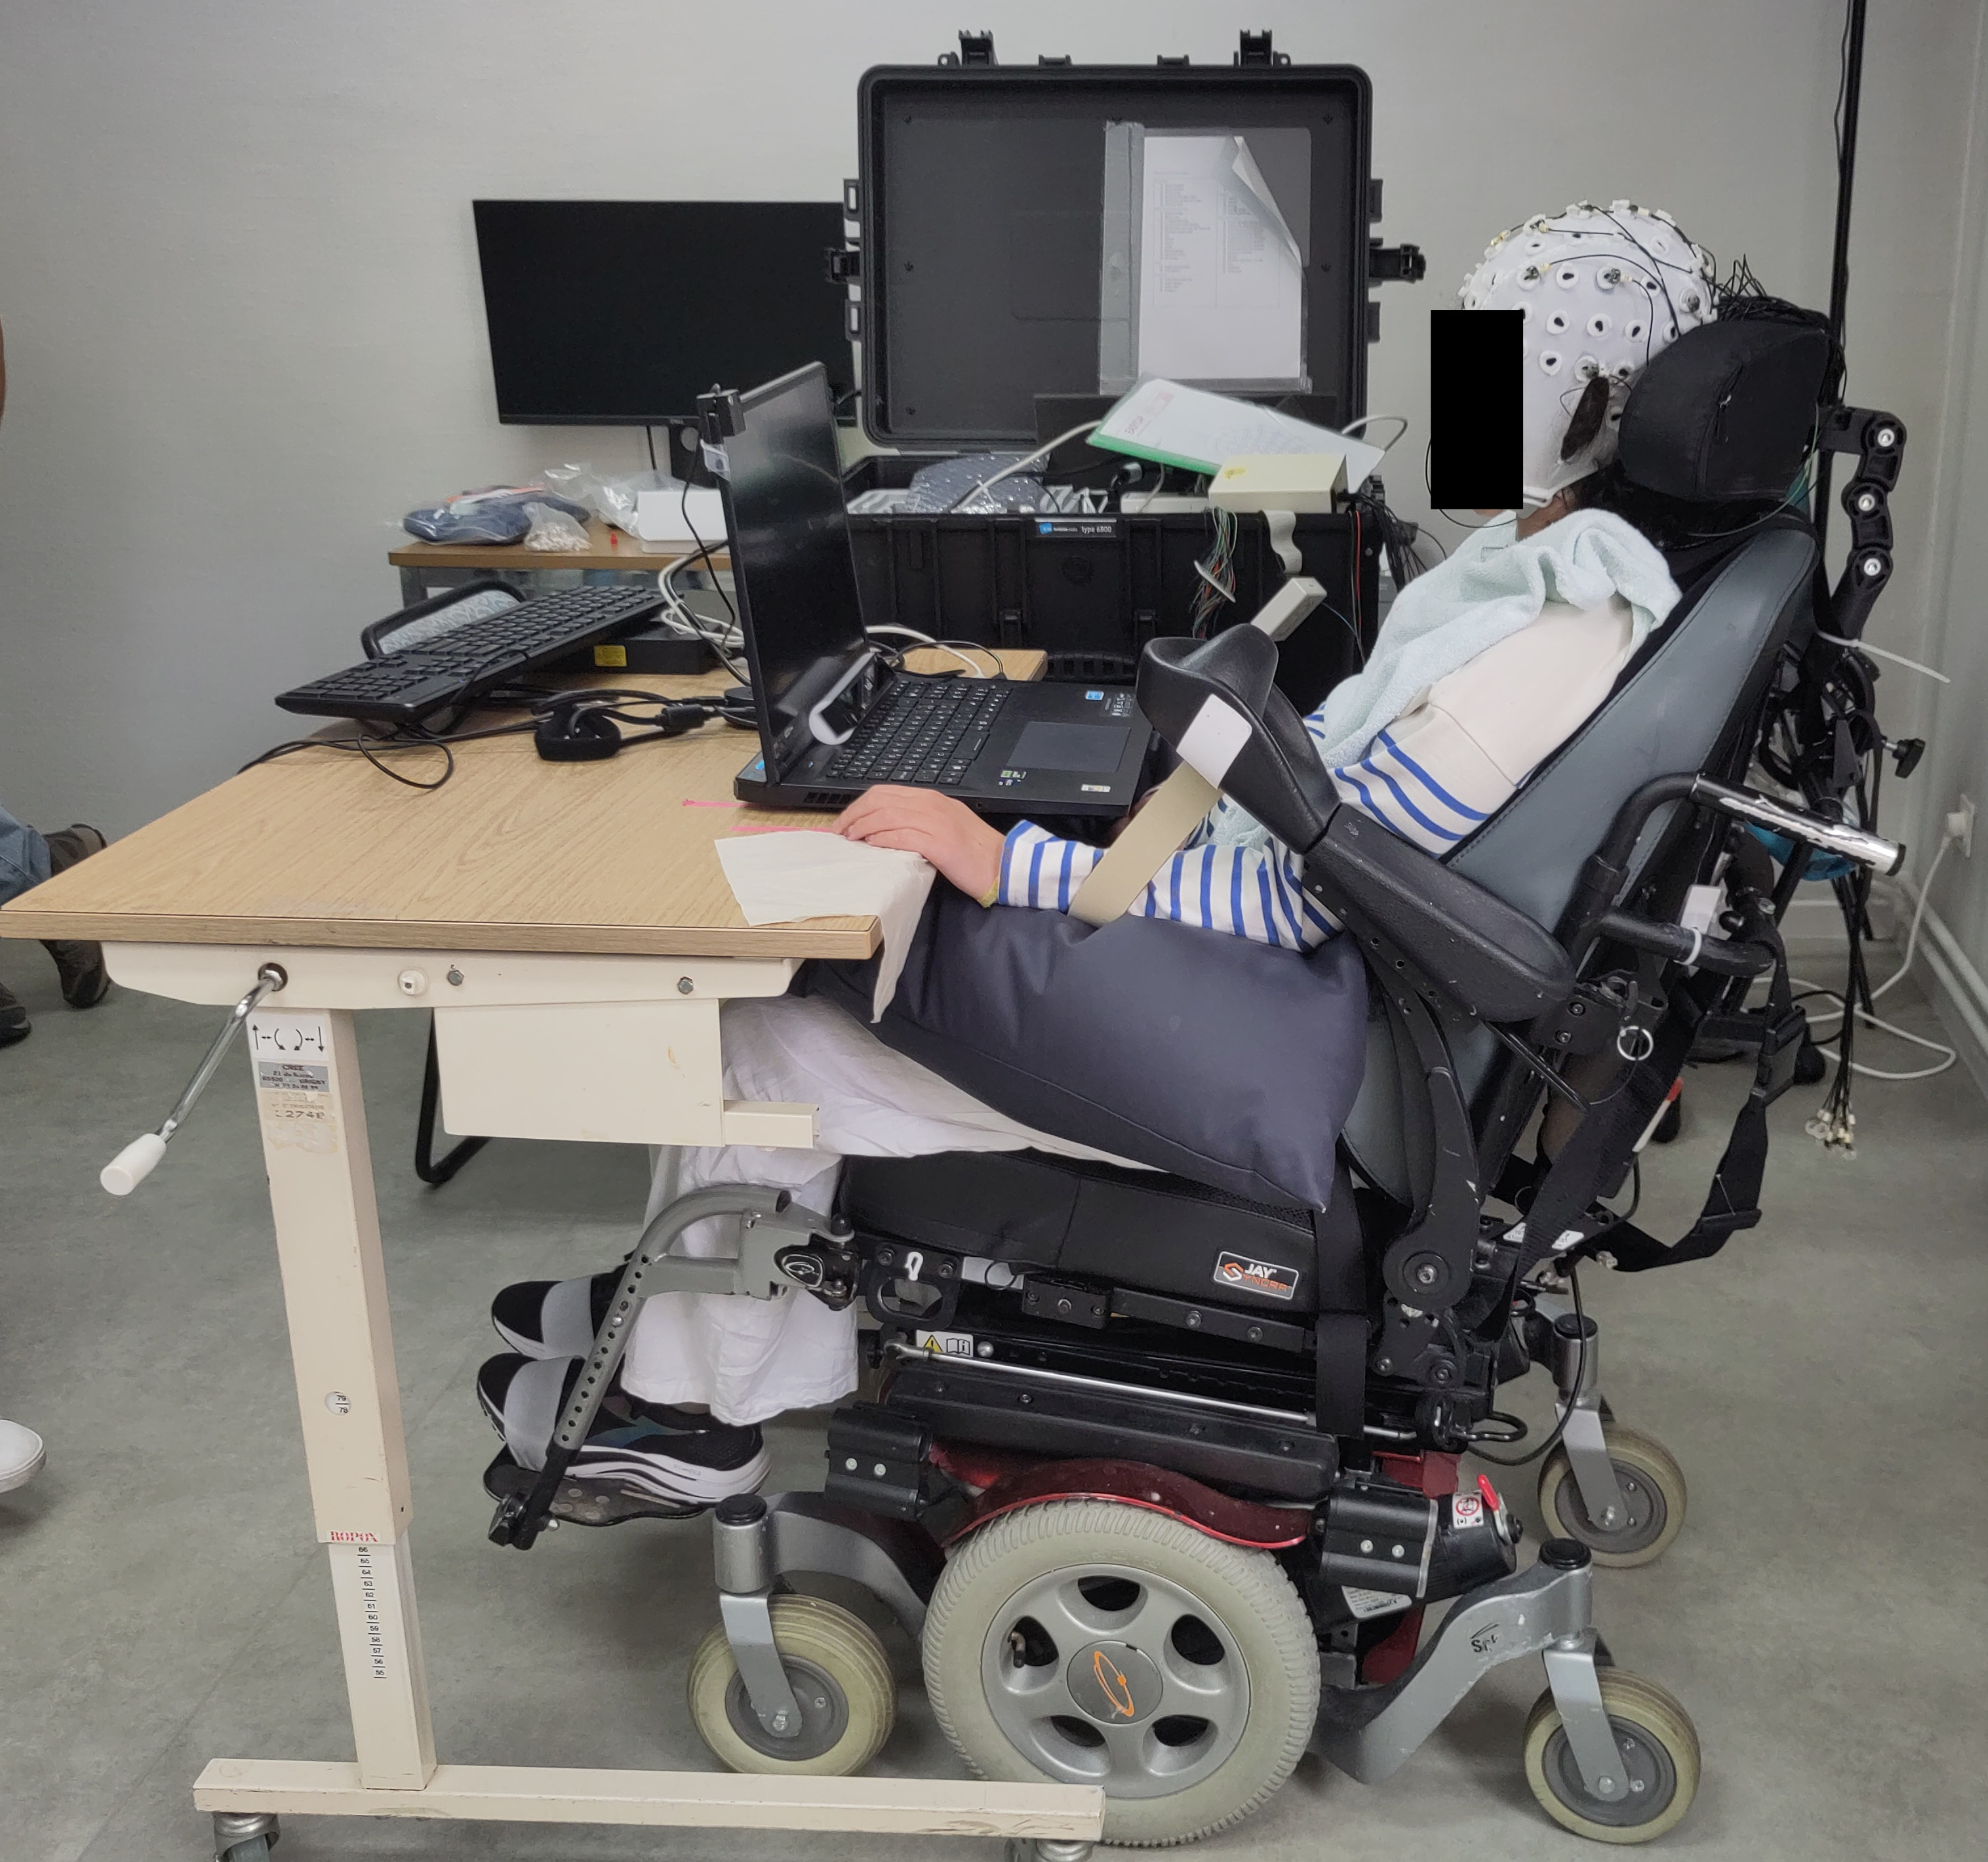
\includegraphics[width=\textwidth]{figures/patients/PD01a-obfuscated.jpg}
  \end{minipage}\hfill%
  \begin{minipage}{.45\textwidth}
    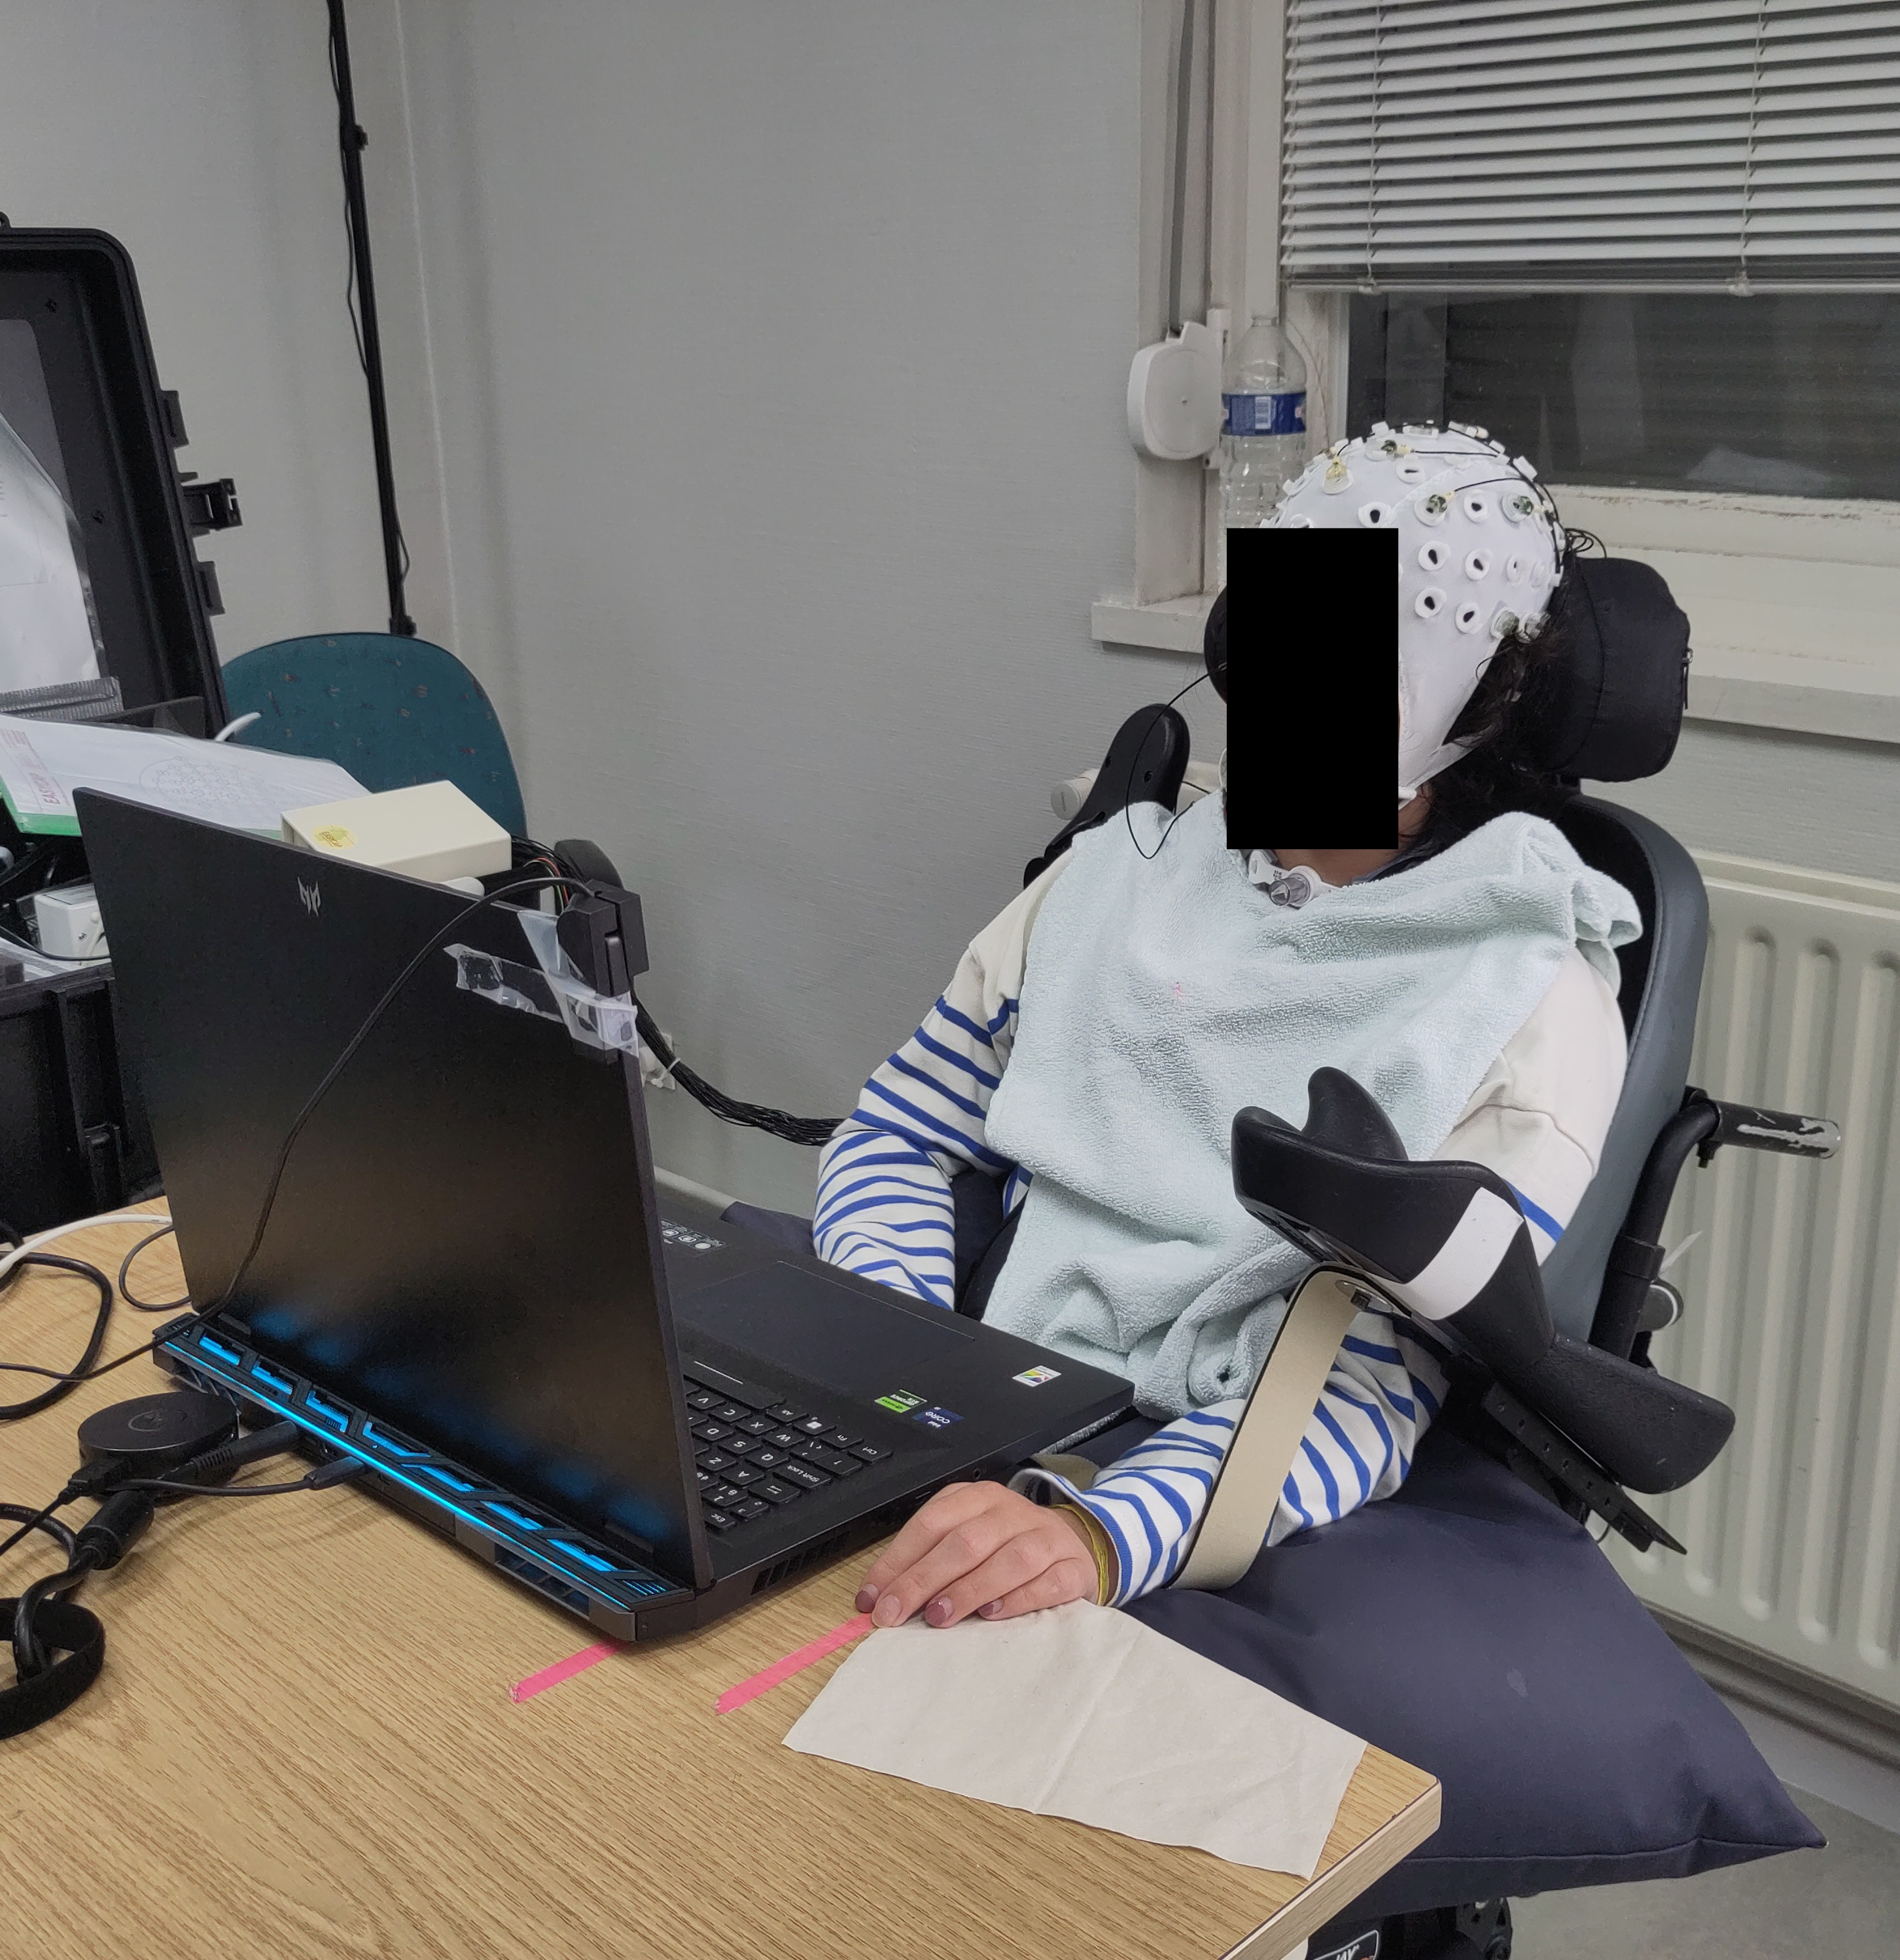
\includegraphics[width=\textwidth]{figures/patients/PD01b-obfuscated.jpg}
  \end{minipage}
  \caption{A participant with the stimulation and recording setup.}
\end{figure}

\subsection{Data collection \& preprocessing}

During the recording session, participants were positioned in their wheelchair in front of a table.
Stimuli were presented on an Acer Predator Helios laptop with an 18" screen (Acer,
Inc., Taiwan) placed at a 60 cm distance.
A Cedrus StimTracker (Cedrus Corp., CA, USA) ensured synchronization of stimuli with the
recorded \ac{eeg}.
Eye tracking was performed throughout using the Tobii X2-30 Compact (Tobii
Technology AB, Sweden) portable eye tracker placed at the bottom of the laptop screen.

\Ac{eeg} was recorded at 1000 Hz using the Neuroscan Neuvo portable amplifier (Compumedics Neuroscan,
Australia) connected to a second laptop for registration.
The \ac{eeg} headset used 18 active AgCl electrodes (EASYCAP GmbH, Germany) placed on a cap
according to the international 10-20 layout.
Using electrolyte gel, electrode impedances were reduced below 10 k$\Omega$.
Additionally, the \ac{eog} was recorded.

The \ac{eeg} was band-pass filtered between 0.5 and 16 Hz.
Bad channels were rejected using the RANSAC algorithm~\cite{Fischler1981}
and visual inspection.
Next, the \ac{eeg} was re-referenced to the average of mastoid electrodes TP9
and TP10, and \ac{ica} was performed to reject artifactual components based on
correlation with the \ac{eog} or by visual inspection.
Epochs were cut from -0.1 to 0.9 s relative to stimulus onset, and no baseline
correction was performed in order to meet the assumptions.

Eye tracking data was cleaned by fusing left and right gaze into one channel
for the horizontal and vertical gaze position.
If both were present for a given sample, the fused channel was the mean of both
values.
If at a given sample either the left or the right eye was not detected for a
given channel, the value of the other one was adopted.
If both were missing, the gaze position remained unset at that time point, and no
interpolation was performed of the employed classifiers.

\subsection{\Acs{bci} decoding}

We evaluated the recorded data using the \ac{wcble}~\cite{VanDenKerchove2024}
and \ac{tlda}~\cite{Sosulski2022}
classifiers, as well as the Riemannian XDAWNCov+TS+LDA~\cite{Cecotti2017}.
For \ac{wcble}, a region of interest from 0 ms to 800 ms relative to stimulus
onset was used while the epoch was cropped to -100 ms to 900 ms. For the other
decoders, the epoch was cropped between 0 ms and 800 ms, which resulted in maximal
performance.
Decoding scores were obtained using 6-fold cross-validation where folds corresponded to
stimulation blocks.

\section{Results}



\subsection{Visual skill and eye tracking analysis}
\label{sec:patients/outcomes/gaze}

Table~\ref{tab:patients/eye} details the eye motor impairments and vision of
the included participants.
All participants reported some degree of fatigue or discomfort when fixating.
Participant PA1 had the mildest impairment, only reporting fatigue when fixating
for prolonged times.
The \ac{fa} participants were mostly affected by eye tremors and impaired pursuit.
PB2 suffered from especially severe horizontal oscillating involuntary eye
movements.
Eye motor function of participants PC2, PC3, and PC4 was most severely affected.
Participant PC2 was only able to look up and down and had a deviation in the
left eye causing diplopia, but this was corrected by a prism glass.
Participant PC3 only retained partial motility of the right eye, while the left eye was permanently closed.
Participant PC4 had one deviated eye with a corneal abscess affecting the motility
and vision in the right eye, and reducing motility in the left.


Given these information, we aimed to shed more light on the actual capabilities of individuals
with \ac{sspgi} regarding performing overt \ac{vsa} and central gaze
fixation, as well as to investigate how relevant these two settings are when the
gaze is not cued.
\Cref{fig:patients/gaze} maps gaze position relative to the stimuli
across conditions.
These results should be interpreted with care, as the eye tracker to some
degree relies on functioning eye motility.
The participant's position relative to the eye tracker might have shifted
throughout the experimental session despite our best efforts, e.g., because they needed aspiration of their
tracheostomy.

\fullpagefig{%
  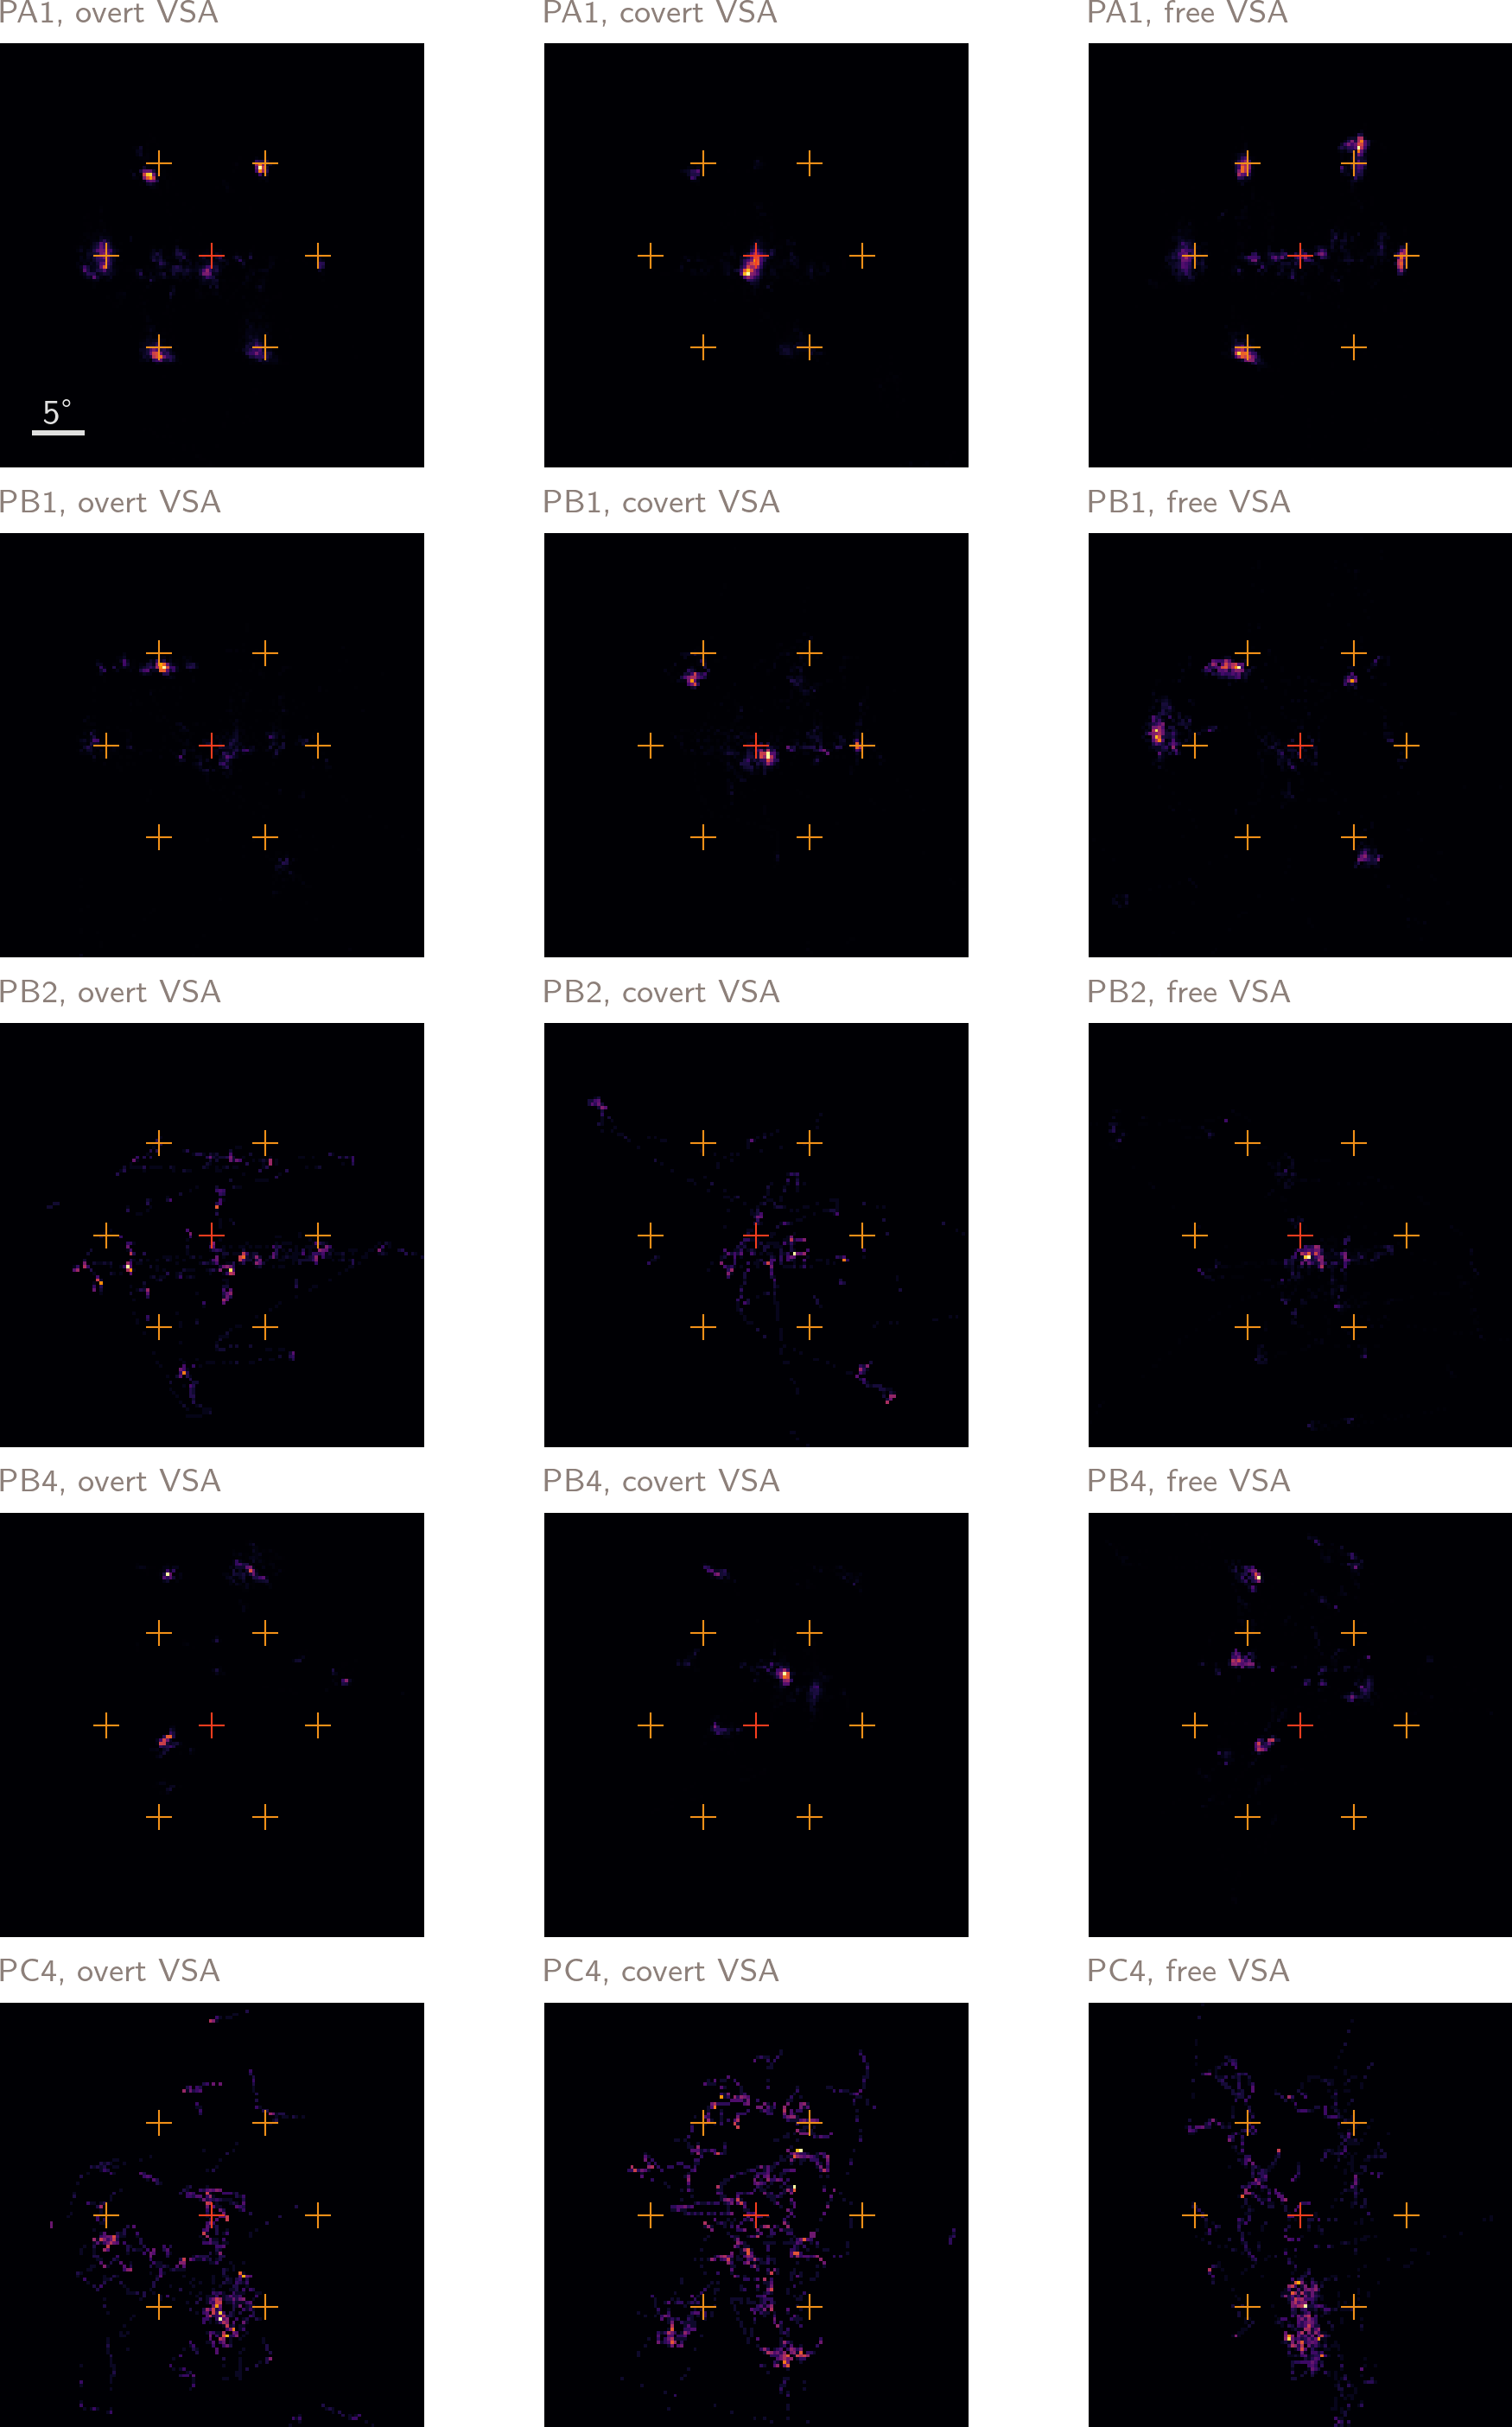
\includegraphics[width=\textwidth]{figures/patients/fig_gaze.png}
}{%
  \caption[Distribution of the recorded gaze position.]{%
    Distribution of the recorded gaze position during the experimental session in the three \ac{vsa}
    conditions.
    Crosshairs represent stimulus positions, with the orange ones cued during
    the given condition.
    Subjects PB2 and PC4 preferred covert \ac{bci} operation, with PB2 resting gaze
    near the middle of the screen, and PC4 near the bottom.
  }
  \label{fig:patients/gaze}
}

PA1 had relatively intact gaze control and was able to correctly perform the
cued overt and covert settings.
When gaze was uncued, he fixated on the cued target.
This was also mostly the case for PB1, although eye tracking revealed that he
chose not to perform central gaze fixation when cued in at least one of the
stimulation blocks. We were unable to record his gaze near the bottom-left
stimulus position, either due to eye tracker failure or because the participant
was not comfortable fixating on this position.
Eye tracker calibration did not succeed for subject PB4, but given
transformation of gaze positions to the stimulus space, they were assumed to
be overtly performing the free task.

PB2 was able to perform overt \ac{vsa} and central fixation to some extent,
yet eye tracking shows a larger spread in gaze position compared to
PA1 and PB1.
In the free \ac{vsa} condition, however, she preferred to attend
stimuli covertly when the gaze was uncued.
This was confirmed by the participant.

The overt and central gaze fixation settings were also not properly adapted to
participant PC4.
In the free \ac{vsa} condition, eye tracker results show that his gaze was usually near the
bottom two targets, indicating some degree of covert or split \ac{vsa}.

It was technically impossible to register gaze position with the Tobii X2-30
Compact for participants PC2 and PC3 since they both had one eye that was
occluded respectively by the prism glass and the eyelid.
Both participants reported they could not fixate on some of the
stimuli.

\subsection{\Acs{bci} decoding performance}

\Cref{fig:patients/decode} shows single-trial
\ac{rocauc} in the evaluated \ac{vsa} settings for the different decoders.


In the overt \ac{vsa} setting, the evaluated decoders performed similarly on average
(\ac{wcble} 75.58\%, XDAWNCov+TS+LDA 74.24\%, \ac{tlda} 75.99\%).
In the covert \ac{vsa} setting with cued central gaze fixation, performance deteriorated,
but \ac{wcble} significantly improved performance over the base classifier
\ac{tlda} in this condition
(\ac{wcble} 62.49\%, XDAWNCov+TS+LDA 59.42\%, \ac{tlda} 59.05\%).
Decoding performance for this task was at chance level for participants PB4 and
PC3.

However, \ac{wcble} did not improve \ac{tlda} performance in the free \ac{vsa} setting, but
XDAWNCov+TS+LDA performance was slightly lower here (though not
significantly).
(\ac{wcble} 74.15\%, XDAWNCov+TS+LDA 71.88\%, \ac{tlda} 74.27\%).
More interestingly, we noticed that performances of the decoders in free
\ac{vsa} were close to those in the overt \ac{vsa}.
A substantial decrease in performance from the overt setting to the free
setting was observed for subjects PC3
(\ac{wcble}: $70.31\%>62.14\%$, XDAWNCov+TS+LDA: $65.78\%>62.18\%$, \ac{tlda}:
$70.49\%>63.76\%$)
and PC4
(\ac{wcble}: $65.56\%>55.71\%$, XDAWNCov+TS+LDA: $62.02\%>54.24\%$, \ac{tlda}:
$66.12\%>57.08\%$).
For PB2, who also relied on covert \ac{vsa} during the uncued free \ac{vsa}
according to gaze tracking setting, the decrease in performance was also
present, but not as substantial
(\ac{wcble}: $82.76\%>78.88\%$, XDAWNCov+TS+LDA: $80.74\%>77.99\%$, \ac{tlda}:
$83.21\%>78.84\%$).

\begin{figure}
  \hspace{-0.16816613518892673in}
%% Creator: Matplotlib, PGF backend
%%
%% To include the figure in your LaTeX document, write
%%   \input{<filename>.pgf}
%%
%% Make sure the required packages are loaded in your preamble
%%   \usepackage{pgf}
%%
%% Also ensure that all the required font packages are loaded; for instance,
%% the lmodern package is sometimes necessary when using math font.
%%   \usepackage{lmodern}
%%
%% Figures using additional raster images can only be included by \input if
%% they are in the same directory as the main LaTeX file. For loading figures
%% from other directories you can use the `import` package
%%   \usepackage{import}
%%
%% and then include the figures with
%%   \import{<path to file>}{<filename>.pgf}
%%
%% Matplotlib used the following preamble
%%
\begingroup%
\makeatletter%
\begin{pgfpicture}%
\pgfpathrectangle{\pgfpointorigin}{\pgfqpoint{4.941931in}{2.000000in}}%
\pgfusepath{use as bounding box, clip}%
\begin{pgfscope}%
\pgfsetbuttcap%
\pgfsetmiterjoin%
\definecolor{currentfill}{rgb}{1.000000,1.000000,1.000000}%
\pgfsetfillcolor{currentfill}%
\pgfsetlinewidth{0.000000pt}%
\definecolor{currentstroke}{rgb}{1.000000,1.000000,1.000000}%
\pgfsetstrokecolor{currentstroke}%
\pgfsetdash{}{0pt}%
\pgfpathmoveto{\pgfqpoint{0.000000in}{0.000000in}}%
\pgfpathlineto{\pgfqpoint{4.941931in}{0.000000in}}%
\pgfpathlineto{\pgfqpoint{4.941931in}{2.000000in}}%
\pgfpathlineto{\pgfqpoint{0.000000in}{2.000000in}}%
\pgfpathlineto{\pgfqpoint{0.000000in}{0.000000in}}%
\pgfpathclose%
\pgfusepath{fill}%
\end{pgfscope}%
\begin{pgfscope}%
\pgfsetbuttcap%
\pgfsetmiterjoin%
\definecolor{currentfill}{rgb}{1.000000,1.000000,1.000000}%
\pgfsetfillcolor{currentfill}%
\pgfsetlinewidth{0.000000pt}%
\definecolor{currentstroke}{rgb}{0.000000,0.000000,0.000000}%
\pgfsetstrokecolor{currentstroke}%
\pgfsetstrokeopacity{0.000000}%
\pgfsetdash{}{0pt}%
\pgfpathmoveto{\pgfqpoint{0.174090in}{0.190223in}}%
\pgfpathlineto{\pgfqpoint{1.713951in}{0.190223in}}%
\pgfpathlineto{\pgfqpoint{1.713951in}{1.872074in}}%
\pgfpathlineto{\pgfqpoint{0.174090in}{1.872074in}}%
\pgfpathlineto{\pgfqpoint{0.174090in}{0.190223in}}%
\pgfpathclose%
\pgfusepath{fill}%
\end{pgfscope}%
\begin{pgfscope}%
\pgfpathrectangle{\pgfqpoint{0.174090in}{0.190223in}}{\pgfqpoint{1.539861in}{1.681851in}}%
\pgfusepath{clip}%
\pgfsetbuttcap%
\pgfsetmiterjoin%
\definecolor{currentfill}{rgb}{0.842157,0.553922,0.200980}%
\pgfsetfillcolor{currentfill}%
\pgfsetlinewidth{0.000000pt}%
\definecolor{currentstroke}{rgb}{0.000000,0.000000,0.000000}%
\pgfsetstrokecolor{currentstroke}%
\pgfsetstrokeopacity{0.000000}%
\pgfsetdash{}{0pt}%
\pgfpathmoveto{\pgfqpoint{0.193338in}{0.190223in}}%
\pgfpathlineto{\pgfqpoint{0.244667in}{0.190223in}}%
\pgfpathlineto{\pgfqpoint{0.244667in}{1.317977in}}%
\pgfpathlineto{\pgfqpoint{0.193338in}{1.317977in}}%
\pgfpathlineto{\pgfqpoint{0.193338in}{0.190223in}}%
\pgfpathclose%
\pgfusepath{fill}%
\end{pgfscope}%
\begin{pgfscope}%
\pgfpathrectangle{\pgfqpoint{0.174090in}{0.190223in}}{\pgfqpoint{1.539861in}{1.681851in}}%
\pgfusepath{clip}%
\pgfsetbuttcap%
\pgfsetmiterjoin%
\definecolor{currentfill}{rgb}{0.842157,0.553922,0.200980}%
\pgfsetfillcolor{currentfill}%
\pgfsetlinewidth{0.000000pt}%
\definecolor{currentstroke}{rgb}{0.000000,0.000000,0.000000}%
\pgfsetstrokecolor{currentstroke}%
\pgfsetstrokeopacity{0.000000}%
\pgfsetdash{}{0pt}%
\pgfpathmoveto{\pgfqpoint{0.385821in}{0.190223in}}%
\pgfpathlineto{\pgfqpoint{0.437150in}{0.190223in}}%
\pgfpathlineto{\pgfqpoint{0.437150in}{1.717496in}}%
\pgfpathlineto{\pgfqpoint{0.385821in}{1.717496in}}%
\pgfpathlineto{\pgfqpoint{0.385821in}{0.190223in}}%
\pgfpathclose%
\pgfusepath{fill}%
\end{pgfscope}%
\begin{pgfscope}%
\pgfpathrectangle{\pgfqpoint{0.174090in}{0.190223in}}{\pgfqpoint{1.539861in}{1.681851in}}%
\pgfusepath{clip}%
\pgfsetbuttcap%
\pgfsetmiterjoin%
\definecolor{currentfill}{rgb}{0.842157,0.553922,0.200980}%
\pgfsetfillcolor{currentfill}%
\pgfsetlinewidth{0.000000pt}%
\definecolor{currentstroke}{rgb}{0.000000,0.000000,0.000000}%
\pgfsetstrokecolor{currentstroke}%
\pgfsetstrokeopacity{0.000000}%
\pgfsetdash{}{0pt}%
\pgfpathmoveto{\pgfqpoint{0.578304in}{0.190223in}}%
\pgfpathlineto{\pgfqpoint{0.629632in}{0.190223in}}%
\pgfpathlineto{\pgfqpoint{0.629632in}{1.589719in}}%
\pgfpathlineto{\pgfqpoint{0.578304in}{1.589719in}}%
\pgfpathlineto{\pgfqpoint{0.578304in}{0.190223in}}%
\pgfpathclose%
\pgfusepath{fill}%
\end{pgfscope}%
\begin{pgfscope}%
\pgfpathrectangle{\pgfqpoint{0.174090in}{0.190223in}}{\pgfqpoint{1.539861in}{1.681851in}}%
\pgfusepath{clip}%
\pgfsetbuttcap%
\pgfsetmiterjoin%
\definecolor{currentfill}{rgb}{0.842157,0.553922,0.200980}%
\pgfsetfillcolor{currentfill}%
\pgfsetlinewidth{0.000000pt}%
\definecolor{currentstroke}{rgb}{0.000000,0.000000,0.000000}%
\pgfsetstrokecolor{currentstroke}%
\pgfsetstrokeopacity{0.000000}%
\pgfsetdash{}{0pt}%
\pgfpathmoveto{\pgfqpoint{0.770786in}{0.190223in}}%
\pgfpathlineto{\pgfqpoint{0.822115in}{0.190223in}}%
\pgfpathlineto{\pgfqpoint{0.822115in}{1.589345in}}%
\pgfpathlineto{\pgfqpoint{0.770786in}{1.589345in}}%
\pgfpathlineto{\pgfqpoint{0.770786in}{0.190223in}}%
\pgfpathclose%
\pgfusepath{fill}%
\end{pgfscope}%
\begin{pgfscope}%
\pgfpathrectangle{\pgfqpoint{0.174090in}{0.190223in}}{\pgfqpoint{1.539861in}{1.681851in}}%
\pgfusepath{clip}%
\pgfsetbuttcap%
\pgfsetmiterjoin%
\definecolor{currentfill}{rgb}{0.842157,0.553922,0.200980}%
\pgfsetfillcolor{currentfill}%
\pgfsetlinewidth{0.000000pt}%
\definecolor{currentstroke}{rgb}{0.000000,0.000000,0.000000}%
\pgfsetstrokecolor{currentstroke}%
\pgfsetstrokeopacity{0.000000}%
\pgfsetdash{}{0pt}%
\pgfpathmoveto{\pgfqpoint{0.963269in}{0.190223in}}%
\pgfpathlineto{\pgfqpoint{1.014598in}{0.190223in}}%
\pgfpathlineto{\pgfqpoint{1.014598in}{1.384946in}}%
\pgfpathlineto{\pgfqpoint{0.963269in}{1.384946in}}%
\pgfpathlineto{\pgfqpoint{0.963269in}{0.190223in}}%
\pgfpathclose%
\pgfusepath{fill}%
\end{pgfscope}%
\begin{pgfscope}%
\pgfpathrectangle{\pgfqpoint{0.174090in}{0.190223in}}{\pgfqpoint{1.539861in}{1.681851in}}%
\pgfusepath{clip}%
\pgfsetbuttcap%
\pgfsetmiterjoin%
\definecolor{currentfill}{rgb}{0.842157,0.553922,0.200980}%
\pgfsetfillcolor{currentfill}%
\pgfsetlinewidth{0.000000pt}%
\definecolor{currentstroke}{rgb}{0.000000,0.000000,0.000000}%
\pgfsetstrokecolor{currentstroke}%
\pgfsetstrokeopacity{0.000000}%
\pgfsetdash{}{0pt}%
\pgfpathmoveto{\pgfqpoint{1.155752in}{0.190223in}}%
\pgfpathlineto{\pgfqpoint{1.207080in}{0.190223in}}%
\pgfpathlineto{\pgfqpoint{1.207080in}{1.375840in}}%
\pgfpathlineto{\pgfqpoint{1.155752in}{1.375840in}}%
\pgfpathlineto{\pgfqpoint{1.155752in}{0.190223in}}%
\pgfpathclose%
\pgfusepath{fill}%
\end{pgfscope}%
\begin{pgfscope}%
\pgfpathrectangle{\pgfqpoint{0.174090in}{0.190223in}}{\pgfqpoint{1.539861in}{1.681851in}}%
\pgfusepath{clip}%
\pgfsetbuttcap%
\pgfsetmiterjoin%
\definecolor{currentfill}{rgb}{0.842157,0.553922,0.200980}%
\pgfsetfillcolor{currentfill}%
\pgfsetlinewidth{0.000000pt}%
\definecolor{currentstroke}{rgb}{0.000000,0.000000,0.000000}%
\pgfsetstrokecolor{currentstroke}%
\pgfsetstrokeopacity{0.000000}%
\pgfsetdash{}{0pt}%
\pgfpathmoveto{\pgfqpoint{1.348234in}{0.190223in}}%
\pgfpathlineto{\pgfqpoint{1.399563in}{0.190223in}}%
\pgfpathlineto{\pgfqpoint{1.399563in}{1.302232in}}%
\pgfpathlineto{\pgfqpoint{1.348234in}{1.302232in}}%
\pgfpathlineto{\pgfqpoint{1.348234in}{0.190223in}}%
\pgfpathclose%
\pgfusepath{fill}%
\end{pgfscope}%
\begin{pgfscope}%
\pgfpathrectangle{\pgfqpoint{0.174090in}{0.190223in}}{\pgfqpoint{1.539861in}{1.681851in}}%
\pgfusepath{clip}%
\pgfsetbuttcap%
\pgfsetmiterjoin%
\definecolor{currentfill}{rgb}{0.842157,0.553922,0.200980}%
\pgfsetfillcolor{currentfill}%
\pgfsetlinewidth{0.000000pt}%
\definecolor{currentstroke}{rgb}{0.000000,0.000000,0.000000}%
\pgfsetstrokecolor{currentstroke}%
\pgfsetstrokeopacity{0.000000}%
\pgfsetdash{}{0pt}%
\pgfpathmoveto{\pgfqpoint{1.540717in}{0.190223in}}%
\pgfpathlineto{\pgfqpoint{1.592046in}{0.190223in}}%
\pgfpathlineto{\pgfqpoint{1.592046in}{1.468222in}}%
\pgfpathlineto{\pgfqpoint{1.540717in}{1.468222in}}%
\pgfpathlineto{\pgfqpoint{1.540717in}{0.190223in}}%
\pgfpathclose%
\pgfusepath{fill}%
\end{pgfscope}%
\begin{pgfscope}%
\pgfpathrectangle{\pgfqpoint{0.174090in}{0.190223in}}{\pgfqpoint{1.539861in}{1.681851in}}%
\pgfusepath{clip}%
\pgfsetbuttcap%
\pgfsetmiterjoin%
\definecolor{currentfill}{rgb}{0.858824,0.314706,0.223529}%
\pgfsetfillcolor{currentfill}%
\pgfsetlinewidth{0.000000pt}%
\definecolor{currentstroke}{rgb}{0.000000,0.000000,0.000000}%
\pgfsetstrokecolor{currentstroke}%
\pgfsetstrokeopacity{0.000000}%
\pgfsetdash{}{0pt}%
\pgfpathmoveto{\pgfqpoint{0.244667in}{0.190223in}}%
\pgfpathlineto{\pgfqpoint{0.295996in}{0.190223in}}%
\pgfpathlineto{\pgfqpoint{0.295996in}{1.393596in}}%
\pgfpathlineto{\pgfqpoint{0.244667in}{1.393596in}}%
\pgfpathlineto{\pgfqpoint{0.244667in}{0.190223in}}%
\pgfpathclose%
\pgfusepath{fill}%
\end{pgfscope}%
\begin{pgfscope}%
\pgfpathrectangle{\pgfqpoint{0.174090in}{0.190223in}}{\pgfqpoint{1.539861in}{1.681851in}}%
\pgfusepath{clip}%
\pgfsetbuttcap%
\pgfsetmiterjoin%
\definecolor{currentfill}{rgb}{0.858824,0.314706,0.223529}%
\pgfsetfillcolor{currentfill}%
\pgfsetlinewidth{0.000000pt}%
\definecolor{currentstroke}{rgb}{0.000000,0.000000,0.000000}%
\pgfsetstrokecolor{currentstroke}%
\pgfsetstrokeopacity{0.000000}%
\pgfsetdash{}{0pt}%
\pgfpathmoveto{\pgfqpoint{0.437150in}{0.190223in}}%
\pgfpathlineto{\pgfqpoint{0.488478in}{0.190223in}}%
\pgfpathlineto{\pgfqpoint{0.488478in}{1.695290in}}%
\pgfpathlineto{\pgfqpoint{0.437150in}{1.695290in}}%
\pgfpathlineto{\pgfqpoint{0.437150in}{0.190223in}}%
\pgfpathclose%
\pgfusepath{fill}%
\end{pgfscope}%
\begin{pgfscope}%
\pgfpathrectangle{\pgfqpoint{0.174090in}{0.190223in}}{\pgfqpoint{1.539861in}{1.681851in}}%
\pgfusepath{clip}%
\pgfsetbuttcap%
\pgfsetmiterjoin%
\definecolor{currentfill}{rgb}{0.858824,0.314706,0.223529}%
\pgfsetfillcolor{currentfill}%
\pgfsetlinewidth{0.000000pt}%
\definecolor{currentstroke}{rgb}{0.000000,0.000000,0.000000}%
\pgfsetstrokecolor{currentstroke}%
\pgfsetstrokeopacity{0.000000}%
\pgfsetdash{}{0pt}%
\pgfpathmoveto{\pgfqpoint{0.629632in}{0.190223in}}%
\pgfpathlineto{\pgfqpoint{0.680961in}{0.190223in}}%
\pgfpathlineto{\pgfqpoint{0.680961in}{1.582085in}}%
\pgfpathlineto{\pgfqpoint{0.629632in}{1.582085in}}%
\pgfpathlineto{\pgfqpoint{0.629632in}{0.190223in}}%
\pgfpathclose%
\pgfusepath{fill}%
\end{pgfscope}%
\begin{pgfscope}%
\pgfpathrectangle{\pgfqpoint{0.174090in}{0.190223in}}{\pgfqpoint{1.539861in}{1.681851in}}%
\pgfusepath{clip}%
\pgfsetbuttcap%
\pgfsetmiterjoin%
\definecolor{currentfill}{rgb}{0.858824,0.314706,0.223529}%
\pgfsetfillcolor{currentfill}%
\pgfsetlinewidth{0.000000pt}%
\definecolor{currentstroke}{rgb}{0.000000,0.000000,0.000000}%
\pgfsetstrokecolor{currentstroke}%
\pgfsetstrokeopacity{0.000000}%
\pgfsetdash{}{0pt}%
\pgfpathmoveto{\pgfqpoint{0.822115in}{0.190223in}}%
\pgfpathlineto{\pgfqpoint{0.873444in}{0.190223in}}%
\pgfpathlineto{\pgfqpoint{0.873444in}{1.544680in}}%
\pgfpathlineto{\pgfqpoint{0.822115in}{1.544680in}}%
\pgfpathlineto{\pgfqpoint{0.822115in}{0.190223in}}%
\pgfpathclose%
\pgfusepath{fill}%
\end{pgfscope}%
\begin{pgfscope}%
\pgfpathrectangle{\pgfqpoint{0.174090in}{0.190223in}}{\pgfqpoint{1.539861in}{1.681851in}}%
\pgfusepath{clip}%
\pgfsetbuttcap%
\pgfsetmiterjoin%
\definecolor{currentfill}{rgb}{0.858824,0.314706,0.223529}%
\pgfsetfillcolor{currentfill}%
\pgfsetlinewidth{0.000000pt}%
\definecolor{currentstroke}{rgb}{0.000000,0.000000,0.000000}%
\pgfsetstrokecolor{currentstroke}%
\pgfsetstrokeopacity{0.000000}%
\pgfsetdash{}{0pt}%
\pgfpathmoveto{\pgfqpoint{1.014598in}{0.190223in}}%
\pgfpathlineto{\pgfqpoint{1.065926in}{0.190223in}}%
\pgfpathlineto{\pgfqpoint{1.065926in}{1.346833in}}%
\pgfpathlineto{\pgfqpoint{1.014598in}{1.346833in}}%
\pgfpathlineto{\pgfqpoint{1.014598in}{0.190223in}}%
\pgfpathclose%
\pgfusepath{fill}%
\end{pgfscope}%
\begin{pgfscope}%
\pgfpathrectangle{\pgfqpoint{0.174090in}{0.190223in}}{\pgfqpoint{1.539861in}{1.681851in}}%
\pgfusepath{clip}%
\pgfsetbuttcap%
\pgfsetmiterjoin%
\definecolor{currentfill}{rgb}{0.858824,0.314706,0.223529}%
\pgfsetfillcolor{currentfill}%
\pgfsetlinewidth{0.000000pt}%
\definecolor{currentstroke}{rgb}{0.000000,0.000000,0.000000}%
\pgfsetstrokecolor{currentstroke}%
\pgfsetstrokeopacity{0.000000}%
\pgfsetdash{}{0pt}%
\pgfpathmoveto{\pgfqpoint{1.207080in}{0.190223in}}%
\pgfpathlineto{\pgfqpoint{1.258409in}{0.190223in}}%
\pgfpathlineto{\pgfqpoint{1.258409in}{1.372747in}}%
\pgfpathlineto{\pgfqpoint{1.207080in}{1.372747in}}%
\pgfpathlineto{\pgfqpoint{1.207080in}{0.190223in}}%
\pgfpathclose%
\pgfusepath{fill}%
\end{pgfscope}%
\begin{pgfscope}%
\pgfpathrectangle{\pgfqpoint{0.174090in}{0.190223in}}{\pgfqpoint{1.539861in}{1.681851in}}%
\pgfusepath{clip}%
\pgfsetbuttcap%
\pgfsetmiterjoin%
\definecolor{currentfill}{rgb}{0.858824,0.314706,0.223529}%
\pgfsetfillcolor{currentfill}%
\pgfsetlinewidth{0.000000pt}%
\definecolor{currentstroke}{rgb}{0.000000,0.000000,0.000000}%
\pgfsetstrokecolor{currentstroke}%
\pgfsetstrokeopacity{0.000000}%
\pgfsetdash{}{0pt}%
\pgfpathmoveto{\pgfqpoint{1.399563in}{0.190223in}}%
\pgfpathlineto{\pgfqpoint{1.450892in}{0.190223in}}%
\pgfpathlineto{\pgfqpoint{1.450892in}{1.294360in}}%
\pgfpathlineto{\pgfqpoint{1.399563in}{1.294360in}}%
\pgfpathlineto{\pgfqpoint{1.399563in}{0.190223in}}%
\pgfpathclose%
\pgfusepath{fill}%
\end{pgfscope}%
\begin{pgfscope}%
\pgfpathrectangle{\pgfqpoint{0.174090in}{0.190223in}}{\pgfqpoint{1.539861in}{1.681851in}}%
\pgfusepath{clip}%
\pgfsetbuttcap%
\pgfsetmiterjoin%
\definecolor{currentfill}{rgb}{0.858824,0.314706,0.223529}%
\pgfsetfillcolor{currentfill}%
\pgfsetlinewidth{0.000000pt}%
\definecolor{currentstroke}{rgb}{0.000000,0.000000,0.000000}%
\pgfsetstrokecolor{currentstroke}%
\pgfsetstrokeopacity{0.000000}%
\pgfsetdash{}{0pt}%
\pgfpathmoveto{\pgfqpoint{1.592046in}{0.190223in}}%
\pgfpathlineto{\pgfqpoint{1.643374in}{0.190223in}}%
\pgfpathlineto{\pgfqpoint{1.643374in}{1.461370in}}%
\pgfpathlineto{\pgfqpoint{1.592046in}{1.461370in}}%
\pgfpathlineto{\pgfqpoint{1.592046in}{0.190223in}}%
\pgfpathclose%
\pgfusepath{fill}%
\end{pgfscope}%
\begin{pgfscope}%
\pgfpathrectangle{\pgfqpoint{0.174090in}{0.190223in}}{\pgfqpoint{1.539861in}{1.681851in}}%
\pgfusepath{clip}%
\pgfsetbuttcap%
\pgfsetmiterjoin%
\definecolor{currentfill}{rgb}{0.464706,0.320588,0.573529}%
\pgfsetfillcolor{currentfill}%
\pgfsetlinewidth{0.000000pt}%
\definecolor{currentstroke}{rgb}{0.000000,0.000000,0.000000}%
\pgfsetstrokecolor{currentstroke}%
\pgfsetstrokeopacity{0.000000}%
\pgfsetdash{}{0pt}%
\pgfpathmoveto{\pgfqpoint{0.295996in}{0.190223in}}%
\pgfpathlineto{\pgfqpoint{0.347325in}{0.190223in}}%
\pgfpathlineto{\pgfqpoint{0.347325in}{1.332130in}}%
\pgfpathlineto{\pgfqpoint{0.295996in}{1.332130in}}%
\pgfpathlineto{\pgfqpoint{0.295996in}{0.190223in}}%
\pgfpathclose%
\pgfusepath{fill}%
\end{pgfscope}%
\begin{pgfscope}%
\pgfpathrectangle{\pgfqpoint{0.174090in}{0.190223in}}{\pgfqpoint{1.539861in}{1.681851in}}%
\pgfusepath{clip}%
\pgfsetbuttcap%
\pgfsetmiterjoin%
\definecolor{currentfill}{rgb}{0.464706,0.320588,0.573529}%
\pgfsetfillcolor{currentfill}%
\pgfsetlinewidth{0.000000pt}%
\definecolor{currentstroke}{rgb}{0.000000,0.000000,0.000000}%
\pgfsetstrokecolor{currentstroke}%
\pgfsetstrokeopacity{0.000000}%
\pgfsetdash{}{0pt}%
\pgfpathmoveto{\pgfqpoint{0.488478in}{0.190223in}}%
\pgfpathlineto{\pgfqpoint{0.539807in}{0.190223in}}%
\pgfpathlineto{\pgfqpoint{0.539807in}{1.696667in}}%
\pgfpathlineto{\pgfqpoint{0.488478in}{1.696667in}}%
\pgfpathlineto{\pgfqpoint{0.488478in}{0.190223in}}%
\pgfpathclose%
\pgfusepath{fill}%
\end{pgfscope}%
\begin{pgfscope}%
\pgfpathrectangle{\pgfqpoint{0.174090in}{0.190223in}}{\pgfqpoint{1.539861in}{1.681851in}}%
\pgfusepath{clip}%
\pgfsetbuttcap%
\pgfsetmiterjoin%
\definecolor{currentfill}{rgb}{0.464706,0.320588,0.573529}%
\pgfsetfillcolor{currentfill}%
\pgfsetlinewidth{0.000000pt}%
\definecolor{currentstroke}{rgb}{0.000000,0.000000,0.000000}%
\pgfsetstrokecolor{currentstroke}%
\pgfsetstrokeopacity{0.000000}%
\pgfsetdash{}{0pt}%
\pgfpathmoveto{\pgfqpoint{0.680961in}{0.190223in}}%
\pgfpathlineto{\pgfqpoint{0.732290in}{0.190223in}}%
\pgfpathlineto{\pgfqpoint{0.732290in}{1.548223in}}%
\pgfpathlineto{\pgfqpoint{0.680961in}{1.548223in}}%
\pgfpathlineto{\pgfqpoint{0.680961in}{0.190223in}}%
\pgfpathclose%
\pgfusepath{fill}%
\end{pgfscope}%
\begin{pgfscope}%
\pgfpathrectangle{\pgfqpoint{0.174090in}{0.190223in}}{\pgfqpoint{1.539861in}{1.681851in}}%
\pgfusepath{clip}%
\pgfsetbuttcap%
\pgfsetmiterjoin%
\definecolor{currentfill}{rgb}{0.464706,0.320588,0.573529}%
\pgfsetfillcolor{currentfill}%
\pgfsetlinewidth{0.000000pt}%
\definecolor{currentstroke}{rgb}{0.000000,0.000000,0.000000}%
\pgfsetstrokecolor{currentstroke}%
\pgfsetstrokeopacity{0.000000}%
\pgfsetdash{}{0pt}%
\pgfpathmoveto{\pgfqpoint{0.873444in}{0.190223in}}%
\pgfpathlineto{\pgfqpoint{0.924772in}{0.190223in}}%
\pgfpathlineto{\pgfqpoint{0.924772in}{1.582413in}}%
\pgfpathlineto{\pgfqpoint{0.873444in}{1.582413in}}%
\pgfpathlineto{\pgfqpoint{0.873444in}{0.190223in}}%
\pgfpathclose%
\pgfusepath{fill}%
\end{pgfscope}%
\begin{pgfscope}%
\pgfpathrectangle{\pgfqpoint{0.174090in}{0.190223in}}{\pgfqpoint{1.539861in}{1.681851in}}%
\pgfusepath{clip}%
\pgfsetbuttcap%
\pgfsetmiterjoin%
\definecolor{currentfill}{rgb}{0.464706,0.320588,0.573529}%
\pgfsetfillcolor{currentfill}%
\pgfsetlinewidth{0.000000pt}%
\definecolor{currentstroke}{rgb}{0.000000,0.000000,0.000000}%
\pgfsetstrokecolor{currentstroke}%
\pgfsetstrokeopacity{0.000000}%
\pgfsetdash{}{0pt}%
\pgfpathmoveto{\pgfqpoint{1.065926in}{0.190223in}}%
\pgfpathlineto{\pgfqpoint{1.117255in}{0.190223in}}%
\pgfpathlineto{\pgfqpoint{1.117255in}{1.389045in}}%
\pgfpathlineto{\pgfqpoint{1.065926in}{1.389045in}}%
\pgfpathlineto{\pgfqpoint{1.065926in}{0.190223in}}%
\pgfpathclose%
\pgfusepath{fill}%
\end{pgfscope}%
\begin{pgfscope}%
\pgfpathrectangle{\pgfqpoint{0.174090in}{0.190223in}}{\pgfqpoint{1.539861in}{1.681851in}}%
\pgfusepath{clip}%
\pgfsetbuttcap%
\pgfsetmiterjoin%
\definecolor{currentfill}{rgb}{0.464706,0.320588,0.573529}%
\pgfsetfillcolor{currentfill}%
\pgfsetlinewidth{0.000000pt}%
\definecolor{currentstroke}{rgb}{0.000000,0.000000,0.000000}%
\pgfsetstrokecolor{currentstroke}%
\pgfsetstrokeopacity{0.000000}%
\pgfsetdash{}{0pt}%
\pgfpathmoveto{\pgfqpoint{1.258409in}{0.190223in}}%
\pgfpathlineto{\pgfqpoint{1.309738in}{0.190223in}}%
\pgfpathlineto{\pgfqpoint{1.309738in}{1.289552in}}%
\pgfpathlineto{\pgfqpoint{1.258409in}{1.289552in}}%
\pgfpathlineto{\pgfqpoint{1.258409in}{0.190223in}}%
\pgfpathclose%
\pgfusepath{fill}%
\end{pgfscope}%
\begin{pgfscope}%
\pgfpathrectangle{\pgfqpoint{0.174090in}{0.190223in}}{\pgfqpoint{1.539861in}{1.681851in}}%
\pgfusepath{clip}%
\pgfsetbuttcap%
\pgfsetmiterjoin%
\definecolor{currentfill}{rgb}{0.464706,0.320588,0.573529}%
\pgfsetfillcolor{currentfill}%
\pgfsetlinewidth{0.000000pt}%
\definecolor{currentstroke}{rgb}{0.000000,0.000000,0.000000}%
\pgfsetstrokecolor{currentstroke}%
\pgfsetstrokeopacity{0.000000}%
\pgfsetdash{}{0pt}%
\pgfpathmoveto{\pgfqpoint{1.450892in}{0.190223in}}%
\pgfpathlineto{\pgfqpoint{1.502220in}{0.190223in}}%
\pgfpathlineto{\pgfqpoint{1.502220in}{1.233230in}}%
\pgfpathlineto{\pgfqpoint{1.450892in}{1.233230in}}%
\pgfpathlineto{\pgfqpoint{1.450892in}{0.190223in}}%
\pgfpathclose%
\pgfusepath{fill}%
\end{pgfscope}%
\begin{pgfscope}%
\pgfpathrectangle{\pgfqpoint{0.174090in}{0.190223in}}{\pgfqpoint{1.539861in}{1.681851in}}%
\pgfusepath{clip}%
\pgfsetbuttcap%
\pgfsetmiterjoin%
\definecolor{currentfill}{rgb}{0.464706,0.320588,0.573529}%
\pgfsetfillcolor{currentfill}%
\pgfsetlinewidth{0.000000pt}%
\definecolor{currentstroke}{rgb}{0.000000,0.000000,0.000000}%
\pgfsetstrokecolor{currentstroke}%
\pgfsetstrokeopacity{0.000000}%
\pgfsetdash{}{0pt}%
\pgfpathmoveto{\pgfqpoint{1.643374in}{0.190223in}}%
\pgfpathlineto{\pgfqpoint{1.694703in}{0.190223in}}%
\pgfpathlineto{\pgfqpoint{1.694703in}{1.438751in}}%
\pgfpathlineto{\pgfqpoint{1.643374in}{1.438751in}}%
\pgfpathlineto{\pgfqpoint{1.643374in}{0.190223in}}%
\pgfpathclose%
\pgfusepath{fill}%
\end{pgfscope}%
\begin{pgfscope}%
\pgfsetbuttcap%
\pgfsetroundjoin%
\definecolor{currentfill}{rgb}{0.552941,0.501961,0.478431}%
\pgfsetfillcolor{currentfill}%
\pgfsetlinewidth{0.803000pt}%
\definecolor{currentstroke}{rgb}{0.552941,0.501961,0.478431}%
\pgfsetstrokecolor{currentstroke}%
\pgfsetdash{}{0pt}%
\pgfsys@defobject{currentmarker}{\pgfqpoint{0.000000in}{0.000000in}}{\pgfqpoint{0.000000in}{0.041667in}}{%
\pgfpathmoveto{\pgfqpoint{0.000000in}{0.000000in}}%
\pgfpathlineto{\pgfqpoint{0.000000in}{0.041667in}}%
\pgfusepath{stroke,fill}%
}%
\begin{pgfscope}%
\pgfsys@transformshift{0.270331in}{0.190223in}%
\pgfsys@useobject{currentmarker}{}%
\end{pgfscope}%
\end{pgfscope}%
\begin{pgfscope}%
\definecolor{textcolor}{rgb}{0.552941,0.501961,0.478431}%
\pgfsetstrokecolor{textcolor}%
\pgfsetfillcolor{textcolor}%
\pgftext[x=0.301581in, y=-0.079933in, left, base,rotate=90.000000]{\color{textcolor}\sffamily\fontsize{9.000000}{10.800000}\selectfont PA1}%
\end{pgfscope}%
\begin{pgfscope}%
\pgfsetbuttcap%
\pgfsetroundjoin%
\definecolor{currentfill}{rgb}{0.552941,0.501961,0.478431}%
\pgfsetfillcolor{currentfill}%
\pgfsetlinewidth{0.803000pt}%
\definecolor{currentstroke}{rgb}{0.552941,0.501961,0.478431}%
\pgfsetstrokecolor{currentstroke}%
\pgfsetdash{}{0pt}%
\pgfsys@defobject{currentmarker}{\pgfqpoint{0.000000in}{0.000000in}}{\pgfqpoint{0.000000in}{0.041667in}}{%
\pgfpathmoveto{\pgfqpoint{0.000000in}{0.000000in}}%
\pgfpathlineto{\pgfqpoint{0.000000in}{0.041667in}}%
\pgfusepath{stroke,fill}%
}%
\begin{pgfscope}%
\pgfsys@transformshift{0.462814in}{0.190223in}%
\pgfsys@useobject{currentmarker}{}%
\end{pgfscope}%
\end{pgfscope}%
\begin{pgfscope}%
\definecolor{textcolor}{rgb}{0.552941,0.501961,0.478431}%
\pgfsetstrokecolor{textcolor}%
\pgfsetfillcolor{textcolor}%
\pgftext[x=0.494064in, y=-0.090543in, left, base,rotate=90.000000]{\color{textcolor}\sffamily\fontsize{9.000000}{10.800000}\selectfont PB1}%
\end{pgfscope}%
\begin{pgfscope}%
\pgfsetbuttcap%
\pgfsetroundjoin%
\definecolor{currentfill}{rgb}{0.552941,0.501961,0.478431}%
\pgfsetfillcolor{currentfill}%
\pgfsetlinewidth{0.803000pt}%
\definecolor{currentstroke}{rgb}{0.552941,0.501961,0.478431}%
\pgfsetstrokecolor{currentstroke}%
\pgfsetdash{}{0pt}%
\pgfsys@defobject{currentmarker}{\pgfqpoint{0.000000in}{0.000000in}}{\pgfqpoint{0.000000in}{0.041667in}}{%
\pgfpathmoveto{\pgfqpoint{0.000000in}{0.000000in}}%
\pgfpathlineto{\pgfqpoint{0.000000in}{0.041667in}}%
\pgfusepath{stroke,fill}%
}%
\begin{pgfscope}%
\pgfsys@transformshift{0.655297in}{0.190223in}%
\pgfsys@useobject{currentmarker}{}%
\end{pgfscope}%
\end{pgfscope}%
\begin{pgfscope}%
\definecolor{textcolor}{rgb}{0.552941,0.501961,0.478431}%
\pgfsetstrokecolor{textcolor}%
\pgfsetfillcolor{textcolor}%
\pgftext[x=0.686547in, y=-0.090543in, left, base,rotate=90.000000]{\color{textcolor}\sffamily\fontsize{9.000000}{10.800000}\selectfont PB2}%
\end{pgfscope}%
\begin{pgfscope}%
\pgfsetbuttcap%
\pgfsetroundjoin%
\definecolor{currentfill}{rgb}{0.552941,0.501961,0.478431}%
\pgfsetfillcolor{currentfill}%
\pgfsetlinewidth{0.803000pt}%
\definecolor{currentstroke}{rgb}{0.552941,0.501961,0.478431}%
\pgfsetstrokecolor{currentstroke}%
\pgfsetdash{}{0pt}%
\pgfsys@defobject{currentmarker}{\pgfqpoint{0.000000in}{0.000000in}}{\pgfqpoint{0.000000in}{0.041667in}}{%
\pgfpathmoveto{\pgfqpoint{0.000000in}{0.000000in}}%
\pgfpathlineto{\pgfqpoint{0.000000in}{0.041667in}}%
\pgfusepath{stroke,fill}%
}%
\begin{pgfscope}%
\pgfsys@transformshift{0.847779in}{0.190223in}%
\pgfsys@useobject{currentmarker}{}%
\end{pgfscope}%
\end{pgfscope}%
\begin{pgfscope}%
\definecolor{textcolor}{rgb}{0.552941,0.501961,0.478431}%
\pgfsetstrokecolor{textcolor}%
\pgfsetfillcolor{textcolor}%
\pgftext[x=0.879029in, y=-0.090543in, left, base,rotate=90.000000]{\color{textcolor}\sffamily\fontsize{9.000000}{10.800000}\selectfont PB4}%
\end{pgfscope}%
\begin{pgfscope}%
\pgfsetbuttcap%
\pgfsetroundjoin%
\definecolor{currentfill}{rgb}{0.552941,0.501961,0.478431}%
\pgfsetfillcolor{currentfill}%
\pgfsetlinewidth{0.803000pt}%
\definecolor{currentstroke}{rgb}{0.552941,0.501961,0.478431}%
\pgfsetstrokecolor{currentstroke}%
\pgfsetdash{}{0pt}%
\pgfsys@defobject{currentmarker}{\pgfqpoint{0.000000in}{0.000000in}}{\pgfqpoint{0.000000in}{0.041667in}}{%
\pgfpathmoveto{\pgfqpoint{0.000000in}{0.000000in}}%
\pgfpathlineto{\pgfqpoint{0.000000in}{0.041667in}}%
\pgfusepath{stroke,fill}%
}%
\begin{pgfscope}%
\pgfsys@transformshift{1.040262in}{0.190223in}%
\pgfsys@useobject{currentmarker}{}%
\end{pgfscope}%
\end{pgfscope}%
\begin{pgfscope}%
\definecolor{textcolor}{rgb}{0.552941,0.501961,0.478431}%
\pgfsetstrokecolor{textcolor}%
\pgfsetfillcolor{textcolor}%
\pgftext[x=1.071512in, y=-0.086878in, left, base,rotate=90.000000]{\color{textcolor}\sffamily\fontsize{9.000000}{10.800000}\selectfont PC2}%
\end{pgfscope}%
\begin{pgfscope}%
\pgfsetbuttcap%
\pgfsetroundjoin%
\definecolor{currentfill}{rgb}{0.552941,0.501961,0.478431}%
\pgfsetfillcolor{currentfill}%
\pgfsetlinewidth{0.803000pt}%
\definecolor{currentstroke}{rgb}{0.552941,0.501961,0.478431}%
\pgfsetstrokecolor{currentstroke}%
\pgfsetdash{}{0pt}%
\pgfsys@defobject{currentmarker}{\pgfqpoint{0.000000in}{0.000000in}}{\pgfqpoint{0.000000in}{0.041667in}}{%
\pgfpathmoveto{\pgfqpoint{0.000000in}{0.000000in}}%
\pgfpathlineto{\pgfqpoint{0.000000in}{0.041667in}}%
\pgfusepath{stroke,fill}%
}%
\begin{pgfscope}%
\pgfsys@transformshift{1.232745in}{0.190223in}%
\pgfsys@useobject{currentmarker}{}%
\end{pgfscope}%
\end{pgfscope}%
\begin{pgfscope}%
\definecolor{textcolor}{rgb}{0.552941,0.501961,0.478431}%
\pgfsetstrokecolor{textcolor}%
\pgfsetfillcolor{textcolor}%
\pgftext[x=1.263995in, y=-0.086878in, left, base,rotate=90.000000]{\color{textcolor}\sffamily\fontsize{9.000000}{10.800000}\selectfont PC3}%
\end{pgfscope}%
\begin{pgfscope}%
\pgfsetbuttcap%
\pgfsetroundjoin%
\definecolor{currentfill}{rgb}{0.552941,0.501961,0.478431}%
\pgfsetfillcolor{currentfill}%
\pgfsetlinewidth{0.803000pt}%
\definecolor{currentstroke}{rgb}{0.552941,0.501961,0.478431}%
\pgfsetstrokecolor{currentstroke}%
\pgfsetdash{}{0pt}%
\pgfsys@defobject{currentmarker}{\pgfqpoint{0.000000in}{0.000000in}}{\pgfqpoint{0.000000in}{0.041667in}}{%
\pgfpathmoveto{\pgfqpoint{0.000000in}{0.000000in}}%
\pgfpathlineto{\pgfqpoint{0.000000in}{0.041667in}}%
\pgfusepath{stroke,fill}%
}%
\begin{pgfscope}%
\pgfsys@transformshift{1.425227in}{0.190223in}%
\pgfsys@useobject{currentmarker}{}%
\end{pgfscope}%
\end{pgfscope}%
\begin{pgfscope}%
\definecolor{textcolor}{rgb}{0.552941,0.501961,0.478431}%
\pgfsetstrokecolor{textcolor}%
\pgfsetfillcolor{textcolor}%
\pgftext[x=1.456477in, y=-0.086878in, left, base,rotate=90.000000]{\color{textcolor}\sffamily\fontsize{9.000000}{10.800000}\selectfont PC4}%
\end{pgfscope}%
\begin{pgfscope}%
\pgfsetbuttcap%
\pgfsetroundjoin%
\definecolor{currentfill}{rgb}{0.552941,0.501961,0.478431}%
\pgfsetfillcolor{currentfill}%
\pgfsetlinewidth{0.803000pt}%
\definecolor{currentstroke}{rgb}{0.552941,0.501961,0.478431}%
\pgfsetstrokecolor{currentstroke}%
\pgfsetdash{}{0pt}%
\pgfsys@defobject{currentmarker}{\pgfqpoint{0.000000in}{0.000000in}}{\pgfqpoint{0.000000in}{0.041667in}}{%
\pgfpathmoveto{\pgfqpoint{0.000000in}{0.000000in}}%
\pgfpathlineto{\pgfqpoint{0.000000in}{0.041667in}}%
\pgfusepath{stroke,fill}%
}%
\begin{pgfscope}%
\pgfsys@transformshift{1.617710in}{0.190223in}%
\pgfsys@useobject{currentmarker}{}%
\end{pgfscope}%
\end{pgfscope}%
\begin{pgfscope}%
\definecolor{textcolor}{rgb}{0.552941,0.501961,0.478431}%
\pgfsetstrokecolor{textcolor}%
\pgfsetfillcolor{textcolor}%
\pgftext[x=1.648960in, y=-0.079258in, left, base,rotate=90.000000]{\color{textcolor}\sffamily\fontsize{9.000000}{10.800000}\selectfont avg.}%
\end{pgfscope}%
\begin{pgfscope}%
\definecolor{textcolor}{rgb}{0.552941,0.501961,0.478431}%
\pgfsetstrokecolor{textcolor}%
\pgfsetfillcolor{textcolor}%
\pgftext[x=0.944021in,y=-0.146098in,,top]{\color{textcolor}\sffamily\fontsize{9.000000}{10.800000}\selectfont patient}%
\end{pgfscope}%
\begin{pgfscope}%
\pgfsetbuttcap%
\pgfsetroundjoin%
\definecolor{currentfill}{rgb}{0.552941,0.501961,0.478431}%
\pgfsetfillcolor{currentfill}%
\pgfsetlinewidth{0.803000pt}%
\definecolor{currentstroke}{rgb}{0.552941,0.501961,0.478431}%
\pgfsetstrokecolor{currentstroke}%
\pgfsetdash{}{0pt}%
\pgfsys@defobject{currentmarker}{\pgfqpoint{0.000000in}{0.000000in}}{\pgfqpoint{0.041667in}{0.000000in}}{%
\pgfpathmoveto{\pgfqpoint{0.000000in}{0.000000in}}%
\pgfpathlineto{\pgfqpoint{0.041667in}{0.000000in}}%
\pgfusepath{stroke,fill}%
}%
\begin{pgfscope}%
\pgfsys@transformshift{0.174090in}{0.190223in}%
\pgfsys@useobject{currentmarker}{}%
\end{pgfscope}%
\end{pgfscope}%
\begin{pgfscope}%
\definecolor{textcolor}{rgb}{0.552941,0.501961,0.478431}%
\pgfsetstrokecolor{textcolor}%
\pgfsetfillcolor{textcolor}%
\pgftext[x=-0.038679in, y=0.146821in, left, base]{\color{textcolor}\sffamily\fontsize{9.000000}{10.800000}\selectfont \(\displaystyle {0.0}\)}%
\end{pgfscope}%
\begin{pgfscope}%
\pgfsetbuttcap%
\pgfsetroundjoin%
\definecolor{currentfill}{rgb}{0.552941,0.501961,0.478431}%
\pgfsetfillcolor{currentfill}%
\pgfsetlinewidth{0.803000pt}%
\definecolor{currentstroke}{rgb}{0.552941,0.501961,0.478431}%
\pgfsetstrokecolor{currentstroke}%
\pgfsetdash{}{0pt}%
\pgfsys@defobject{currentmarker}{\pgfqpoint{0.000000in}{0.000000in}}{\pgfqpoint{0.041667in}{0.000000in}}{%
\pgfpathmoveto{\pgfqpoint{0.000000in}{0.000000in}}%
\pgfpathlineto{\pgfqpoint{0.041667in}{0.000000in}}%
\pgfusepath{stroke,fill}%
}%
\begin{pgfscope}%
\pgfsys@transformshift{0.174090in}{0.526594in}%
\pgfsys@useobject{currentmarker}{}%
\end{pgfscope}%
\end{pgfscope}%
\begin{pgfscope}%
\definecolor{textcolor}{rgb}{0.552941,0.501961,0.478431}%
\pgfsetstrokecolor{textcolor}%
\pgfsetfillcolor{textcolor}%
\pgftext[x=-0.038679in, y=0.483191in, left, base]{\color{textcolor}\sffamily\fontsize{9.000000}{10.800000}\selectfont \(\displaystyle {0.2}\)}%
\end{pgfscope}%
\begin{pgfscope}%
\pgfsetbuttcap%
\pgfsetroundjoin%
\definecolor{currentfill}{rgb}{0.552941,0.501961,0.478431}%
\pgfsetfillcolor{currentfill}%
\pgfsetlinewidth{0.803000pt}%
\definecolor{currentstroke}{rgb}{0.552941,0.501961,0.478431}%
\pgfsetstrokecolor{currentstroke}%
\pgfsetdash{}{0pt}%
\pgfsys@defobject{currentmarker}{\pgfqpoint{0.000000in}{0.000000in}}{\pgfqpoint{0.041667in}{0.000000in}}{%
\pgfpathmoveto{\pgfqpoint{0.000000in}{0.000000in}}%
\pgfpathlineto{\pgfqpoint{0.041667in}{0.000000in}}%
\pgfusepath{stroke,fill}%
}%
\begin{pgfscope}%
\pgfsys@transformshift{0.174090in}{0.862964in}%
\pgfsys@useobject{currentmarker}{}%
\end{pgfscope}%
\end{pgfscope}%
\begin{pgfscope}%
\definecolor{textcolor}{rgb}{0.552941,0.501961,0.478431}%
\pgfsetstrokecolor{textcolor}%
\pgfsetfillcolor{textcolor}%
\pgftext[x=-0.038679in, y=0.819561in, left, base]{\color{textcolor}\sffamily\fontsize{9.000000}{10.800000}\selectfont \(\displaystyle {0.4}\)}%
\end{pgfscope}%
\begin{pgfscope}%
\pgfsetbuttcap%
\pgfsetroundjoin%
\definecolor{currentfill}{rgb}{0.552941,0.501961,0.478431}%
\pgfsetfillcolor{currentfill}%
\pgfsetlinewidth{0.803000pt}%
\definecolor{currentstroke}{rgb}{0.552941,0.501961,0.478431}%
\pgfsetstrokecolor{currentstroke}%
\pgfsetdash{}{0pt}%
\pgfsys@defobject{currentmarker}{\pgfqpoint{0.000000in}{0.000000in}}{\pgfqpoint{0.041667in}{0.000000in}}{%
\pgfpathmoveto{\pgfqpoint{0.000000in}{0.000000in}}%
\pgfpathlineto{\pgfqpoint{0.041667in}{0.000000in}}%
\pgfusepath{stroke,fill}%
}%
\begin{pgfscope}%
\pgfsys@transformshift{0.174090in}{1.199334in}%
\pgfsys@useobject{currentmarker}{}%
\end{pgfscope}%
\end{pgfscope}%
\begin{pgfscope}%
\definecolor{textcolor}{rgb}{0.552941,0.501961,0.478431}%
\pgfsetstrokecolor{textcolor}%
\pgfsetfillcolor{textcolor}%
\pgftext[x=-0.038679in, y=1.155931in, left, base]{\color{textcolor}\sffamily\fontsize{9.000000}{10.800000}\selectfont \(\displaystyle {0.6}\)}%
\end{pgfscope}%
\begin{pgfscope}%
\pgfsetbuttcap%
\pgfsetroundjoin%
\definecolor{currentfill}{rgb}{0.552941,0.501961,0.478431}%
\pgfsetfillcolor{currentfill}%
\pgfsetlinewidth{0.803000pt}%
\definecolor{currentstroke}{rgb}{0.552941,0.501961,0.478431}%
\pgfsetstrokecolor{currentstroke}%
\pgfsetdash{}{0pt}%
\pgfsys@defobject{currentmarker}{\pgfqpoint{0.000000in}{0.000000in}}{\pgfqpoint{0.041667in}{0.000000in}}{%
\pgfpathmoveto{\pgfqpoint{0.000000in}{0.000000in}}%
\pgfpathlineto{\pgfqpoint{0.041667in}{0.000000in}}%
\pgfusepath{stroke,fill}%
}%
\begin{pgfscope}%
\pgfsys@transformshift{0.174090in}{1.535704in}%
\pgfsys@useobject{currentmarker}{}%
\end{pgfscope}%
\end{pgfscope}%
\begin{pgfscope}%
\definecolor{textcolor}{rgb}{0.552941,0.501961,0.478431}%
\pgfsetstrokecolor{textcolor}%
\pgfsetfillcolor{textcolor}%
\pgftext[x=-0.038679in, y=1.492301in, left, base]{\color{textcolor}\sffamily\fontsize{9.000000}{10.800000}\selectfont \(\displaystyle {0.8}\)}%
\end{pgfscope}%
\begin{pgfscope}%
\pgfsetbuttcap%
\pgfsetroundjoin%
\definecolor{currentfill}{rgb}{0.552941,0.501961,0.478431}%
\pgfsetfillcolor{currentfill}%
\pgfsetlinewidth{0.803000pt}%
\definecolor{currentstroke}{rgb}{0.552941,0.501961,0.478431}%
\pgfsetstrokecolor{currentstroke}%
\pgfsetdash{}{0pt}%
\pgfsys@defobject{currentmarker}{\pgfqpoint{0.000000in}{0.000000in}}{\pgfqpoint{0.041667in}{0.000000in}}{%
\pgfpathmoveto{\pgfqpoint{0.000000in}{0.000000in}}%
\pgfpathlineto{\pgfqpoint{0.041667in}{0.000000in}}%
\pgfusepath{stroke,fill}%
}%
\begin{pgfscope}%
\pgfsys@transformshift{0.174090in}{1.872074in}%
\pgfsys@useobject{currentmarker}{}%
\end{pgfscope}%
\end{pgfscope}%
\begin{pgfscope}%
\definecolor{textcolor}{rgb}{0.552941,0.501961,0.478431}%
\pgfsetstrokecolor{textcolor}%
\pgfsetfillcolor{textcolor}%
\pgftext[x=-0.038679in, y=1.828671in, left, base]{\color{textcolor}\sffamily\fontsize{9.000000}{10.800000}\selectfont \(\displaystyle {1.0}\)}%
\end{pgfscope}%
\begin{pgfscope}%
\definecolor{textcolor}{rgb}{0.552941,0.501961,0.478431}%
\pgfsetstrokecolor{textcolor}%
\pgfsetfillcolor{textcolor}%
\pgftext[x=-0.094234in,y=1.031149in,,bottom,rotate=90.000000]{\color{textcolor}\sffamily\fontsize{9.000000}{10.800000}\selectfont ROC-AUC}%
\end{pgfscope}%
\begin{pgfscope}%
\pgfpathrectangle{\pgfqpoint{0.174090in}{0.190223in}}{\pgfqpoint{1.539861in}{1.681851in}}%
\pgfusepath{clip}%
\pgfsetrectcap%
\pgfsetroundjoin%
\pgfsetlinewidth{2.258437pt}%
\definecolor{currentstroke}{rgb}{0.260000,0.260000,0.260000}%
\pgfsetstrokecolor{currentstroke}%
\pgfsetdash{}{0pt}%
\pgfpathmoveto{\pgfqpoint{0.219003in}{1.205531in}}%
\pgfpathlineto{\pgfqpoint{0.219003in}{1.447961in}}%
\pgfusepath{stroke}%
\end{pgfscope}%
\begin{pgfscope}%
\pgfpathrectangle{\pgfqpoint{0.174090in}{0.190223in}}{\pgfqpoint{1.539861in}{1.681851in}}%
\pgfusepath{clip}%
\pgfsetrectcap%
\pgfsetroundjoin%
\pgfsetlinewidth{2.258437pt}%
\definecolor{currentstroke}{rgb}{0.260000,0.260000,0.260000}%
\pgfsetstrokecolor{currentstroke}%
\pgfsetdash{}{0pt}%
\pgfpathmoveto{\pgfqpoint{0.411485in}{1.643846in}}%
\pgfpathlineto{\pgfqpoint{0.411485in}{1.785970in}}%
\pgfusepath{stroke}%
\end{pgfscope}%
\begin{pgfscope}%
\pgfpathrectangle{\pgfqpoint{0.174090in}{0.190223in}}{\pgfqpoint{1.539861in}{1.681851in}}%
\pgfusepath{clip}%
\pgfsetrectcap%
\pgfsetroundjoin%
\pgfsetlinewidth{2.258437pt}%
\definecolor{currentstroke}{rgb}{0.260000,0.260000,0.260000}%
\pgfsetstrokecolor{currentstroke}%
\pgfsetdash{}{0pt}%
\pgfpathmoveto{\pgfqpoint{0.603968in}{1.496744in}}%
\pgfpathlineto{\pgfqpoint{0.603968in}{1.677855in}}%
\pgfusepath{stroke}%
\end{pgfscope}%
\begin{pgfscope}%
\pgfpathrectangle{\pgfqpoint{0.174090in}{0.190223in}}{\pgfqpoint{1.539861in}{1.681851in}}%
\pgfusepath{clip}%
\pgfsetrectcap%
\pgfsetroundjoin%
\pgfsetlinewidth{2.258437pt}%
\definecolor{currentstroke}{rgb}{0.260000,0.260000,0.260000}%
\pgfsetstrokecolor{currentstroke}%
\pgfsetdash{}{0pt}%
\pgfpathmoveto{\pgfqpoint{0.796451in}{1.547550in}}%
\pgfpathlineto{\pgfqpoint{0.796451in}{1.628529in}}%
\pgfusepath{stroke}%
\end{pgfscope}%
\begin{pgfscope}%
\pgfpathrectangle{\pgfqpoint{0.174090in}{0.190223in}}{\pgfqpoint{1.539861in}{1.681851in}}%
\pgfusepath{clip}%
\pgfsetrectcap%
\pgfsetroundjoin%
\pgfsetlinewidth{2.258437pt}%
\definecolor{currentstroke}{rgb}{0.260000,0.260000,0.260000}%
\pgfsetstrokecolor{currentstroke}%
\pgfsetdash{}{0pt}%
\pgfpathmoveto{\pgfqpoint{0.988933in}{1.255106in}}%
\pgfpathlineto{\pgfqpoint{0.988933in}{1.491482in}}%
\pgfusepath{stroke}%
\end{pgfscope}%
\begin{pgfscope}%
\pgfpathrectangle{\pgfqpoint{0.174090in}{0.190223in}}{\pgfqpoint{1.539861in}{1.681851in}}%
\pgfusepath{clip}%
\pgfsetrectcap%
\pgfsetroundjoin%
\pgfsetlinewidth{2.258437pt}%
\definecolor{currentstroke}{rgb}{0.260000,0.260000,0.260000}%
\pgfsetstrokecolor{currentstroke}%
\pgfsetdash{}{0pt}%
\pgfpathmoveto{\pgfqpoint{1.181416in}{1.307258in}}%
\pgfpathlineto{\pgfqpoint{1.181416in}{1.465435in}}%
\pgfusepath{stroke}%
\end{pgfscope}%
\begin{pgfscope}%
\pgfpathrectangle{\pgfqpoint{0.174090in}{0.190223in}}{\pgfqpoint{1.539861in}{1.681851in}}%
\pgfusepath{clip}%
\pgfsetrectcap%
\pgfsetroundjoin%
\pgfsetlinewidth{2.258437pt}%
\definecolor{currentstroke}{rgb}{0.260000,0.260000,0.260000}%
\pgfsetstrokecolor{currentstroke}%
\pgfsetdash{}{0pt}%
\pgfpathmoveto{\pgfqpoint{1.373899in}{1.202050in}}%
\pgfpathlineto{\pgfqpoint{1.373899in}{1.406443in}}%
\pgfusepath{stroke}%
\end{pgfscope}%
\begin{pgfscope}%
\pgfpathrectangle{\pgfqpoint{0.174090in}{0.190223in}}{\pgfqpoint{1.539861in}{1.681851in}}%
\pgfusepath{clip}%
\pgfsetrectcap%
\pgfsetroundjoin%
\pgfsetlinewidth{2.258437pt}%
\definecolor{currentstroke}{rgb}{0.260000,0.260000,0.260000}%
\pgfsetstrokecolor{currentstroke}%
\pgfsetdash{}{0pt}%
\pgfpathmoveto{\pgfqpoint{1.566381in}{1.419069in}}%
\pgfpathlineto{\pgfqpoint{1.566381in}{1.519186in}}%
\pgfusepath{stroke}%
\end{pgfscope}%
\begin{pgfscope}%
\pgfpathrectangle{\pgfqpoint{0.174090in}{0.190223in}}{\pgfqpoint{1.539861in}{1.681851in}}%
\pgfusepath{clip}%
\pgfsetrectcap%
\pgfsetroundjoin%
\pgfsetlinewidth{2.258437pt}%
\definecolor{currentstroke}{rgb}{0.260000,0.260000,0.260000}%
\pgfsetstrokecolor{currentstroke}%
\pgfsetdash{}{0pt}%
\pgfpathmoveto{\pgfqpoint{0.270331in}{1.265130in}}%
\pgfpathlineto{\pgfqpoint{0.270331in}{1.527436in}}%
\pgfusepath{stroke}%
\end{pgfscope}%
\begin{pgfscope}%
\pgfpathrectangle{\pgfqpoint{0.174090in}{0.190223in}}{\pgfqpoint{1.539861in}{1.681851in}}%
\pgfusepath{clip}%
\pgfsetrectcap%
\pgfsetroundjoin%
\pgfsetlinewidth{2.258437pt}%
\definecolor{currentstroke}{rgb}{0.260000,0.260000,0.260000}%
\pgfsetstrokecolor{currentstroke}%
\pgfsetdash{}{0pt}%
\pgfpathmoveto{\pgfqpoint{0.462814in}{1.622801in}}%
\pgfpathlineto{\pgfqpoint{0.462814in}{1.761646in}}%
\pgfusepath{stroke}%
\end{pgfscope}%
\begin{pgfscope}%
\pgfpathrectangle{\pgfqpoint{0.174090in}{0.190223in}}{\pgfqpoint{1.539861in}{1.681851in}}%
\pgfusepath{clip}%
\pgfsetrectcap%
\pgfsetroundjoin%
\pgfsetlinewidth{2.258437pt}%
\definecolor{currentstroke}{rgb}{0.260000,0.260000,0.260000}%
\pgfsetstrokecolor{currentstroke}%
\pgfsetdash{}{0pt}%
\pgfpathmoveto{\pgfqpoint{0.655297in}{1.475311in}}%
\pgfpathlineto{\pgfqpoint{0.655297in}{1.673255in}}%
\pgfusepath{stroke}%
\end{pgfscope}%
\begin{pgfscope}%
\pgfpathrectangle{\pgfqpoint{0.174090in}{0.190223in}}{\pgfqpoint{1.539861in}{1.681851in}}%
\pgfusepath{clip}%
\pgfsetrectcap%
\pgfsetroundjoin%
\pgfsetlinewidth{2.258437pt}%
\definecolor{currentstroke}{rgb}{0.260000,0.260000,0.260000}%
\pgfsetstrokecolor{currentstroke}%
\pgfsetdash{}{0pt}%
\pgfpathmoveto{\pgfqpoint{0.847779in}{1.476490in}}%
\pgfpathlineto{\pgfqpoint{0.847779in}{1.605011in}}%
\pgfusepath{stroke}%
\end{pgfscope}%
\begin{pgfscope}%
\pgfpathrectangle{\pgfqpoint{0.174090in}{0.190223in}}{\pgfqpoint{1.539861in}{1.681851in}}%
\pgfusepath{clip}%
\pgfsetrectcap%
\pgfsetroundjoin%
\pgfsetlinewidth{2.258437pt}%
\definecolor{currentstroke}{rgb}{0.260000,0.260000,0.260000}%
\pgfsetstrokecolor{currentstroke}%
\pgfsetdash{}{0pt}%
\pgfpathmoveto{\pgfqpoint{1.040262in}{1.188112in}}%
\pgfpathlineto{\pgfqpoint{1.040262in}{1.469768in}}%
\pgfusepath{stroke}%
\end{pgfscope}%
\begin{pgfscope}%
\pgfpathrectangle{\pgfqpoint{0.174090in}{0.190223in}}{\pgfqpoint{1.539861in}{1.681851in}}%
\pgfusepath{clip}%
\pgfsetrectcap%
\pgfsetroundjoin%
\pgfsetlinewidth{2.258437pt}%
\definecolor{currentstroke}{rgb}{0.260000,0.260000,0.260000}%
\pgfsetstrokecolor{currentstroke}%
\pgfsetdash{}{0pt}%
\pgfpathmoveto{\pgfqpoint{1.232745in}{1.291143in}}%
\pgfpathlineto{\pgfqpoint{1.232745in}{1.469965in}}%
\pgfusepath{stroke}%
\end{pgfscope}%
\begin{pgfscope}%
\pgfpathrectangle{\pgfqpoint{0.174090in}{0.190223in}}{\pgfqpoint{1.539861in}{1.681851in}}%
\pgfusepath{clip}%
\pgfsetrectcap%
\pgfsetroundjoin%
\pgfsetlinewidth{2.258437pt}%
\definecolor{currentstroke}{rgb}{0.260000,0.260000,0.260000}%
\pgfsetstrokecolor{currentstroke}%
\pgfsetdash{}{0pt}%
\pgfpathmoveto{\pgfqpoint{1.425227in}{1.193245in}}%
\pgfpathlineto{\pgfqpoint{1.425227in}{1.393681in}}%
\pgfusepath{stroke}%
\end{pgfscope}%
\begin{pgfscope}%
\pgfpathrectangle{\pgfqpoint{0.174090in}{0.190223in}}{\pgfqpoint{1.539861in}{1.681851in}}%
\pgfusepath{clip}%
\pgfsetrectcap%
\pgfsetroundjoin%
\pgfsetlinewidth{2.258437pt}%
\definecolor{currentstroke}{rgb}{0.260000,0.260000,0.260000}%
\pgfsetstrokecolor{currentstroke}%
\pgfsetdash{}{0pt}%
\pgfpathmoveto{\pgfqpoint{1.617710in}{1.412224in}}%
\pgfpathlineto{\pgfqpoint{1.617710in}{1.515859in}}%
\pgfusepath{stroke}%
\end{pgfscope}%
\begin{pgfscope}%
\pgfpathrectangle{\pgfqpoint{0.174090in}{0.190223in}}{\pgfqpoint{1.539861in}{1.681851in}}%
\pgfusepath{clip}%
\pgfsetrectcap%
\pgfsetroundjoin%
\pgfsetlinewidth{2.258437pt}%
\definecolor{currentstroke}{rgb}{0.260000,0.260000,0.260000}%
\pgfsetstrokecolor{currentstroke}%
\pgfsetdash{}{0pt}%
\pgfpathmoveto{\pgfqpoint{0.321660in}{1.256817in}}%
\pgfpathlineto{\pgfqpoint{0.321660in}{1.398046in}}%
\pgfusepath{stroke}%
\end{pgfscope}%
\begin{pgfscope}%
\pgfpathrectangle{\pgfqpoint{0.174090in}{0.190223in}}{\pgfqpoint{1.539861in}{1.681851in}}%
\pgfusepath{clip}%
\pgfsetrectcap%
\pgfsetroundjoin%
\pgfsetlinewidth{2.258437pt}%
\definecolor{currentstroke}{rgb}{0.260000,0.260000,0.260000}%
\pgfsetstrokecolor{currentstroke}%
\pgfsetdash{}{0pt}%
\pgfpathmoveto{\pgfqpoint{0.514143in}{1.627278in}}%
\pgfpathlineto{\pgfqpoint{0.514143in}{1.760551in}}%
\pgfusepath{stroke}%
\end{pgfscope}%
\begin{pgfscope}%
\pgfpathrectangle{\pgfqpoint{0.174090in}{0.190223in}}{\pgfqpoint{1.539861in}{1.681851in}}%
\pgfusepath{clip}%
\pgfsetrectcap%
\pgfsetroundjoin%
\pgfsetlinewidth{2.258437pt}%
\definecolor{currentstroke}{rgb}{0.260000,0.260000,0.260000}%
\pgfsetstrokecolor{currentstroke}%
\pgfsetdash{}{0pt}%
\pgfpathmoveto{\pgfqpoint{0.706625in}{1.441349in}}%
\pgfpathlineto{\pgfqpoint{0.706625in}{1.639032in}}%
\pgfusepath{stroke}%
\end{pgfscope}%
\begin{pgfscope}%
\pgfpathrectangle{\pgfqpoint{0.174090in}{0.190223in}}{\pgfqpoint{1.539861in}{1.681851in}}%
\pgfusepath{clip}%
\pgfsetrectcap%
\pgfsetroundjoin%
\pgfsetlinewidth{2.258437pt}%
\definecolor{currentstroke}{rgb}{0.260000,0.260000,0.260000}%
\pgfsetstrokecolor{currentstroke}%
\pgfsetdash{}{0pt}%
\pgfpathmoveto{\pgfqpoint{0.899108in}{1.495346in}}%
\pgfpathlineto{\pgfqpoint{0.899108in}{1.639700in}}%
\pgfusepath{stroke}%
\end{pgfscope}%
\begin{pgfscope}%
\pgfpathrectangle{\pgfqpoint{0.174090in}{0.190223in}}{\pgfqpoint{1.539861in}{1.681851in}}%
\pgfusepath{clip}%
\pgfsetrectcap%
\pgfsetroundjoin%
\pgfsetlinewidth{2.258437pt}%
\definecolor{currentstroke}{rgb}{0.260000,0.260000,0.260000}%
\pgfsetstrokecolor{currentstroke}%
\pgfsetdash{}{0pt}%
\pgfpathmoveto{\pgfqpoint{1.091591in}{1.255161in}}%
\pgfpathlineto{\pgfqpoint{1.091591in}{1.523753in}}%
\pgfusepath{stroke}%
\end{pgfscope}%
\begin{pgfscope}%
\pgfpathrectangle{\pgfqpoint{0.174090in}{0.190223in}}{\pgfqpoint{1.539861in}{1.681851in}}%
\pgfusepath{clip}%
\pgfsetrectcap%
\pgfsetroundjoin%
\pgfsetlinewidth{2.258437pt}%
\definecolor{currentstroke}{rgb}{0.260000,0.260000,0.260000}%
\pgfsetstrokecolor{currentstroke}%
\pgfsetdash{}{0pt}%
\pgfpathmoveto{\pgfqpoint{1.284073in}{1.153173in}}%
\pgfpathlineto{\pgfqpoint{1.284073in}{1.404272in}}%
\pgfusepath{stroke}%
\end{pgfscope}%
\begin{pgfscope}%
\pgfpathrectangle{\pgfqpoint{0.174090in}{0.190223in}}{\pgfqpoint{1.539861in}{1.681851in}}%
\pgfusepath{clip}%
\pgfsetrectcap%
\pgfsetroundjoin%
\pgfsetlinewidth{2.258437pt}%
\definecolor{currentstroke}{rgb}{0.260000,0.260000,0.260000}%
\pgfsetstrokecolor{currentstroke}%
\pgfsetdash{}{0pt}%
\pgfpathmoveto{\pgfqpoint{1.476556in}{1.119661in}}%
\pgfpathlineto{\pgfqpoint{1.476556in}{1.331451in}}%
\pgfusepath{stroke}%
\end{pgfscope}%
\begin{pgfscope}%
\pgfpathrectangle{\pgfqpoint{0.174090in}{0.190223in}}{\pgfqpoint{1.539861in}{1.681851in}}%
\pgfusepath{clip}%
\pgfsetrectcap%
\pgfsetroundjoin%
\pgfsetlinewidth{2.258437pt}%
\definecolor{currentstroke}{rgb}{0.260000,0.260000,0.260000}%
\pgfsetstrokecolor{currentstroke}%
\pgfsetdash{}{0pt}%
\pgfpathmoveto{\pgfqpoint{1.669039in}{1.387061in}}%
\pgfpathlineto{\pgfqpoint{1.669039in}{1.489844in}}%
\pgfusepath{stroke}%
\end{pgfscope}%
\begin{pgfscope}%
\pgfpathrectangle{\pgfqpoint{0.174090in}{0.190223in}}{\pgfqpoint{1.539861in}{1.681851in}}%
\pgfusepath{clip}%
\pgfsetbuttcap%
\pgfsetroundjoin%
\pgfsetlinewidth{1.003750pt}%
\definecolor{currentstroke}{rgb}{0.552941,0.501961,0.478431}%
\pgfsetstrokecolor{currentstroke}%
\pgfsetdash{{3.700000pt}{1.600000pt}}{0.000000pt}%
\pgfpathmoveto{\pgfqpoint{0.174090in}{1.031149in}}%
\pgfpathlineto{\pgfqpoint{1.713951in}{1.031149in}}%
\pgfusepath{stroke}%
\end{pgfscope}%
\begin{pgfscope}%
\pgfsetrectcap%
\pgfsetmiterjoin%
\pgfsetlinewidth{0.803000pt}%
\definecolor{currentstroke}{rgb}{0.552941,0.501961,0.478431}%
\pgfsetstrokecolor{currentstroke}%
\pgfsetdash{}{0pt}%
\pgfpathmoveto{\pgfqpoint{0.174090in}{0.190223in}}%
\pgfpathlineto{\pgfqpoint{0.174090in}{1.872074in}}%
\pgfusepath{stroke}%
\end{pgfscope}%
\begin{pgfscope}%
\pgfsetrectcap%
\pgfsetmiterjoin%
\pgfsetlinewidth{0.803000pt}%
\definecolor{currentstroke}{rgb}{0.552941,0.501961,0.478431}%
\pgfsetstrokecolor{currentstroke}%
\pgfsetdash{}{0pt}%
\pgfpathmoveto{\pgfqpoint{0.174090in}{0.190223in}}%
\pgfpathlineto{\pgfqpoint{1.713951in}{0.190223in}}%
\pgfusepath{stroke}%
\end{pgfscope}%
\begin{pgfscope}%
\definecolor{textcolor}{rgb}{0.552941,0.501961,0.478431}%
\pgfsetstrokecolor{textcolor}%
\pgfsetfillcolor{textcolor}%
\pgftext[x=0.174090in,y=1.955407in,left,base]{\color{textcolor}\sffamily\fontsize{9.000000}{10.800000}\selectfont overt VSA}%
\end{pgfscope}%
\begin{pgfscope}%
\pgfsetbuttcap%
\pgfsetmiterjoin%
\definecolor{currentfill}{rgb}{1.000000,1.000000,1.000000}%
\pgfsetfillcolor{currentfill}%
\pgfsetlinewidth{0.000000pt}%
\definecolor{currentstroke}{rgb}{0.000000,0.000000,0.000000}%
\pgfsetstrokecolor{currentstroke}%
\pgfsetstrokeopacity{0.000000}%
\pgfsetdash{}{0pt}%
\pgfpathmoveto{\pgfqpoint{1.763370in}{0.190223in}}%
\pgfpathlineto{\pgfqpoint{3.303232in}{0.190223in}}%
\pgfpathlineto{\pgfqpoint{3.303232in}{1.872074in}}%
\pgfpathlineto{\pgfqpoint{1.763370in}{1.872074in}}%
\pgfpathlineto{\pgfqpoint{1.763370in}{0.190223in}}%
\pgfpathclose%
\pgfusepath{fill}%
\end{pgfscope}%
\begin{pgfscope}%
\pgfpathrectangle{\pgfqpoint{1.763370in}{0.190223in}}{\pgfqpoint{1.539861in}{1.681851in}}%
\pgfusepath{clip}%
\pgfsetbuttcap%
\pgfsetmiterjoin%
\definecolor{currentfill}{rgb}{0.842157,0.553922,0.200980}%
\pgfsetfillcolor{currentfill}%
\pgfsetlinewidth{0.000000pt}%
\definecolor{currentstroke}{rgb}{0.000000,0.000000,0.000000}%
\pgfsetstrokecolor{currentstroke}%
\pgfsetstrokeopacity{0.000000}%
\pgfsetdash{}{0pt}%
\pgfpathmoveto{\pgfqpoint{1.782619in}{0.190223in}}%
\pgfpathlineto{\pgfqpoint{1.833947in}{0.190223in}}%
\pgfpathlineto{\pgfqpoint{1.833947in}{1.201136in}}%
\pgfpathlineto{\pgfqpoint{1.782619in}{1.201136in}}%
\pgfpathlineto{\pgfqpoint{1.782619in}{0.190223in}}%
\pgfpathclose%
\pgfusepath{fill}%
\end{pgfscope}%
\begin{pgfscope}%
\pgfpathrectangle{\pgfqpoint{1.763370in}{0.190223in}}{\pgfqpoint{1.539861in}{1.681851in}}%
\pgfusepath{clip}%
\pgfsetbuttcap%
\pgfsetmiterjoin%
\definecolor{currentfill}{rgb}{0.842157,0.553922,0.200980}%
\pgfsetfillcolor{currentfill}%
\pgfsetlinewidth{0.000000pt}%
\definecolor{currentstroke}{rgb}{0.000000,0.000000,0.000000}%
\pgfsetstrokecolor{currentstroke}%
\pgfsetstrokeopacity{0.000000}%
\pgfsetdash{}{0pt}%
\pgfpathmoveto{\pgfqpoint{1.975101in}{0.190223in}}%
\pgfpathlineto{\pgfqpoint{2.026430in}{0.190223in}}%
\pgfpathlineto{\pgfqpoint{2.026430in}{1.367309in}}%
\pgfpathlineto{\pgfqpoint{1.975101in}{1.367309in}}%
\pgfpathlineto{\pgfqpoint{1.975101in}{0.190223in}}%
\pgfpathclose%
\pgfusepath{fill}%
\end{pgfscope}%
\begin{pgfscope}%
\pgfpathrectangle{\pgfqpoint{1.763370in}{0.190223in}}{\pgfqpoint{1.539861in}{1.681851in}}%
\pgfusepath{clip}%
\pgfsetbuttcap%
\pgfsetmiterjoin%
\definecolor{currentfill}{rgb}{0.842157,0.553922,0.200980}%
\pgfsetfillcolor{currentfill}%
\pgfsetlinewidth{0.000000pt}%
\definecolor{currentstroke}{rgb}{0.000000,0.000000,0.000000}%
\pgfsetstrokecolor{currentstroke}%
\pgfsetstrokeopacity{0.000000}%
\pgfsetdash{}{0pt}%
\pgfpathmoveto{\pgfqpoint{2.167584in}{0.190223in}}%
\pgfpathlineto{\pgfqpoint{2.218913in}{0.190223in}}%
\pgfpathlineto{\pgfqpoint{2.218913in}{1.230314in}}%
\pgfpathlineto{\pgfqpoint{2.167584in}{1.230314in}}%
\pgfpathlineto{\pgfqpoint{2.167584in}{0.190223in}}%
\pgfpathclose%
\pgfusepath{fill}%
\end{pgfscope}%
\begin{pgfscope}%
\pgfpathrectangle{\pgfqpoint{1.763370in}{0.190223in}}{\pgfqpoint{1.539861in}{1.681851in}}%
\pgfusepath{clip}%
\pgfsetbuttcap%
\pgfsetmiterjoin%
\definecolor{currentfill}{rgb}{0.842157,0.553922,0.200980}%
\pgfsetfillcolor{currentfill}%
\pgfsetlinewidth{0.000000pt}%
\definecolor{currentstroke}{rgb}{0.000000,0.000000,0.000000}%
\pgfsetstrokecolor{currentstroke}%
\pgfsetstrokeopacity{0.000000}%
\pgfsetdash{}{0pt}%
\pgfpathmoveto{\pgfqpoint{2.360067in}{0.190223in}}%
\pgfpathlineto{\pgfqpoint{2.411395in}{0.190223in}}%
\pgfpathlineto{\pgfqpoint{2.411395in}{1.062139in}}%
\pgfpathlineto{\pgfqpoint{2.360067in}{1.062139in}}%
\pgfpathlineto{\pgfqpoint{2.360067in}{0.190223in}}%
\pgfpathclose%
\pgfusepath{fill}%
\end{pgfscope}%
\begin{pgfscope}%
\pgfpathrectangle{\pgfqpoint{1.763370in}{0.190223in}}{\pgfqpoint{1.539861in}{1.681851in}}%
\pgfusepath{clip}%
\pgfsetbuttcap%
\pgfsetmiterjoin%
\definecolor{currentfill}{rgb}{0.842157,0.553922,0.200980}%
\pgfsetfillcolor{currentfill}%
\pgfsetlinewidth{0.000000pt}%
\definecolor{currentstroke}{rgb}{0.000000,0.000000,0.000000}%
\pgfsetstrokecolor{currentstroke}%
\pgfsetstrokeopacity{0.000000}%
\pgfsetdash{}{0pt}%
\pgfpathmoveto{\pgfqpoint{2.552549in}{0.190223in}}%
\pgfpathlineto{\pgfqpoint{2.603878in}{0.190223in}}%
\pgfpathlineto{\pgfqpoint{2.603878in}{1.164554in}}%
\pgfpathlineto{\pgfqpoint{2.552549in}{1.164554in}}%
\pgfpathlineto{\pgfqpoint{2.552549in}{0.190223in}}%
\pgfpathclose%
\pgfusepath{fill}%
\end{pgfscope}%
\begin{pgfscope}%
\pgfpathrectangle{\pgfqpoint{1.763370in}{0.190223in}}{\pgfqpoint{1.539861in}{1.681851in}}%
\pgfusepath{clip}%
\pgfsetbuttcap%
\pgfsetmiterjoin%
\definecolor{currentfill}{rgb}{0.842157,0.553922,0.200980}%
\pgfsetfillcolor{currentfill}%
\pgfsetlinewidth{0.000000pt}%
\definecolor{currentstroke}{rgb}{0.000000,0.000000,0.000000}%
\pgfsetstrokecolor{currentstroke}%
\pgfsetstrokeopacity{0.000000}%
\pgfsetdash{}{0pt}%
\pgfpathmoveto{\pgfqpoint{2.745032in}{0.190223in}}%
\pgfpathlineto{\pgfqpoint{2.796361in}{0.190223in}}%
\pgfpathlineto{\pgfqpoint{2.796361in}{1.025449in}}%
\pgfpathlineto{\pgfqpoint{2.745032in}{1.025449in}}%
\pgfpathlineto{\pgfqpoint{2.745032in}{0.190223in}}%
\pgfpathclose%
\pgfusepath{fill}%
\end{pgfscope}%
\begin{pgfscope}%
\pgfpathrectangle{\pgfqpoint{1.763370in}{0.190223in}}{\pgfqpoint{1.539861in}{1.681851in}}%
\pgfusepath{clip}%
\pgfsetbuttcap%
\pgfsetmiterjoin%
\definecolor{currentfill}{rgb}{0.842157,0.553922,0.200980}%
\pgfsetfillcolor{currentfill}%
\pgfsetlinewidth{0.000000pt}%
\definecolor{currentstroke}{rgb}{0.000000,0.000000,0.000000}%
\pgfsetstrokecolor{currentstroke}%
\pgfsetstrokeopacity{0.000000}%
\pgfsetdash{}{0pt}%
\pgfpathmoveto{\pgfqpoint{2.937515in}{0.190223in}}%
\pgfpathlineto{\pgfqpoint{2.988843in}{0.190223in}}%
\pgfpathlineto{\pgfqpoint{2.988843in}{1.232323in}}%
\pgfpathlineto{\pgfqpoint{2.937515in}{1.232323in}}%
\pgfpathlineto{\pgfqpoint{2.937515in}{0.190223in}}%
\pgfpathclose%
\pgfusepath{fill}%
\end{pgfscope}%
\begin{pgfscope}%
\pgfpathrectangle{\pgfqpoint{1.763370in}{0.190223in}}{\pgfqpoint{1.539861in}{1.681851in}}%
\pgfusepath{clip}%
\pgfsetbuttcap%
\pgfsetmiterjoin%
\definecolor{currentfill}{rgb}{0.842157,0.553922,0.200980}%
\pgfsetfillcolor{currentfill}%
\pgfsetlinewidth{0.000000pt}%
\definecolor{currentstroke}{rgb}{0.000000,0.000000,0.000000}%
\pgfsetstrokecolor{currentstroke}%
\pgfsetstrokeopacity{0.000000}%
\pgfsetdash{}{0pt}%
\pgfpathmoveto{\pgfqpoint{3.129997in}{0.190223in}}%
\pgfpathlineto{\pgfqpoint{3.181326in}{0.190223in}}%
\pgfpathlineto{\pgfqpoint{3.181326in}{1.183318in}}%
\pgfpathlineto{\pgfqpoint{3.129997in}{1.183318in}}%
\pgfpathlineto{\pgfqpoint{3.129997in}{0.190223in}}%
\pgfpathclose%
\pgfusepath{fill}%
\end{pgfscope}%
\begin{pgfscope}%
\pgfpathrectangle{\pgfqpoint{1.763370in}{0.190223in}}{\pgfqpoint{1.539861in}{1.681851in}}%
\pgfusepath{clip}%
\pgfsetbuttcap%
\pgfsetmiterjoin%
\definecolor{currentfill}{rgb}{0.858824,0.314706,0.223529}%
\pgfsetfillcolor{currentfill}%
\pgfsetlinewidth{0.000000pt}%
\definecolor{currentstroke}{rgb}{0.000000,0.000000,0.000000}%
\pgfsetstrokecolor{currentstroke}%
\pgfsetstrokeopacity{0.000000}%
\pgfsetdash{}{0pt}%
\pgfpathmoveto{\pgfqpoint{1.833947in}{0.190223in}}%
\pgfpathlineto{\pgfqpoint{1.885276in}{0.190223in}}%
\pgfpathlineto{\pgfqpoint{1.885276in}{1.225875in}}%
\pgfpathlineto{\pgfqpoint{1.833947in}{1.225875in}}%
\pgfpathlineto{\pgfqpoint{1.833947in}{0.190223in}}%
\pgfpathclose%
\pgfusepath{fill}%
\end{pgfscope}%
\begin{pgfscope}%
\pgfpathrectangle{\pgfqpoint{1.763370in}{0.190223in}}{\pgfqpoint{1.539861in}{1.681851in}}%
\pgfusepath{clip}%
\pgfsetbuttcap%
\pgfsetmiterjoin%
\definecolor{currentfill}{rgb}{0.858824,0.314706,0.223529}%
\pgfsetfillcolor{currentfill}%
\pgfsetlinewidth{0.000000pt}%
\definecolor{currentstroke}{rgb}{0.000000,0.000000,0.000000}%
\pgfsetstrokecolor{currentstroke}%
\pgfsetstrokeopacity{0.000000}%
\pgfsetdash{}{0pt}%
\pgfpathmoveto{\pgfqpoint{2.026430in}{0.190223in}}%
\pgfpathlineto{\pgfqpoint{2.077759in}{0.190223in}}%
\pgfpathlineto{\pgfqpoint{2.077759in}{1.448061in}}%
\pgfpathlineto{\pgfqpoint{2.026430in}{1.448061in}}%
\pgfpathlineto{\pgfqpoint{2.026430in}{0.190223in}}%
\pgfpathclose%
\pgfusepath{fill}%
\end{pgfscope}%
\begin{pgfscope}%
\pgfpathrectangle{\pgfqpoint{1.763370in}{0.190223in}}{\pgfqpoint{1.539861in}{1.681851in}}%
\pgfusepath{clip}%
\pgfsetbuttcap%
\pgfsetmiterjoin%
\definecolor{currentfill}{rgb}{0.858824,0.314706,0.223529}%
\pgfsetfillcolor{currentfill}%
\pgfsetlinewidth{0.000000pt}%
\definecolor{currentstroke}{rgb}{0.000000,0.000000,0.000000}%
\pgfsetstrokecolor{currentstroke}%
\pgfsetstrokeopacity{0.000000}%
\pgfsetdash{}{0pt}%
\pgfpathmoveto{\pgfqpoint{2.218913in}{0.190223in}}%
\pgfpathlineto{\pgfqpoint{2.270241in}{0.190223in}}%
\pgfpathlineto{\pgfqpoint{2.270241in}{1.372480in}}%
\pgfpathlineto{\pgfqpoint{2.218913in}{1.372480in}}%
\pgfpathlineto{\pgfqpoint{2.218913in}{0.190223in}}%
\pgfpathclose%
\pgfusepath{fill}%
\end{pgfscope}%
\begin{pgfscope}%
\pgfpathrectangle{\pgfqpoint{1.763370in}{0.190223in}}{\pgfqpoint{1.539861in}{1.681851in}}%
\pgfusepath{clip}%
\pgfsetbuttcap%
\pgfsetmiterjoin%
\definecolor{currentfill}{rgb}{0.858824,0.314706,0.223529}%
\pgfsetfillcolor{currentfill}%
\pgfsetlinewidth{0.000000pt}%
\definecolor{currentstroke}{rgb}{0.000000,0.000000,0.000000}%
\pgfsetstrokecolor{currentstroke}%
\pgfsetstrokeopacity{0.000000}%
\pgfsetdash{}{0pt}%
\pgfpathmoveto{\pgfqpoint{2.411395in}{0.190223in}}%
\pgfpathlineto{\pgfqpoint{2.462724in}{0.190223in}}%
\pgfpathlineto{\pgfqpoint{2.462724in}{1.003399in}}%
\pgfpathlineto{\pgfqpoint{2.411395in}{1.003399in}}%
\pgfpathlineto{\pgfqpoint{2.411395in}{0.190223in}}%
\pgfpathclose%
\pgfusepath{fill}%
\end{pgfscope}%
\begin{pgfscope}%
\pgfpathrectangle{\pgfqpoint{1.763370in}{0.190223in}}{\pgfqpoint{1.539861in}{1.681851in}}%
\pgfusepath{clip}%
\pgfsetbuttcap%
\pgfsetmiterjoin%
\definecolor{currentfill}{rgb}{0.858824,0.314706,0.223529}%
\pgfsetfillcolor{currentfill}%
\pgfsetlinewidth{0.000000pt}%
\definecolor{currentstroke}{rgb}{0.000000,0.000000,0.000000}%
\pgfsetstrokecolor{currentstroke}%
\pgfsetstrokeopacity{0.000000}%
\pgfsetdash{}{0pt}%
\pgfpathmoveto{\pgfqpoint{2.603878in}{0.190223in}}%
\pgfpathlineto{\pgfqpoint{2.655207in}{0.190223in}}%
\pgfpathlineto{\pgfqpoint{2.655207in}{1.244324in}}%
\pgfpathlineto{\pgfqpoint{2.603878in}{1.244324in}}%
\pgfpathlineto{\pgfqpoint{2.603878in}{0.190223in}}%
\pgfpathclose%
\pgfusepath{fill}%
\end{pgfscope}%
\begin{pgfscope}%
\pgfpathrectangle{\pgfqpoint{1.763370in}{0.190223in}}{\pgfqpoint{1.539861in}{1.681851in}}%
\pgfusepath{clip}%
\pgfsetbuttcap%
\pgfsetmiterjoin%
\definecolor{currentfill}{rgb}{0.858824,0.314706,0.223529}%
\pgfsetfillcolor{currentfill}%
\pgfsetlinewidth{0.000000pt}%
\definecolor{currentstroke}{rgb}{0.000000,0.000000,0.000000}%
\pgfsetstrokecolor{currentstroke}%
\pgfsetstrokeopacity{0.000000}%
\pgfsetdash{}{0pt}%
\pgfpathmoveto{\pgfqpoint{2.796361in}{0.190223in}}%
\pgfpathlineto{\pgfqpoint{2.847689in}{0.190223in}}%
\pgfpathlineto{\pgfqpoint{2.847689in}{1.089985in}}%
\pgfpathlineto{\pgfqpoint{2.796361in}{1.089985in}}%
\pgfpathlineto{\pgfqpoint{2.796361in}{0.190223in}}%
\pgfpathclose%
\pgfusepath{fill}%
\end{pgfscope}%
\begin{pgfscope}%
\pgfpathrectangle{\pgfqpoint{1.763370in}{0.190223in}}{\pgfqpoint{1.539861in}{1.681851in}}%
\pgfusepath{clip}%
\pgfsetbuttcap%
\pgfsetmiterjoin%
\definecolor{currentfill}{rgb}{0.858824,0.314706,0.223529}%
\pgfsetfillcolor{currentfill}%
\pgfsetlinewidth{0.000000pt}%
\definecolor{currentstroke}{rgb}{0.000000,0.000000,0.000000}%
\pgfsetstrokecolor{currentstroke}%
\pgfsetstrokeopacity{0.000000}%
\pgfsetdash{}{0pt}%
\pgfpathmoveto{\pgfqpoint{2.988843in}{0.190223in}}%
\pgfpathlineto{\pgfqpoint{3.040172in}{0.190223in}}%
\pgfpathlineto{\pgfqpoint{3.040172in}{1.304484in}}%
\pgfpathlineto{\pgfqpoint{2.988843in}{1.304484in}}%
\pgfpathlineto{\pgfqpoint{2.988843in}{0.190223in}}%
\pgfpathclose%
\pgfusepath{fill}%
\end{pgfscope}%
\begin{pgfscope}%
\pgfpathrectangle{\pgfqpoint{1.763370in}{0.190223in}}{\pgfqpoint{1.539861in}{1.681851in}}%
\pgfusepath{clip}%
\pgfsetbuttcap%
\pgfsetmiterjoin%
\definecolor{currentfill}{rgb}{0.858824,0.314706,0.223529}%
\pgfsetfillcolor{currentfill}%
\pgfsetlinewidth{0.000000pt}%
\definecolor{currentstroke}{rgb}{0.000000,0.000000,0.000000}%
\pgfsetstrokecolor{currentstroke}%
\pgfsetstrokeopacity{0.000000}%
\pgfsetdash{}{0pt}%
\pgfpathmoveto{\pgfqpoint{3.181326in}{0.190223in}}%
\pgfpathlineto{\pgfqpoint{3.232655in}{0.190223in}}%
\pgfpathlineto{\pgfqpoint{3.232655in}{1.241230in}}%
\pgfpathlineto{\pgfqpoint{3.181326in}{1.241230in}}%
\pgfpathlineto{\pgfqpoint{3.181326in}{0.190223in}}%
\pgfpathclose%
\pgfusepath{fill}%
\end{pgfscope}%
\begin{pgfscope}%
\pgfpathrectangle{\pgfqpoint{1.763370in}{0.190223in}}{\pgfqpoint{1.539861in}{1.681851in}}%
\pgfusepath{clip}%
\pgfsetbuttcap%
\pgfsetmiterjoin%
\definecolor{currentfill}{rgb}{0.464706,0.320588,0.573529}%
\pgfsetfillcolor{currentfill}%
\pgfsetlinewidth{0.000000pt}%
\definecolor{currentstroke}{rgb}{0.000000,0.000000,0.000000}%
\pgfsetstrokecolor{currentstroke}%
\pgfsetstrokeopacity{0.000000}%
\pgfsetdash{}{0pt}%
\pgfpathmoveto{\pgfqpoint{1.885276in}{0.190223in}}%
\pgfpathlineto{\pgfqpoint{1.936605in}{0.190223in}}%
\pgfpathlineto{\pgfqpoint{1.936605in}{1.239290in}}%
\pgfpathlineto{\pgfqpoint{1.885276in}{1.239290in}}%
\pgfpathlineto{\pgfqpoint{1.885276in}{0.190223in}}%
\pgfpathclose%
\pgfusepath{fill}%
\end{pgfscope}%
\begin{pgfscope}%
\pgfpathrectangle{\pgfqpoint{1.763370in}{0.190223in}}{\pgfqpoint{1.539861in}{1.681851in}}%
\pgfusepath{clip}%
\pgfsetbuttcap%
\pgfsetmiterjoin%
\definecolor{currentfill}{rgb}{0.464706,0.320588,0.573529}%
\pgfsetfillcolor{currentfill}%
\pgfsetlinewidth{0.000000pt}%
\definecolor{currentstroke}{rgb}{0.000000,0.000000,0.000000}%
\pgfsetstrokecolor{currentstroke}%
\pgfsetstrokeopacity{0.000000}%
\pgfsetdash{}{0pt}%
\pgfpathmoveto{\pgfqpoint{2.077759in}{0.190223in}}%
\pgfpathlineto{\pgfqpoint{2.129087in}{0.190223in}}%
\pgfpathlineto{\pgfqpoint{2.129087in}{1.384037in}}%
\pgfpathlineto{\pgfqpoint{2.077759in}{1.384037in}}%
\pgfpathlineto{\pgfqpoint{2.077759in}{0.190223in}}%
\pgfpathclose%
\pgfusepath{fill}%
\end{pgfscope}%
\begin{pgfscope}%
\pgfpathrectangle{\pgfqpoint{1.763370in}{0.190223in}}{\pgfqpoint{1.539861in}{1.681851in}}%
\pgfusepath{clip}%
\pgfsetbuttcap%
\pgfsetmiterjoin%
\definecolor{currentfill}{rgb}{0.464706,0.320588,0.573529}%
\pgfsetfillcolor{currentfill}%
\pgfsetlinewidth{0.000000pt}%
\definecolor{currentstroke}{rgb}{0.000000,0.000000,0.000000}%
\pgfsetstrokecolor{currentstroke}%
\pgfsetstrokeopacity{0.000000}%
\pgfsetdash{}{0pt}%
\pgfpathmoveto{\pgfqpoint{2.270241in}{0.190223in}}%
\pgfpathlineto{\pgfqpoint{2.321570in}{0.190223in}}%
\pgfpathlineto{\pgfqpoint{2.321570in}{1.302709in}}%
\pgfpathlineto{\pgfqpoint{2.270241in}{1.302709in}}%
\pgfpathlineto{\pgfqpoint{2.270241in}{0.190223in}}%
\pgfpathclose%
\pgfusepath{fill}%
\end{pgfscope}%
\begin{pgfscope}%
\pgfpathrectangle{\pgfqpoint{1.763370in}{0.190223in}}{\pgfqpoint{1.539861in}{1.681851in}}%
\pgfusepath{clip}%
\pgfsetbuttcap%
\pgfsetmiterjoin%
\definecolor{currentfill}{rgb}{0.464706,0.320588,0.573529}%
\pgfsetfillcolor{currentfill}%
\pgfsetlinewidth{0.000000pt}%
\definecolor{currentstroke}{rgb}{0.000000,0.000000,0.000000}%
\pgfsetstrokecolor{currentstroke}%
\pgfsetstrokeopacity{0.000000}%
\pgfsetdash{}{0pt}%
\pgfpathmoveto{\pgfqpoint{2.462724in}{0.190223in}}%
\pgfpathlineto{\pgfqpoint{2.514053in}{0.190223in}}%
\pgfpathlineto{\pgfqpoint{2.514053in}{0.981721in}}%
\pgfpathlineto{\pgfqpoint{2.462724in}{0.981721in}}%
\pgfpathlineto{\pgfqpoint{2.462724in}{0.190223in}}%
\pgfpathclose%
\pgfusepath{fill}%
\end{pgfscope}%
\begin{pgfscope}%
\pgfpathrectangle{\pgfqpoint{1.763370in}{0.190223in}}{\pgfqpoint{1.539861in}{1.681851in}}%
\pgfusepath{clip}%
\pgfsetbuttcap%
\pgfsetmiterjoin%
\definecolor{currentfill}{rgb}{0.464706,0.320588,0.573529}%
\pgfsetfillcolor{currentfill}%
\pgfsetlinewidth{0.000000pt}%
\definecolor{currentstroke}{rgb}{0.000000,0.000000,0.000000}%
\pgfsetstrokecolor{currentstroke}%
\pgfsetstrokeopacity{0.000000}%
\pgfsetdash{}{0pt}%
\pgfpathmoveto{\pgfqpoint{2.655207in}{0.190223in}}%
\pgfpathlineto{\pgfqpoint{2.706535in}{0.190223in}}%
\pgfpathlineto{\pgfqpoint{2.706535in}{1.182186in}}%
\pgfpathlineto{\pgfqpoint{2.655207in}{1.182186in}}%
\pgfpathlineto{\pgfqpoint{2.655207in}{0.190223in}}%
\pgfpathclose%
\pgfusepath{fill}%
\end{pgfscope}%
\begin{pgfscope}%
\pgfpathrectangle{\pgfqpoint{1.763370in}{0.190223in}}{\pgfqpoint{1.539861in}{1.681851in}}%
\pgfusepath{clip}%
\pgfsetbuttcap%
\pgfsetmiterjoin%
\definecolor{currentfill}{rgb}{0.464706,0.320588,0.573529}%
\pgfsetfillcolor{currentfill}%
\pgfsetlinewidth{0.000000pt}%
\definecolor{currentstroke}{rgb}{0.000000,0.000000,0.000000}%
\pgfsetstrokecolor{currentstroke}%
\pgfsetstrokeopacity{0.000000}%
\pgfsetdash{}{0pt}%
\pgfpathmoveto{\pgfqpoint{2.847689in}{0.190223in}}%
\pgfpathlineto{\pgfqpoint{2.899018in}{0.190223in}}%
\pgfpathlineto{\pgfqpoint{2.899018in}{1.092463in}}%
\pgfpathlineto{\pgfqpoint{2.847689in}{1.092463in}}%
\pgfpathlineto{\pgfqpoint{2.847689in}{0.190223in}}%
\pgfpathclose%
\pgfusepath{fill}%
\end{pgfscope}%
\begin{pgfscope}%
\pgfpathrectangle{\pgfqpoint{1.763370in}{0.190223in}}{\pgfqpoint{1.539861in}{1.681851in}}%
\pgfusepath{clip}%
\pgfsetbuttcap%
\pgfsetmiterjoin%
\definecolor{currentfill}{rgb}{0.464706,0.320588,0.573529}%
\pgfsetfillcolor{currentfill}%
\pgfsetlinewidth{0.000000pt}%
\definecolor{currentstroke}{rgb}{0.000000,0.000000,0.000000}%
\pgfsetstrokecolor{currentstroke}%
\pgfsetstrokeopacity{0.000000}%
\pgfsetdash{}{0pt}%
\pgfpathmoveto{\pgfqpoint{3.040172in}{0.190223in}}%
\pgfpathlineto{\pgfqpoint{3.091501in}{0.190223in}}%
\pgfpathlineto{\pgfqpoint{3.091501in}{1.145119in}}%
\pgfpathlineto{\pgfqpoint{3.040172in}{1.145119in}}%
\pgfpathlineto{\pgfqpoint{3.040172in}{0.190223in}}%
\pgfpathclose%
\pgfusepath{fill}%
\end{pgfscope}%
\begin{pgfscope}%
\pgfpathrectangle{\pgfqpoint{1.763370in}{0.190223in}}{\pgfqpoint{1.539861in}{1.681851in}}%
\pgfusepath{clip}%
\pgfsetbuttcap%
\pgfsetmiterjoin%
\definecolor{currentfill}{rgb}{0.464706,0.320588,0.573529}%
\pgfsetfillcolor{currentfill}%
\pgfsetlinewidth{0.000000pt}%
\definecolor{currentstroke}{rgb}{0.000000,0.000000,0.000000}%
\pgfsetstrokecolor{currentstroke}%
\pgfsetstrokeopacity{0.000000}%
\pgfsetdash{}{0pt}%
\pgfpathmoveto{\pgfqpoint{3.232655in}{0.190223in}}%
\pgfpathlineto{\pgfqpoint{3.283983in}{0.190223in}}%
\pgfpathlineto{\pgfqpoint{3.283983in}{1.189646in}}%
\pgfpathlineto{\pgfqpoint{3.232655in}{1.189646in}}%
\pgfpathlineto{\pgfqpoint{3.232655in}{0.190223in}}%
\pgfpathclose%
\pgfusepath{fill}%
\end{pgfscope}%
\begin{pgfscope}%
\pgfsetbuttcap%
\pgfsetroundjoin%
\definecolor{currentfill}{rgb}{0.552941,0.501961,0.478431}%
\pgfsetfillcolor{currentfill}%
\pgfsetlinewidth{0.803000pt}%
\definecolor{currentstroke}{rgb}{0.552941,0.501961,0.478431}%
\pgfsetstrokecolor{currentstroke}%
\pgfsetdash{}{0pt}%
\pgfsys@defobject{currentmarker}{\pgfqpoint{0.000000in}{0.000000in}}{\pgfqpoint{0.000000in}{0.041667in}}{%
\pgfpathmoveto{\pgfqpoint{0.000000in}{0.000000in}}%
\pgfpathlineto{\pgfqpoint{0.000000in}{0.041667in}}%
\pgfusepath{stroke,fill}%
}%
\begin{pgfscope}%
\pgfsys@transformshift{1.859612in}{0.190223in}%
\pgfsys@useobject{currentmarker}{}%
\end{pgfscope}%
\end{pgfscope}%
\begin{pgfscope}%
\definecolor{textcolor}{rgb}{0.552941,0.501961,0.478431}%
\pgfsetstrokecolor{textcolor}%
\pgfsetfillcolor{textcolor}%
\pgftext[x=1.890862in, y=-0.079933in, left, base,rotate=90.000000]{\color{textcolor}\sffamily\fontsize{9.000000}{10.800000}\selectfont PA1}%
\end{pgfscope}%
\begin{pgfscope}%
\pgfsetbuttcap%
\pgfsetroundjoin%
\definecolor{currentfill}{rgb}{0.552941,0.501961,0.478431}%
\pgfsetfillcolor{currentfill}%
\pgfsetlinewidth{0.803000pt}%
\definecolor{currentstroke}{rgb}{0.552941,0.501961,0.478431}%
\pgfsetstrokecolor{currentstroke}%
\pgfsetdash{}{0pt}%
\pgfsys@defobject{currentmarker}{\pgfqpoint{0.000000in}{0.000000in}}{\pgfqpoint{0.000000in}{0.041667in}}{%
\pgfpathmoveto{\pgfqpoint{0.000000in}{0.000000in}}%
\pgfpathlineto{\pgfqpoint{0.000000in}{0.041667in}}%
\pgfusepath{stroke,fill}%
}%
\begin{pgfscope}%
\pgfsys@transformshift{2.052094in}{0.190223in}%
\pgfsys@useobject{currentmarker}{}%
\end{pgfscope}%
\end{pgfscope}%
\begin{pgfscope}%
\definecolor{textcolor}{rgb}{0.552941,0.501961,0.478431}%
\pgfsetstrokecolor{textcolor}%
\pgfsetfillcolor{textcolor}%
\pgftext[x=2.083344in, y=-0.090543in, left, base,rotate=90.000000]{\color{textcolor}\sffamily\fontsize{9.000000}{10.800000}\selectfont PB1}%
\end{pgfscope}%
\begin{pgfscope}%
\pgfsetbuttcap%
\pgfsetroundjoin%
\definecolor{currentfill}{rgb}{0.552941,0.501961,0.478431}%
\pgfsetfillcolor{currentfill}%
\pgfsetlinewidth{0.803000pt}%
\definecolor{currentstroke}{rgb}{0.552941,0.501961,0.478431}%
\pgfsetstrokecolor{currentstroke}%
\pgfsetdash{}{0pt}%
\pgfsys@defobject{currentmarker}{\pgfqpoint{0.000000in}{0.000000in}}{\pgfqpoint{0.000000in}{0.041667in}}{%
\pgfpathmoveto{\pgfqpoint{0.000000in}{0.000000in}}%
\pgfpathlineto{\pgfqpoint{0.000000in}{0.041667in}}%
\pgfusepath{stroke,fill}%
}%
\begin{pgfscope}%
\pgfsys@transformshift{2.244577in}{0.190223in}%
\pgfsys@useobject{currentmarker}{}%
\end{pgfscope}%
\end{pgfscope}%
\begin{pgfscope}%
\definecolor{textcolor}{rgb}{0.552941,0.501961,0.478431}%
\pgfsetstrokecolor{textcolor}%
\pgfsetfillcolor{textcolor}%
\pgftext[x=2.275827in, y=-0.090543in, left, base,rotate=90.000000]{\color{textcolor}\sffamily\fontsize{9.000000}{10.800000}\selectfont PB2}%
\end{pgfscope}%
\begin{pgfscope}%
\pgfsetbuttcap%
\pgfsetroundjoin%
\definecolor{currentfill}{rgb}{0.552941,0.501961,0.478431}%
\pgfsetfillcolor{currentfill}%
\pgfsetlinewidth{0.803000pt}%
\definecolor{currentstroke}{rgb}{0.552941,0.501961,0.478431}%
\pgfsetstrokecolor{currentstroke}%
\pgfsetdash{}{0pt}%
\pgfsys@defobject{currentmarker}{\pgfqpoint{0.000000in}{0.000000in}}{\pgfqpoint{0.000000in}{0.041667in}}{%
\pgfpathmoveto{\pgfqpoint{0.000000in}{0.000000in}}%
\pgfpathlineto{\pgfqpoint{0.000000in}{0.041667in}}%
\pgfusepath{stroke,fill}%
}%
\begin{pgfscope}%
\pgfsys@transformshift{2.437060in}{0.190223in}%
\pgfsys@useobject{currentmarker}{}%
\end{pgfscope}%
\end{pgfscope}%
\begin{pgfscope}%
\definecolor{textcolor}{rgb}{0.552941,0.501961,0.478431}%
\pgfsetstrokecolor{textcolor}%
\pgfsetfillcolor{textcolor}%
\pgftext[x=2.468310in, y=-0.090543in, left, base,rotate=90.000000]{\color{textcolor}\sffamily\fontsize{9.000000}{10.800000}\selectfont PB4}%
\end{pgfscope}%
\begin{pgfscope}%
\pgfsetbuttcap%
\pgfsetroundjoin%
\definecolor{currentfill}{rgb}{0.552941,0.501961,0.478431}%
\pgfsetfillcolor{currentfill}%
\pgfsetlinewidth{0.803000pt}%
\definecolor{currentstroke}{rgb}{0.552941,0.501961,0.478431}%
\pgfsetstrokecolor{currentstroke}%
\pgfsetdash{}{0pt}%
\pgfsys@defobject{currentmarker}{\pgfqpoint{0.000000in}{0.000000in}}{\pgfqpoint{0.000000in}{0.041667in}}{%
\pgfpathmoveto{\pgfqpoint{0.000000in}{0.000000in}}%
\pgfpathlineto{\pgfqpoint{0.000000in}{0.041667in}}%
\pgfusepath{stroke,fill}%
}%
\begin{pgfscope}%
\pgfsys@transformshift{2.629542in}{0.190223in}%
\pgfsys@useobject{currentmarker}{}%
\end{pgfscope}%
\end{pgfscope}%
\begin{pgfscope}%
\definecolor{textcolor}{rgb}{0.552941,0.501961,0.478431}%
\pgfsetstrokecolor{textcolor}%
\pgfsetfillcolor{textcolor}%
\pgftext[x=2.660792in, y=-0.086878in, left, base,rotate=90.000000]{\color{textcolor}\sffamily\fontsize{9.000000}{10.800000}\selectfont PC2}%
\end{pgfscope}%
\begin{pgfscope}%
\pgfsetbuttcap%
\pgfsetroundjoin%
\definecolor{currentfill}{rgb}{0.552941,0.501961,0.478431}%
\pgfsetfillcolor{currentfill}%
\pgfsetlinewidth{0.803000pt}%
\definecolor{currentstroke}{rgb}{0.552941,0.501961,0.478431}%
\pgfsetstrokecolor{currentstroke}%
\pgfsetdash{}{0pt}%
\pgfsys@defobject{currentmarker}{\pgfqpoint{0.000000in}{0.000000in}}{\pgfqpoint{0.000000in}{0.041667in}}{%
\pgfpathmoveto{\pgfqpoint{0.000000in}{0.000000in}}%
\pgfpathlineto{\pgfqpoint{0.000000in}{0.041667in}}%
\pgfusepath{stroke,fill}%
}%
\begin{pgfscope}%
\pgfsys@transformshift{2.822025in}{0.190223in}%
\pgfsys@useobject{currentmarker}{}%
\end{pgfscope}%
\end{pgfscope}%
\begin{pgfscope}%
\definecolor{textcolor}{rgb}{0.552941,0.501961,0.478431}%
\pgfsetstrokecolor{textcolor}%
\pgfsetfillcolor{textcolor}%
\pgftext[x=2.853275in, y=-0.086878in, left, base,rotate=90.000000]{\color{textcolor}\sffamily\fontsize{9.000000}{10.800000}\selectfont PC3}%
\end{pgfscope}%
\begin{pgfscope}%
\pgfsetbuttcap%
\pgfsetroundjoin%
\definecolor{currentfill}{rgb}{0.552941,0.501961,0.478431}%
\pgfsetfillcolor{currentfill}%
\pgfsetlinewidth{0.803000pt}%
\definecolor{currentstroke}{rgb}{0.552941,0.501961,0.478431}%
\pgfsetstrokecolor{currentstroke}%
\pgfsetdash{}{0pt}%
\pgfsys@defobject{currentmarker}{\pgfqpoint{0.000000in}{0.000000in}}{\pgfqpoint{0.000000in}{0.041667in}}{%
\pgfpathmoveto{\pgfqpoint{0.000000in}{0.000000in}}%
\pgfpathlineto{\pgfqpoint{0.000000in}{0.041667in}}%
\pgfusepath{stroke,fill}%
}%
\begin{pgfscope}%
\pgfsys@transformshift{3.014508in}{0.190223in}%
\pgfsys@useobject{currentmarker}{}%
\end{pgfscope}%
\end{pgfscope}%
\begin{pgfscope}%
\definecolor{textcolor}{rgb}{0.552941,0.501961,0.478431}%
\pgfsetstrokecolor{textcolor}%
\pgfsetfillcolor{textcolor}%
\pgftext[x=3.045758in, y=-0.086878in, left, base,rotate=90.000000]{\color{textcolor}\sffamily\fontsize{9.000000}{10.800000}\selectfont PC4}%
\end{pgfscope}%
\begin{pgfscope}%
\pgfsetbuttcap%
\pgfsetroundjoin%
\definecolor{currentfill}{rgb}{0.552941,0.501961,0.478431}%
\pgfsetfillcolor{currentfill}%
\pgfsetlinewidth{0.803000pt}%
\definecolor{currentstroke}{rgb}{0.552941,0.501961,0.478431}%
\pgfsetstrokecolor{currentstroke}%
\pgfsetdash{}{0pt}%
\pgfsys@defobject{currentmarker}{\pgfqpoint{0.000000in}{0.000000in}}{\pgfqpoint{0.000000in}{0.041667in}}{%
\pgfpathmoveto{\pgfqpoint{0.000000in}{0.000000in}}%
\pgfpathlineto{\pgfqpoint{0.000000in}{0.041667in}}%
\pgfusepath{stroke,fill}%
}%
\begin{pgfscope}%
\pgfsys@transformshift{3.206990in}{0.190223in}%
\pgfsys@useobject{currentmarker}{}%
\end{pgfscope}%
\end{pgfscope}%
\begin{pgfscope}%
\definecolor{textcolor}{rgb}{0.552941,0.501961,0.478431}%
\pgfsetstrokecolor{textcolor}%
\pgfsetfillcolor{textcolor}%
\pgftext[x=3.238240in, y=-0.079258in, left, base,rotate=90.000000]{\color{textcolor}\sffamily\fontsize{9.000000}{10.800000}\selectfont avg.}%
\end{pgfscope}%
\begin{pgfscope}%
\definecolor{textcolor}{rgb}{0.552941,0.501961,0.478431}%
\pgfsetstrokecolor{textcolor}%
\pgfsetfillcolor{textcolor}%
\pgftext[x=2.533301in,y=-0.146098in,,top]{\color{textcolor}\sffamily\fontsize{9.000000}{10.800000}\selectfont patient}%
\end{pgfscope}%
\begin{pgfscope}%
\pgfsetbuttcap%
\pgfsetroundjoin%
\definecolor{currentfill}{rgb}{0.552941,0.501961,0.478431}%
\pgfsetfillcolor{currentfill}%
\pgfsetlinewidth{0.803000pt}%
\definecolor{currentstroke}{rgb}{0.552941,0.501961,0.478431}%
\pgfsetstrokecolor{currentstroke}%
\pgfsetdash{}{0pt}%
\pgfsys@defobject{currentmarker}{\pgfqpoint{0.000000in}{0.000000in}}{\pgfqpoint{0.041667in}{0.000000in}}{%
\pgfpathmoveto{\pgfqpoint{0.000000in}{0.000000in}}%
\pgfpathlineto{\pgfqpoint{0.041667in}{0.000000in}}%
\pgfusepath{stroke,fill}%
}%
\begin{pgfscope}%
\pgfsys@transformshift{1.763370in}{0.190223in}%
\pgfsys@useobject{currentmarker}{}%
\end{pgfscope}%
\end{pgfscope}%
\begin{pgfscope}%
\pgfsetbuttcap%
\pgfsetroundjoin%
\definecolor{currentfill}{rgb}{0.552941,0.501961,0.478431}%
\pgfsetfillcolor{currentfill}%
\pgfsetlinewidth{0.803000pt}%
\definecolor{currentstroke}{rgb}{0.552941,0.501961,0.478431}%
\pgfsetstrokecolor{currentstroke}%
\pgfsetdash{}{0pt}%
\pgfsys@defobject{currentmarker}{\pgfqpoint{0.000000in}{0.000000in}}{\pgfqpoint{0.041667in}{0.000000in}}{%
\pgfpathmoveto{\pgfqpoint{0.000000in}{0.000000in}}%
\pgfpathlineto{\pgfqpoint{0.041667in}{0.000000in}}%
\pgfusepath{stroke,fill}%
}%
\begin{pgfscope}%
\pgfsys@transformshift{1.763370in}{0.526594in}%
\pgfsys@useobject{currentmarker}{}%
\end{pgfscope}%
\end{pgfscope}%
\begin{pgfscope}%
\pgfsetbuttcap%
\pgfsetroundjoin%
\definecolor{currentfill}{rgb}{0.552941,0.501961,0.478431}%
\pgfsetfillcolor{currentfill}%
\pgfsetlinewidth{0.803000pt}%
\definecolor{currentstroke}{rgb}{0.552941,0.501961,0.478431}%
\pgfsetstrokecolor{currentstroke}%
\pgfsetdash{}{0pt}%
\pgfsys@defobject{currentmarker}{\pgfqpoint{0.000000in}{0.000000in}}{\pgfqpoint{0.041667in}{0.000000in}}{%
\pgfpathmoveto{\pgfqpoint{0.000000in}{0.000000in}}%
\pgfpathlineto{\pgfqpoint{0.041667in}{0.000000in}}%
\pgfusepath{stroke,fill}%
}%
\begin{pgfscope}%
\pgfsys@transformshift{1.763370in}{0.862964in}%
\pgfsys@useobject{currentmarker}{}%
\end{pgfscope}%
\end{pgfscope}%
\begin{pgfscope}%
\pgfsetbuttcap%
\pgfsetroundjoin%
\definecolor{currentfill}{rgb}{0.552941,0.501961,0.478431}%
\pgfsetfillcolor{currentfill}%
\pgfsetlinewidth{0.803000pt}%
\definecolor{currentstroke}{rgb}{0.552941,0.501961,0.478431}%
\pgfsetstrokecolor{currentstroke}%
\pgfsetdash{}{0pt}%
\pgfsys@defobject{currentmarker}{\pgfqpoint{0.000000in}{0.000000in}}{\pgfqpoint{0.041667in}{0.000000in}}{%
\pgfpathmoveto{\pgfqpoint{0.000000in}{0.000000in}}%
\pgfpathlineto{\pgfqpoint{0.041667in}{0.000000in}}%
\pgfusepath{stroke,fill}%
}%
\begin{pgfscope}%
\pgfsys@transformshift{1.763370in}{1.199334in}%
\pgfsys@useobject{currentmarker}{}%
\end{pgfscope}%
\end{pgfscope}%
\begin{pgfscope}%
\pgfsetbuttcap%
\pgfsetroundjoin%
\definecolor{currentfill}{rgb}{0.552941,0.501961,0.478431}%
\pgfsetfillcolor{currentfill}%
\pgfsetlinewidth{0.803000pt}%
\definecolor{currentstroke}{rgb}{0.552941,0.501961,0.478431}%
\pgfsetstrokecolor{currentstroke}%
\pgfsetdash{}{0pt}%
\pgfsys@defobject{currentmarker}{\pgfqpoint{0.000000in}{0.000000in}}{\pgfqpoint{0.041667in}{0.000000in}}{%
\pgfpathmoveto{\pgfqpoint{0.000000in}{0.000000in}}%
\pgfpathlineto{\pgfqpoint{0.041667in}{0.000000in}}%
\pgfusepath{stroke,fill}%
}%
\begin{pgfscope}%
\pgfsys@transformshift{1.763370in}{1.535704in}%
\pgfsys@useobject{currentmarker}{}%
\end{pgfscope}%
\end{pgfscope}%
\begin{pgfscope}%
\pgfsetbuttcap%
\pgfsetroundjoin%
\definecolor{currentfill}{rgb}{0.552941,0.501961,0.478431}%
\pgfsetfillcolor{currentfill}%
\pgfsetlinewidth{0.803000pt}%
\definecolor{currentstroke}{rgb}{0.552941,0.501961,0.478431}%
\pgfsetstrokecolor{currentstroke}%
\pgfsetdash{}{0pt}%
\pgfsys@defobject{currentmarker}{\pgfqpoint{0.000000in}{0.000000in}}{\pgfqpoint{0.041667in}{0.000000in}}{%
\pgfpathmoveto{\pgfqpoint{0.000000in}{0.000000in}}%
\pgfpathlineto{\pgfqpoint{0.041667in}{0.000000in}}%
\pgfusepath{stroke,fill}%
}%
\begin{pgfscope}%
\pgfsys@transformshift{1.763370in}{1.872074in}%
\pgfsys@useobject{currentmarker}{}%
\end{pgfscope}%
\end{pgfscope}%
\begin{pgfscope}%
\pgfpathrectangle{\pgfqpoint{1.763370in}{0.190223in}}{\pgfqpoint{1.539861in}{1.681851in}}%
\pgfusepath{clip}%
\pgfsetrectcap%
\pgfsetroundjoin%
\pgfsetlinewidth{2.258437pt}%
\definecolor{currentstroke}{rgb}{0.260000,0.260000,0.260000}%
\pgfsetstrokecolor{currentstroke}%
\pgfsetdash{}{0pt}%
\pgfpathmoveto{\pgfqpoint{1.808283in}{1.096193in}}%
\pgfpathlineto{\pgfqpoint{1.808283in}{1.306181in}}%
\pgfusepath{stroke}%
\end{pgfscope}%
\begin{pgfscope}%
\pgfpathrectangle{\pgfqpoint{1.763370in}{0.190223in}}{\pgfqpoint{1.539861in}{1.681851in}}%
\pgfusepath{clip}%
\pgfsetrectcap%
\pgfsetroundjoin%
\pgfsetlinewidth{2.258437pt}%
\definecolor{currentstroke}{rgb}{0.260000,0.260000,0.260000}%
\pgfsetstrokecolor{currentstroke}%
\pgfsetdash{}{0pt}%
\pgfpathmoveto{\pgfqpoint{2.000766in}{1.266351in}}%
\pgfpathlineto{\pgfqpoint{2.000766in}{1.446807in}}%
\pgfusepath{stroke}%
\end{pgfscope}%
\begin{pgfscope}%
\pgfpathrectangle{\pgfqpoint{1.763370in}{0.190223in}}{\pgfqpoint{1.539861in}{1.681851in}}%
\pgfusepath{clip}%
\pgfsetrectcap%
\pgfsetroundjoin%
\pgfsetlinewidth{2.258437pt}%
\definecolor{currentstroke}{rgb}{0.260000,0.260000,0.260000}%
\pgfsetstrokecolor{currentstroke}%
\pgfsetdash{}{0pt}%
\pgfpathmoveto{\pgfqpoint{2.193248in}{1.127163in}}%
\pgfpathlineto{\pgfqpoint{2.193248in}{1.324931in}}%
\pgfusepath{stroke}%
\end{pgfscope}%
\begin{pgfscope}%
\pgfpathrectangle{\pgfqpoint{1.763370in}{0.190223in}}{\pgfqpoint{1.539861in}{1.681851in}}%
\pgfusepath{clip}%
\pgfsetrectcap%
\pgfsetroundjoin%
\pgfsetlinewidth{2.258437pt}%
\definecolor{currentstroke}{rgb}{0.260000,0.260000,0.260000}%
\pgfsetstrokecolor{currentstroke}%
\pgfsetdash{}{0pt}%
\pgfpathmoveto{\pgfqpoint{2.385731in}{0.967503in}}%
\pgfpathlineto{\pgfqpoint{2.385731in}{1.157165in}}%
\pgfusepath{stroke}%
\end{pgfscope}%
\begin{pgfscope}%
\pgfpathrectangle{\pgfqpoint{1.763370in}{0.190223in}}{\pgfqpoint{1.539861in}{1.681851in}}%
\pgfusepath{clip}%
\pgfsetrectcap%
\pgfsetroundjoin%
\pgfsetlinewidth{2.258437pt}%
\definecolor{currentstroke}{rgb}{0.260000,0.260000,0.260000}%
\pgfsetstrokecolor{currentstroke}%
\pgfsetdash{}{0pt}%
\pgfpathmoveto{\pgfqpoint{2.578214in}{1.084782in}}%
\pgfpathlineto{\pgfqpoint{2.578214in}{1.256143in}}%
\pgfusepath{stroke}%
\end{pgfscope}%
\begin{pgfscope}%
\pgfpathrectangle{\pgfqpoint{1.763370in}{0.190223in}}{\pgfqpoint{1.539861in}{1.681851in}}%
\pgfusepath{clip}%
\pgfsetrectcap%
\pgfsetroundjoin%
\pgfsetlinewidth{2.258437pt}%
\definecolor{currentstroke}{rgb}{0.260000,0.260000,0.260000}%
\pgfsetstrokecolor{currentstroke}%
\pgfsetdash{}{0pt}%
\pgfpathmoveto{\pgfqpoint{2.770696in}{0.901989in}}%
\pgfpathlineto{\pgfqpoint{2.770696in}{1.133968in}}%
\pgfusepath{stroke}%
\end{pgfscope}%
\begin{pgfscope}%
\pgfpathrectangle{\pgfqpoint{1.763370in}{0.190223in}}{\pgfqpoint{1.539861in}{1.681851in}}%
\pgfusepath{clip}%
\pgfsetrectcap%
\pgfsetroundjoin%
\pgfsetlinewidth{2.258437pt}%
\definecolor{currentstroke}{rgb}{0.260000,0.260000,0.260000}%
\pgfsetstrokecolor{currentstroke}%
\pgfsetdash{}{0pt}%
\pgfpathmoveto{\pgfqpoint{2.963179in}{1.166056in}}%
\pgfpathlineto{\pgfqpoint{2.963179in}{1.301196in}}%
\pgfusepath{stroke}%
\end{pgfscope}%
\begin{pgfscope}%
\pgfpathrectangle{\pgfqpoint{1.763370in}{0.190223in}}{\pgfqpoint{1.539861in}{1.681851in}}%
\pgfusepath{clip}%
\pgfsetrectcap%
\pgfsetroundjoin%
\pgfsetlinewidth{2.258437pt}%
\definecolor{currentstroke}{rgb}{0.260000,0.260000,0.260000}%
\pgfsetstrokecolor{currentstroke}%
\pgfsetdash{}{0pt}%
\pgfpathmoveto{\pgfqpoint{3.155662in}{1.138406in}}%
\pgfpathlineto{\pgfqpoint{3.155662in}{1.228717in}}%
\pgfusepath{stroke}%
\end{pgfscope}%
\begin{pgfscope}%
\pgfpathrectangle{\pgfqpoint{1.763370in}{0.190223in}}{\pgfqpoint{1.539861in}{1.681851in}}%
\pgfusepath{clip}%
\pgfsetrectcap%
\pgfsetroundjoin%
\pgfsetlinewidth{2.258437pt}%
\definecolor{currentstroke}{rgb}{0.260000,0.260000,0.260000}%
\pgfsetstrokecolor{currentstroke}%
\pgfsetdash{}{0pt}%
\pgfpathmoveto{\pgfqpoint{1.859612in}{1.119522in}}%
\pgfpathlineto{\pgfqpoint{1.859612in}{1.337394in}}%
\pgfusepath{stroke}%
\end{pgfscope}%
\begin{pgfscope}%
\pgfpathrectangle{\pgfqpoint{1.763370in}{0.190223in}}{\pgfqpoint{1.539861in}{1.681851in}}%
\pgfusepath{clip}%
\pgfsetrectcap%
\pgfsetroundjoin%
\pgfsetlinewidth{2.258437pt}%
\definecolor{currentstroke}{rgb}{0.260000,0.260000,0.260000}%
\pgfsetstrokecolor{currentstroke}%
\pgfsetdash{}{0pt}%
\pgfpathmoveto{\pgfqpoint{2.052094in}{1.354174in}}%
\pgfpathlineto{\pgfqpoint{2.052094in}{1.532962in}}%
\pgfusepath{stroke}%
\end{pgfscope}%
\begin{pgfscope}%
\pgfpathrectangle{\pgfqpoint{1.763370in}{0.190223in}}{\pgfqpoint{1.539861in}{1.681851in}}%
\pgfusepath{clip}%
\pgfsetrectcap%
\pgfsetroundjoin%
\pgfsetlinewidth{2.258437pt}%
\definecolor{currentstroke}{rgb}{0.260000,0.260000,0.260000}%
\pgfsetstrokecolor{currentstroke}%
\pgfsetdash{}{0pt}%
\pgfpathmoveto{\pgfqpoint{2.244577in}{1.279890in}}%
\pgfpathlineto{\pgfqpoint{2.244577in}{1.491001in}}%
\pgfusepath{stroke}%
\end{pgfscope}%
\begin{pgfscope}%
\pgfpathrectangle{\pgfqpoint{1.763370in}{0.190223in}}{\pgfqpoint{1.539861in}{1.681851in}}%
\pgfusepath{clip}%
\pgfsetrectcap%
\pgfsetroundjoin%
\pgfsetlinewidth{2.258437pt}%
\definecolor{currentstroke}{rgb}{0.260000,0.260000,0.260000}%
\pgfsetstrokecolor{currentstroke}%
\pgfsetdash{}{0pt}%
\pgfpathmoveto{\pgfqpoint{2.437060in}{0.893562in}}%
\pgfpathlineto{\pgfqpoint{2.437060in}{1.120606in}}%
\pgfusepath{stroke}%
\end{pgfscope}%
\begin{pgfscope}%
\pgfpathrectangle{\pgfqpoint{1.763370in}{0.190223in}}{\pgfqpoint{1.539861in}{1.681851in}}%
\pgfusepath{clip}%
\pgfsetrectcap%
\pgfsetroundjoin%
\pgfsetlinewidth{2.258437pt}%
\definecolor{currentstroke}{rgb}{0.260000,0.260000,0.260000}%
\pgfsetstrokecolor{currentstroke}%
\pgfsetdash{}{0pt}%
\pgfpathmoveto{\pgfqpoint{2.629542in}{1.151165in}}%
\pgfpathlineto{\pgfqpoint{2.629542in}{1.331004in}}%
\pgfusepath{stroke}%
\end{pgfscope}%
\begin{pgfscope}%
\pgfpathrectangle{\pgfqpoint{1.763370in}{0.190223in}}{\pgfqpoint{1.539861in}{1.681851in}}%
\pgfusepath{clip}%
\pgfsetrectcap%
\pgfsetroundjoin%
\pgfsetlinewidth{2.258437pt}%
\definecolor{currentstroke}{rgb}{0.260000,0.260000,0.260000}%
\pgfsetstrokecolor{currentstroke}%
\pgfsetdash{}{0pt}%
\pgfpathmoveto{\pgfqpoint{2.822025in}{0.946388in}}%
\pgfpathlineto{\pgfqpoint{2.822025in}{1.213801in}}%
\pgfusepath{stroke}%
\end{pgfscope}%
\begin{pgfscope}%
\pgfpathrectangle{\pgfqpoint{1.763370in}{0.190223in}}{\pgfqpoint{1.539861in}{1.681851in}}%
\pgfusepath{clip}%
\pgfsetrectcap%
\pgfsetroundjoin%
\pgfsetlinewidth{2.258437pt}%
\definecolor{currentstroke}{rgb}{0.260000,0.260000,0.260000}%
\pgfsetstrokecolor{currentstroke}%
\pgfsetdash{}{0pt}%
\pgfpathmoveto{\pgfqpoint{3.014508in}{1.188415in}}%
\pgfpathlineto{\pgfqpoint{3.014508in}{1.411361in}}%
\pgfusepath{stroke}%
\end{pgfscope}%
\begin{pgfscope}%
\pgfpathrectangle{\pgfqpoint{1.763370in}{0.190223in}}{\pgfqpoint{1.539861in}{1.681851in}}%
\pgfusepath{clip}%
\pgfsetrectcap%
\pgfsetroundjoin%
\pgfsetlinewidth{2.258437pt}%
\definecolor{currentstroke}{rgb}{0.260000,0.260000,0.260000}%
\pgfsetstrokecolor{currentstroke}%
\pgfsetdash{}{0pt}%
\pgfpathmoveto{\pgfqpoint{3.206990in}{1.190284in}}%
\pgfpathlineto{\pgfqpoint{3.206990in}{1.293742in}}%
\pgfusepath{stroke}%
\end{pgfscope}%
\begin{pgfscope}%
\pgfpathrectangle{\pgfqpoint{1.763370in}{0.190223in}}{\pgfqpoint{1.539861in}{1.681851in}}%
\pgfusepath{clip}%
\pgfsetrectcap%
\pgfsetroundjoin%
\pgfsetlinewidth{2.258437pt}%
\definecolor{currentstroke}{rgb}{0.260000,0.260000,0.260000}%
\pgfsetstrokecolor{currentstroke}%
\pgfsetdash{}{0pt}%
\pgfpathmoveto{\pgfqpoint{1.910941in}{1.133574in}}%
\pgfpathlineto{\pgfqpoint{1.910941in}{1.349532in}}%
\pgfusepath{stroke}%
\end{pgfscope}%
\begin{pgfscope}%
\pgfpathrectangle{\pgfqpoint{1.763370in}{0.190223in}}{\pgfqpoint{1.539861in}{1.681851in}}%
\pgfusepath{clip}%
\pgfsetrectcap%
\pgfsetroundjoin%
\pgfsetlinewidth{2.258437pt}%
\definecolor{currentstroke}{rgb}{0.260000,0.260000,0.260000}%
\pgfsetstrokecolor{currentstroke}%
\pgfsetdash{}{0pt}%
\pgfpathmoveto{\pgfqpoint{2.103423in}{1.229628in}}%
\pgfpathlineto{\pgfqpoint{2.103423in}{1.482565in}}%
\pgfusepath{stroke}%
\end{pgfscope}%
\begin{pgfscope}%
\pgfpathrectangle{\pgfqpoint{1.763370in}{0.190223in}}{\pgfqpoint{1.539861in}{1.681851in}}%
\pgfusepath{clip}%
\pgfsetrectcap%
\pgfsetroundjoin%
\pgfsetlinewidth{2.258437pt}%
\definecolor{currentstroke}{rgb}{0.260000,0.260000,0.260000}%
\pgfsetstrokecolor{currentstroke}%
\pgfsetdash{}{0pt}%
\pgfpathmoveto{\pgfqpoint{2.295906in}{1.188328in}}%
\pgfpathlineto{\pgfqpoint{2.295906in}{1.419478in}}%
\pgfusepath{stroke}%
\end{pgfscope}%
\begin{pgfscope}%
\pgfpathrectangle{\pgfqpoint{1.763370in}{0.190223in}}{\pgfqpoint{1.539861in}{1.681851in}}%
\pgfusepath{clip}%
\pgfsetrectcap%
\pgfsetroundjoin%
\pgfsetlinewidth{2.258437pt}%
\definecolor{currentstroke}{rgb}{0.260000,0.260000,0.260000}%
\pgfsetstrokecolor{currentstroke}%
\pgfsetdash{}{0pt}%
\pgfpathmoveto{\pgfqpoint{2.488388in}{0.888173in}}%
\pgfpathlineto{\pgfqpoint{2.488388in}{1.075081in}}%
\pgfusepath{stroke}%
\end{pgfscope}%
\begin{pgfscope}%
\pgfpathrectangle{\pgfqpoint{1.763370in}{0.190223in}}{\pgfqpoint{1.539861in}{1.681851in}}%
\pgfusepath{clip}%
\pgfsetrectcap%
\pgfsetroundjoin%
\pgfsetlinewidth{2.258437pt}%
\definecolor{currentstroke}{rgb}{0.260000,0.260000,0.260000}%
\pgfsetstrokecolor{currentstroke}%
\pgfsetdash{}{0pt}%
\pgfpathmoveto{\pgfqpoint{2.680871in}{1.077542in}}%
\pgfpathlineto{\pgfqpoint{2.680871in}{1.281373in}}%
\pgfusepath{stroke}%
\end{pgfscope}%
\begin{pgfscope}%
\pgfpathrectangle{\pgfqpoint{1.763370in}{0.190223in}}{\pgfqpoint{1.539861in}{1.681851in}}%
\pgfusepath{clip}%
\pgfsetrectcap%
\pgfsetroundjoin%
\pgfsetlinewidth{2.258437pt}%
\definecolor{currentstroke}{rgb}{0.260000,0.260000,0.260000}%
\pgfsetstrokecolor{currentstroke}%
\pgfsetdash{}{0pt}%
\pgfpathmoveto{\pgfqpoint{2.873354in}{0.917790in}}%
\pgfpathlineto{\pgfqpoint{2.873354in}{1.242960in}}%
\pgfusepath{stroke}%
\end{pgfscope}%
\begin{pgfscope}%
\pgfpathrectangle{\pgfqpoint{1.763370in}{0.190223in}}{\pgfqpoint{1.539861in}{1.681851in}}%
\pgfusepath{clip}%
\pgfsetrectcap%
\pgfsetroundjoin%
\pgfsetlinewidth{2.258437pt}%
\definecolor{currentstroke}{rgb}{0.260000,0.260000,0.260000}%
\pgfsetstrokecolor{currentstroke}%
\pgfsetdash{}{0pt}%
\pgfpathmoveto{\pgfqpoint{3.065836in}{1.045094in}}%
\pgfpathlineto{\pgfqpoint{3.065836in}{1.221984in}}%
\pgfusepath{stroke}%
\end{pgfscope}%
\begin{pgfscope}%
\pgfpathrectangle{\pgfqpoint{1.763370in}{0.190223in}}{\pgfqpoint{1.539861in}{1.681851in}}%
\pgfusepath{clip}%
\pgfsetrectcap%
\pgfsetroundjoin%
\pgfsetlinewidth{2.258437pt}%
\definecolor{currentstroke}{rgb}{0.260000,0.260000,0.260000}%
\pgfsetstrokecolor{currentstroke}%
\pgfsetdash{}{0pt}%
\pgfpathmoveto{\pgfqpoint{3.258319in}{1.135002in}}%
\pgfpathlineto{\pgfqpoint{3.258319in}{1.245661in}}%
\pgfusepath{stroke}%
\end{pgfscope}%
\begin{pgfscope}%
\pgfpathrectangle{\pgfqpoint{1.763370in}{0.190223in}}{\pgfqpoint{1.539861in}{1.681851in}}%
\pgfusepath{clip}%
\pgfsetbuttcap%
\pgfsetroundjoin%
\pgfsetlinewidth{1.003750pt}%
\definecolor{currentstroke}{rgb}{0.552941,0.501961,0.478431}%
\pgfsetstrokecolor{currentstroke}%
\pgfsetdash{{3.700000pt}{1.600000pt}}{0.000000pt}%
\pgfpathmoveto{\pgfqpoint{1.763370in}{1.031149in}}%
\pgfpathlineto{\pgfqpoint{3.303232in}{1.031149in}}%
\pgfusepath{stroke}%
\end{pgfscope}%
\begin{pgfscope}%
\pgfsetrectcap%
\pgfsetmiterjoin%
\pgfsetlinewidth{0.803000pt}%
\definecolor{currentstroke}{rgb}{0.552941,0.501961,0.478431}%
\pgfsetstrokecolor{currentstroke}%
\pgfsetdash{}{0pt}%
\pgfpathmoveto{\pgfqpoint{1.763370in}{0.190223in}}%
\pgfpathlineto{\pgfqpoint{1.763370in}{1.872074in}}%
\pgfusepath{stroke}%
\end{pgfscope}%
\begin{pgfscope}%
\pgfsetrectcap%
\pgfsetmiterjoin%
\pgfsetlinewidth{0.803000pt}%
\definecolor{currentstroke}{rgb}{0.552941,0.501961,0.478431}%
\pgfsetstrokecolor{currentstroke}%
\pgfsetdash{}{0pt}%
\pgfpathmoveto{\pgfqpoint{1.763370in}{0.190223in}}%
\pgfpathlineto{\pgfqpoint{3.303232in}{0.190223in}}%
\pgfusepath{stroke}%
\end{pgfscope}%
\begin{pgfscope}%
\definecolor{textcolor}{rgb}{0.552941,0.501961,0.478431}%
\pgfsetstrokecolor{textcolor}%
\pgfsetfillcolor{textcolor}%
\pgftext[x=1.763370in,y=1.955407in,left,base]{\color{textcolor}\sffamily\fontsize{9.000000}{10.800000}\selectfont covert VSA}%
\end{pgfscope}%
\begin{pgfscope}%
\pgfsetbuttcap%
\pgfsetmiterjoin%
\definecolor{currentfill}{rgb}{1.000000,1.000000,1.000000}%
\pgfsetfillcolor{currentfill}%
\pgfsetlinewidth{0.000000pt}%
\definecolor{currentstroke}{rgb}{0.000000,0.000000,0.000000}%
\pgfsetstrokecolor{currentstroke}%
\pgfsetstrokeopacity{0.000000}%
\pgfsetdash{}{0pt}%
\pgfpathmoveto{\pgfqpoint{3.352651in}{0.190223in}}%
\pgfpathlineto{\pgfqpoint{4.892512in}{0.190223in}}%
\pgfpathlineto{\pgfqpoint{4.892512in}{1.872074in}}%
\pgfpathlineto{\pgfqpoint{3.352651in}{1.872074in}}%
\pgfpathlineto{\pgfqpoint{3.352651in}{0.190223in}}%
\pgfpathclose%
\pgfusepath{fill}%
\end{pgfscope}%
\begin{pgfscope}%
\pgfpathrectangle{\pgfqpoint{3.352651in}{0.190223in}}{\pgfqpoint{1.539861in}{1.681851in}}%
\pgfusepath{clip}%
\pgfsetbuttcap%
\pgfsetmiterjoin%
\definecolor{currentfill}{rgb}{0.842157,0.553922,0.200980}%
\pgfsetfillcolor{currentfill}%
\pgfsetlinewidth{0.000000pt}%
\definecolor{currentstroke}{rgb}{0.000000,0.000000,0.000000}%
\pgfsetstrokecolor{currentstroke}%
\pgfsetstrokeopacity{0.000000}%
\pgfsetdash{}{0pt}%
\pgfpathmoveto{\pgfqpoint{3.371899in}{0.190223in}}%
\pgfpathlineto{\pgfqpoint{3.423228in}{0.190223in}}%
\pgfpathlineto{\pgfqpoint{3.423228in}{1.363136in}}%
\pgfpathlineto{\pgfqpoint{3.371899in}{1.363136in}}%
\pgfpathlineto{\pgfqpoint{3.371899in}{0.190223in}}%
\pgfpathclose%
\pgfusepath{fill}%
\end{pgfscope}%
\begin{pgfscope}%
\pgfpathrectangle{\pgfqpoint{3.352651in}{0.190223in}}{\pgfqpoint{1.539861in}{1.681851in}}%
\pgfusepath{clip}%
\pgfsetbuttcap%
\pgfsetmiterjoin%
\definecolor{currentfill}{rgb}{0.842157,0.553922,0.200980}%
\pgfsetfillcolor{currentfill}%
\pgfsetlinewidth{0.000000pt}%
\definecolor{currentstroke}{rgb}{0.000000,0.000000,0.000000}%
\pgfsetstrokecolor{currentstroke}%
\pgfsetstrokeopacity{0.000000}%
\pgfsetdash{}{0pt}%
\pgfpathmoveto{\pgfqpoint{3.564382in}{0.190223in}}%
\pgfpathlineto{\pgfqpoint{3.615710in}{0.190223in}}%
\pgfpathlineto{\pgfqpoint{3.615710in}{1.739565in}}%
\pgfpathlineto{\pgfqpoint{3.564382in}{1.739565in}}%
\pgfpathlineto{\pgfqpoint{3.564382in}{0.190223in}}%
\pgfpathclose%
\pgfusepath{fill}%
\end{pgfscope}%
\begin{pgfscope}%
\pgfpathrectangle{\pgfqpoint{3.352651in}{0.190223in}}{\pgfqpoint{1.539861in}{1.681851in}}%
\pgfusepath{clip}%
\pgfsetbuttcap%
\pgfsetmiterjoin%
\definecolor{currentfill}{rgb}{0.842157,0.553922,0.200980}%
\pgfsetfillcolor{currentfill}%
\pgfsetlinewidth{0.000000pt}%
\definecolor{currentstroke}{rgb}{0.000000,0.000000,0.000000}%
\pgfsetstrokecolor{currentstroke}%
\pgfsetstrokeopacity{0.000000}%
\pgfsetdash{}{0pt}%
\pgfpathmoveto{\pgfqpoint{3.756864in}{0.190223in}}%
\pgfpathlineto{\pgfqpoint{3.808193in}{0.190223in}}%
\pgfpathlineto{\pgfqpoint{3.808193in}{1.516241in}}%
\pgfpathlineto{\pgfqpoint{3.756864in}{1.516241in}}%
\pgfpathlineto{\pgfqpoint{3.756864in}{0.190223in}}%
\pgfpathclose%
\pgfusepath{fill}%
\end{pgfscope}%
\begin{pgfscope}%
\pgfpathrectangle{\pgfqpoint{3.352651in}{0.190223in}}{\pgfqpoint{1.539861in}{1.681851in}}%
\pgfusepath{clip}%
\pgfsetbuttcap%
\pgfsetmiterjoin%
\definecolor{currentfill}{rgb}{0.842157,0.553922,0.200980}%
\pgfsetfillcolor{currentfill}%
\pgfsetlinewidth{0.000000pt}%
\definecolor{currentstroke}{rgb}{0.000000,0.000000,0.000000}%
\pgfsetstrokecolor{currentstroke}%
\pgfsetstrokeopacity{0.000000}%
\pgfsetdash{}{0pt}%
\pgfpathmoveto{\pgfqpoint{3.949347in}{0.190223in}}%
\pgfpathlineto{\pgfqpoint{4.000676in}{0.190223in}}%
\pgfpathlineto{\pgfqpoint{4.000676in}{1.635326in}}%
\pgfpathlineto{\pgfqpoint{3.949347in}{1.635326in}}%
\pgfpathlineto{\pgfqpoint{3.949347in}{0.190223in}}%
\pgfpathclose%
\pgfusepath{fill}%
\end{pgfscope}%
\begin{pgfscope}%
\pgfpathrectangle{\pgfqpoint{3.352651in}{0.190223in}}{\pgfqpoint{1.539861in}{1.681851in}}%
\pgfusepath{clip}%
\pgfsetbuttcap%
\pgfsetmiterjoin%
\definecolor{currentfill}{rgb}{0.842157,0.553922,0.200980}%
\pgfsetfillcolor{currentfill}%
\pgfsetlinewidth{0.000000pt}%
\definecolor{currentstroke}{rgb}{0.000000,0.000000,0.000000}%
\pgfsetstrokecolor{currentstroke}%
\pgfsetstrokeopacity{0.000000}%
\pgfsetdash{}{0pt}%
\pgfpathmoveto{\pgfqpoint{4.141830in}{0.190223in}}%
\pgfpathlineto{\pgfqpoint{4.193158in}{0.190223in}}%
\pgfpathlineto{\pgfqpoint{4.193158in}{1.408404in}}%
\pgfpathlineto{\pgfqpoint{4.141830in}{1.408404in}}%
\pgfpathlineto{\pgfqpoint{4.141830in}{0.190223in}}%
\pgfpathclose%
\pgfusepath{fill}%
\end{pgfscope}%
\begin{pgfscope}%
\pgfpathrectangle{\pgfqpoint{3.352651in}{0.190223in}}{\pgfqpoint{1.539861in}{1.681851in}}%
\pgfusepath{clip}%
\pgfsetbuttcap%
\pgfsetmiterjoin%
\definecolor{currentfill}{rgb}{0.842157,0.553922,0.200980}%
\pgfsetfillcolor{currentfill}%
\pgfsetlinewidth{0.000000pt}%
\definecolor{currentstroke}{rgb}{0.000000,0.000000,0.000000}%
\pgfsetstrokecolor{currentstroke}%
\pgfsetstrokeopacity{0.000000}%
\pgfsetdash{}{0pt}%
\pgfpathmoveto{\pgfqpoint{4.334312in}{0.190223in}}%
\pgfpathlineto{\pgfqpoint{4.385641in}{0.190223in}}%
\pgfpathlineto{\pgfqpoint{4.385641in}{1.262548in}}%
\pgfpathlineto{\pgfqpoint{4.334312in}{1.262548in}}%
\pgfpathlineto{\pgfqpoint{4.334312in}{0.190223in}}%
\pgfpathclose%
\pgfusepath{fill}%
\end{pgfscope}%
\begin{pgfscope}%
\pgfpathrectangle{\pgfqpoint{3.352651in}{0.190223in}}{\pgfqpoint{1.539861in}{1.681851in}}%
\pgfusepath{clip}%
\pgfsetbuttcap%
\pgfsetmiterjoin%
\definecolor{currentfill}{rgb}{0.842157,0.553922,0.200980}%
\pgfsetfillcolor{currentfill}%
\pgfsetlinewidth{0.000000pt}%
\definecolor{currentstroke}{rgb}{0.000000,0.000000,0.000000}%
\pgfsetstrokecolor{currentstroke}%
\pgfsetstrokeopacity{0.000000}%
\pgfsetdash{}{0pt}%
\pgfpathmoveto{\pgfqpoint{4.526795in}{0.190223in}}%
\pgfpathlineto{\pgfqpoint{4.578124in}{0.190223in}}%
\pgfpathlineto{\pgfqpoint{4.578124in}{1.150280in}}%
\pgfpathlineto{\pgfqpoint{4.526795in}{1.150280in}}%
\pgfpathlineto{\pgfqpoint{4.526795in}{0.190223in}}%
\pgfpathclose%
\pgfusepath{fill}%
\end{pgfscope}%
\begin{pgfscope}%
\pgfpathrectangle{\pgfqpoint{3.352651in}{0.190223in}}{\pgfqpoint{1.539861in}{1.681851in}}%
\pgfusepath{clip}%
\pgfsetbuttcap%
\pgfsetmiterjoin%
\definecolor{currentfill}{rgb}{0.842157,0.553922,0.200980}%
\pgfsetfillcolor{currentfill}%
\pgfsetlinewidth{0.000000pt}%
\definecolor{currentstroke}{rgb}{0.000000,0.000000,0.000000}%
\pgfsetstrokecolor{currentstroke}%
\pgfsetstrokeopacity{0.000000}%
\pgfsetdash{}{0pt}%
\pgfpathmoveto{\pgfqpoint{4.719278in}{0.190223in}}%
\pgfpathlineto{\pgfqpoint{4.770606in}{0.190223in}}%
\pgfpathlineto{\pgfqpoint{4.770606in}{1.439357in}}%
\pgfpathlineto{\pgfqpoint{4.719278in}{1.439357in}}%
\pgfpathlineto{\pgfqpoint{4.719278in}{0.190223in}}%
\pgfpathclose%
\pgfusepath{fill}%
\end{pgfscope}%
\begin{pgfscope}%
\pgfpathrectangle{\pgfqpoint{3.352651in}{0.190223in}}{\pgfqpoint{1.539861in}{1.681851in}}%
\pgfusepath{clip}%
\pgfsetbuttcap%
\pgfsetmiterjoin%
\definecolor{currentfill}{rgb}{0.858824,0.314706,0.223529}%
\pgfsetfillcolor{currentfill}%
\pgfsetlinewidth{0.000000pt}%
\definecolor{currentstroke}{rgb}{0.000000,0.000000,0.000000}%
\pgfsetstrokecolor{currentstroke}%
\pgfsetstrokeopacity{0.000000}%
\pgfsetdash{}{0pt}%
\pgfpathmoveto{\pgfqpoint{3.423228in}{0.190223in}}%
\pgfpathlineto{\pgfqpoint{3.474557in}{0.190223in}}%
\pgfpathlineto{\pgfqpoint{3.474557in}{1.399187in}}%
\pgfpathlineto{\pgfqpoint{3.423228in}{1.399187in}}%
\pgfpathlineto{\pgfqpoint{3.423228in}{0.190223in}}%
\pgfpathclose%
\pgfusepath{fill}%
\end{pgfscope}%
\begin{pgfscope}%
\pgfpathrectangle{\pgfqpoint{3.352651in}{0.190223in}}{\pgfqpoint{1.539861in}{1.681851in}}%
\pgfusepath{clip}%
\pgfsetbuttcap%
\pgfsetmiterjoin%
\definecolor{currentfill}{rgb}{0.858824,0.314706,0.223529}%
\pgfsetfillcolor{currentfill}%
\pgfsetlinewidth{0.000000pt}%
\definecolor{currentstroke}{rgb}{0.000000,0.000000,0.000000}%
\pgfsetstrokecolor{currentstroke}%
\pgfsetstrokeopacity{0.000000}%
\pgfsetdash{}{0pt}%
\pgfpathmoveto{\pgfqpoint{3.615710in}{0.190223in}}%
\pgfpathlineto{\pgfqpoint{3.667039in}{0.190223in}}%
\pgfpathlineto{\pgfqpoint{3.667039in}{1.713445in}}%
\pgfpathlineto{\pgfqpoint{3.615710in}{1.713445in}}%
\pgfpathlineto{\pgfqpoint{3.615710in}{0.190223in}}%
\pgfpathclose%
\pgfusepath{fill}%
\end{pgfscope}%
\begin{pgfscope}%
\pgfpathrectangle{\pgfqpoint{3.352651in}{0.190223in}}{\pgfqpoint{1.539861in}{1.681851in}}%
\pgfusepath{clip}%
\pgfsetbuttcap%
\pgfsetmiterjoin%
\definecolor{currentfill}{rgb}{0.858824,0.314706,0.223529}%
\pgfsetfillcolor{currentfill}%
\pgfsetlinewidth{0.000000pt}%
\definecolor{currentstroke}{rgb}{0.000000,0.000000,0.000000}%
\pgfsetstrokecolor{currentstroke}%
\pgfsetstrokeopacity{0.000000}%
\pgfsetdash{}{0pt}%
\pgfpathmoveto{\pgfqpoint{3.808193in}{0.190223in}}%
\pgfpathlineto{\pgfqpoint{3.859522in}{0.190223in}}%
\pgfpathlineto{\pgfqpoint{3.859522in}{1.516923in}}%
\pgfpathlineto{\pgfqpoint{3.808193in}{1.516923in}}%
\pgfpathlineto{\pgfqpoint{3.808193in}{0.190223in}}%
\pgfpathclose%
\pgfusepath{fill}%
\end{pgfscope}%
\begin{pgfscope}%
\pgfpathrectangle{\pgfqpoint{3.352651in}{0.190223in}}{\pgfqpoint{1.539861in}{1.681851in}}%
\pgfusepath{clip}%
\pgfsetbuttcap%
\pgfsetmiterjoin%
\definecolor{currentfill}{rgb}{0.858824,0.314706,0.223529}%
\pgfsetfillcolor{currentfill}%
\pgfsetlinewidth{0.000000pt}%
\definecolor{currentstroke}{rgb}{0.000000,0.000000,0.000000}%
\pgfsetstrokecolor{currentstroke}%
\pgfsetstrokeopacity{0.000000}%
\pgfsetdash{}{0pt}%
\pgfpathmoveto{\pgfqpoint{4.000676in}{0.190223in}}%
\pgfpathlineto{\pgfqpoint{4.052004in}{0.190223in}}%
\pgfpathlineto{\pgfqpoint{4.052004in}{1.642796in}}%
\pgfpathlineto{\pgfqpoint{4.000676in}{1.642796in}}%
\pgfpathlineto{\pgfqpoint{4.000676in}{0.190223in}}%
\pgfpathclose%
\pgfusepath{fill}%
\end{pgfscope}%
\begin{pgfscope}%
\pgfpathrectangle{\pgfqpoint{3.352651in}{0.190223in}}{\pgfqpoint{1.539861in}{1.681851in}}%
\pgfusepath{clip}%
\pgfsetbuttcap%
\pgfsetmiterjoin%
\definecolor{currentfill}{rgb}{0.858824,0.314706,0.223529}%
\pgfsetfillcolor{currentfill}%
\pgfsetlinewidth{0.000000pt}%
\definecolor{currentstroke}{rgb}{0.000000,0.000000,0.000000}%
\pgfsetstrokecolor{currentstroke}%
\pgfsetstrokeopacity{0.000000}%
\pgfsetdash{}{0pt}%
\pgfpathmoveto{\pgfqpoint{4.193158in}{0.190223in}}%
\pgfpathlineto{\pgfqpoint{4.244487in}{0.190223in}}%
\pgfpathlineto{\pgfqpoint{4.244487in}{1.426365in}}%
\pgfpathlineto{\pgfqpoint{4.193158in}{1.426365in}}%
\pgfpathlineto{\pgfqpoint{4.193158in}{0.190223in}}%
\pgfpathclose%
\pgfusepath{fill}%
\end{pgfscope}%
\begin{pgfscope}%
\pgfpathrectangle{\pgfqpoint{3.352651in}{0.190223in}}{\pgfqpoint{1.539861in}{1.681851in}}%
\pgfusepath{clip}%
\pgfsetbuttcap%
\pgfsetmiterjoin%
\definecolor{currentfill}{rgb}{0.858824,0.314706,0.223529}%
\pgfsetfillcolor{currentfill}%
\pgfsetlinewidth{0.000000pt}%
\definecolor{currentstroke}{rgb}{0.000000,0.000000,0.000000}%
\pgfsetstrokecolor{currentstroke}%
\pgfsetstrokeopacity{0.000000}%
\pgfsetdash{}{0pt}%
\pgfpathmoveto{\pgfqpoint{4.385641in}{0.190223in}}%
\pgfpathlineto{\pgfqpoint{4.436970in}{0.190223in}}%
\pgfpathlineto{\pgfqpoint{4.436970in}{1.235335in}}%
\pgfpathlineto{\pgfqpoint{4.385641in}{1.235335in}}%
\pgfpathlineto{\pgfqpoint{4.385641in}{0.190223in}}%
\pgfpathclose%
\pgfusepath{fill}%
\end{pgfscope}%
\begin{pgfscope}%
\pgfpathrectangle{\pgfqpoint{3.352651in}{0.190223in}}{\pgfqpoint{1.539861in}{1.681851in}}%
\pgfusepath{clip}%
\pgfsetbuttcap%
\pgfsetmiterjoin%
\definecolor{currentfill}{rgb}{0.858824,0.314706,0.223529}%
\pgfsetfillcolor{currentfill}%
\pgfsetlinewidth{0.000000pt}%
\definecolor{currentstroke}{rgb}{0.000000,0.000000,0.000000}%
\pgfsetstrokecolor{currentstroke}%
\pgfsetstrokeopacity{0.000000}%
\pgfsetdash{}{0pt}%
\pgfpathmoveto{\pgfqpoint{4.578124in}{0.190223in}}%
\pgfpathlineto{\pgfqpoint{4.629452in}{0.190223in}}%
\pgfpathlineto{\pgfqpoint{4.629452in}{1.127261in}}%
\pgfpathlineto{\pgfqpoint{4.578124in}{1.127261in}}%
\pgfpathlineto{\pgfqpoint{4.578124in}{0.190223in}}%
\pgfpathclose%
\pgfusepath{fill}%
\end{pgfscope}%
\begin{pgfscope}%
\pgfpathrectangle{\pgfqpoint{3.352651in}{0.190223in}}{\pgfqpoint{1.539861in}{1.681851in}}%
\pgfusepath{clip}%
\pgfsetbuttcap%
\pgfsetmiterjoin%
\definecolor{currentfill}{rgb}{0.858824,0.314706,0.223529}%
\pgfsetfillcolor{currentfill}%
\pgfsetlinewidth{0.000000pt}%
\definecolor{currentstroke}{rgb}{0.000000,0.000000,0.000000}%
\pgfsetstrokecolor{currentstroke}%
\pgfsetstrokeopacity{0.000000}%
\pgfsetdash{}{0pt}%
\pgfpathmoveto{\pgfqpoint{4.770606in}{0.190223in}}%
\pgfpathlineto{\pgfqpoint{4.821935in}{0.190223in}}%
\pgfpathlineto{\pgfqpoint{4.821935in}{1.437330in}}%
\pgfpathlineto{\pgfqpoint{4.770606in}{1.437330in}}%
\pgfpathlineto{\pgfqpoint{4.770606in}{0.190223in}}%
\pgfpathclose%
\pgfusepath{fill}%
\end{pgfscope}%
\begin{pgfscope}%
\pgfpathrectangle{\pgfqpoint{3.352651in}{0.190223in}}{\pgfqpoint{1.539861in}{1.681851in}}%
\pgfusepath{clip}%
\pgfsetbuttcap%
\pgfsetmiterjoin%
\definecolor{currentfill}{rgb}{0.464706,0.320588,0.573529}%
\pgfsetfillcolor{currentfill}%
\pgfsetlinewidth{0.000000pt}%
\definecolor{currentstroke}{rgb}{0.000000,0.000000,0.000000}%
\pgfsetstrokecolor{currentstroke}%
\pgfsetstrokeopacity{0.000000}%
\pgfsetdash{}{0pt}%
\pgfpathmoveto{\pgfqpoint{3.474557in}{0.190223in}}%
\pgfpathlineto{\pgfqpoint{3.525885in}{0.190223in}}%
\pgfpathlineto{\pgfqpoint{3.525885in}{1.307219in}}%
\pgfpathlineto{\pgfqpoint{3.474557in}{1.307219in}}%
\pgfpathlineto{\pgfqpoint{3.474557in}{0.190223in}}%
\pgfpathclose%
\pgfusepath{fill}%
\end{pgfscope}%
\begin{pgfscope}%
\pgfpathrectangle{\pgfqpoint{3.352651in}{0.190223in}}{\pgfqpoint{1.539861in}{1.681851in}}%
\pgfusepath{clip}%
\pgfsetbuttcap%
\pgfsetmiterjoin%
\definecolor{currentfill}{rgb}{0.464706,0.320588,0.573529}%
\pgfsetfillcolor{currentfill}%
\pgfsetlinewidth{0.000000pt}%
\definecolor{currentstroke}{rgb}{0.000000,0.000000,0.000000}%
\pgfsetstrokecolor{currentstroke}%
\pgfsetstrokeopacity{0.000000}%
\pgfsetdash{}{0pt}%
\pgfpathmoveto{\pgfqpoint{3.667039in}{0.190223in}}%
\pgfpathlineto{\pgfqpoint{3.718368in}{0.190223in}}%
\pgfpathlineto{\pgfqpoint{3.718368in}{1.688175in}}%
\pgfpathlineto{\pgfqpoint{3.667039in}{1.688175in}}%
\pgfpathlineto{\pgfqpoint{3.667039in}{0.190223in}}%
\pgfpathclose%
\pgfusepath{fill}%
\end{pgfscope}%
\begin{pgfscope}%
\pgfpathrectangle{\pgfqpoint{3.352651in}{0.190223in}}{\pgfqpoint{1.539861in}{1.681851in}}%
\pgfusepath{clip}%
\pgfsetbuttcap%
\pgfsetmiterjoin%
\definecolor{currentfill}{rgb}{0.464706,0.320588,0.573529}%
\pgfsetfillcolor{currentfill}%
\pgfsetlinewidth{0.000000pt}%
\definecolor{currentstroke}{rgb}{0.000000,0.000000,0.000000}%
\pgfsetstrokecolor{currentstroke}%
\pgfsetstrokeopacity{0.000000}%
\pgfsetdash{}{0pt}%
\pgfpathmoveto{\pgfqpoint{3.859522in}{0.190223in}}%
\pgfpathlineto{\pgfqpoint{3.910850in}{0.190223in}}%
\pgfpathlineto{\pgfqpoint{3.910850in}{1.501928in}}%
\pgfpathlineto{\pgfqpoint{3.859522in}{1.501928in}}%
\pgfpathlineto{\pgfqpoint{3.859522in}{0.190223in}}%
\pgfpathclose%
\pgfusepath{fill}%
\end{pgfscope}%
\begin{pgfscope}%
\pgfpathrectangle{\pgfqpoint{3.352651in}{0.190223in}}{\pgfqpoint{1.539861in}{1.681851in}}%
\pgfusepath{clip}%
\pgfsetbuttcap%
\pgfsetmiterjoin%
\definecolor{currentfill}{rgb}{0.464706,0.320588,0.573529}%
\pgfsetfillcolor{currentfill}%
\pgfsetlinewidth{0.000000pt}%
\definecolor{currentstroke}{rgb}{0.000000,0.000000,0.000000}%
\pgfsetstrokecolor{currentstroke}%
\pgfsetstrokeopacity{0.000000}%
\pgfsetdash{}{0pt}%
\pgfpathmoveto{\pgfqpoint{4.052004in}{0.190223in}}%
\pgfpathlineto{\pgfqpoint{4.103333in}{0.190223in}}%
\pgfpathlineto{\pgfqpoint{4.103333in}{1.573346in}}%
\pgfpathlineto{\pgfqpoint{4.052004in}{1.573346in}}%
\pgfpathlineto{\pgfqpoint{4.052004in}{0.190223in}}%
\pgfpathclose%
\pgfusepath{fill}%
\end{pgfscope}%
\begin{pgfscope}%
\pgfpathrectangle{\pgfqpoint{3.352651in}{0.190223in}}{\pgfqpoint{1.539861in}{1.681851in}}%
\pgfusepath{clip}%
\pgfsetbuttcap%
\pgfsetmiterjoin%
\definecolor{currentfill}{rgb}{0.464706,0.320588,0.573529}%
\pgfsetfillcolor{currentfill}%
\pgfsetlinewidth{0.000000pt}%
\definecolor{currentstroke}{rgb}{0.000000,0.000000,0.000000}%
\pgfsetstrokecolor{currentstroke}%
\pgfsetstrokeopacity{0.000000}%
\pgfsetdash{}{0pt}%
\pgfpathmoveto{\pgfqpoint{4.244487in}{0.190223in}}%
\pgfpathlineto{\pgfqpoint{4.295816in}{0.190223in}}%
\pgfpathlineto{\pgfqpoint{4.295816in}{1.394936in}}%
\pgfpathlineto{\pgfqpoint{4.244487in}{1.394936in}}%
\pgfpathlineto{\pgfqpoint{4.244487in}{0.190223in}}%
\pgfpathclose%
\pgfusepath{fill}%
\end{pgfscope}%
\begin{pgfscope}%
\pgfpathrectangle{\pgfqpoint{3.352651in}{0.190223in}}{\pgfqpoint{1.539861in}{1.681851in}}%
\pgfusepath{clip}%
\pgfsetbuttcap%
\pgfsetmiterjoin%
\definecolor{currentfill}{rgb}{0.464706,0.320588,0.573529}%
\pgfsetfillcolor{currentfill}%
\pgfsetlinewidth{0.000000pt}%
\definecolor{currentstroke}{rgb}{0.000000,0.000000,0.000000}%
\pgfsetstrokecolor{currentstroke}%
\pgfsetstrokeopacity{0.000000}%
\pgfsetdash{}{0pt}%
\pgfpathmoveto{\pgfqpoint{4.436970in}{0.190223in}}%
\pgfpathlineto{\pgfqpoint{4.488298in}{0.190223in}}%
\pgfpathlineto{\pgfqpoint{4.488298in}{1.235985in}}%
\pgfpathlineto{\pgfqpoint{4.436970in}{1.235985in}}%
\pgfpathlineto{\pgfqpoint{4.436970in}{0.190223in}}%
\pgfpathclose%
\pgfusepath{fill}%
\end{pgfscope}%
\begin{pgfscope}%
\pgfpathrectangle{\pgfqpoint{3.352651in}{0.190223in}}{\pgfqpoint{1.539861in}{1.681851in}}%
\pgfusepath{clip}%
\pgfsetbuttcap%
\pgfsetmiterjoin%
\definecolor{currentfill}{rgb}{0.464706,0.320588,0.573529}%
\pgfsetfillcolor{currentfill}%
\pgfsetlinewidth{0.000000pt}%
\definecolor{currentstroke}{rgb}{0.000000,0.000000,0.000000}%
\pgfsetstrokecolor{currentstroke}%
\pgfsetstrokeopacity{0.000000}%
\pgfsetdash{}{0pt}%
\pgfpathmoveto{\pgfqpoint{4.629452in}{0.190223in}}%
\pgfpathlineto{\pgfqpoint{4.680781in}{0.190223in}}%
\pgfpathlineto{\pgfqpoint{4.680781in}{1.102500in}}%
\pgfpathlineto{\pgfqpoint{4.629452in}{1.102500in}}%
\pgfpathlineto{\pgfqpoint{4.629452in}{0.190223in}}%
\pgfpathclose%
\pgfusepath{fill}%
\end{pgfscope}%
\begin{pgfscope}%
\pgfpathrectangle{\pgfqpoint{3.352651in}{0.190223in}}{\pgfqpoint{1.539861in}{1.681851in}}%
\pgfusepath{clip}%
\pgfsetbuttcap%
\pgfsetmiterjoin%
\definecolor{currentfill}{rgb}{0.464706,0.320588,0.573529}%
\pgfsetfillcolor{currentfill}%
\pgfsetlinewidth{0.000000pt}%
\definecolor{currentstroke}{rgb}{0.000000,0.000000,0.000000}%
\pgfsetstrokecolor{currentstroke}%
\pgfsetstrokeopacity{0.000000}%
\pgfsetdash{}{0pt}%
\pgfpathmoveto{\pgfqpoint{4.821935in}{0.190223in}}%
\pgfpathlineto{\pgfqpoint{4.873264in}{0.190223in}}%
\pgfpathlineto{\pgfqpoint{4.873264in}{1.399115in}}%
\pgfpathlineto{\pgfqpoint{4.821935in}{1.399115in}}%
\pgfpathlineto{\pgfqpoint{4.821935in}{0.190223in}}%
\pgfpathclose%
\pgfusepath{fill}%
\end{pgfscope}%
\begin{pgfscope}%
\pgfpathrectangle{\pgfqpoint{3.352651in}{0.190223in}}{\pgfqpoint{1.539861in}{1.681851in}}%
\pgfusepath{clip}%
\pgfsetbuttcap%
\pgfsetmiterjoin%
\definecolor{currentfill}{rgb}{0.842157,0.553922,0.200980}%
\pgfsetfillcolor{currentfill}%
\pgfsetlinewidth{0.000000pt}%
\definecolor{currentstroke}{rgb}{0.000000,0.000000,0.000000}%
\pgfsetstrokecolor{currentstroke}%
\pgfsetstrokeopacity{0.000000}%
\pgfsetdash{}{0pt}%
\pgfpathmoveto{\pgfqpoint{3.448892in}{0.190223in}}%
\pgfpathlineto{\pgfqpoint{3.448892in}{0.190223in}}%
\pgfpathlineto{\pgfqpoint{3.448892in}{0.190223in}}%
\pgfpathlineto{\pgfqpoint{3.448892in}{0.190223in}}%
\pgfpathlineto{\pgfqpoint{3.448892in}{0.190223in}}%
\pgfpathclose%
\pgfusepath{fill}%
\end{pgfscope}%
\begin{pgfscope}%
\pgfpathrectangle{\pgfqpoint{3.352651in}{0.190223in}}{\pgfqpoint{1.539861in}{1.681851in}}%
\pgfusepath{clip}%
\pgfsetbuttcap%
\pgfsetmiterjoin%
\definecolor{currentfill}{rgb}{0.858824,0.314706,0.223529}%
\pgfsetfillcolor{currentfill}%
\pgfsetlinewidth{0.000000pt}%
\definecolor{currentstroke}{rgb}{0.000000,0.000000,0.000000}%
\pgfsetstrokecolor{currentstroke}%
\pgfsetstrokeopacity{0.000000}%
\pgfsetdash{}{0pt}%
\pgfpathmoveto{\pgfqpoint{3.448892in}{0.190223in}}%
\pgfpathlineto{\pgfqpoint{3.448892in}{0.190223in}}%
\pgfpathlineto{\pgfqpoint{3.448892in}{0.190223in}}%
\pgfpathlineto{\pgfqpoint{3.448892in}{0.190223in}}%
\pgfpathlineto{\pgfqpoint{3.448892in}{0.190223in}}%
\pgfpathclose%
\pgfusepath{fill}%
\end{pgfscope}%
\begin{pgfscope}%
\pgfpathrectangle{\pgfqpoint{3.352651in}{0.190223in}}{\pgfqpoint{1.539861in}{1.681851in}}%
\pgfusepath{clip}%
\pgfsetbuttcap%
\pgfsetmiterjoin%
\definecolor{currentfill}{rgb}{0.464706,0.320588,0.573529}%
\pgfsetfillcolor{currentfill}%
\pgfsetlinewidth{0.000000pt}%
\definecolor{currentstroke}{rgb}{0.000000,0.000000,0.000000}%
\pgfsetstrokecolor{currentstroke}%
\pgfsetstrokeopacity{0.000000}%
\pgfsetdash{}{0pt}%
\pgfpathmoveto{\pgfqpoint{3.448892in}{0.190223in}}%
\pgfpathlineto{\pgfqpoint{3.448892in}{0.190223in}}%
\pgfpathlineto{\pgfqpoint{3.448892in}{0.190223in}}%
\pgfpathlineto{\pgfqpoint{3.448892in}{0.190223in}}%
\pgfpathlineto{\pgfqpoint{3.448892in}{0.190223in}}%
\pgfpathclose%
\pgfusepath{fill}%
\end{pgfscope}%
\begin{pgfscope}%
\pgfsetbuttcap%
\pgfsetroundjoin%
\definecolor{currentfill}{rgb}{0.552941,0.501961,0.478431}%
\pgfsetfillcolor{currentfill}%
\pgfsetlinewidth{0.803000pt}%
\definecolor{currentstroke}{rgb}{0.552941,0.501961,0.478431}%
\pgfsetstrokecolor{currentstroke}%
\pgfsetdash{}{0pt}%
\pgfsys@defobject{currentmarker}{\pgfqpoint{0.000000in}{0.000000in}}{\pgfqpoint{0.000000in}{0.041667in}}{%
\pgfpathmoveto{\pgfqpoint{0.000000in}{0.000000in}}%
\pgfpathlineto{\pgfqpoint{0.000000in}{0.041667in}}%
\pgfusepath{stroke,fill}%
}%
\begin{pgfscope}%
\pgfsys@transformshift{3.448892in}{0.190223in}%
\pgfsys@useobject{currentmarker}{}%
\end{pgfscope}%
\end{pgfscope}%
\begin{pgfscope}%
\definecolor{textcolor}{rgb}{0.552941,0.501961,0.478431}%
\pgfsetstrokecolor{textcolor}%
\pgfsetfillcolor{textcolor}%
\pgftext[x=3.480142in, y=-0.079933in, left, base,rotate=90.000000]{\color{textcolor}\sffamily\fontsize{9.000000}{10.800000}\selectfont PA1}%
\end{pgfscope}%
\begin{pgfscope}%
\pgfsetbuttcap%
\pgfsetroundjoin%
\definecolor{currentfill}{rgb}{0.552941,0.501961,0.478431}%
\pgfsetfillcolor{currentfill}%
\pgfsetlinewidth{0.803000pt}%
\definecolor{currentstroke}{rgb}{0.552941,0.501961,0.478431}%
\pgfsetstrokecolor{currentstroke}%
\pgfsetdash{}{0pt}%
\pgfsys@defobject{currentmarker}{\pgfqpoint{0.000000in}{0.000000in}}{\pgfqpoint{0.000000in}{0.041667in}}{%
\pgfpathmoveto{\pgfqpoint{0.000000in}{0.000000in}}%
\pgfpathlineto{\pgfqpoint{0.000000in}{0.041667in}}%
\pgfusepath{stroke,fill}%
}%
\begin{pgfscope}%
\pgfsys@transformshift{3.641375in}{0.190223in}%
\pgfsys@useobject{currentmarker}{}%
\end{pgfscope}%
\end{pgfscope}%
\begin{pgfscope}%
\definecolor{textcolor}{rgb}{0.552941,0.501961,0.478431}%
\pgfsetstrokecolor{textcolor}%
\pgfsetfillcolor{textcolor}%
\pgftext[x=3.672625in, y=-0.090543in, left, base,rotate=90.000000]{\color{textcolor}\sffamily\fontsize{9.000000}{10.800000}\selectfont PB1}%
\end{pgfscope}%
\begin{pgfscope}%
\pgfsetbuttcap%
\pgfsetroundjoin%
\definecolor{currentfill}{rgb}{0.552941,0.501961,0.478431}%
\pgfsetfillcolor{currentfill}%
\pgfsetlinewidth{0.803000pt}%
\definecolor{currentstroke}{rgb}{0.552941,0.501961,0.478431}%
\pgfsetstrokecolor{currentstroke}%
\pgfsetdash{}{0pt}%
\pgfsys@defobject{currentmarker}{\pgfqpoint{0.000000in}{0.000000in}}{\pgfqpoint{0.000000in}{0.041667in}}{%
\pgfpathmoveto{\pgfqpoint{0.000000in}{0.000000in}}%
\pgfpathlineto{\pgfqpoint{0.000000in}{0.041667in}}%
\pgfusepath{stroke,fill}%
}%
\begin{pgfscope}%
\pgfsys@transformshift{3.833857in}{0.190223in}%
\pgfsys@useobject{currentmarker}{}%
\end{pgfscope}%
\end{pgfscope}%
\begin{pgfscope}%
\definecolor{textcolor}{rgb}{0.552941,0.501961,0.478431}%
\pgfsetstrokecolor{textcolor}%
\pgfsetfillcolor{textcolor}%
\pgftext[x=3.865107in, y=-0.090543in, left, base,rotate=90.000000]{\color{textcolor}\sffamily\fontsize{9.000000}{10.800000}\selectfont PB2}%
\end{pgfscope}%
\begin{pgfscope}%
\pgfsetbuttcap%
\pgfsetroundjoin%
\definecolor{currentfill}{rgb}{0.552941,0.501961,0.478431}%
\pgfsetfillcolor{currentfill}%
\pgfsetlinewidth{0.803000pt}%
\definecolor{currentstroke}{rgb}{0.552941,0.501961,0.478431}%
\pgfsetstrokecolor{currentstroke}%
\pgfsetdash{}{0pt}%
\pgfsys@defobject{currentmarker}{\pgfqpoint{0.000000in}{0.000000in}}{\pgfqpoint{0.000000in}{0.041667in}}{%
\pgfpathmoveto{\pgfqpoint{0.000000in}{0.000000in}}%
\pgfpathlineto{\pgfqpoint{0.000000in}{0.041667in}}%
\pgfusepath{stroke,fill}%
}%
\begin{pgfscope}%
\pgfsys@transformshift{4.026340in}{0.190223in}%
\pgfsys@useobject{currentmarker}{}%
\end{pgfscope}%
\end{pgfscope}%
\begin{pgfscope}%
\definecolor{textcolor}{rgb}{0.552941,0.501961,0.478431}%
\pgfsetstrokecolor{textcolor}%
\pgfsetfillcolor{textcolor}%
\pgftext[x=4.057590in, y=-0.090543in, left, base,rotate=90.000000]{\color{textcolor}\sffamily\fontsize{9.000000}{10.800000}\selectfont PB4}%
\end{pgfscope}%
\begin{pgfscope}%
\pgfsetbuttcap%
\pgfsetroundjoin%
\definecolor{currentfill}{rgb}{0.552941,0.501961,0.478431}%
\pgfsetfillcolor{currentfill}%
\pgfsetlinewidth{0.803000pt}%
\definecolor{currentstroke}{rgb}{0.552941,0.501961,0.478431}%
\pgfsetstrokecolor{currentstroke}%
\pgfsetdash{}{0pt}%
\pgfsys@defobject{currentmarker}{\pgfqpoint{0.000000in}{0.000000in}}{\pgfqpoint{0.000000in}{0.041667in}}{%
\pgfpathmoveto{\pgfqpoint{0.000000in}{0.000000in}}%
\pgfpathlineto{\pgfqpoint{0.000000in}{0.041667in}}%
\pgfusepath{stroke,fill}%
}%
\begin{pgfscope}%
\pgfsys@transformshift{4.218823in}{0.190223in}%
\pgfsys@useobject{currentmarker}{}%
\end{pgfscope}%
\end{pgfscope}%
\begin{pgfscope}%
\definecolor{textcolor}{rgb}{0.552941,0.501961,0.478431}%
\pgfsetstrokecolor{textcolor}%
\pgfsetfillcolor{textcolor}%
\pgftext[x=4.250073in, y=-0.086878in, left, base,rotate=90.000000]{\color{textcolor}\sffamily\fontsize{9.000000}{10.800000}\selectfont PC2}%
\end{pgfscope}%
\begin{pgfscope}%
\pgfsetbuttcap%
\pgfsetroundjoin%
\definecolor{currentfill}{rgb}{0.552941,0.501961,0.478431}%
\pgfsetfillcolor{currentfill}%
\pgfsetlinewidth{0.803000pt}%
\definecolor{currentstroke}{rgb}{0.552941,0.501961,0.478431}%
\pgfsetstrokecolor{currentstroke}%
\pgfsetdash{}{0pt}%
\pgfsys@defobject{currentmarker}{\pgfqpoint{0.000000in}{0.000000in}}{\pgfqpoint{0.000000in}{0.041667in}}{%
\pgfpathmoveto{\pgfqpoint{0.000000in}{0.000000in}}%
\pgfpathlineto{\pgfqpoint{0.000000in}{0.041667in}}%
\pgfusepath{stroke,fill}%
}%
\begin{pgfscope}%
\pgfsys@transformshift{4.411305in}{0.190223in}%
\pgfsys@useobject{currentmarker}{}%
\end{pgfscope}%
\end{pgfscope}%
\begin{pgfscope}%
\definecolor{textcolor}{rgb}{0.552941,0.501961,0.478431}%
\pgfsetstrokecolor{textcolor}%
\pgfsetfillcolor{textcolor}%
\pgftext[x=4.442555in, y=-0.086878in, left, base,rotate=90.000000]{\color{textcolor}\sffamily\fontsize{9.000000}{10.800000}\selectfont PC3}%
\end{pgfscope}%
\begin{pgfscope}%
\pgfsetbuttcap%
\pgfsetroundjoin%
\definecolor{currentfill}{rgb}{0.552941,0.501961,0.478431}%
\pgfsetfillcolor{currentfill}%
\pgfsetlinewidth{0.803000pt}%
\definecolor{currentstroke}{rgb}{0.552941,0.501961,0.478431}%
\pgfsetstrokecolor{currentstroke}%
\pgfsetdash{}{0pt}%
\pgfsys@defobject{currentmarker}{\pgfqpoint{0.000000in}{0.000000in}}{\pgfqpoint{0.000000in}{0.041667in}}{%
\pgfpathmoveto{\pgfqpoint{0.000000in}{0.000000in}}%
\pgfpathlineto{\pgfqpoint{0.000000in}{0.041667in}}%
\pgfusepath{stroke,fill}%
}%
\begin{pgfscope}%
\pgfsys@transformshift{4.603788in}{0.190223in}%
\pgfsys@useobject{currentmarker}{}%
\end{pgfscope}%
\end{pgfscope}%
\begin{pgfscope}%
\definecolor{textcolor}{rgb}{0.552941,0.501961,0.478431}%
\pgfsetstrokecolor{textcolor}%
\pgfsetfillcolor{textcolor}%
\pgftext[x=4.635038in, y=-0.086878in, left, base,rotate=90.000000]{\color{textcolor}\sffamily\fontsize{9.000000}{10.800000}\selectfont PC4}%
\end{pgfscope}%
\begin{pgfscope}%
\pgfsetbuttcap%
\pgfsetroundjoin%
\definecolor{currentfill}{rgb}{0.552941,0.501961,0.478431}%
\pgfsetfillcolor{currentfill}%
\pgfsetlinewidth{0.803000pt}%
\definecolor{currentstroke}{rgb}{0.552941,0.501961,0.478431}%
\pgfsetstrokecolor{currentstroke}%
\pgfsetdash{}{0pt}%
\pgfsys@defobject{currentmarker}{\pgfqpoint{0.000000in}{0.000000in}}{\pgfqpoint{0.000000in}{0.041667in}}{%
\pgfpathmoveto{\pgfqpoint{0.000000in}{0.000000in}}%
\pgfpathlineto{\pgfqpoint{0.000000in}{0.041667in}}%
\pgfusepath{stroke,fill}%
}%
\begin{pgfscope}%
\pgfsys@transformshift{4.796271in}{0.190223in}%
\pgfsys@useobject{currentmarker}{}%
\end{pgfscope}%
\end{pgfscope}%
\begin{pgfscope}%
\definecolor{textcolor}{rgb}{0.552941,0.501961,0.478431}%
\pgfsetstrokecolor{textcolor}%
\pgfsetfillcolor{textcolor}%
\pgftext[x=4.827521in, y=-0.079258in, left, base,rotate=90.000000]{\color{textcolor}\sffamily\fontsize{9.000000}{10.800000}\selectfont avg.}%
\end{pgfscope}%
\begin{pgfscope}%
\definecolor{textcolor}{rgb}{0.552941,0.501961,0.478431}%
\pgfsetstrokecolor{textcolor}%
\pgfsetfillcolor{textcolor}%
\pgftext[x=4.122581in,y=-0.146098in,,top]{\color{textcolor}\sffamily\fontsize{9.000000}{10.800000}\selectfont patient}%
\end{pgfscope}%
\begin{pgfscope}%
\pgfsetbuttcap%
\pgfsetroundjoin%
\definecolor{currentfill}{rgb}{0.552941,0.501961,0.478431}%
\pgfsetfillcolor{currentfill}%
\pgfsetlinewidth{0.803000pt}%
\definecolor{currentstroke}{rgb}{0.552941,0.501961,0.478431}%
\pgfsetstrokecolor{currentstroke}%
\pgfsetdash{}{0pt}%
\pgfsys@defobject{currentmarker}{\pgfqpoint{0.000000in}{0.000000in}}{\pgfqpoint{0.041667in}{0.000000in}}{%
\pgfpathmoveto{\pgfqpoint{0.000000in}{0.000000in}}%
\pgfpathlineto{\pgfqpoint{0.041667in}{0.000000in}}%
\pgfusepath{stroke,fill}%
}%
\begin{pgfscope}%
\pgfsys@transformshift{3.352651in}{0.190223in}%
\pgfsys@useobject{currentmarker}{}%
\end{pgfscope}%
\end{pgfscope}%
\begin{pgfscope}%
\pgfsetbuttcap%
\pgfsetroundjoin%
\definecolor{currentfill}{rgb}{0.552941,0.501961,0.478431}%
\pgfsetfillcolor{currentfill}%
\pgfsetlinewidth{0.803000pt}%
\definecolor{currentstroke}{rgb}{0.552941,0.501961,0.478431}%
\pgfsetstrokecolor{currentstroke}%
\pgfsetdash{}{0pt}%
\pgfsys@defobject{currentmarker}{\pgfqpoint{0.000000in}{0.000000in}}{\pgfqpoint{0.041667in}{0.000000in}}{%
\pgfpathmoveto{\pgfqpoint{0.000000in}{0.000000in}}%
\pgfpathlineto{\pgfqpoint{0.041667in}{0.000000in}}%
\pgfusepath{stroke,fill}%
}%
\begin{pgfscope}%
\pgfsys@transformshift{3.352651in}{0.526594in}%
\pgfsys@useobject{currentmarker}{}%
\end{pgfscope}%
\end{pgfscope}%
\begin{pgfscope}%
\pgfsetbuttcap%
\pgfsetroundjoin%
\definecolor{currentfill}{rgb}{0.552941,0.501961,0.478431}%
\pgfsetfillcolor{currentfill}%
\pgfsetlinewidth{0.803000pt}%
\definecolor{currentstroke}{rgb}{0.552941,0.501961,0.478431}%
\pgfsetstrokecolor{currentstroke}%
\pgfsetdash{}{0pt}%
\pgfsys@defobject{currentmarker}{\pgfqpoint{0.000000in}{0.000000in}}{\pgfqpoint{0.041667in}{0.000000in}}{%
\pgfpathmoveto{\pgfqpoint{0.000000in}{0.000000in}}%
\pgfpathlineto{\pgfqpoint{0.041667in}{0.000000in}}%
\pgfusepath{stroke,fill}%
}%
\begin{pgfscope}%
\pgfsys@transformshift{3.352651in}{0.862964in}%
\pgfsys@useobject{currentmarker}{}%
\end{pgfscope}%
\end{pgfscope}%
\begin{pgfscope}%
\pgfsetbuttcap%
\pgfsetroundjoin%
\definecolor{currentfill}{rgb}{0.552941,0.501961,0.478431}%
\pgfsetfillcolor{currentfill}%
\pgfsetlinewidth{0.803000pt}%
\definecolor{currentstroke}{rgb}{0.552941,0.501961,0.478431}%
\pgfsetstrokecolor{currentstroke}%
\pgfsetdash{}{0pt}%
\pgfsys@defobject{currentmarker}{\pgfqpoint{0.000000in}{0.000000in}}{\pgfqpoint{0.041667in}{0.000000in}}{%
\pgfpathmoveto{\pgfqpoint{0.000000in}{0.000000in}}%
\pgfpathlineto{\pgfqpoint{0.041667in}{0.000000in}}%
\pgfusepath{stroke,fill}%
}%
\begin{pgfscope}%
\pgfsys@transformshift{3.352651in}{1.199334in}%
\pgfsys@useobject{currentmarker}{}%
\end{pgfscope}%
\end{pgfscope}%
\begin{pgfscope}%
\pgfsetbuttcap%
\pgfsetroundjoin%
\definecolor{currentfill}{rgb}{0.552941,0.501961,0.478431}%
\pgfsetfillcolor{currentfill}%
\pgfsetlinewidth{0.803000pt}%
\definecolor{currentstroke}{rgb}{0.552941,0.501961,0.478431}%
\pgfsetstrokecolor{currentstroke}%
\pgfsetdash{}{0pt}%
\pgfsys@defobject{currentmarker}{\pgfqpoint{0.000000in}{0.000000in}}{\pgfqpoint{0.041667in}{0.000000in}}{%
\pgfpathmoveto{\pgfqpoint{0.000000in}{0.000000in}}%
\pgfpathlineto{\pgfqpoint{0.041667in}{0.000000in}}%
\pgfusepath{stroke,fill}%
}%
\begin{pgfscope}%
\pgfsys@transformshift{3.352651in}{1.535704in}%
\pgfsys@useobject{currentmarker}{}%
\end{pgfscope}%
\end{pgfscope}%
\begin{pgfscope}%
\pgfsetbuttcap%
\pgfsetroundjoin%
\definecolor{currentfill}{rgb}{0.552941,0.501961,0.478431}%
\pgfsetfillcolor{currentfill}%
\pgfsetlinewidth{0.803000pt}%
\definecolor{currentstroke}{rgb}{0.552941,0.501961,0.478431}%
\pgfsetstrokecolor{currentstroke}%
\pgfsetdash{}{0pt}%
\pgfsys@defobject{currentmarker}{\pgfqpoint{0.000000in}{0.000000in}}{\pgfqpoint{0.041667in}{0.000000in}}{%
\pgfpathmoveto{\pgfqpoint{0.000000in}{0.000000in}}%
\pgfpathlineto{\pgfqpoint{0.041667in}{0.000000in}}%
\pgfusepath{stroke,fill}%
}%
\begin{pgfscope}%
\pgfsys@transformshift{3.352651in}{1.872074in}%
\pgfsys@useobject{currentmarker}{}%
\end{pgfscope}%
\end{pgfscope}%
\begin{pgfscope}%
\pgfpathrectangle{\pgfqpoint{3.352651in}{0.190223in}}{\pgfqpoint{1.539861in}{1.681851in}}%
\pgfusepath{clip}%
\pgfsetrectcap%
\pgfsetroundjoin%
\pgfsetlinewidth{2.258437pt}%
\definecolor{currentstroke}{rgb}{0.260000,0.260000,0.260000}%
\pgfsetstrokecolor{currentstroke}%
\pgfsetdash{}{0pt}%
\pgfpathmoveto{\pgfqpoint{3.397563in}{1.265914in}}%
\pgfpathlineto{\pgfqpoint{3.397563in}{1.459110in}}%
\pgfusepath{stroke}%
\end{pgfscope}%
\begin{pgfscope}%
\pgfpathrectangle{\pgfqpoint{3.352651in}{0.190223in}}{\pgfqpoint{1.539861in}{1.681851in}}%
\pgfusepath{clip}%
\pgfsetrectcap%
\pgfsetroundjoin%
\pgfsetlinewidth{2.258437pt}%
\definecolor{currentstroke}{rgb}{0.260000,0.260000,0.260000}%
\pgfsetstrokecolor{currentstroke}%
\pgfsetdash{}{0pt}%
\pgfpathmoveto{\pgfqpoint{3.590046in}{1.646370in}}%
\pgfpathlineto{\pgfqpoint{3.590046in}{1.799449in}}%
\pgfusepath{stroke}%
\end{pgfscope}%
\begin{pgfscope}%
\pgfpathrectangle{\pgfqpoint{3.352651in}{0.190223in}}{\pgfqpoint{1.539861in}{1.681851in}}%
\pgfusepath{clip}%
\pgfsetrectcap%
\pgfsetroundjoin%
\pgfsetlinewidth{2.258437pt}%
\definecolor{currentstroke}{rgb}{0.260000,0.260000,0.260000}%
\pgfsetstrokecolor{currentstroke}%
\pgfsetdash{}{0pt}%
\pgfpathmoveto{\pgfqpoint{3.782529in}{1.408815in}}%
\pgfpathlineto{\pgfqpoint{3.782529in}{1.601681in}}%
\pgfusepath{stroke}%
\end{pgfscope}%
\begin{pgfscope}%
\pgfpathrectangle{\pgfqpoint{3.352651in}{0.190223in}}{\pgfqpoint{1.539861in}{1.681851in}}%
\pgfusepath{clip}%
\pgfsetrectcap%
\pgfsetroundjoin%
\pgfsetlinewidth{2.258437pt}%
\definecolor{currentstroke}{rgb}{0.260000,0.260000,0.260000}%
\pgfsetstrokecolor{currentstroke}%
\pgfsetdash{}{0pt}%
\pgfpathmoveto{\pgfqpoint{3.975011in}{1.548356in}}%
\pgfpathlineto{\pgfqpoint{3.975011in}{1.717496in}}%
\pgfusepath{stroke}%
\end{pgfscope}%
\begin{pgfscope}%
\pgfpathrectangle{\pgfqpoint{3.352651in}{0.190223in}}{\pgfqpoint{1.539861in}{1.681851in}}%
\pgfusepath{clip}%
\pgfsetrectcap%
\pgfsetroundjoin%
\pgfsetlinewidth{2.258437pt}%
\definecolor{currentstroke}{rgb}{0.260000,0.260000,0.260000}%
\pgfsetstrokecolor{currentstroke}%
\pgfsetdash{}{0pt}%
\pgfpathmoveto{\pgfqpoint{4.167494in}{1.300660in}}%
\pgfpathlineto{\pgfqpoint{4.167494in}{1.515018in}}%
\pgfusepath{stroke}%
\end{pgfscope}%
\begin{pgfscope}%
\pgfpathrectangle{\pgfqpoint{3.352651in}{0.190223in}}{\pgfqpoint{1.539861in}{1.681851in}}%
\pgfusepath{clip}%
\pgfsetrectcap%
\pgfsetroundjoin%
\pgfsetlinewidth{2.258437pt}%
\definecolor{currentstroke}{rgb}{0.260000,0.260000,0.260000}%
\pgfsetstrokecolor{currentstroke}%
\pgfsetdash{}{0pt}%
\pgfpathmoveto{\pgfqpoint{4.359977in}{1.190448in}}%
\pgfpathlineto{\pgfqpoint{4.359977in}{1.345163in}}%
\pgfusepath{stroke}%
\end{pgfscope}%
\begin{pgfscope}%
\pgfpathrectangle{\pgfqpoint{3.352651in}{0.190223in}}{\pgfqpoint{1.539861in}{1.681851in}}%
\pgfusepath{clip}%
\pgfsetrectcap%
\pgfsetroundjoin%
\pgfsetlinewidth{2.258437pt}%
\definecolor{currentstroke}{rgb}{0.260000,0.260000,0.260000}%
\pgfsetstrokecolor{currentstroke}%
\pgfsetdash{}{0pt}%
\pgfpathmoveto{\pgfqpoint{4.552459in}{1.047439in}}%
\pgfpathlineto{\pgfqpoint{4.552459in}{1.241648in}}%
\pgfusepath{stroke}%
\end{pgfscope}%
\begin{pgfscope}%
\pgfpathrectangle{\pgfqpoint{3.352651in}{0.190223in}}{\pgfqpoint{1.539861in}{1.681851in}}%
\pgfusepath{clip}%
\pgfsetrectcap%
\pgfsetroundjoin%
\pgfsetlinewidth{2.258437pt}%
\definecolor{currentstroke}{rgb}{0.260000,0.260000,0.260000}%
\pgfsetstrokecolor{currentstroke}%
\pgfsetdash{}{0pt}%
\pgfpathmoveto{\pgfqpoint{4.744942in}{1.386504in}}%
\pgfpathlineto{\pgfqpoint{4.744942in}{1.498013in}}%
\pgfusepath{stroke}%
\end{pgfscope}%
\begin{pgfscope}%
\pgfpathrectangle{\pgfqpoint{3.352651in}{0.190223in}}{\pgfqpoint{1.539861in}{1.681851in}}%
\pgfusepath{clip}%
\pgfsetrectcap%
\pgfsetroundjoin%
\pgfsetlinewidth{2.258437pt}%
\definecolor{currentstroke}{rgb}{0.260000,0.260000,0.260000}%
\pgfsetstrokecolor{currentstroke}%
\pgfsetdash{}{0pt}%
\pgfpathmoveto{\pgfqpoint{3.448892in}{1.306282in}}%
\pgfpathlineto{\pgfqpoint{3.448892in}{1.507118in}}%
\pgfusepath{stroke}%
\end{pgfscope}%
\begin{pgfscope}%
\pgfpathrectangle{\pgfqpoint{3.352651in}{0.190223in}}{\pgfqpoint{1.539861in}{1.681851in}}%
\pgfusepath{clip}%
\pgfsetrectcap%
\pgfsetroundjoin%
\pgfsetlinewidth{2.258437pt}%
\definecolor{currentstroke}{rgb}{0.260000,0.260000,0.260000}%
\pgfsetstrokecolor{currentstroke}%
\pgfsetdash{}{0pt}%
\pgfpathmoveto{\pgfqpoint{3.641375in}{1.637380in}}%
\pgfpathlineto{\pgfqpoint{3.641375in}{1.774668in}}%
\pgfusepath{stroke}%
\end{pgfscope}%
\begin{pgfscope}%
\pgfpathrectangle{\pgfqpoint{3.352651in}{0.190223in}}{\pgfqpoint{1.539861in}{1.681851in}}%
\pgfusepath{clip}%
\pgfsetrectcap%
\pgfsetroundjoin%
\pgfsetlinewidth{2.258437pt}%
\definecolor{currentstroke}{rgb}{0.260000,0.260000,0.260000}%
\pgfsetstrokecolor{currentstroke}%
\pgfsetdash{}{0pt}%
\pgfpathmoveto{\pgfqpoint{3.833857in}{1.412361in}}%
\pgfpathlineto{\pgfqpoint{3.833857in}{1.608232in}}%
\pgfusepath{stroke}%
\end{pgfscope}%
\begin{pgfscope}%
\pgfpathrectangle{\pgfqpoint{3.352651in}{0.190223in}}{\pgfqpoint{1.539861in}{1.681851in}}%
\pgfusepath{clip}%
\pgfsetrectcap%
\pgfsetroundjoin%
\pgfsetlinewidth{2.258437pt}%
\definecolor{currentstroke}{rgb}{0.260000,0.260000,0.260000}%
\pgfsetstrokecolor{currentstroke}%
\pgfsetdash{}{0pt}%
\pgfpathmoveto{\pgfqpoint{4.026340in}{1.525034in}}%
\pgfpathlineto{\pgfqpoint{4.026340in}{1.745226in}}%
\pgfusepath{stroke}%
\end{pgfscope}%
\begin{pgfscope}%
\pgfpathrectangle{\pgfqpoint{3.352651in}{0.190223in}}{\pgfqpoint{1.539861in}{1.681851in}}%
\pgfusepath{clip}%
\pgfsetrectcap%
\pgfsetroundjoin%
\pgfsetlinewidth{2.258437pt}%
\definecolor{currentstroke}{rgb}{0.260000,0.260000,0.260000}%
\pgfsetstrokecolor{currentstroke}%
\pgfsetdash{}{0pt}%
\pgfpathmoveto{\pgfqpoint{4.218823in}{1.309744in}}%
\pgfpathlineto{\pgfqpoint{4.218823in}{1.538162in}}%
\pgfusepath{stroke}%
\end{pgfscope}%
\begin{pgfscope}%
\pgfpathrectangle{\pgfqpoint{3.352651in}{0.190223in}}{\pgfqpoint{1.539861in}{1.681851in}}%
\pgfusepath{clip}%
\pgfsetrectcap%
\pgfsetroundjoin%
\pgfsetlinewidth{2.258437pt}%
\definecolor{currentstroke}{rgb}{0.260000,0.260000,0.260000}%
\pgfsetstrokecolor{currentstroke}%
\pgfsetdash{}{0pt}%
\pgfpathmoveto{\pgfqpoint{4.411305in}{1.167242in}}%
\pgfpathlineto{\pgfqpoint{4.411305in}{1.319258in}}%
\pgfusepath{stroke}%
\end{pgfscope}%
\begin{pgfscope}%
\pgfpathrectangle{\pgfqpoint{3.352651in}{0.190223in}}{\pgfqpoint{1.539861in}{1.681851in}}%
\pgfusepath{clip}%
\pgfsetrectcap%
\pgfsetroundjoin%
\pgfsetlinewidth{2.258437pt}%
\definecolor{currentstroke}{rgb}{0.260000,0.260000,0.260000}%
\pgfsetstrokecolor{currentstroke}%
\pgfsetdash{}{0pt}%
\pgfpathmoveto{\pgfqpoint{4.603788in}{1.010705in}}%
\pgfpathlineto{\pgfqpoint{4.603788in}{1.229975in}}%
\pgfusepath{stroke}%
\end{pgfscope}%
\begin{pgfscope}%
\pgfpathrectangle{\pgfqpoint{3.352651in}{0.190223in}}{\pgfqpoint{1.539861in}{1.681851in}}%
\pgfusepath{clip}%
\pgfsetrectcap%
\pgfsetroundjoin%
\pgfsetlinewidth{2.258437pt}%
\definecolor{currentstroke}{rgb}{0.260000,0.260000,0.260000}%
\pgfsetstrokecolor{currentstroke}%
\pgfsetdash{}{0pt}%
\pgfpathmoveto{\pgfqpoint{4.796271in}{1.377407in}}%
\pgfpathlineto{\pgfqpoint{4.796271in}{1.499657in}}%
\pgfusepath{stroke}%
\end{pgfscope}%
\begin{pgfscope}%
\pgfpathrectangle{\pgfqpoint{3.352651in}{0.190223in}}{\pgfqpoint{1.539861in}{1.681851in}}%
\pgfusepath{clip}%
\pgfsetrectcap%
\pgfsetroundjoin%
\pgfsetlinewidth{2.258437pt}%
\definecolor{currentstroke}{rgb}{0.260000,0.260000,0.260000}%
\pgfsetstrokecolor{currentstroke}%
\pgfsetdash{}{0pt}%
\pgfpathmoveto{\pgfqpoint{3.500221in}{1.225655in}}%
\pgfpathlineto{\pgfqpoint{3.500221in}{1.396695in}}%
\pgfusepath{stroke}%
\end{pgfscope}%
\begin{pgfscope}%
\pgfpathrectangle{\pgfqpoint{3.352651in}{0.190223in}}{\pgfqpoint{1.539861in}{1.681851in}}%
\pgfusepath{clip}%
\pgfsetrectcap%
\pgfsetroundjoin%
\pgfsetlinewidth{2.258437pt}%
\definecolor{currentstroke}{rgb}{0.260000,0.260000,0.260000}%
\pgfsetstrokecolor{currentstroke}%
\pgfsetdash{}{0pt}%
\pgfpathmoveto{\pgfqpoint{3.692703in}{1.597485in}}%
\pgfpathlineto{\pgfqpoint{3.692703in}{1.767433in}}%
\pgfusepath{stroke}%
\end{pgfscope}%
\begin{pgfscope}%
\pgfpathrectangle{\pgfqpoint{3.352651in}{0.190223in}}{\pgfqpoint{1.539861in}{1.681851in}}%
\pgfusepath{clip}%
\pgfsetrectcap%
\pgfsetroundjoin%
\pgfsetlinewidth{2.258437pt}%
\definecolor{currentstroke}{rgb}{0.260000,0.260000,0.260000}%
\pgfsetstrokecolor{currentstroke}%
\pgfsetdash{}{0pt}%
\pgfpathmoveto{\pgfqpoint{3.885186in}{1.365932in}}%
\pgfpathlineto{\pgfqpoint{3.885186in}{1.606128in}}%
\pgfusepath{stroke}%
\end{pgfscope}%
\begin{pgfscope}%
\pgfpathrectangle{\pgfqpoint{3.352651in}{0.190223in}}{\pgfqpoint{1.539861in}{1.681851in}}%
\pgfusepath{clip}%
\pgfsetrectcap%
\pgfsetroundjoin%
\pgfsetlinewidth{2.258437pt}%
\definecolor{currentstroke}{rgb}{0.260000,0.260000,0.260000}%
\pgfsetstrokecolor{currentstroke}%
\pgfsetdash{}{0pt}%
\pgfpathmoveto{\pgfqpoint{4.077669in}{1.422737in}}%
\pgfpathlineto{\pgfqpoint{4.077669in}{1.687491in}}%
\pgfusepath{stroke}%
\end{pgfscope}%
\begin{pgfscope}%
\pgfpathrectangle{\pgfqpoint{3.352651in}{0.190223in}}{\pgfqpoint{1.539861in}{1.681851in}}%
\pgfusepath{clip}%
\pgfsetrectcap%
\pgfsetroundjoin%
\pgfsetlinewidth{2.258437pt}%
\definecolor{currentstroke}{rgb}{0.260000,0.260000,0.260000}%
\pgfsetstrokecolor{currentstroke}%
\pgfsetdash{}{0pt}%
\pgfpathmoveto{\pgfqpoint{4.270151in}{1.300199in}}%
\pgfpathlineto{\pgfqpoint{4.270151in}{1.505858in}}%
\pgfusepath{stroke}%
\end{pgfscope}%
\begin{pgfscope}%
\pgfpathrectangle{\pgfqpoint{3.352651in}{0.190223in}}{\pgfqpoint{1.539861in}{1.681851in}}%
\pgfusepath{clip}%
\pgfsetrectcap%
\pgfsetroundjoin%
\pgfsetlinewidth{2.258437pt}%
\definecolor{currentstroke}{rgb}{0.260000,0.260000,0.260000}%
\pgfsetstrokecolor{currentstroke}%
\pgfsetdash{}{0pt}%
\pgfpathmoveto{\pgfqpoint{4.462634in}{1.139136in}}%
\pgfpathlineto{\pgfqpoint{4.462634in}{1.330948in}}%
\pgfusepath{stroke}%
\end{pgfscope}%
\begin{pgfscope}%
\pgfpathrectangle{\pgfqpoint{3.352651in}{0.190223in}}{\pgfqpoint{1.539861in}{1.681851in}}%
\pgfusepath{clip}%
\pgfsetrectcap%
\pgfsetroundjoin%
\pgfsetlinewidth{2.258437pt}%
\definecolor{currentstroke}{rgb}{0.260000,0.260000,0.260000}%
\pgfsetstrokecolor{currentstroke}%
\pgfsetdash{}{0pt}%
\pgfpathmoveto{\pgfqpoint{4.655117in}{1.010103in}}%
\pgfpathlineto{\pgfqpoint{4.655117in}{1.212852in}}%
\pgfusepath{stroke}%
\end{pgfscope}%
\begin{pgfscope}%
\pgfpathrectangle{\pgfqpoint{3.352651in}{0.190223in}}{\pgfqpoint{1.539861in}{1.681851in}}%
\pgfusepath{clip}%
\pgfsetrectcap%
\pgfsetroundjoin%
\pgfsetlinewidth{2.258437pt}%
\definecolor{currentstroke}{rgb}{0.260000,0.260000,0.260000}%
\pgfsetstrokecolor{currentstroke}%
\pgfsetdash{}{0pt}%
\pgfpathmoveto{\pgfqpoint{4.847599in}{1.337561in}}%
\pgfpathlineto{\pgfqpoint{4.847599in}{1.456068in}}%
\pgfusepath{stroke}%
\end{pgfscope}%
\begin{pgfscope}%
\pgfpathrectangle{\pgfqpoint{3.352651in}{0.190223in}}{\pgfqpoint{1.539861in}{1.681851in}}%
\pgfusepath{clip}%
\pgfsetbuttcap%
\pgfsetroundjoin%
\pgfsetlinewidth{1.003750pt}%
\definecolor{currentstroke}{rgb}{0.552941,0.501961,0.478431}%
\pgfsetstrokecolor{currentstroke}%
\pgfsetdash{{3.700000pt}{1.600000pt}}{0.000000pt}%
\pgfpathmoveto{\pgfqpoint{3.352651in}{1.031149in}}%
\pgfpathlineto{\pgfqpoint{4.892512in}{1.031149in}}%
\pgfusepath{stroke}%
\end{pgfscope}%
\begin{pgfscope}%
\pgfsetrectcap%
\pgfsetmiterjoin%
\pgfsetlinewidth{0.803000pt}%
\definecolor{currentstroke}{rgb}{0.552941,0.501961,0.478431}%
\pgfsetstrokecolor{currentstroke}%
\pgfsetdash{}{0pt}%
\pgfpathmoveto{\pgfqpoint{3.352651in}{0.190223in}}%
\pgfpathlineto{\pgfqpoint{3.352651in}{1.872074in}}%
\pgfusepath{stroke}%
\end{pgfscope}%
\begin{pgfscope}%
\pgfsetrectcap%
\pgfsetmiterjoin%
\pgfsetlinewidth{0.803000pt}%
\definecolor{currentstroke}{rgb}{0.552941,0.501961,0.478431}%
\pgfsetstrokecolor{currentstroke}%
\pgfsetdash{}{0pt}%
\pgfpathmoveto{\pgfqpoint{3.352651in}{0.190223in}}%
\pgfpathlineto{\pgfqpoint{4.892512in}{0.190223in}}%
\pgfusepath{stroke}%
\end{pgfscope}%
\begin{pgfscope}%
\definecolor{textcolor}{rgb}{0.552941,0.501961,0.478431}%
\pgfsetstrokecolor{textcolor}%
\pgfsetfillcolor{textcolor}%
\pgftext[x=3.352651in,y=1.955407in,left,base]{\color{textcolor}\sffamily\fontsize{9.000000}{10.800000}\selectfont free VSA}%
\end{pgfscope}%
\begin{pgfscope}%
\pgfsetbuttcap%
\pgfsetmiterjoin%
\definecolor{currentfill}{rgb}{0.842157,0.553922,0.200980}%
\pgfsetfillcolor{currentfill}%
\pgfsetlinewidth{0.000000pt}%
\definecolor{currentstroke}{rgb}{0.000000,0.000000,0.000000}%
\pgfsetstrokecolor{currentstroke}%
\pgfsetstrokeopacity{0.000000}%
\pgfsetdash{}{0pt}%
\pgfpathmoveto{\pgfqpoint{0.965041in}{-0.514332in}}%
\pgfpathlineto{\pgfqpoint{1.215041in}{-0.514332in}}%
\pgfpathlineto{\pgfqpoint{1.215041in}{-0.426832in}}%
\pgfpathlineto{\pgfqpoint{0.965041in}{-0.426832in}}%
\pgfpathlineto{\pgfqpoint{0.965041in}{-0.514332in}}%
\pgfpathclose%
\pgfusepath{fill}%
\end{pgfscope}%
\begin{pgfscope}%
\definecolor{textcolor}{rgb}{0.552941,0.501961,0.478431}%
\pgfsetstrokecolor{textcolor}%
\pgfsetfillcolor{textcolor}%
\pgftext[x=1.315041in,y=-0.514332in,left,base]{\color{textcolor}\sffamily\fontsize{9.000000}{10.800000}\selectfont tLDA}%
\end{pgfscope}%
\begin{pgfscope}%
\pgfsetbuttcap%
\pgfsetmiterjoin%
\definecolor{currentfill}{rgb}{0.858824,0.314706,0.223529}%
\pgfsetfillcolor{currentfill}%
\pgfsetlinewidth{0.000000pt}%
\definecolor{currentstroke}{rgb}{0.000000,0.000000,0.000000}%
\pgfsetstrokecolor{currentstroke}%
\pgfsetstrokeopacity{0.000000}%
\pgfsetdash{}{0pt}%
\pgfpathmoveto{\pgfqpoint{1.856609in}{-0.514332in}}%
\pgfpathlineto{\pgfqpoint{2.106609in}{-0.514332in}}%
\pgfpathlineto{\pgfqpoint{2.106609in}{-0.426832in}}%
\pgfpathlineto{\pgfqpoint{1.856609in}{-0.426832in}}%
\pgfpathlineto{\pgfqpoint{1.856609in}{-0.514332in}}%
\pgfpathclose%
\pgfusepath{fill}%
\end{pgfscope}%
\begin{pgfscope}%
\definecolor{textcolor}{rgb}{0.552941,0.501961,0.478431}%
\pgfsetstrokecolor{textcolor}%
\pgfsetfillcolor{textcolor}%
\pgftext[x=2.206609in,y=-0.514332in,left,base]{\color{textcolor}\sffamily\fontsize{9.000000}{10.800000}\selectfont WCBLE}%
\end{pgfscope}%
\begin{pgfscope}%
\pgfsetbuttcap%
\pgfsetmiterjoin%
\definecolor{currentfill}{rgb}{0.464706,0.320588,0.573529}%
\pgfsetfillcolor{currentfill}%
\pgfsetlinewidth{0.000000pt}%
\definecolor{currentstroke}{rgb}{0.000000,0.000000,0.000000}%
\pgfsetstrokecolor{currentstroke}%
\pgfsetstrokeopacity{0.000000}%
\pgfsetdash{}{0pt}%
\pgfpathmoveto{\pgfqpoint{2.889573in}{-0.514332in}}%
\pgfpathlineto{\pgfqpoint{3.139573in}{-0.514332in}}%
\pgfpathlineto{\pgfqpoint{3.139573in}{-0.426832in}}%
\pgfpathlineto{\pgfqpoint{2.889573in}{-0.426832in}}%
\pgfpathlineto{\pgfqpoint{2.889573in}{-0.514332in}}%
\pgfpathclose%
\pgfusepath{fill}%
\end{pgfscope}%
\begin{pgfscope}%
\definecolor{textcolor}{rgb}{0.552941,0.501961,0.478431}%
\pgfsetstrokecolor{textcolor}%
\pgfsetfillcolor{textcolor}%
\pgftext[x=3.239573in,y=-0.514332in,left,base]{\color{textcolor}\sffamily\fontsize{9.000000}{10.800000}\selectfont XDAWNCov+TS+LDA}%
\end{pgfscope}%
\end{pgfpicture}%
\makeatother%
\endgroup%

  \caption[%
    Decoding performance in different \acs{vsa} settings.
  ]{%
    Decoding performance in different \ac{vsa} settings reported as
    single-trial \ac{rocauc}.
    Free \ac{vsa} is generally on par with performance in the overt \ac{vsa}
    setting.
    Performance in the covert \ac{vsa} setting with central gaze fixation is lower, but can
    be improved with the \ac{wcble} decoder.
    95\% confidence intervals were calculated using 1000 bootstrapping
    repetitions.
  }
  \label{fig:patients/decode}
\end{figure}

\subsection{Cross-condition calibration}
\label{sec:patients/outcomes/cross}

As an alternative approach to selecting the most suitable decoder, we used
\ac{tlda} as the base decoder and verified whether performance could be improved
if \ac{bci} users with gaze impairment performed the calibration session relying
maximally on their residual gaze control.

\Cref{fig:patients/cross} shows that, on average, covert \ac{vsa} decoding
improved when training with overt \ac{vsa}.
This was especially true for participants PA1, PB2, and PC3.
Note that, according to eye tracking data, participants PB1, PB4, and PC4 did not
always perform cued central gaze fixation in the covert \ac{vsa} setting,
which might have affected the results.

\begin{figure}
  \hspace{-0.19022346755223474in}
%% Creator: Matplotlib, PGF backend
%%
%% To include the figure in your LaTeX document, write
%%   \input{<filename>.pgf}
%%
%% Make sure the required packages are loaded in your preamble
%%   \usepackage{pgf}
%%
%% Also ensure that all the required font packages are loaded; for instance,
%% the lmodern package is sometimes necessary when using math font.
%%   \usepackage{lmodern}
%%
%% Figures using additional raster images can only be included by \input if
%% they are in the same directory as the main LaTeX file. For loading figures
%% from other directories you can use the `import` package
%%   \usepackage{import}
%%
%% and then include the figures with
%%   \import{<path to file>}{<filename>.pgf}
%%
%% Matplotlib used the following preamble
%%
\begingroup%
\makeatletter%
\begin{pgfpicture}%
\pgfpathrectangle{\pgfpointorigin}{\pgfqpoint{5.118917in}{2.299422in}}%
\pgfusepath{use as bounding box, clip}%
\begin{pgfscope}%
\pgfsetbuttcap%
\pgfsetmiterjoin%
\definecolor{currentfill}{rgb}{1.000000,1.000000,1.000000}%
\pgfsetfillcolor{currentfill}%
\pgfsetlinewidth{0.000000pt}%
\definecolor{currentstroke}{rgb}{1.000000,1.000000,1.000000}%
\pgfsetstrokecolor{currentstroke}%
\pgfsetdash{}{0pt}%
\pgfpathmoveto{\pgfqpoint{0.000000in}{0.000000in}}%
\pgfpathlineto{\pgfqpoint{5.118917in}{0.000000in}}%
\pgfpathlineto{\pgfqpoint{5.118917in}{2.299422in}}%
\pgfpathlineto{\pgfqpoint{0.000000in}{2.299422in}}%
\pgfpathlineto{\pgfqpoint{0.000000in}{0.000000in}}%
\pgfpathclose%
\pgfusepath{fill}%
\end{pgfscope}%
\begin{pgfscope}%
\pgfsetbuttcap%
\pgfsetmiterjoin%
\definecolor{currentfill}{rgb}{1.000000,1.000000,1.000000}%
\pgfsetfillcolor{currentfill}%
\pgfsetlinewidth{0.000000pt}%
\definecolor{currentstroke}{rgb}{0.000000,0.000000,0.000000}%
\pgfsetstrokecolor{currentstroke}%
\pgfsetstrokeopacity{0.000000}%
\pgfsetdash{}{0pt}%
\pgfpathmoveto{\pgfqpoint{0.379436in}{0.447433in}}%
\pgfpathlineto{\pgfqpoint{1.926170in}{0.447433in}}%
\pgfpathlineto{\pgfqpoint{1.926170in}{2.129283in}}%
\pgfpathlineto{\pgfqpoint{0.379436in}{2.129283in}}%
\pgfpathlineto{\pgfqpoint{0.379436in}{0.447433in}}%
\pgfpathclose%
\pgfusepath{fill}%
\end{pgfscope}%
\begin{pgfscope}%
\pgfpathrectangle{\pgfqpoint{0.379436in}{0.447433in}}{\pgfqpoint{1.546734in}{1.681851in}}%
\pgfusepath{clip}%
\pgfsetbuttcap%
\pgfsetmiterjoin%
\definecolor{currentfill}{rgb}{0.842157,0.553922,0.200980}%
\pgfsetfillcolor{currentfill}%
\pgfsetlinewidth{0.000000pt}%
\definecolor{currentstroke}{rgb}{0.000000,0.000000,0.000000}%
\pgfsetstrokecolor{currentstroke}%
\pgfsetstrokeopacity{0.000000}%
\pgfsetdash{}{0pt}%
\pgfpathmoveto{\pgfqpoint{0.398770in}{0.447433in}}%
\pgfpathlineto{\pgfqpoint{0.450328in}{0.447433in}}%
\pgfpathlineto{\pgfqpoint{0.450328in}{1.733256in}}%
\pgfpathlineto{\pgfqpoint{0.398770in}{1.733256in}}%
\pgfpathlineto{\pgfqpoint{0.398770in}{0.447433in}}%
\pgfpathclose%
\pgfusepath{fill}%
\end{pgfscope}%
\begin{pgfscope}%
\pgfpathrectangle{\pgfqpoint{0.379436in}{0.447433in}}{\pgfqpoint{1.546734in}{1.681851in}}%
\pgfusepath{clip}%
\pgfsetbuttcap%
\pgfsetmiterjoin%
\definecolor{currentfill}{rgb}{0.842157,0.553922,0.200980}%
\pgfsetfillcolor{currentfill}%
\pgfsetlinewidth{0.000000pt}%
\definecolor{currentstroke}{rgb}{0.000000,0.000000,0.000000}%
\pgfsetstrokecolor{currentstroke}%
\pgfsetstrokeopacity{0.000000}%
\pgfsetdash{}{0pt}%
\pgfpathmoveto{\pgfqpoint{0.592112in}{0.447433in}}%
\pgfpathlineto{\pgfqpoint{0.643669in}{0.447433in}}%
\pgfpathlineto{\pgfqpoint{0.643669in}{1.958061in}}%
\pgfpathlineto{\pgfqpoint{0.592112in}{1.958061in}}%
\pgfpathlineto{\pgfqpoint{0.592112in}{0.447433in}}%
\pgfpathclose%
\pgfusepath{fill}%
\end{pgfscope}%
\begin{pgfscope}%
\pgfpathrectangle{\pgfqpoint{0.379436in}{0.447433in}}{\pgfqpoint{1.546734in}{1.681851in}}%
\pgfusepath{clip}%
\pgfsetbuttcap%
\pgfsetmiterjoin%
\definecolor{currentfill}{rgb}{0.842157,0.553922,0.200980}%
\pgfsetfillcolor{currentfill}%
\pgfsetlinewidth{0.000000pt}%
\definecolor{currentstroke}{rgb}{0.000000,0.000000,0.000000}%
\pgfsetstrokecolor{currentstroke}%
\pgfsetstrokeopacity{0.000000}%
\pgfsetdash{}{0pt}%
\pgfpathmoveto{\pgfqpoint{0.785453in}{0.447433in}}%
\pgfpathlineto{\pgfqpoint{0.837011in}{0.447433in}}%
\pgfpathlineto{\pgfqpoint{0.837011in}{1.812663in}}%
\pgfpathlineto{\pgfqpoint{0.785453in}{1.812663in}}%
\pgfpathlineto{\pgfqpoint{0.785453in}{0.447433in}}%
\pgfpathclose%
\pgfusepath{fill}%
\end{pgfscope}%
\begin{pgfscope}%
\pgfpathrectangle{\pgfqpoint{0.379436in}{0.447433in}}{\pgfqpoint{1.546734in}{1.681851in}}%
\pgfusepath{clip}%
\pgfsetbuttcap%
\pgfsetmiterjoin%
\definecolor{currentfill}{rgb}{0.842157,0.553922,0.200980}%
\pgfsetfillcolor{currentfill}%
\pgfsetlinewidth{0.000000pt}%
\definecolor{currentstroke}{rgb}{0.000000,0.000000,0.000000}%
\pgfsetstrokecolor{currentstroke}%
\pgfsetstrokeopacity{0.000000}%
\pgfsetdash{}{0pt}%
\pgfpathmoveto{\pgfqpoint{0.978795in}{0.447433in}}%
\pgfpathlineto{\pgfqpoint{1.030353in}{0.447433in}}%
\pgfpathlineto{\pgfqpoint{1.030353in}{1.865703in}}%
\pgfpathlineto{\pgfqpoint{0.978795in}{1.865703in}}%
\pgfpathlineto{\pgfqpoint{0.978795in}{0.447433in}}%
\pgfpathclose%
\pgfusepath{fill}%
\end{pgfscope}%
\begin{pgfscope}%
\pgfpathrectangle{\pgfqpoint{0.379436in}{0.447433in}}{\pgfqpoint{1.546734in}{1.681851in}}%
\pgfusepath{clip}%
\pgfsetbuttcap%
\pgfsetmiterjoin%
\definecolor{currentfill}{rgb}{0.842157,0.553922,0.200980}%
\pgfsetfillcolor{currentfill}%
\pgfsetlinewidth{0.000000pt}%
\definecolor{currentstroke}{rgb}{0.000000,0.000000,0.000000}%
\pgfsetstrokecolor{currentstroke}%
\pgfsetstrokeopacity{0.000000}%
\pgfsetdash{}{0pt}%
\pgfpathmoveto{\pgfqpoint{1.172137in}{0.447433in}}%
\pgfpathlineto{\pgfqpoint{1.223695in}{0.447433in}}%
\pgfpathlineto{\pgfqpoint{1.223695in}{1.583950in}}%
\pgfpathlineto{\pgfqpoint{1.172137in}{1.583950in}}%
\pgfpathlineto{\pgfqpoint{1.172137in}{0.447433in}}%
\pgfpathclose%
\pgfusepath{fill}%
\end{pgfscope}%
\begin{pgfscope}%
\pgfpathrectangle{\pgfqpoint{0.379436in}{0.447433in}}{\pgfqpoint{1.546734in}{1.681851in}}%
\pgfusepath{clip}%
\pgfsetbuttcap%
\pgfsetmiterjoin%
\definecolor{currentfill}{rgb}{0.842157,0.553922,0.200980}%
\pgfsetfillcolor{currentfill}%
\pgfsetlinewidth{0.000000pt}%
\definecolor{currentstroke}{rgb}{0.000000,0.000000,0.000000}%
\pgfsetstrokecolor{currentstroke}%
\pgfsetstrokeopacity{0.000000}%
\pgfsetdash{}{0pt}%
\pgfpathmoveto{\pgfqpoint{1.365479in}{0.447433in}}%
\pgfpathlineto{\pgfqpoint{1.417036in}{0.447433in}}%
\pgfpathlineto{\pgfqpoint{1.417036in}{1.578129in}}%
\pgfpathlineto{\pgfqpoint{1.365479in}{1.578129in}}%
\pgfpathlineto{\pgfqpoint{1.365479in}{0.447433in}}%
\pgfpathclose%
\pgfusepath{fill}%
\end{pgfscope}%
\begin{pgfscope}%
\pgfpathrectangle{\pgfqpoint{0.379436in}{0.447433in}}{\pgfqpoint{1.546734in}{1.681851in}}%
\pgfusepath{clip}%
\pgfsetbuttcap%
\pgfsetmiterjoin%
\definecolor{currentfill}{rgb}{0.842157,0.553922,0.200980}%
\pgfsetfillcolor{currentfill}%
\pgfsetlinewidth{0.000000pt}%
\definecolor{currentstroke}{rgb}{0.000000,0.000000,0.000000}%
\pgfsetstrokecolor{currentstroke}%
\pgfsetstrokeopacity{0.000000}%
\pgfsetdash{}{0pt}%
\pgfpathmoveto{\pgfqpoint{1.558820in}{0.447433in}}%
\pgfpathlineto{\pgfqpoint{1.610378in}{0.447433in}}%
\pgfpathlineto{\pgfqpoint{1.610378in}{1.290284in}}%
\pgfpathlineto{\pgfqpoint{1.558820in}{1.290284in}}%
\pgfpathlineto{\pgfqpoint{1.558820in}{0.447433in}}%
\pgfpathclose%
\pgfusepath{fill}%
\end{pgfscope}%
\begin{pgfscope}%
\pgfpathrectangle{\pgfqpoint{0.379436in}{0.447433in}}{\pgfqpoint{1.546734in}{1.681851in}}%
\pgfusepath{clip}%
\pgfsetbuttcap%
\pgfsetmiterjoin%
\definecolor{currentfill}{rgb}{0.842157,0.553922,0.200980}%
\pgfsetfillcolor{currentfill}%
\pgfsetlinewidth{0.000000pt}%
\definecolor{currentstroke}{rgb}{0.000000,0.000000,0.000000}%
\pgfsetstrokecolor{currentstroke}%
\pgfsetstrokeopacity{0.000000}%
\pgfsetdash{}{0pt}%
\pgfpathmoveto{\pgfqpoint{1.752162in}{0.447433in}}%
\pgfpathlineto{\pgfqpoint{1.803720in}{0.447433in}}%
\pgfpathlineto{\pgfqpoint{1.803720in}{1.688864in}}%
\pgfpathlineto{\pgfqpoint{1.752162in}{1.688864in}}%
\pgfpathlineto{\pgfqpoint{1.752162in}{0.447433in}}%
\pgfpathclose%
\pgfusepath{fill}%
\end{pgfscope}%
\begin{pgfscope}%
\pgfpathrectangle{\pgfqpoint{0.379436in}{0.447433in}}{\pgfqpoint{1.546734in}{1.681851in}}%
\pgfusepath{clip}%
\pgfsetbuttcap%
\pgfsetmiterjoin%
\definecolor{currentfill}{rgb}{0.858824,0.314706,0.223529}%
\pgfsetfillcolor{currentfill}%
\pgfsetlinewidth{0.000000pt}%
\definecolor{currentstroke}{rgb}{0.000000,0.000000,0.000000}%
\pgfsetstrokecolor{currentstroke}%
\pgfsetstrokeopacity{0.000000}%
\pgfsetdash{}{0pt}%
\pgfpathmoveto{\pgfqpoint{0.450328in}{0.447433in}}%
\pgfpathlineto{\pgfqpoint{0.501885in}{0.447433in}}%
\pgfpathlineto{\pgfqpoint{0.501885in}{1.575186in}}%
\pgfpathlineto{\pgfqpoint{0.450328in}{1.575186in}}%
\pgfpathlineto{\pgfqpoint{0.450328in}{0.447433in}}%
\pgfpathclose%
\pgfusepath{fill}%
\end{pgfscope}%
\begin{pgfscope}%
\pgfpathrectangle{\pgfqpoint{0.379436in}{0.447433in}}{\pgfqpoint{1.546734in}{1.681851in}}%
\pgfusepath{clip}%
\pgfsetbuttcap%
\pgfsetmiterjoin%
\definecolor{currentfill}{rgb}{0.858824,0.314706,0.223529}%
\pgfsetfillcolor{currentfill}%
\pgfsetlinewidth{0.000000pt}%
\definecolor{currentstroke}{rgb}{0.000000,0.000000,0.000000}%
\pgfsetstrokecolor{currentstroke}%
\pgfsetstrokeopacity{0.000000}%
\pgfsetdash{}{0pt}%
\pgfpathmoveto{\pgfqpoint{0.643669in}{0.447433in}}%
\pgfpathlineto{\pgfqpoint{0.695227in}{0.447433in}}%
\pgfpathlineto{\pgfqpoint{0.695227in}{1.974705in}}%
\pgfpathlineto{\pgfqpoint{0.643669in}{1.974705in}}%
\pgfpathlineto{\pgfqpoint{0.643669in}{0.447433in}}%
\pgfpathclose%
\pgfusepath{fill}%
\end{pgfscope}%
\begin{pgfscope}%
\pgfpathrectangle{\pgfqpoint{0.379436in}{0.447433in}}{\pgfqpoint{1.546734in}{1.681851in}}%
\pgfusepath{clip}%
\pgfsetbuttcap%
\pgfsetmiterjoin%
\definecolor{currentfill}{rgb}{0.858824,0.314706,0.223529}%
\pgfsetfillcolor{currentfill}%
\pgfsetlinewidth{0.000000pt}%
\definecolor{currentstroke}{rgb}{0.000000,0.000000,0.000000}%
\pgfsetstrokecolor{currentstroke}%
\pgfsetstrokeopacity{0.000000}%
\pgfsetdash{}{0pt}%
\pgfpathmoveto{\pgfqpoint{0.837011in}{0.447433in}}%
\pgfpathlineto{\pgfqpoint{0.888569in}{0.447433in}}%
\pgfpathlineto{\pgfqpoint{0.888569in}{1.846928in}}%
\pgfpathlineto{\pgfqpoint{0.837011in}{1.846928in}}%
\pgfpathlineto{\pgfqpoint{0.837011in}{0.447433in}}%
\pgfpathclose%
\pgfusepath{fill}%
\end{pgfscope}%
\begin{pgfscope}%
\pgfpathrectangle{\pgfqpoint{0.379436in}{0.447433in}}{\pgfqpoint{1.546734in}{1.681851in}}%
\pgfusepath{clip}%
\pgfsetbuttcap%
\pgfsetmiterjoin%
\definecolor{currentfill}{rgb}{0.858824,0.314706,0.223529}%
\pgfsetfillcolor{currentfill}%
\pgfsetlinewidth{0.000000pt}%
\definecolor{currentstroke}{rgb}{0.000000,0.000000,0.000000}%
\pgfsetstrokecolor{currentstroke}%
\pgfsetstrokeopacity{0.000000}%
\pgfsetdash{}{0pt}%
\pgfpathmoveto{\pgfqpoint{1.030353in}{0.447433in}}%
\pgfpathlineto{\pgfqpoint{1.081911in}{0.447433in}}%
\pgfpathlineto{\pgfqpoint{1.081911in}{1.846554in}}%
\pgfpathlineto{\pgfqpoint{1.030353in}{1.846554in}}%
\pgfpathlineto{\pgfqpoint{1.030353in}{0.447433in}}%
\pgfpathclose%
\pgfusepath{fill}%
\end{pgfscope}%
\begin{pgfscope}%
\pgfpathrectangle{\pgfqpoint{0.379436in}{0.447433in}}{\pgfqpoint{1.546734in}{1.681851in}}%
\pgfusepath{clip}%
\pgfsetbuttcap%
\pgfsetmiterjoin%
\definecolor{currentfill}{rgb}{0.858824,0.314706,0.223529}%
\pgfsetfillcolor{currentfill}%
\pgfsetlinewidth{0.000000pt}%
\definecolor{currentstroke}{rgb}{0.000000,0.000000,0.000000}%
\pgfsetstrokecolor{currentstroke}%
\pgfsetstrokeopacity{0.000000}%
\pgfsetdash{}{0pt}%
\pgfpathmoveto{\pgfqpoint{1.223695in}{0.447433in}}%
\pgfpathlineto{\pgfqpoint{1.275252in}{0.447433in}}%
\pgfpathlineto{\pgfqpoint{1.275252in}{1.642155in}}%
\pgfpathlineto{\pgfqpoint{1.223695in}{1.642155in}}%
\pgfpathlineto{\pgfqpoint{1.223695in}{0.447433in}}%
\pgfpathclose%
\pgfusepath{fill}%
\end{pgfscope}%
\begin{pgfscope}%
\pgfpathrectangle{\pgfqpoint{0.379436in}{0.447433in}}{\pgfqpoint{1.546734in}{1.681851in}}%
\pgfusepath{clip}%
\pgfsetbuttcap%
\pgfsetmiterjoin%
\definecolor{currentfill}{rgb}{0.858824,0.314706,0.223529}%
\pgfsetfillcolor{currentfill}%
\pgfsetlinewidth{0.000000pt}%
\definecolor{currentstroke}{rgb}{0.000000,0.000000,0.000000}%
\pgfsetstrokecolor{currentstroke}%
\pgfsetstrokeopacity{0.000000}%
\pgfsetdash{}{0pt}%
\pgfpathmoveto{\pgfqpoint{1.417036in}{0.447433in}}%
\pgfpathlineto{\pgfqpoint{1.468594in}{0.447433in}}%
\pgfpathlineto{\pgfqpoint{1.468594in}{1.633050in}}%
\pgfpathlineto{\pgfqpoint{1.417036in}{1.633050in}}%
\pgfpathlineto{\pgfqpoint{1.417036in}{0.447433in}}%
\pgfpathclose%
\pgfusepath{fill}%
\end{pgfscope}%
\begin{pgfscope}%
\pgfpathrectangle{\pgfqpoint{0.379436in}{0.447433in}}{\pgfqpoint{1.546734in}{1.681851in}}%
\pgfusepath{clip}%
\pgfsetbuttcap%
\pgfsetmiterjoin%
\definecolor{currentfill}{rgb}{0.858824,0.314706,0.223529}%
\pgfsetfillcolor{currentfill}%
\pgfsetlinewidth{0.000000pt}%
\definecolor{currentstroke}{rgb}{0.000000,0.000000,0.000000}%
\pgfsetstrokecolor{currentstroke}%
\pgfsetstrokeopacity{0.000000}%
\pgfsetdash{}{0pt}%
\pgfpathmoveto{\pgfqpoint{1.610378in}{0.447433in}}%
\pgfpathlineto{\pgfqpoint{1.661936in}{0.447433in}}%
\pgfpathlineto{\pgfqpoint{1.661936in}{1.559441in}}%
\pgfpathlineto{\pgfqpoint{1.610378in}{1.559441in}}%
\pgfpathlineto{\pgfqpoint{1.610378in}{0.447433in}}%
\pgfpathclose%
\pgfusepath{fill}%
\end{pgfscope}%
\begin{pgfscope}%
\pgfpathrectangle{\pgfqpoint{0.379436in}{0.447433in}}{\pgfqpoint{1.546734in}{1.681851in}}%
\pgfusepath{clip}%
\pgfsetbuttcap%
\pgfsetmiterjoin%
\definecolor{currentfill}{rgb}{0.858824,0.314706,0.223529}%
\pgfsetfillcolor{currentfill}%
\pgfsetlinewidth{0.000000pt}%
\definecolor{currentstroke}{rgb}{0.000000,0.000000,0.000000}%
\pgfsetstrokecolor{currentstroke}%
\pgfsetstrokeopacity{0.000000}%
\pgfsetdash{}{0pt}%
\pgfpathmoveto{\pgfqpoint{1.803720in}{0.447433in}}%
\pgfpathlineto{\pgfqpoint{1.855278in}{0.447433in}}%
\pgfpathlineto{\pgfqpoint{1.855278in}{1.725431in}}%
\pgfpathlineto{\pgfqpoint{1.803720in}{1.725431in}}%
\pgfpathlineto{\pgfqpoint{1.803720in}{0.447433in}}%
\pgfpathclose%
\pgfusepath{fill}%
\end{pgfscope}%
\begin{pgfscope}%
\pgfpathrectangle{\pgfqpoint{0.379436in}{0.447433in}}{\pgfqpoint{1.546734in}{1.681851in}}%
\pgfusepath{clip}%
\pgfsetbuttcap%
\pgfsetmiterjoin%
\definecolor{currentfill}{rgb}{0.464706,0.320588,0.573529}%
\pgfsetfillcolor{currentfill}%
\pgfsetlinewidth{0.000000pt}%
\definecolor{currentstroke}{rgb}{0.000000,0.000000,0.000000}%
\pgfsetstrokecolor{currentstroke}%
\pgfsetstrokeopacity{0.000000}%
\pgfsetdash{}{0pt}%
\pgfpathmoveto{\pgfqpoint{0.501885in}{0.447433in}}%
\pgfpathlineto{\pgfqpoint{0.553443in}{0.447433in}}%
\pgfpathlineto{\pgfqpoint{0.553443in}{1.463392in}}%
\pgfpathlineto{\pgfqpoint{0.501885in}{1.463392in}}%
\pgfpathlineto{\pgfqpoint{0.501885in}{0.447433in}}%
\pgfpathclose%
\pgfusepath{fill}%
\end{pgfscope}%
\begin{pgfscope}%
\pgfpathrectangle{\pgfqpoint{0.379436in}{0.447433in}}{\pgfqpoint{1.546734in}{1.681851in}}%
\pgfusepath{clip}%
\pgfsetbuttcap%
\pgfsetmiterjoin%
\definecolor{currentfill}{rgb}{0.464706,0.320588,0.573529}%
\pgfsetfillcolor{currentfill}%
\pgfsetlinewidth{0.000000pt}%
\definecolor{currentstroke}{rgb}{0.000000,0.000000,0.000000}%
\pgfsetstrokecolor{currentstroke}%
\pgfsetstrokeopacity{0.000000}%
\pgfsetdash{}{0pt}%
\pgfpathmoveto{\pgfqpoint{0.695227in}{0.447433in}}%
\pgfpathlineto{\pgfqpoint{0.746785in}{0.447433in}}%
\pgfpathlineto{\pgfqpoint{0.746785in}{1.851459in}}%
\pgfpathlineto{\pgfqpoint{0.695227in}{1.851459in}}%
\pgfpathlineto{\pgfqpoint{0.695227in}{0.447433in}}%
\pgfpathclose%
\pgfusepath{fill}%
\end{pgfscope}%
\begin{pgfscope}%
\pgfpathrectangle{\pgfqpoint{0.379436in}{0.447433in}}{\pgfqpoint{1.546734in}{1.681851in}}%
\pgfusepath{clip}%
\pgfsetbuttcap%
\pgfsetmiterjoin%
\definecolor{currentfill}{rgb}{0.464706,0.320588,0.573529}%
\pgfsetfillcolor{currentfill}%
\pgfsetlinewidth{0.000000pt}%
\definecolor{currentstroke}{rgb}{0.000000,0.000000,0.000000}%
\pgfsetstrokecolor{currentstroke}%
\pgfsetstrokeopacity{0.000000}%
\pgfsetdash{}{0pt}%
\pgfpathmoveto{\pgfqpoint{0.888569in}{0.447433in}}%
\pgfpathlineto{\pgfqpoint{0.940127in}{0.447433in}}%
\pgfpathlineto{\pgfqpoint{0.940127in}{1.598761in}}%
\pgfpathlineto{\pgfqpoint{0.888569in}{1.598761in}}%
\pgfpathlineto{\pgfqpoint{0.888569in}{0.447433in}}%
\pgfpathclose%
\pgfusepath{fill}%
\end{pgfscope}%
\begin{pgfscope}%
\pgfpathrectangle{\pgfqpoint{0.379436in}{0.447433in}}{\pgfqpoint{1.546734in}{1.681851in}}%
\pgfusepath{clip}%
\pgfsetbuttcap%
\pgfsetmiterjoin%
\definecolor{currentfill}{rgb}{0.464706,0.320588,0.573529}%
\pgfsetfillcolor{currentfill}%
\pgfsetlinewidth{0.000000pt}%
\definecolor{currentstroke}{rgb}{0.000000,0.000000,0.000000}%
\pgfsetstrokecolor{currentstroke}%
\pgfsetstrokeopacity{0.000000}%
\pgfsetdash{}{0pt}%
\pgfpathmoveto{\pgfqpoint{1.081911in}{0.447433in}}%
\pgfpathlineto{\pgfqpoint{1.133468in}{0.447433in}}%
\pgfpathlineto{\pgfqpoint{1.133468in}{1.435124in}}%
\pgfpathlineto{\pgfqpoint{1.081911in}{1.435124in}}%
\pgfpathlineto{\pgfqpoint{1.081911in}{0.447433in}}%
\pgfpathclose%
\pgfusepath{fill}%
\end{pgfscope}%
\begin{pgfscope}%
\pgfpathrectangle{\pgfqpoint{0.379436in}{0.447433in}}{\pgfqpoint{1.546734in}{1.681851in}}%
\pgfusepath{clip}%
\pgfsetbuttcap%
\pgfsetmiterjoin%
\definecolor{currentfill}{rgb}{0.464706,0.320588,0.573529}%
\pgfsetfillcolor{currentfill}%
\pgfsetlinewidth{0.000000pt}%
\definecolor{currentstroke}{rgb}{0.000000,0.000000,0.000000}%
\pgfsetstrokecolor{currentstroke}%
\pgfsetstrokeopacity{0.000000}%
\pgfsetdash{}{0pt}%
\pgfpathmoveto{\pgfqpoint{1.275252in}{0.447433in}}%
\pgfpathlineto{\pgfqpoint{1.326810in}{0.447433in}}%
\pgfpathlineto{\pgfqpoint{1.326810in}{1.479895in}}%
\pgfpathlineto{\pgfqpoint{1.275252in}{1.479895in}}%
\pgfpathlineto{\pgfqpoint{1.275252in}{0.447433in}}%
\pgfpathclose%
\pgfusepath{fill}%
\end{pgfscope}%
\begin{pgfscope}%
\pgfpathrectangle{\pgfqpoint{0.379436in}{0.447433in}}{\pgfqpoint{1.546734in}{1.681851in}}%
\pgfusepath{clip}%
\pgfsetbuttcap%
\pgfsetmiterjoin%
\definecolor{currentfill}{rgb}{0.464706,0.320588,0.573529}%
\pgfsetfillcolor{currentfill}%
\pgfsetlinewidth{0.000000pt}%
\definecolor{currentstroke}{rgb}{0.000000,0.000000,0.000000}%
\pgfsetstrokecolor{currentstroke}%
\pgfsetstrokeopacity{0.000000}%
\pgfsetdash{}{0pt}%
\pgfpathmoveto{\pgfqpoint{1.468594in}{0.447433in}}%
\pgfpathlineto{\pgfqpoint{1.520152in}{0.447433in}}%
\pgfpathlineto{\pgfqpoint{1.520152in}{1.394732in}}%
\pgfpathlineto{\pgfqpoint{1.468594in}{1.394732in}}%
\pgfpathlineto{\pgfqpoint{1.468594in}{0.447433in}}%
\pgfpathclose%
\pgfusepath{fill}%
\end{pgfscope}%
\begin{pgfscope}%
\pgfpathrectangle{\pgfqpoint{0.379436in}{0.447433in}}{\pgfqpoint{1.546734in}{1.681851in}}%
\pgfusepath{clip}%
\pgfsetbuttcap%
\pgfsetmiterjoin%
\definecolor{currentfill}{rgb}{0.464706,0.320588,0.573529}%
\pgfsetfillcolor{currentfill}%
\pgfsetlinewidth{0.000000pt}%
\definecolor{currentstroke}{rgb}{0.000000,0.000000,0.000000}%
\pgfsetstrokecolor{currentstroke}%
\pgfsetstrokeopacity{0.000000}%
\pgfsetdash{}{0pt}%
\pgfpathmoveto{\pgfqpoint{1.661936in}{0.447433in}}%
\pgfpathlineto{\pgfqpoint{1.713494in}{0.447433in}}%
\pgfpathlineto{\pgfqpoint{1.713494in}{1.500772in}}%
\pgfpathlineto{\pgfqpoint{1.661936in}{1.500772in}}%
\pgfpathlineto{\pgfqpoint{1.661936in}{0.447433in}}%
\pgfpathclose%
\pgfusepath{fill}%
\end{pgfscope}%
\begin{pgfscope}%
\pgfpathrectangle{\pgfqpoint{0.379436in}{0.447433in}}{\pgfqpoint{1.546734in}{1.681851in}}%
\pgfusepath{clip}%
\pgfsetbuttcap%
\pgfsetmiterjoin%
\definecolor{currentfill}{rgb}{0.464706,0.320588,0.573529}%
\pgfsetfillcolor{currentfill}%
\pgfsetlinewidth{0.000000pt}%
\definecolor{currentstroke}{rgb}{0.000000,0.000000,0.000000}%
\pgfsetstrokecolor{currentstroke}%
\pgfsetstrokeopacity{0.000000}%
\pgfsetdash{}{0pt}%
\pgfpathmoveto{\pgfqpoint{1.855278in}{0.447433in}}%
\pgfpathlineto{\pgfqpoint{1.906835in}{0.447433in}}%
\pgfpathlineto{\pgfqpoint{1.906835in}{1.532020in}}%
\pgfpathlineto{\pgfqpoint{1.855278in}{1.532020in}}%
\pgfpathlineto{\pgfqpoint{1.855278in}{0.447433in}}%
\pgfpathclose%
\pgfusepath{fill}%
\end{pgfscope}%
\begin{pgfscope}%
\pgfsetbuttcap%
\pgfsetroundjoin%
\definecolor{currentfill}{rgb}{0.552941,0.501961,0.478431}%
\pgfsetfillcolor{currentfill}%
\pgfsetlinewidth{0.803000pt}%
\definecolor{currentstroke}{rgb}{0.552941,0.501961,0.478431}%
\pgfsetstrokecolor{currentstroke}%
\pgfsetdash{}{0pt}%
\pgfsys@defobject{currentmarker}{\pgfqpoint{0.000000in}{0.000000in}}{\pgfqpoint{0.000000in}{0.041667in}}{%
\pgfpathmoveto{\pgfqpoint{0.000000in}{0.000000in}}%
\pgfpathlineto{\pgfqpoint{0.000000in}{0.041667in}}%
\pgfusepath{stroke,fill}%
}%
\begin{pgfscope}%
\pgfsys@transformshift{0.476107in}{0.447433in}%
\pgfsys@useobject{currentmarker}{}%
\end{pgfscope}%
\end{pgfscope}%
\begin{pgfscope}%
\definecolor{textcolor}{rgb}{0.552941,0.501961,0.478431}%
\pgfsetstrokecolor{textcolor}%
\pgfsetfillcolor{textcolor}%
\pgftext[x=0.507357in, y=0.177276in, left, base,rotate=90.000000]{\color{textcolor}\sffamily\fontsize{9.000000}{10.800000}\selectfont PA1}%
\end{pgfscope}%
\begin{pgfscope}%
\pgfsetbuttcap%
\pgfsetroundjoin%
\definecolor{currentfill}{rgb}{0.552941,0.501961,0.478431}%
\pgfsetfillcolor{currentfill}%
\pgfsetlinewidth{0.803000pt}%
\definecolor{currentstroke}{rgb}{0.552941,0.501961,0.478431}%
\pgfsetstrokecolor{currentstroke}%
\pgfsetdash{}{0pt}%
\pgfsys@defobject{currentmarker}{\pgfqpoint{0.000000in}{0.000000in}}{\pgfqpoint{0.000000in}{0.041667in}}{%
\pgfpathmoveto{\pgfqpoint{0.000000in}{0.000000in}}%
\pgfpathlineto{\pgfqpoint{0.000000in}{0.041667in}}%
\pgfusepath{stroke,fill}%
}%
\begin{pgfscope}%
\pgfsys@transformshift{0.669448in}{0.447433in}%
\pgfsys@useobject{currentmarker}{}%
\end{pgfscope}%
\end{pgfscope}%
\begin{pgfscope}%
\definecolor{textcolor}{rgb}{0.552941,0.501961,0.478431}%
\pgfsetstrokecolor{textcolor}%
\pgfsetfillcolor{textcolor}%
\pgftext[x=0.700698in, y=0.166667in, left, base,rotate=90.000000]{\color{textcolor}\sffamily\fontsize{9.000000}{10.800000}\selectfont PB1}%
\end{pgfscope}%
\begin{pgfscope}%
\pgfsetbuttcap%
\pgfsetroundjoin%
\definecolor{currentfill}{rgb}{0.552941,0.501961,0.478431}%
\pgfsetfillcolor{currentfill}%
\pgfsetlinewidth{0.803000pt}%
\definecolor{currentstroke}{rgb}{0.552941,0.501961,0.478431}%
\pgfsetstrokecolor{currentstroke}%
\pgfsetdash{}{0pt}%
\pgfsys@defobject{currentmarker}{\pgfqpoint{0.000000in}{0.000000in}}{\pgfqpoint{0.000000in}{0.041667in}}{%
\pgfpathmoveto{\pgfqpoint{0.000000in}{0.000000in}}%
\pgfpathlineto{\pgfqpoint{0.000000in}{0.041667in}}%
\pgfusepath{stroke,fill}%
}%
\begin{pgfscope}%
\pgfsys@transformshift{0.862790in}{0.447433in}%
\pgfsys@useobject{currentmarker}{}%
\end{pgfscope}%
\end{pgfscope}%
\begin{pgfscope}%
\definecolor{textcolor}{rgb}{0.552941,0.501961,0.478431}%
\pgfsetstrokecolor{textcolor}%
\pgfsetfillcolor{textcolor}%
\pgftext[x=0.894040in, y=0.166667in, left, base,rotate=90.000000]{\color{textcolor}\sffamily\fontsize{9.000000}{10.800000}\selectfont PB2}%
\end{pgfscope}%
\begin{pgfscope}%
\pgfsetbuttcap%
\pgfsetroundjoin%
\definecolor{currentfill}{rgb}{0.552941,0.501961,0.478431}%
\pgfsetfillcolor{currentfill}%
\pgfsetlinewidth{0.803000pt}%
\definecolor{currentstroke}{rgb}{0.552941,0.501961,0.478431}%
\pgfsetstrokecolor{currentstroke}%
\pgfsetdash{}{0pt}%
\pgfsys@defobject{currentmarker}{\pgfqpoint{0.000000in}{0.000000in}}{\pgfqpoint{0.000000in}{0.041667in}}{%
\pgfpathmoveto{\pgfqpoint{0.000000in}{0.000000in}}%
\pgfpathlineto{\pgfqpoint{0.000000in}{0.041667in}}%
\pgfusepath{stroke,fill}%
}%
\begin{pgfscope}%
\pgfsys@transformshift{1.056132in}{0.447433in}%
\pgfsys@useobject{currentmarker}{}%
\end{pgfscope}%
\end{pgfscope}%
\begin{pgfscope}%
\definecolor{textcolor}{rgb}{0.552941,0.501961,0.478431}%
\pgfsetstrokecolor{textcolor}%
\pgfsetfillcolor{textcolor}%
\pgftext[x=1.087382in, y=0.166667in, left, base,rotate=90.000000]{\color{textcolor}\sffamily\fontsize{9.000000}{10.800000}\selectfont PB4}%
\end{pgfscope}%
\begin{pgfscope}%
\pgfsetbuttcap%
\pgfsetroundjoin%
\definecolor{currentfill}{rgb}{0.552941,0.501961,0.478431}%
\pgfsetfillcolor{currentfill}%
\pgfsetlinewidth{0.803000pt}%
\definecolor{currentstroke}{rgb}{0.552941,0.501961,0.478431}%
\pgfsetstrokecolor{currentstroke}%
\pgfsetdash{}{0pt}%
\pgfsys@defobject{currentmarker}{\pgfqpoint{0.000000in}{0.000000in}}{\pgfqpoint{0.000000in}{0.041667in}}{%
\pgfpathmoveto{\pgfqpoint{0.000000in}{0.000000in}}%
\pgfpathlineto{\pgfqpoint{0.000000in}{0.041667in}}%
\pgfusepath{stroke,fill}%
}%
\begin{pgfscope}%
\pgfsys@transformshift{1.249474in}{0.447433in}%
\pgfsys@useobject{currentmarker}{}%
\end{pgfscope}%
\end{pgfscope}%
\begin{pgfscope}%
\definecolor{textcolor}{rgb}{0.552941,0.501961,0.478431}%
\pgfsetstrokecolor{textcolor}%
\pgfsetfillcolor{textcolor}%
\pgftext[x=1.280724in, y=0.170332in, left, base,rotate=90.000000]{\color{textcolor}\sffamily\fontsize{9.000000}{10.800000}\selectfont PC2}%
\end{pgfscope}%
\begin{pgfscope}%
\pgfsetbuttcap%
\pgfsetroundjoin%
\definecolor{currentfill}{rgb}{0.552941,0.501961,0.478431}%
\pgfsetfillcolor{currentfill}%
\pgfsetlinewidth{0.803000pt}%
\definecolor{currentstroke}{rgb}{0.552941,0.501961,0.478431}%
\pgfsetstrokecolor{currentstroke}%
\pgfsetdash{}{0pt}%
\pgfsys@defobject{currentmarker}{\pgfqpoint{0.000000in}{0.000000in}}{\pgfqpoint{0.000000in}{0.041667in}}{%
\pgfpathmoveto{\pgfqpoint{0.000000in}{0.000000in}}%
\pgfpathlineto{\pgfqpoint{0.000000in}{0.041667in}}%
\pgfusepath{stroke,fill}%
}%
\begin{pgfscope}%
\pgfsys@transformshift{1.442815in}{0.447433in}%
\pgfsys@useobject{currentmarker}{}%
\end{pgfscope}%
\end{pgfscope}%
\begin{pgfscope}%
\definecolor{textcolor}{rgb}{0.552941,0.501961,0.478431}%
\pgfsetstrokecolor{textcolor}%
\pgfsetfillcolor{textcolor}%
\pgftext[x=1.474065in, y=0.170332in, left, base,rotate=90.000000]{\color{textcolor}\sffamily\fontsize{9.000000}{10.800000}\selectfont PC3}%
\end{pgfscope}%
\begin{pgfscope}%
\pgfsetbuttcap%
\pgfsetroundjoin%
\definecolor{currentfill}{rgb}{0.552941,0.501961,0.478431}%
\pgfsetfillcolor{currentfill}%
\pgfsetlinewidth{0.803000pt}%
\definecolor{currentstroke}{rgb}{0.552941,0.501961,0.478431}%
\pgfsetstrokecolor{currentstroke}%
\pgfsetdash{}{0pt}%
\pgfsys@defobject{currentmarker}{\pgfqpoint{0.000000in}{0.000000in}}{\pgfqpoint{0.000000in}{0.041667in}}{%
\pgfpathmoveto{\pgfqpoint{0.000000in}{0.000000in}}%
\pgfpathlineto{\pgfqpoint{0.000000in}{0.041667in}}%
\pgfusepath{stroke,fill}%
}%
\begin{pgfscope}%
\pgfsys@transformshift{1.636157in}{0.447433in}%
\pgfsys@useobject{currentmarker}{}%
\end{pgfscope}%
\end{pgfscope}%
\begin{pgfscope}%
\definecolor{textcolor}{rgb}{0.552941,0.501961,0.478431}%
\pgfsetstrokecolor{textcolor}%
\pgfsetfillcolor{textcolor}%
\pgftext[x=1.667407in, y=0.170332in, left, base,rotate=90.000000]{\color{textcolor}\sffamily\fontsize{9.000000}{10.800000}\selectfont PC4}%
\end{pgfscope}%
\begin{pgfscope}%
\pgfsetbuttcap%
\pgfsetroundjoin%
\definecolor{currentfill}{rgb}{0.552941,0.501961,0.478431}%
\pgfsetfillcolor{currentfill}%
\pgfsetlinewidth{0.803000pt}%
\definecolor{currentstroke}{rgb}{0.552941,0.501961,0.478431}%
\pgfsetstrokecolor{currentstroke}%
\pgfsetdash{}{0pt}%
\pgfsys@defobject{currentmarker}{\pgfqpoint{0.000000in}{0.000000in}}{\pgfqpoint{0.000000in}{0.041667in}}{%
\pgfpathmoveto{\pgfqpoint{0.000000in}{0.000000in}}%
\pgfpathlineto{\pgfqpoint{0.000000in}{0.041667in}}%
\pgfusepath{stroke,fill}%
}%
\begin{pgfscope}%
\pgfsys@transformshift{1.829499in}{0.447433in}%
\pgfsys@useobject{currentmarker}{}%
\end{pgfscope}%
\end{pgfscope}%
\begin{pgfscope}%
\definecolor{textcolor}{rgb}{0.552941,0.501961,0.478431}%
\pgfsetstrokecolor{textcolor}%
\pgfsetfillcolor{textcolor}%
\pgftext[x=1.860749in, y=0.177952in, left, base,rotate=90.000000]{\color{textcolor}\sffamily\fontsize{9.000000}{10.800000}\selectfont avg.}%
\end{pgfscope}%
\begin{pgfscope}%
\definecolor{textcolor}{rgb}{0.552941,0.501961,0.478431}%
\pgfsetstrokecolor{textcolor}%
\pgfsetfillcolor{textcolor}%
\pgftext[x=1.152803in,y=0.111111in,,top]{\color{textcolor}\sffamily\fontsize{9.000000}{10.800000}\selectfont patient}%
\end{pgfscope}%
\begin{pgfscope}%
\pgfsetbuttcap%
\pgfsetroundjoin%
\definecolor{currentfill}{rgb}{0.552941,0.501961,0.478431}%
\pgfsetfillcolor{currentfill}%
\pgfsetlinewidth{0.803000pt}%
\definecolor{currentstroke}{rgb}{0.552941,0.501961,0.478431}%
\pgfsetstrokecolor{currentstroke}%
\pgfsetdash{}{0pt}%
\pgfsys@defobject{currentmarker}{\pgfqpoint{0.000000in}{0.000000in}}{\pgfqpoint{0.041667in}{0.000000in}}{%
\pgfpathmoveto{\pgfqpoint{0.000000in}{0.000000in}}%
\pgfpathlineto{\pgfqpoint{0.041667in}{0.000000in}}%
\pgfusepath{stroke,fill}%
}%
\begin{pgfscope}%
\pgfsys@transformshift{0.379436in}{0.447433in}%
\pgfsys@useobject{currentmarker}{}%
\end{pgfscope}%
\end{pgfscope}%
\begin{pgfscope}%
\definecolor{textcolor}{rgb}{0.552941,0.501961,0.478431}%
\pgfsetstrokecolor{textcolor}%
\pgfsetfillcolor{textcolor}%
\pgftext[x=0.166667in, y=0.404030in, left, base]{\color{textcolor}\sffamily\fontsize{9.000000}{10.800000}\selectfont \(\displaystyle {0.0}\)}%
\end{pgfscope}%
\begin{pgfscope}%
\pgfsetbuttcap%
\pgfsetroundjoin%
\definecolor{currentfill}{rgb}{0.552941,0.501961,0.478431}%
\pgfsetfillcolor{currentfill}%
\pgfsetlinewidth{0.803000pt}%
\definecolor{currentstroke}{rgb}{0.552941,0.501961,0.478431}%
\pgfsetstrokecolor{currentstroke}%
\pgfsetdash{}{0pt}%
\pgfsys@defobject{currentmarker}{\pgfqpoint{0.000000in}{0.000000in}}{\pgfqpoint{0.041667in}{0.000000in}}{%
\pgfpathmoveto{\pgfqpoint{0.000000in}{0.000000in}}%
\pgfpathlineto{\pgfqpoint{0.041667in}{0.000000in}}%
\pgfusepath{stroke,fill}%
}%
\begin{pgfscope}%
\pgfsys@transformshift{0.379436in}{0.783803in}%
\pgfsys@useobject{currentmarker}{}%
\end{pgfscope}%
\end{pgfscope}%
\begin{pgfscope}%
\definecolor{textcolor}{rgb}{0.552941,0.501961,0.478431}%
\pgfsetstrokecolor{textcolor}%
\pgfsetfillcolor{textcolor}%
\pgftext[x=0.166667in, y=0.740400in, left, base]{\color{textcolor}\sffamily\fontsize{9.000000}{10.800000}\selectfont \(\displaystyle {0.2}\)}%
\end{pgfscope}%
\begin{pgfscope}%
\pgfsetbuttcap%
\pgfsetroundjoin%
\definecolor{currentfill}{rgb}{0.552941,0.501961,0.478431}%
\pgfsetfillcolor{currentfill}%
\pgfsetlinewidth{0.803000pt}%
\definecolor{currentstroke}{rgb}{0.552941,0.501961,0.478431}%
\pgfsetstrokecolor{currentstroke}%
\pgfsetdash{}{0pt}%
\pgfsys@defobject{currentmarker}{\pgfqpoint{0.000000in}{0.000000in}}{\pgfqpoint{0.041667in}{0.000000in}}{%
\pgfpathmoveto{\pgfqpoint{0.000000in}{0.000000in}}%
\pgfpathlineto{\pgfqpoint{0.041667in}{0.000000in}}%
\pgfusepath{stroke,fill}%
}%
\begin{pgfscope}%
\pgfsys@transformshift{0.379436in}{1.120173in}%
\pgfsys@useobject{currentmarker}{}%
\end{pgfscope}%
\end{pgfscope}%
\begin{pgfscope}%
\definecolor{textcolor}{rgb}{0.552941,0.501961,0.478431}%
\pgfsetstrokecolor{textcolor}%
\pgfsetfillcolor{textcolor}%
\pgftext[x=0.166667in, y=1.076770in, left, base]{\color{textcolor}\sffamily\fontsize{9.000000}{10.800000}\selectfont \(\displaystyle {0.4}\)}%
\end{pgfscope}%
\begin{pgfscope}%
\pgfsetbuttcap%
\pgfsetroundjoin%
\definecolor{currentfill}{rgb}{0.552941,0.501961,0.478431}%
\pgfsetfillcolor{currentfill}%
\pgfsetlinewidth{0.803000pt}%
\definecolor{currentstroke}{rgb}{0.552941,0.501961,0.478431}%
\pgfsetstrokecolor{currentstroke}%
\pgfsetdash{}{0pt}%
\pgfsys@defobject{currentmarker}{\pgfqpoint{0.000000in}{0.000000in}}{\pgfqpoint{0.041667in}{0.000000in}}{%
\pgfpathmoveto{\pgfqpoint{0.000000in}{0.000000in}}%
\pgfpathlineto{\pgfqpoint{0.041667in}{0.000000in}}%
\pgfusepath{stroke,fill}%
}%
\begin{pgfscope}%
\pgfsys@transformshift{0.379436in}{1.456543in}%
\pgfsys@useobject{currentmarker}{}%
\end{pgfscope}%
\end{pgfscope}%
\begin{pgfscope}%
\definecolor{textcolor}{rgb}{0.552941,0.501961,0.478431}%
\pgfsetstrokecolor{textcolor}%
\pgfsetfillcolor{textcolor}%
\pgftext[x=0.166667in, y=1.413140in, left, base]{\color{textcolor}\sffamily\fontsize{9.000000}{10.800000}\selectfont \(\displaystyle {0.6}\)}%
\end{pgfscope}%
\begin{pgfscope}%
\pgfsetbuttcap%
\pgfsetroundjoin%
\definecolor{currentfill}{rgb}{0.552941,0.501961,0.478431}%
\pgfsetfillcolor{currentfill}%
\pgfsetlinewidth{0.803000pt}%
\definecolor{currentstroke}{rgb}{0.552941,0.501961,0.478431}%
\pgfsetstrokecolor{currentstroke}%
\pgfsetdash{}{0pt}%
\pgfsys@defobject{currentmarker}{\pgfqpoint{0.000000in}{0.000000in}}{\pgfqpoint{0.041667in}{0.000000in}}{%
\pgfpathmoveto{\pgfqpoint{0.000000in}{0.000000in}}%
\pgfpathlineto{\pgfqpoint{0.041667in}{0.000000in}}%
\pgfusepath{stroke,fill}%
}%
\begin{pgfscope}%
\pgfsys@transformshift{0.379436in}{1.792913in}%
\pgfsys@useobject{currentmarker}{}%
\end{pgfscope}%
\end{pgfscope}%
\begin{pgfscope}%
\definecolor{textcolor}{rgb}{0.552941,0.501961,0.478431}%
\pgfsetstrokecolor{textcolor}%
\pgfsetfillcolor{textcolor}%
\pgftext[x=0.166667in, y=1.749511in, left, base]{\color{textcolor}\sffamily\fontsize{9.000000}{10.800000}\selectfont \(\displaystyle {0.8}\)}%
\end{pgfscope}%
\begin{pgfscope}%
\pgfsetbuttcap%
\pgfsetroundjoin%
\definecolor{currentfill}{rgb}{0.552941,0.501961,0.478431}%
\pgfsetfillcolor{currentfill}%
\pgfsetlinewidth{0.803000pt}%
\definecolor{currentstroke}{rgb}{0.552941,0.501961,0.478431}%
\pgfsetstrokecolor{currentstroke}%
\pgfsetdash{}{0pt}%
\pgfsys@defobject{currentmarker}{\pgfqpoint{0.000000in}{0.000000in}}{\pgfqpoint{0.041667in}{0.000000in}}{%
\pgfpathmoveto{\pgfqpoint{0.000000in}{0.000000in}}%
\pgfpathlineto{\pgfqpoint{0.041667in}{0.000000in}}%
\pgfusepath{stroke,fill}%
}%
\begin{pgfscope}%
\pgfsys@transformshift{0.379436in}{2.129283in}%
\pgfsys@useobject{currentmarker}{}%
\end{pgfscope}%
\end{pgfscope}%
\begin{pgfscope}%
\definecolor{textcolor}{rgb}{0.552941,0.501961,0.478431}%
\pgfsetstrokecolor{textcolor}%
\pgfsetfillcolor{textcolor}%
\pgftext[x=0.166667in, y=2.085881in, left, base]{\color{textcolor}\sffamily\fontsize{9.000000}{10.800000}\selectfont \(\displaystyle {1.0}\)}%
\end{pgfscope}%
\begin{pgfscope}%
\definecolor{textcolor}{rgb}{0.552941,0.501961,0.478431}%
\pgfsetstrokecolor{textcolor}%
\pgfsetfillcolor{textcolor}%
\pgftext[x=0.111111in,y=1.288358in,,bottom,rotate=90.000000]{\color{textcolor}\sffamily\fontsize{9.000000}{10.800000}\selectfont ROC-AUC}%
\end{pgfscope}%
\begin{pgfscope}%
\pgfpathrectangle{\pgfqpoint{0.379436in}{0.447433in}}{\pgfqpoint{1.546734in}{1.681851in}}%
\pgfusepath{clip}%
\pgfsetrectcap%
\pgfsetroundjoin%
\pgfsetlinewidth{2.258437pt}%
\definecolor{currentstroke}{rgb}{0.260000,0.260000,0.260000}%
\pgfsetstrokecolor{currentstroke}%
\pgfsetdash{}{0pt}%
\pgfpathmoveto{\pgfqpoint{0.424549in}{1.676828in}}%
\pgfpathlineto{\pgfqpoint{0.424549in}{1.787534in}}%
\pgfusepath{stroke}%
\end{pgfscope}%
\begin{pgfscope}%
\pgfpathrectangle{\pgfqpoint{0.379436in}{0.447433in}}{\pgfqpoint{1.546734in}{1.681851in}}%
\pgfusepath{clip}%
\pgfsetrectcap%
\pgfsetroundjoin%
\pgfsetlinewidth{2.258437pt}%
\definecolor{currentstroke}{rgb}{0.260000,0.260000,0.260000}%
\pgfsetstrokecolor{currentstroke}%
\pgfsetdash{}{0pt}%
\pgfpathmoveto{\pgfqpoint{0.617891in}{1.867097in}}%
\pgfpathlineto{\pgfqpoint{0.617891in}{2.036965in}}%
\pgfusepath{stroke}%
\end{pgfscope}%
\begin{pgfscope}%
\pgfpathrectangle{\pgfqpoint{0.379436in}{0.447433in}}{\pgfqpoint{1.546734in}{1.681851in}}%
\pgfusepath{clip}%
\pgfsetrectcap%
\pgfsetroundjoin%
\pgfsetlinewidth{2.258437pt}%
\definecolor{currentstroke}{rgb}{0.260000,0.260000,0.260000}%
\pgfsetstrokecolor{currentstroke}%
\pgfsetdash{}{0pt}%
\pgfpathmoveto{\pgfqpoint{0.811232in}{1.728410in}}%
\pgfpathlineto{\pgfqpoint{0.811232in}{1.897123in}}%
\pgfusepath{stroke}%
\end{pgfscope}%
\begin{pgfscope}%
\pgfpathrectangle{\pgfqpoint{0.379436in}{0.447433in}}{\pgfqpoint{1.546734in}{1.681851in}}%
\pgfusepath{clip}%
\pgfsetrectcap%
\pgfsetroundjoin%
\pgfsetlinewidth{2.258437pt}%
\definecolor{currentstroke}{rgb}{0.260000,0.260000,0.260000}%
\pgfsetstrokecolor{currentstroke}%
\pgfsetdash{}{0pt}%
\pgfpathmoveto{\pgfqpoint{1.004574in}{1.784170in}}%
\pgfpathlineto{\pgfqpoint{1.004574in}{1.935343in}}%
\pgfusepath{stroke}%
\end{pgfscope}%
\begin{pgfscope}%
\pgfpathrectangle{\pgfqpoint{0.379436in}{0.447433in}}{\pgfqpoint{1.546734in}{1.681851in}}%
\pgfusepath{clip}%
\pgfsetrectcap%
\pgfsetroundjoin%
\pgfsetlinewidth{2.258437pt}%
\definecolor{currentstroke}{rgb}{0.260000,0.260000,0.260000}%
\pgfsetstrokecolor{currentstroke}%
\pgfsetdash{}{0pt}%
\pgfpathmoveto{\pgfqpoint{1.197916in}{1.524043in}}%
\pgfpathlineto{\pgfqpoint{1.197916in}{1.643538in}}%
\pgfusepath{stroke}%
\end{pgfscope}%
\begin{pgfscope}%
\pgfpathrectangle{\pgfqpoint{0.379436in}{0.447433in}}{\pgfqpoint{1.546734in}{1.681851in}}%
\pgfusepath{clip}%
\pgfsetrectcap%
\pgfsetroundjoin%
\pgfsetlinewidth{2.258437pt}%
\definecolor{currentstroke}{rgb}{0.260000,0.260000,0.260000}%
\pgfsetstrokecolor{currentstroke}%
\pgfsetdash{}{0pt}%
\pgfpathmoveto{\pgfqpoint{1.391257in}{1.481940in}}%
\pgfpathlineto{\pgfqpoint{1.391257in}{1.681992in}}%
\pgfusepath{stroke}%
\end{pgfscope}%
\begin{pgfscope}%
\pgfpathrectangle{\pgfqpoint{0.379436in}{0.447433in}}{\pgfqpoint{1.546734in}{1.681851in}}%
\pgfusepath{clip}%
\pgfsetrectcap%
\pgfsetroundjoin%
\pgfsetlinewidth{2.258437pt}%
\definecolor{currentstroke}{rgb}{0.260000,0.260000,0.260000}%
\pgfsetstrokecolor{currentstroke}%
\pgfsetdash{}{0pt}%
\pgfpathmoveto{\pgfqpoint{1.584599in}{1.195531in}}%
\pgfpathlineto{\pgfqpoint{1.584599in}{1.374995in}}%
\pgfusepath{stroke}%
\end{pgfscope}%
\begin{pgfscope}%
\pgfpathrectangle{\pgfqpoint{0.379436in}{0.447433in}}{\pgfqpoint{1.546734in}{1.681851in}}%
\pgfusepath{clip}%
\pgfsetrectcap%
\pgfsetroundjoin%
\pgfsetlinewidth{2.258437pt}%
\definecolor{currentstroke}{rgb}{0.260000,0.260000,0.260000}%
\pgfsetstrokecolor{currentstroke}%
\pgfsetdash{}{0pt}%
\pgfpathmoveto{\pgfqpoint{1.777941in}{1.629729in}}%
\pgfpathlineto{\pgfqpoint{1.777941in}{1.742237in}}%
\pgfusepath{stroke}%
\end{pgfscope}%
\begin{pgfscope}%
\pgfpathrectangle{\pgfqpoint{0.379436in}{0.447433in}}{\pgfqpoint{1.546734in}{1.681851in}}%
\pgfusepath{clip}%
\pgfsetrectcap%
\pgfsetroundjoin%
\pgfsetlinewidth{2.258437pt}%
\definecolor{currentstroke}{rgb}{0.260000,0.260000,0.260000}%
\pgfsetstrokecolor{currentstroke}%
\pgfsetdash{}{0pt}%
\pgfpathmoveto{\pgfqpoint{0.476107in}{1.463308in}}%
\pgfpathlineto{\pgfqpoint{0.476107in}{1.698995in}}%
\pgfusepath{stroke}%
\end{pgfscope}%
\begin{pgfscope}%
\pgfpathrectangle{\pgfqpoint{0.379436in}{0.447433in}}{\pgfqpoint{1.546734in}{1.681851in}}%
\pgfusepath{clip}%
\pgfsetrectcap%
\pgfsetroundjoin%
\pgfsetlinewidth{2.258437pt}%
\definecolor{currentstroke}{rgb}{0.260000,0.260000,0.260000}%
\pgfsetstrokecolor{currentstroke}%
\pgfsetdash{}{0pt}%
\pgfpathmoveto{\pgfqpoint{0.669448in}{1.896263in}}%
\pgfpathlineto{\pgfqpoint{0.669448in}{2.048619in}}%
\pgfusepath{stroke}%
\end{pgfscope}%
\begin{pgfscope}%
\pgfpathrectangle{\pgfqpoint{0.379436in}{0.447433in}}{\pgfqpoint{1.546734in}{1.681851in}}%
\pgfusepath{clip}%
\pgfsetrectcap%
\pgfsetroundjoin%
\pgfsetlinewidth{2.258437pt}%
\definecolor{currentstroke}{rgb}{0.260000,0.260000,0.260000}%
\pgfsetstrokecolor{currentstroke}%
\pgfsetdash{}{0pt}%
\pgfpathmoveto{\pgfqpoint{0.862790in}{1.755945in}}%
\pgfpathlineto{\pgfqpoint{0.862790in}{1.926471in}}%
\pgfusepath{stroke}%
\end{pgfscope}%
\begin{pgfscope}%
\pgfpathrectangle{\pgfqpoint{0.379436in}{0.447433in}}{\pgfqpoint{1.546734in}{1.681851in}}%
\pgfusepath{clip}%
\pgfsetrectcap%
\pgfsetroundjoin%
\pgfsetlinewidth{2.258437pt}%
\definecolor{currentstroke}{rgb}{0.260000,0.260000,0.260000}%
\pgfsetstrokecolor{currentstroke}%
\pgfsetdash{}{0pt}%
\pgfpathmoveto{\pgfqpoint{1.056132in}{1.805306in}}%
\pgfpathlineto{\pgfqpoint{1.056132in}{1.881214in}}%
\pgfusepath{stroke}%
\end{pgfscope}%
\begin{pgfscope}%
\pgfpathrectangle{\pgfqpoint{0.379436in}{0.447433in}}{\pgfqpoint{1.546734in}{1.681851in}}%
\pgfusepath{clip}%
\pgfsetrectcap%
\pgfsetroundjoin%
\pgfsetlinewidth{2.258437pt}%
\definecolor{currentstroke}{rgb}{0.260000,0.260000,0.260000}%
\pgfsetstrokecolor{currentstroke}%
\pgfsetdash{}{0pt}%
\pgfpathmoveto{\pgfqpoint{1.249474in}{1.520593in}}%
\pgfpathlineto{\pgfqpoint{1.249474in}{1.749436in}}%
\pgfusepath{stroke}%
\end{pgfscope}%
\begin{pgfscope}%
\pgfpathrectangle{\pgfqpoint{0.379436in}{0.447433in}}{\pgfqpoint{1.546734in}{1.681851in}}%
\pgfusepath{clip}%
\pgfsetrectcap%
\pgfsetroundjoin%
\pgfsetlinewidth{2.258437pt}%
\definecolor{currentstroke}{rgb}{0.260000,0.260000,0.260000}%
\pgfsetstrokecolor{currentstroke}%
\pgfsetdash{}{0pt}%
\pgfpathmoveto{\pgfqpoint{1.442815in}{1.563573in}}%
\pgfpathlineto{\pgfqpoint{1.442815in}{1.719624in}}%
\pgfusepath{stroke}%
\end{pgfscope}%
\begin{pgfscope}%
\pgfpathrectangle{\pgfqpoint{0.379436in}{0.447433in}}{\pgfqpoint{1.546734in}{1.681851in}}%
\pgfusepath{clip}%
\pgfsetrectcap%
\pgfsetroundjoin%
\pgfsetlinewidth{2.258437pt}%
\definecolor{currentstroke}{rgb}{0.260000,0.260000,0.260000}%
\pgfsetstrokecolor{currentstroke}%
\pgfsetdash{}{0pt}%
\pgfpathmoveto{\pgfqpoint{1.636157in}{1.451476in}}%
\pgfpathlineto{\pgfqpoint{1.636157in}{1.665402in}}%
\pgfusepath{stroke}%
\end{pgfscope}%
\begin{pgfscope}%
\pgfpathrectangle{\pgfqpoint{0.379436in}{0.447433in}}{\pgfqpoint{1.546734in}{1.681851in}}%
\pgfusepath{clip}%
\pgfsetrectcap%
\pgfsetroundjoin%
\pgfsetlinewidth{2.258437pt}%
\definecolor{currentstroke}{rgb}{0.260000,0.260000,0.260000}%
\pgfsetstrokecolor{currentstroke}%
\pgfsetdash{}{0pt}%
\pgfpathmoveto{\pgfqpoint{1.829499in}{1.676775in}}%
\pgfpathlineto{\pgfqpoint{1.829499in}{1.775843in}}%
\pgfusepath{stroke}%
\end{pgfscope}%
\begin{pgfscope}%
\pgfpathrectangle{\pgfqpoint{0.379436in}{0.447433in}}{\pgfqpoint{1.546734in}{1.681851in}}%
\pgfusepath{clip}%
\pgfsetrectcap%
\pgfsetroundjoin%
\pgfsetlinewidth{2.258437pt}%
\definecolor{currentstroke}{rgb}{0.260000,0.260000,0.260000}%
\pgfsetstrokecolor{currentstroke}%
\pgfsetdash{}{0pt}%
\pgfpathmoveto{\pgfqpoint{0.527664in}{1.286142in}}%
\pgfpathlineto{\pgfqpoint{0.527664in}{1.624100in}}%
\pgfusepath{stroke}%
\end{pgfscope}%
\begin{pgfscope}%
\pgfpathrectangle{\pgfqpoint{0.379436in}{0.447433in}}{\pgfqpoint{1.546734in}{1.681851in}}%
\pgfusepath{clip}%
\pgfsetrectcap%
\pgfsetroundjoin%
\pgfsetlinewidth{2.258437pt}%
\definecolor{currentstroke}{rgb}{0.260000,0.260000,0.260000}%
\pgfsetstrokecolor{currentstroke}%
\pgfsetdash{}{0pt}%
\pgfpathmoveto{\pgfqpoint{0.721006in}{1.727500in}}%
\pgfpathlineto{\pgfqpoint{0.721006in}{1.952293in}}%
\pgfusepath{stroke}%
\end{pgfscope}%
\begin{pgfscope}%
\pgfpathrectangle{\pgfqpoint{0.379436in}{0.447433in}}{\pgfqpoint{1.546734in}{1.681851in}}%
\pgfusepath{clip}%
\pgfsetrectcap%
\pgfsetroundjoin%
\pgfsetlinewidth{2.258437pt}%
\definecolor{currentstroke}{rgb}{0.260000,0.260000,0.260000}%
\pgfsetstrokecolor{currentstroke}%
\pgfsetdash{}{0pt}%
\pgfpathmoveto{\pgfqpoint{0.914348in}{1.434883in}}%
\pgfpathlineto{\pgfqpoint{0.914348in}{1.764047in}}%
\pgfusepath{stroke}%
\end{pgfscope}%
\begin{pgfscope}%
\pgfpathrectangle{\pgfqpoint{0.379436in}{0.447433in}}{\pgfqpoint{1.546734in}{1.681851in}}%
\pgfusepath{clip}%
\pgfsetrectcap%
\pgfsetroundjoin%
\pgfsetlinewidth{2.258437pt}%
\definecolor{currentstroke}{rgb}{0.260000,0.260000,0.260000}%
\pgfsetstrokecolor{currentstroke}%
\pgfsetdash{}{0pt}%
\pgfpathmoveto{\pgfqpoint{1.107690in}{1.324468in}}%
\pgfpathlineto{\pgfqpoint{1.107690in}{1.573512in}}%
\pgfusepath{stroke}%
\end{pgfscope}%
\begin{pgfscope}%
\pgfpathrectangle{\pgfqpoint{0.379436in}{0.447433in}}{\pgfqpoint{1.546734in}{1.681851in}}%
\pgfusepath{clip}%
\pgfsetrectcap%
\pgfsetroundjoin%
\pgfsetlinewidth{2.258437pt}%
\definecolor{currentstroke}{rgb}{0.260000,0.260000,0.260000}%
\pgfsetstrokecolor{currentstroke}%
\pgfsetdash{}{0pt}%
\pgfpathmoveto{\pgfqpoint{1.301031in}{1.334366in}}%
\pgfpathlineto{\pgfqpoint{1.301031in}{1.640965in}}%
\pgfusepath{stroke}%
\end{pgfscope}%
\begin{pgfscope}%
\pgfpathrectangle{\pgfqpoint{0.379436in}{0.447433in}}{\pgfqpoint{1.546734in}{1.681851in}}%
\pgfusepath{clip}%
\pgfsetrectcap%
\pgfsetroundjoin%
\pgfsetlinewidth{2.258437pt}%
\definecolor{currentstroke}{rgb}{0.260000,0.260000,0.260000}%
\pgfsetstrokecolor{currentstroke}%
\pgfsetdash{}{0pt}%
\pgfpathmoveto{\pgfqpoint{1.494373in}{1.298699in}}%
\pgfpathlineto{\pgfqpoint{1.494373in}{1.484070in}}%
\pgfusepath{stroke}%
\end{pgfscope}%
\begin{pgfscope}%
\pgfpathrectangle{\pgfqpoint{0.379436in}{0.447433in}}{\pgfqpoint{1.546734in}{1.681851in}}%
\pgfusepath{clip}%
\pgfsetrectcap%
\pgfsetroundjoin%
\pgfsetlinewidth{2.258437pt}%
\definecolor{currentstroke}{rgb}{0.260000,0.260000,0.260000}%
\pgfsetstrokecolor{currentstroke}%
\pgfsetdash{}{0pt}%
\pgfpathmoveto{\pgfqpoint{1.687715in}{1.375943in}}%
\pgfpathlineto{\pgfqpoint{1.687715in}{1.635877in}}%
\pgfusepath{stroke}%
\end{pgfscope}%
\begin{pgfscope}%
\pgfpathrectangle{\pgfqpoint{0.379436in}{0.447433in}}{\pgfqpoint{1.546734in}{1.681851in}}%
\pgfusepath{clip}%
\pgfsetrectcap%
\pgfsetroundjoin%
\pgfsetlinewidth{2.258437pt}%
\definecolor{currentstroke}{rgb}{0.260000,0.260000,0.260000}%
\pgfsetstrokecolor{currentstroke}%
\pgfsetdash{}{0pt}%
\pgfpathmoveto{\pgfqpoint{1.881057in}{1.473177in}}%
\pgfpathlineto{\pgfqpoint{1.881057in}{1.593719in}}%
\pgfusepath{stroke}%
\end{pgfscope}%
\begin{pgfscope}%
\pgfpathrectangle{\pgfqpoint{0.379436in}{0.447433in}}{\pgfqpoint{1.546734in}{1.681851in}}%
\pgfusepath{clip}%
\pgfsetbuttcap%
\pgfsetroundjoin%
\pgfsetlinewidth{1.003750pt}%
\definecolor{currentstroke}{rgb}{0.552941,0.501961,0.478431}%
\pgfsetstrokecolor{currentstroke}%
\pgfsetdash{{3.700000pt}{1.600000pt}}{0.000000pt}%
\pgfpathmoveto{\pgfqpoint{0.379436in}{1.288358in}}%
\pgfpathlineto{\pgfqpoint{1.926170in}{1.288358in}}%
\pgfusepath{stroke}%
\end{pgfscope}%
\begin{pgfscope}%
\pgfsetrectcap%
\pgfsetmiterjoin%
\pgfsetlinewidth{0.803000pt}%
\definecolor{currentstroke}{rgb}{0.552941,0.501961,0.478431}%
\pgfsetstrokecolor{currentstroke}%
\pgfsetdash{}{0pt}%
\pgfpathmoveto{\pgfqpoint{0.379436in}{0.447433in}}%
\pgfpathlineto{\pgfqpoint{0.379436in}{2.129283in}}%
\pgfusepath{stroke}%
\end{pgfscope}%
\begin{pgfscope}%
\pgfsetrectcap%
\pgfsetmiterjoin%
\pgfsetlinewidth{0.803000pt}%
\definecolor{currentstroke}{rgb}{0.552941,0.501961,0.478431}%
\pgfsetstrokecolor{currentstroke}%
\pgfsetdash{}{0pt}%
\pgfpathmoveto{\pgfqpoint{0.379436in}{0.447433in}}%
\pgfpathlineto{\pgfqpoint{1.926170in}{0.447433in}}%
\pgfusepath{stroke}%
\end{pgfscope}%
\begin{pgfscope}%
\definecolor{textcolor}{rgb}{0.552941,0.501961,0.478431}%
\pgfsetstrokecolor{textcolor}%
\pgfsetfillcolor{textcolor}%
\pgftext[x=0.379436in,y=2.212617in,left,base]{\color{textcolor}\sffamily\fontsize{9.000000}{10.800000}\selectfont overt VSA}%
\end{pgfscope}%
\begin{pgfscope}%
\pgfsetbuttcap%
\pgfsetmiterjoin%
\definecolor{currentfill}{rgb}{1.000000,1.000000,1.000000}%
\pgfsetfillcolor{currentfill}%
\pgfsetlinewidth{1.003750pt}%
\definecolor{currentstroke}{rgb}{0.800000,0.800000,0.800000}%
\pgfsetstrokecolor{currentstroke}%
\pgfsetdash{}{0pt}%
\pgfpathmoveto{\pgfqpoint{0.466936in}{0.509933in}}%
\pgfpathlineto{\pgfqpoint{1.480743in}{0.509933in}}%
\pgfpathquadraticcurveto{\pgfqpoint{1.505743in}{0.509933in}}{\pgfqpoint{1.505743in}{0.534933in}}%
\pgfpathlineto{\pgfqpoint{1.505743in}{1.231306in}}%
\pgfpathquadraticcurveto{\pgfqpoint{1.505743in}{1.256306in}}{\pgfqpoint{1.480743in}{1.256306in}}%
\pgfpathlineto{\pgfqpoint{0.466936in}{1.256306in}}%
\pgfpathquadraticcurveto{\pgfqpoint{0.441936in}{1.256306in}}{\pgfqpoint{0.441936in}{1.231306in}}%
\pgfpathlineto{\pgfqpoint{0.441936in}{0.534933in}}%
\pgfpathquadraticcurveto{\pgfqpoint{0.441936in}{0.509933in}}{\pgfqpoint{0.466936in}{0.509933in}}%
\pgfpathlineto{\pgfqpoint{0.466936in}{0.509933in}}%
\pgfpathclose%
\pgfusepath{stroke,fill}%
\end{pgfscope}%
\begin{pgfscope}%
\definecolor{textcolor}{rgb}{0.552941,0.501961,0.478431}%
\pgfsetstrokecolor{textcolor}%
\pgfsetfillcolor{textcolor}%
\pgftext[x=0.621216in,y=1.109856in,left,base]{\color{textcolor}\sffamily\fontsize{10.000000}{12.000000}\selectfont train setting}%
\end{pgfscope}%
\begin{pgfscope}%
\pgfsetbuttcap%
\pgfsetmiterjoin%
\definecolor{currentfill}{rgb}{0.842157,0.553922,0.200980}%
\pgfsetfillcolor{currentfill}%
\pgfsetlinewidth{0.000000pt}%
\definecolor{currentstroke}{rgb}{0.000000,0.000000,0.000000}%
\pgfsetstrokecolor{currentstroke}%
\pgfsetstrokeopacity{0.000000}%
\pgfsetdash{}{0pt}%
\pgfpathmoveto{\pgfqpoint{0.491936in}{0.932849in}}%
\pgfpathlineto{\pgfqpoint{0.741936in}{0.932849in}}%
\pgfpathlineto{\pgfqpoint{0.741936in}{1.020349in}}%
\pgfpathlineto{\pgfqpoint{0.491936in}{1.020349in}}%
\pgfpathlineto{\pgfqpoint{0.491936in}{0.932849in}}%
\pgfpathclose%
\pgfusepath{fill}%
\end{pgfscope}%
\begin{pgfscope}%
\definecolor{textcolor}{rgb}{0.552941,0.501961,0.478431}%
\pgfsetstrokecolor{textcolor}%
\pgfsetfillcolor{textcolor}%
\pgftext[x=0.841936in,y=0.932849in,left,base]{\color{textcolor}\sffamily\fontsize{9.000000}{10.800000}\selectfont free VSA}%
\end{pgfscope}%
\begin{pgfscope}%
\pgfsetbuttcap%
\pgfsetmiterjoin%
\definecolor{currentfill}{rgb}{0.858824,0.314706,0.223529}%
\pgfsetfillcolor{currentfill}%
\pgfsetlinewidth{0.000000pt}%
\definecolor{currentstroke}{rgb}{0.000000,0.000000,0.000000}%
\pgfsetstrokecolor{currentstroke}%
\pgfsetstrokeopacity{0.000000}%
\pgfsetdash{}{0pt}%
\pgfpathmoveto{\pgfqpoint{0.491936in}{0.758544in}}%
\pgfpathlineto{\pgfqpoint{0.741936in}{0.758544in}}%
\pgfpathlineto{\pgfqpoint{0.741936in}{0.846044in}}%
\pgfpathlineto{\pgfqpoint{0.491936in}{0.846044in}}%
\pgfpathlineto{\pgfqpoint{0.491936in}{0.758544in}}%
\pgfpathclose%
\pgfusepath{fill}%
\end{pgfscope}%
\begin{pgfscope}%
\definecolor{textcolor}{rgb}{0.552941,0.501961,0.478431}%
\pgfsetstrokecolor{textcolor}%
\pgfsetfillcolor{textcolor}%
\pgftext[x=0.841936in,y=0.758544in,left,base]{\color{textcolor}\sffamily\fontsize{9.000000}{10.800000}\selectfont overt VSA}%
\end{pgfscope}%
\begin{pgfscope}%
\pgfsetbuttcap%
\pgfsetmiterjoin%
\definecolor{currentfill}{rgb}{0.464706,0.320588,0.573529}%
\pgfsetfillcolor{currentfill}%
\pgfsetlinewidth{0.000000pt}%
\definecolor{currentstroke}{rgb}{0.000000,0.000000,0.000000}%
\pgfsetstrokecolor{currentstroke}%
\pgfsetstrokeopacity{0.000000}%
\pgfsetdash{}{0pt}%
\pgfpathmoveto{\pgfqpoint{0.491936in}{0.584238in}}%
\pgfpathlineto{\pgfqpoint{0.741936in}{0.584238in}}%
\pgfpathlineto{\pgfqpoint{0.741936in}{0.671738in}}%
\pgfpathlineto{\pgfqpoint{0.491936in}{0.671738in}}%
\pgfpathlineto{\pgfqpoint{0.491936in}{0.584238in}}%
\pgfpathclose%
\pgfusepath{fill}%
\end{pgfscope}%
\begin{pgfscope}%
\definecolor{textcolor}{rgb}{0.552941,0.501961,0.478431}%
\pgfsetstrokecolor{textcolor}%
\pgfsetfillcolor{textcolor}%
\pgftext[x=0.841936in,y=0.584238in,left,base]{\color{textcolor}\sffamily\fontsize{9.000000}{10.800000}\selectfont covert VSA}%
\end{pgfscope}%
\begin{pgfscope}%
\pgfsetbuttcap%
\pgfsetmiterjoin%
\definecolor{currentfill}{rgb}{1.000000,1.000000,1.000000}%
\pgfsetfillcolor{currentfill}%
\pgfsetlinewidth{0.000000pt}%
\definecolor{currentstroke}{rgb}{0.000000,0.000000,0.000000}%
\pgfsetstrokecolor{currentstroke}%
\pgfsetstrokeopacity{0.000000}%
\pgfsetdash{}{0pt}%
\pgfpathmoveto{\pgfqpoint{1.975809in}{0.447433in}}%
\pgfpathlineto{\pgfqpoint{3.522543in}{0.447433in}}%
\pgfpathlineto{\pgfqpoint{3.522543in}{2.129283in}}%
\pgfpathlineto{\pgfqpoint{1.975809in}{2.129283in}}%
\pgfpathlineto{\pgfqpoint{1.975809in}{0.447433in}}%
\pgfpathclose%
\pgfusepath{fill}%
\end{pgfscope}%
\begin{pgfscope}%
\pgfpathrectangle{\pgfqpoint{1.975809in}{0.447433in}}{\pgfqpoint{1.546734in}{1.681851in}}%
\pgfusepath{clip}%
\pgfsetbuttcap%
\pgfsetmiterjoin%
\definecolor{currentfill}{rgb}{0.842157,0.553922,0.200980}%
\pgfsetfillcolor{currentfill}%
\pgfsetlinewidth{0.000000pt}%
\definecolor{currentstroke}{rgb}{0.000000,0.000000,0.000000}%
\pgfsetstrokecolor{currentstroke}%
\pgfsetstrokeopacity{0.000000}%
\pgfsetdash{}{0pt}%
\pgfpathmoveto{\pgfqpoint{1.995144in}{0.447433in}}%
\pgfpathlineto{\pgfqpoint{2.046701in}{0.447433in}}%
\pgfpathlineto{\pgfqpoint{2.046701in}{1.315117in}}%
\pgfpathlineto{\pgfqpoint{1.995144in}{1.315117in}}%
\pgfpathlineto{\pgfqpoint{1.995144in}{0.447433in}}%
\pgfpathclose%
\pgfusepath{fill}%
\end{pgfscope}%
\begin{pgfscope}%
\pgfpathrectangle{\pgfqpoint{1.975809in}{0.447433in}}{\pgfqpoint{1.546734in}{1.681851in}}%
\pgfusepath{clip}%
\pgfsetbuttcap%
\pgfsetmiterjoin%
\definecolor{currentfill}{rgb}{0.842157,0.553922,0.200980}%
\pgfsetfillcolor{currentfill}%
\pgfsetlinewidth{0.000000pt}%
\definecolor{currentstroke}{rgb}{0.000000,0.000000,0.000000}%
\pgfsetstrokecolor{currentstroke}%
\pgfsetstrokeopacity{0.000000}%
\pgfsetdash{}{0pt}%
\pgfpathmoveto{\pgfqpoint{2.188485in}{0.447433in}}%
\pgfpathlineto{\pgfqpoint{2.240043in}{0.447433in}}%
\pgfpathlineto{\pgfqpoint{2.240043in}{1.707807in}}%
\pgfpathlineto{\pgfqpoint{2.188485in}{1.707807in}}%
\pgfpathlineto{\pgfqpoint{2.188485in}{0.447433in}}%
\pgfpathclose%
\pgfusepath{fill}%
\end{pgfscope}%
\begin{pgfscope}%
\pgfpathrectangle{\pgfqpoint{1.975809in}{0.447433in}}{\pgfqpoint{1.546734in}{1.681851in}}%
\pgfusepath{clip}%
\pgfsetbuttcap%
\pgfsetmiterjoin%
\definecolor{currentfill}{rgb}{0.842157,0.553922,0.200980}%
\pgfsetfillcolor{currentfill}%
\pgfsetlinewidth{0.000000pt}%
\definecolor{currentstroke}{rgb}{0.000000,0.000000,0.000000}%
\pgfsetstrokecolor{currentstroke}%
\pgfsetstrokeopacity{0.000000}%
\pgfsetdash{}{0pt}%
\pgfpathmoveto{\pgfqpoint{2.381827in}{0.447433in}}%
\pgfpathlineto{\pgfqpoint{2.433385in}{0.447433in}}%
\pgfpathlineto{\pgfqpoint{2.433385in}{1.579510in}}%
\pgfpathlineto{\pgfqpoint{2.381827in}{1.579510in}}%
\pgfpathlineto{\pgfqpoint{2.381827in}{0.447433in}}%
\pgfpathclose%
\pgfusepath{fill}%
\end{pgfscope}%
\begin{pgfscope}%
\pgfpathrectangle{\pgfqpoint{1.975809in}{0.447433in}}{\pgfqpoint{1.546734in}{1.681851in}}%
\pgfusepath{clip}%
\pgfsetbuttcap%
\pgfsetmiterjoin%
\definecolor{currentfill}{rgb}{0.842157,0.553922,0.200980}%
\pgfsetfillcolor{currentfill}%
\pgfsetlinewidth{0.000000pt}%
\definecolor{currentstroke}{rgb}{0.000000,0.000000,0.000000}%
\pgfsetstrokecolor{currentstroke}%
\pgfsetstrokeopacity{0.000000}%
\pgfsetdash{}{0pt}%
\pgfpathmoveto{\pgfqpoint{2.575169in}{0.447433in}}%
\pgfpathlineto{\pgfqpoint{2.626727in}{0.447433in}}%
\pgfpathlineto{\pgfqpoint{2.626727in}{1.385667in}}%
\pgfpathlineto{\pgfqpoint{2.575169in}{1.385667in}}%
\pgfpathlineto{\pgfqpoint{2.575169in}{0.447433in}}%
\pgfpathclose%
\pgfusepath{fill}%
\end{pgfscope}%
\begin{pgfscope}%
\pgfpathrectangle{\pgfqpoint{1.975809in}{0.447433in}}{\pgfqpoint{1.546734in}{1.681851in}}%
\pgfusepath{clip}%
\pgfsetbuttcap%
\pgfsetmiterjoin%
\definecolor{currentfill}{rgb}{0.842157,0.553922,0.200980}%
\pgfsetfillcolor{currentfill}%
\pgfsetlinewidth{0.000000pt}%
\definecolor{currentstroke}{rgb}{0.000000,0.000000,0.000000}%
\pgfsetstrokecolor{currentstroke}%
\pgfsetstrokeopacity{0.000000}%
\pgfsetdash{}{0pt}%
\pgfpathmoveto{\pgfqpoint{2.768511in}{0.447433in}}%
\pgfpathlineto{\pgfqpoint{2.820068in}{0.447433in}}%
\pgfpathlineto{\pgfqpoint{2.820068in}{1.435055in}}%
\pgfpathlineto{\pgfqpoint{2.768511in}{1.435055in}}%
\pgfpathlineto{\pgfqpoint{2.768511in}{0.447433in}}%
\pgfpathclose%
\pgfusepath{fill}%
\end{pgfscope}%
\begin{pgfscope}%
\pgfpathrectangle{\pgfqpoint{1.975809in}{0.447433in}}{\pgfqpoint{1.546734in}{1.681851in}}%
\pgfusepath{clip}%
\pgfsetbuttcap%
\pgfsetmiterjoin%
\definecolor{currentfill}{rgb}{0.842157,0.553922,0.200980}%
\pgfsetfillcolor{currentfill}%
\pgfsetlinewidth{0.000000pt}%
\definecolor{currentstroke}{rgb}{0.000000,0.000000,0.000000}%
\pgfsetstrokecolor{currentstroke}%
\pgfsetstrokeopacity{0.000000}%
\pgfsetdash{}{0pt}%
\pgfpathmoveto{\pgfqpoint{2.961852in}{0.447433in}}%
\pgfpathlineto{\pgfqpoint{3.013410in}{0.447433in}}%
\pgfpathlineto{\pgfqpoint{3.013410in}{1.344564in}}%
\pgfpathlineto{\pgfqpoint{2.961852in}{1.344564in}}%
\pgfpathlineto{\pgfqpoint{2.961852in}{0.447433in}}%
\pgfpathclose%
\pgfusepath{fill}%
\end{pgfscope}%
\begin{pgfscope}%
\pgfpathrectangle{\pgfqpoint{1.975809in}{0.447433in}}{\pgfqpoint{1.546734in}{1.681851in}}%
\pgfusepath{clip}%
\pgfsetbuttcap%
\pgfsetmiterjoin%
\definecolor{currentfill}{rgb}{0.842157,0.553922,0.200980}%
\pgfsetfillcolor{currentfill}%
\pgfsetlinewidth{0.000000pt}%
\definecolor{currentstroke}{rgb}{0.000000,0.000000,0.000000}%
\pgfsetstrokecolor{currentstroke}%
\pgfsetstrokeopacity{0.000000}%
\pgfsetdash{}{0pt}%
\pgfpathmoveto{\pgfqpoint{3.155194in}{0.447433in}}%
\pgfpathlineto{\pgfqpoint{3.206752in}{0.447433in}}%
\pgfpathlineto{\pgfqpoint{3.206752in}{1.201339in}}%
\pgfpathlineto{\pgfqpoint{3.155194in}{1.201339in}}%
\pgfpathlineto{\pgfqpoint{3.155194in}{0.447433in}}%
\pgfpathclose%
\pgfusepath{fill}%
\end{pgfscope}%
\begin{pgfscope}%
\pgfpathrectangle{\pgfqpoint{1.975809in}{0.447433in}}{\pgfqpoint{1.546734in}{1.681851in}}%
\pgfusepath{clip}%
\pgfsetbuttcap%
\pgfsetmiterjoin%
\definecolor{currentfill}{rgb}{0.842157,0.553922,0.200980}%
\pgfsetfillcolor{currentfill}%
\pgfsetlinewidth{0.000000pt}%
\definecolor{currentstroke}{rgb}{0.000000,0.000000,0.000000}%
\pgfsetstrokecolor{currentstroke}%
\pgfsetstrokeopacity{0.000000}%
\pgfsetdash{}{0pt}%
\pgfpathmoveto{\pgfqpoint{3.348536in}{0.447433in}}%
\pgfpathlineto{\pgfqpoint{3.400094in}{0.447433in}}%
\pgfpathlineto{\pgfqpoint{3.400094in}{1.424151in}}%
\pgfpathlineto{\pgfqpoint{3.348536in}{1.424151in}}%
\pgfpathlineto{\pgfqpoint{3.348536in}{0.447433in}}%
\pgfpathclose%
\pgfusepath{fill}%
\end{pgfscope}%
\begin{pgfscope}%
\pgfpathrectangle{\pgfqpoint{1.975809in}{0.447433in}}{\pgfqpoint{1.546734in}{1.681851in}}%
\pgfusepath{clip}%
\pgfsetbuttcap%
\pgfsetmiterjoin%
\definecolor{currentfill}{rgb}{0.858824,0.314706,0.223529}%
\pgfsetfillcolor{currentfill}%
\pgfsetlinewidth{0.000000pt}%
\definecolor{currentstroke}{rgb}{0.000000,0.000000,0.000000}%
\pgfsetstrokecolor{currentstroke}%
\pgfsetstrokeopacity{0.000000}%
\pgfsetdash{}{0pt}%
\pgfpathmoveto{\pgfqpoint{2.046701in}{0.447433in}}%
\pgfpathlineto{\pgfqpoint{2.098259in}{0.447433in}}%
\pgfpathlineto{\pgfqpoint{2.098259in}{1.465664in}}%
\pgfpathlineto{\pgfqpoint{2.046701in}{1.465664in}}%
\pgfpathlineto{\pgfqpoint{2.046701in}{0.447433in}}%
\pgfpathclose%
\pgfusepath{fill}%
\end{pgfscope}%
\begin{pgfscope}%
\pgfpathrectangle{\pgfqpoint{1.975809in}{0.447433in}}{\pgfqpoint{1.546734in}{1.681851in}}%
\pgfusepath{clip}%
\pgfsetbuttcap%
\pgfsetmiterjoin%
\definecolor{currentfill}{rgb}{0.858824,0.314706,0.223529}%
\pgfsetfillcolor{currentfill}%
\pgfsetlinewidth{0.000000pt}%
\definecolor{currentstroke}{rgb}{0.000000,0.000000,0.000000}%
\pgfsetstrokecolor{currentstroke}%
\pgfsetstrokeopacity{0.000000}%
\pgfsetdash{}{0pt}%
\pgfpathmoveto{\pgfqpoint{2.240043in}{0.447433in}}%
\pgfpathlineto{\pgfqpoint{2.291601in}{0.447433in}}%
\pgfpathlineto{\pgfqpoint{2.291601in}{1.728168in}}%
\pgfpathlineto{\pgfqpoint{2.240043in}{1.728168in}}%
\pgfpathlineto{\pgfqpoint{2.240043in}{0.447433in}}%
\pgfpathclose%
\pgfusepath{fill}%
\end{pgfscope}%
\begin{pgfscope}%
\pgfpathrectangle{\pgfqpoint{1.975809in}{0.447433in}}{\pgfqpoint{1.546734in}{1.681851in}}%
\pgfusepath{clip}%
\pgfsetbuttcap%
\pgfsetmiterjoin%
\definecolor{currentfill}{rgb}{0.858824,0.314706,0.223529}%
\pgfsetfillcolor{currentfill}%
\pgfsetlinewidth{0.000000pt}%
\definecolor{currentstroke}{rgb}{0.000000,0.000000,0.000000}%
\pgfsetstrokecolor{currentstroke}%
\pgfsetstrokeopacity{0.000000}%
\pgfsetdash{}{0pt}%
\pgfpathmoveto{\pgfqpoint{2.433385in}{0.447433in}}%
\pgfpathlineto{\pgfqpoint{2.484943in}{0.447433in}}%
\pgfpathlineto{\pgfqpoint{2.484943in}{1.562607in}}%
\pgfpathlineto{\pgfqpoint{2.433385in}{1.562607in}}%
\pgfpathlineto{\pgfqpoint{2.433385in}{0.447433in}}%
\pgfpathclose%
\pgfusepath{fill}%
\end{pgfscope}%
\begin{pgfscope}%
\pgfpathrectangle{\pgfqpoint{1.975809in}{0.447433in}}{\pgfqpoint{1.546734in}{1.681851in}}%
\pgfusepath{clip}%
\pgfsetbuttcap%
\pgfsetmiterjoin%
\definecolor{currentfill}{rgb}{0.858824,0.314706,0.223529}%
\pgfsetfillcolor{currentfill}%
\pgfsetlinewidth{0.000000pt}%
\definecolor{currentstroke}{rgb}{0.000000,0.000000,0.000000}%
\pgfsetstrokecolor{currentstroke}%
\pgfsetstrokeopacity{0.000000}%
\pgfsetdash{}{0pt}%
\pgfpathmoveto{\pgfqpoint{2.626727in}{0.447433in}}%
\pgfpathlineto{\pgfqpoint{2.678284in}{0.447433in}}%
\pgfpathlineto{\pgfqpoint{2.678284in}{1.373372in}}%
\pgfpathlineto{\pgfqpoint{2.626727in}{1.373372in}}%
\pgfpathlineto{\pgfqpoint{2.626727in}{0.447433in}}%
\pgfpathclose%
\pgfusepath{fill}%
\end{pgfscope}%
\begin{pgfscope}%
\pgfpathrectangle{\pgfqpoint{1.975809in}{0.447433in}}{\pgfqpoint{1.546734in}{1.681851in}}%
\pgfusepath{clip}%
\pgfsetbuttcap%
\pgfsetmiterjoin%
\definecolor{currentfill}{rgb}{0.858824,0.314706,0.223529}%
\pgfsetfillcolor{currentfill}%
\pgfsetlinewidth{0.000000pt}%
\definecolor{currentstroke}{rgb}{0.000000,0.000000,0.000000}%
\pgfsetstrokecolor{currentstroke}%
\pgfsetstrokeopacity{0.000000}%
\pgfsetdash{}{0pt}%
\pgfpathmoveto{\pgfqpoint{2.820068in}{0.447433in}}%
\pgfpathlineto{\pgfqpoint{2.871626in}{0.447433in}}%
\pgfpathlineto{\pgfqpoint{2.871626in}{1.456088in}}%
\pgfpathlineto{\pgfqpoint{2.820068in}{1.456088in}}%
\pgfpathlineto{\pgfqpoint{2.820068in}{0.447433in}}%
\pgfpathclose%
\pgfusepath{fill}%
\end{pgfscope}%
\begin{pgfscope}%
\pgfpathrectangle{\pgfqpoint{1.975809in}{0.447433in}}{\pgfqpoint{1.546734in}{1.681851in}}%
\pgfusepath{clip}%
\pgfsetbuttcap%
\pgfsetmiterjoin%
\definecolor{currentfill}{rgb}{0.858824,0.314706,0.223529}%
\pgfsetfillcolor{currentfill}%
\pgfsetlinewidth{0.000000pt}%
\definecolor{currentstroke}{rgb}{0.000000,0.000000,0.000000}%
\pgfsetstrokecolor{currentstroke}%
\pgfsetstrokeopacity{0.000000}%
\pgfsetdash{}{0pt}%
\pgfpathmoveto{\pgfqpoint{3.013410in}{0.447433in}}%
\pgfpathlineto{\pgfqpoint{3.064968in}{0.447433in}}%
\pgfpathlineto{\pgfqpoint{3.064968in}{1.380798in}}%
\pgfpathlineto{\pgfqpoint{3.013410in}{1.380798in}}%
\pgfpathlineto{\pgfqpoint{3.013410in}{0.447433in}}%
\pgfpathclose%
\pgfusepath{fill}%
\end{pgfscope}%
\begin{pgfscope}%
\pgfpathrectangle{\pgfqpoint{1.975809in}{0.447433in}}{\pgfqpoint{1.546734in}{1.681851in}}%
\pgfusepath{clip}%
\pgfsetbuttcap%
\pgfsetmiterjoin%
\definecolor{currentfill}{rgb}{0.858824,0.314706,0.223529}%
\pgfsetfillcolor{currentfill}%
\pgfsetlinewidth{0.000000pt}%
\definecolor{currentstroke}{rgb}{0.000000,0.000000,0.000000}%
\pgfsetstrokecolor{currentstroke}%
\pgfsetstrokeopacity{0.000000}%
\pgfsetdash{}{0pt}%
\pgfpathmoveto{\pgfqpoint{3.206752in}{0.447433in}}%
\pgfpathlineto{\pgfqpoint{3.258310in}{0.447433in}}%
\pgfpathlineto{\pgfqpoint{3.258310in}{1.457498in}}%
\pgfpathlineto{\pgfqpoint{3.206752in}{1.457498in}}%
\pgfpathlineto{\pgfqpoint{3.206752in}{0.447433in}}%
\pgfpathclose%
\pgfusepath{fill}%
\end{pgfscope}%
\begin{pgfscope}%
\pgfpathrectangle{\pgfqpoint{1.975809in}{0.447433in}}{\pgfqpoint{1.546734in}{1.681851in}}%
\pgfusepath{clip}%
\pgfsetbuttcap%
\pgfsetmiterjoin%
\definecolor{currentfill}{rgb}{0.858824,0.314706,0.223529}%
\pgfsetfillcolor{currentfill}%
\pgfsetlinewidth{0.000000pt}%
\definecolor{currentstroke}{rgb}{0.000000,0.000000,0.000000}%
\pgfsetstrokecolor{currentstroke}%
\pgfsetstrokeopacity{0.000000}%
\pgfsetdash{}{0pt}%
\pgfpathmoveto{\pgfqpoint{3.400094in}{0.447433in}}%
\pgfpathlineto{\pgfqpoint{3.451651in}{0.447433in}}%
\pgfpathlineto{\pgfqpoint{3.451651in}{1.489171in}}%
\pgfpathlineto{\pgfqpoint{3.400094in}{1.489171in}}%
\pgfpathlineto{\pgfqpoint{3.400094in}{0.447433in}}%
\pgfpathclose%
\pgfusepath{fill}%
\end{pgfscope}%
\begin{pgfscope}%
\pgfpathrectangle{\pgfqpoint{1.975809in}{0.447433in}}{\pgfqpoint{1.546734in}{1.681851in}}%
\pgfusepath{clip}%
\pgfsetbuttcap%
\pgfsetmiterjoin%
\definecolor{currentfill}{rgb}{0.464706,0.320588,0.573529}%
\pgfsetfillcolor{currentfill}%
\pgfsetlinewidth{0.000000pt}%
\definecolor{currentstroke}{rgb}{0.000000,0.000000,0.000000}%
\pgfsetstrokecolor{currentstroke}%
\pgfsetstrokeopacity{0.000000}%
\pgfsetdash{}{0pt}%
\pgfpathmoveto{\pgfqpoint{2.098259in}{0.447433in}}%
\pgfpathlineto{\pgfqpoint{2.149817in}{0.447433in}}%
\pgfpathlineto{\pgfqpoint{2.149817in}{1.458346in}}%
\pgfpathlineto{\pgfqpoint{2.098259in}{1.458346in}}%
\pgfpathlineto{\pgfqpoint{2.098259in}{0.447433in}}%
\pgfpathclose%
\pgfusepath{fill}%
\end{pgfscope}%
\begin{pgfscope}%
\pgfpathrectangle{\pgfqpoint{1.975809in}{0.447433in}}{\pgfqpoint{1.546734in}{1.681851in}}%
\pgfusepath{clip}%
\pgfsetbuttcap%
\pgfsetmiterjoin%
\definecolor{currentfill}{rgb}{0.464706,0.320588,0.573529}%
\pgfsetfillcolor{currentfill}%
\pgfsetlinewidth{0.000000pt}%
\definecolor{currentstroke}{rgb}{0.000000,0.000000,0.000000}%
\pgfsetstrokecolor{currentstroke}%
\pgfsetstrokeopacity{0.000000}%
\pgfsetdash{}{0pt}%
\pgfpathmoveto{\pgfqpoint{2.291601in}{0.447433in}}%
\pgfpathlineto{\pgfqpoint{2.343159in}{0.447433in}}%
\pgfpathlineto{\pgfqpoint{2.343159in}{1.624519in}}%
\pgfpathlineto{\pgfqpoint{2.291601in}{1.624519in}}%
\pgfpathlineto{\pgfqpoint{2.291601in}{0.447433in}}%
\pgfpathclose%
\pgfusepath{fill}%
\end{pgfscope}%
\begin{pgfscope}%
\pgfpathrectangle{\pgfqpoint{1.975809in}{0.447433in}}{\pgfqpoint{1.546734in}{1.681851in}}%
\pgfusepath{clip}%
\pgfsetbuttcap%
\pgfsetmiterjoin%
\definecolor{currentfill}{rgb}{0.464706,0.320588,0.573529}%
\pgfsetfillcolor{currentfill}%
\pgfsetlinewidth{0.000000pt}%
\definecolor{currentstroke}{rgb}{0.000000,0.000000,0.000000}%
\pgfsetstrokecolor{currentstroke}%
\pgfsetstrokeopacity{0.000000}%
\pgfsetdash{}{0pt}%
\pgfpathmoveto{\pgfqpoint{2.484943in}{0.447433in}}%
\pgfpathlineto{\pgfqpoint{2.536501in}{0.447433in}}%
\pgfpathlineto{\pgfqpoint{2.536501in}{1.487523in}}%
\pgfpathlineto{\pgfqpoint{2.484943in}{1.487523in}}%
\pgfpathlineto{\pgfqpoint{2.484943in}{0.447433in}}%
\pgfpathclose%
\pgfusepath{fill}%
\end{pgfscope}%
\begin{pgfscope}%
\pgfpathrectangle{\pgfqpoint{1.975809in}{0.447433in}}{\pgfqpoint{1.546734in}{1.681851in}}%
\pgfusepath{clip}%
\pgfsetbuttcap%
\pgfsetmiterjoin%
\definecolor{currentfill}{rgb}{0.464706,0.320588,0.573529}%
\pgfsetfillcolor{currentfill}%
\pgfsetlinewidth{0.000000pt}%
\definecolor{currentstroke}{rgb}{0.000000,0.000000,0.000000}%
\pgfsetstrokecolor{currentstroke}%
\pgfsetstrokeopacity{0.000000}%
\pgfsetdash{}{0pt}%
\pgfpathmoveto{\pgfqpoint{2.678284in}{0.447433in}}%
\pgfpathlineto{\pgfqpoint{2.729842in}{0.447433in}}%
\pgfpathlineto{\pgfqpoint{2.729842in}{1.319349in}}%
\pgfpathlineto{\pgfqpoint{2.678284in}{1.319349in}}%
\pgfpathlineto{\pgfqpoint{2.678284in}{0.447433in}}%
\pgfpathclose%
\pgfusepath{fill}%
\end{pgfscope}%
\begin{pgfscope}%
\pgfpathrectangle{\pgfqpoint{1.975809in}{0.447433in}}{\pgfqpoint{1.546734in}{1.681851in}}%
\pgfusepath{clip}%
\pgfsetbuttcap%
\pgfsetmiterjoin%
\definecolor{currentfill}{rgb}{0.464706,0.320588,0.573529}%
\pgfsetfillcolor{currentfill}%
\pgfsetlinewidth{0.000000pt}%
\definecolor{currentstroke}{rgb}{0.000000,0.000000,0.000000}%
\pgfsetstrokecolor{currentstroke}%
\pgfsetstrokeopacity{0.000000}%
\pgfsetdash{}{0pt}%
\pgfpathmoveto{\pgfqpoint{2.871626in}{0.447433in}}%
\pgfpathlineto{\pgfqpoint{2.923184in}{0.447433in}}%
\pgfpathlineto{\pgfqpoint{2.923184in}{1.421763in}}%
\pgfpathlineto{\pgfqpoint{2.871626in}{1.421763in}}%
\pgfpathlineto{\pgfqpoint{2.871626in}{0.447433in}}%
\pgfpathclose%
\pgfusepath{fill}%
\end{pgfscope}%
\begin{pgfscope}%
\pgfpathrectangle{\pgfqpoint{1.975809in}{0.447433in}}{\pgfqpoint{1.546734in}{1.681851in}}%
\pgfusepath{clip}%
\pgfsetbuttcap%
\pgfsetmiterjoin%
\definecolor{currentfill}{rgb}{0.464706,0.320588,0.573529}%
\pgfsetfillcolor{currentfill}%
\pgfsetlinewidth{0.000000pt}%
\definecolor{currentstroke}{rgb}{0.000000,0.000000,0.000000}%
\pgfsetstrokecolor{currentstroke}%
\pgfsetstrokeopacity{0.000000}%
\pgfsetdash{}{0pt}%
\pgfpathmoveto{\pgfqpoint{3.064968in}{0.447433in}}%
\pgfpathlineto{\pgfqpoint{3.116526in}{0.447433in}}%
\pgfpathlineto{\pgfqpoint{3.116526in}{1.282658in}}%
\pgfpathlineto{\pgfqpoint{3.064968in}{1.282658in}}%
\pgfpathlineto{\pgfqpoint{3.064968in}{0.447433in}}%
\pgfpathclose%
\pgfusepath{fill}%
\end{pgfscope}%
\begin{pgfscope}%
\pgfpathrectangle{\pgfqpoint{1.975809in}{0.447433in}}{\pgfqpoint{1.546734in}{1.681851in}}%
\pgfusepath{clip}%
\pgfsetbuttcap%
\pgfsetmiterjoin%
\definecolor{currentfill}{rgb}{0.464706,0.320588,0.573529}%
\pgfsetfillcolor{currentfill}%
\pgfsetlinewidth{0.000000pt}%
\definecolor{currentstroke}{rgb}{0.000000,0.000000,0.000000}%
\pgfsetstrokecolor{currentstroke}%
\pgfsetstrokeopacity{0.000000}%
\pgfsetdash{}{0pt}%
\pgfpathmoveto{\pgfqpoint{3.258310in}{0.447433in}}%
\pgfpathlineto{\pgfqpoint{3.309867in}{0.447433in}}%
\pgfpathlineto{\pgfqpoint{3.309867in}{1.489532in}}%
\pgfpathlineto{\pgfqpoint{3.258310in}{1.489532in}}%
\pgfpathlineto{\pgfqpoint{3.258310in}{0.447433in}}%
\pgfpathclose%
\pgfusepath{fill}%
\end{pgfscope}%
\begin{pgfscope}%
\pgfpathrectangle{\pgfqpoint{1.975809in}{0.447433in}}{\pgfqpoint{1.546734in}{1.681851in}}%
\pgfusepath{clip}%
\pgfsetbuttcap%
\pgfsetmiterjoin%
\definecolor{currentfill}{rgb}{0.464706,0.320588,0.573529}%
\pgfsetfillcolor{currentfill}%
\pgfsetlinewidth{0.000000pt}%
\definecolor{currentstroke}{rgb}{0.000000,0.000000,0.000000}%
\pgfsetstrokecolor{currentstroke}%
\pgfsetstrokeopacity{0.000000}%
\pgfsetdash{}{0pt}%
\pgfpathmoveto{\pgfqpoint{3.451651in}{0.447433in}}%
\pgfpathlineto{\pgfqpoint{3.503209in}{0.447433in}}%
\pgfpathlineto{\pgfqpoint{3.503209in}{1.440527in}}%
\pgfpathlineto{\pgfqpoint{3.451651in}{1.440527in}}%
\pgfpathlineto{\pgfqpoint{3.451651in}{0.447433in}}%
\pgfpathclose%
\pgfusepath{fill}%
\end{pgfscope}%
\begin{pgfscope}%
\pgfsetbuttcap%
\pgfsetroundjoin%
\definecolor{currentfill}{rgb}{0.552941,0.501961,0.478431}%
\pgfsetfillcolor{currentfill}%
\pgfsetlinewidth{0.803000pt}%
\definecolor{currentstroke}{rgb}{0.552941,0.501961,0.478431}%
\pgfsetstrokecolor{currentstroke}%
\pgfsetdash{}{0pt}%
\pgfsys@defobject{currentmarker}{\pgfqpoint{0.000000in}{0.000000in}}{\pgfqpoint{0.000000in}{0.041667in}}{%
\pgfpathmoveto{\pgfqpoint{0.000000in}{0.000000in}}%
\pgfpathlineto{\pgfqpoint{0.000000in}{0.041667in}}%
\pgfusepath{stroke,fill}%
}%
\begin{pgfscope}%
\pgfsys@transformshift{2.072480in}{0.447433in}%
\pgfsys@useobject{currentmarker}{}%
\end{pgfscope}%
\end{pgfscope}%
\begin{pgfscope}%
\definecolor{textcolor}{rgb}{0.552941,0.501961,0.478431}%
\pgfsetstrokecolor{textcolor}%
\pgfsetfillcolor{textcolor}%
\pgftext[x=2.103730in, y=0.177276in, left, base,rotate=90.000000]{\color{textcolor}\sffamily\fontsize{9.000000}{10.800000}\selectfont PA1}%
\end{pgfscope}%
\begin{pgfscope}%
\pgfsetbuttcap%
\pgfsetroundjoin%
\definecolor{currentfill}{rgb}{0.552941,0.501961,0.478431}%
\pgfsetfillcolor{currentfill}%
\pgfsetlinewidth{0.803000pt}%
\definecolor{currentstroke}{rgb}{0.552941,0.501961,0.478431}%
\pgfsetstrokecolor{currentstroke}%
\pgfsetdash{}{0pt}%
\pgfsys@defobject{currentmarker}{\pgfqpoint{0.000000in}{0.000000in}}{\pgfqpoint{0.000000in}{0.041667in}}{%
\pgfpathmoveto{\pgfqpoint{0.000000in}{0.000000in}}%
\pgfpathlineto{\pgfqpoint{0.000000in}{0.041667in}}%
\pgfusepath{stroke,fill}%
}%
\begin{pgfscope}%
\pgfsys@transformshift{2.265822in}{0.447433in}%
\pgfsys@useobject{currentmarker}{}%
\end{pgfscope}%
\end{pgfscope}%
\begin{pgfscope}%
\definecolor{textcolor}{rgb}{0.552941,0.501961,0.478431}%
\pgfsetstrokecolor{textcolor}%
\pgfsetfillcolor{textcolor}%
\pgftext[x=2.297072in, y=0.166667in, left, base,rotate=90.000000]{\color{textcolor}\sffamily\fontsize{9.000000}{10.800000}\selectfont PB1}%
\end{pgfscope}%
\begin{pgfscope}%
\pgfsetbuttcap%
\pgfsetroundjoin%
\definecolor{currentfill}{rgb}{0.552941,0.501961,0.478431}%
\pgfsetfillcolor{currentfill}%
\pgfsetlinewidth{0.803000pt}%
\definecolor{currentstroke}{rgb}{0.552941,0.501961,0.478431}%
\pgfsetstrokecolor{currentstroke}%
\pgfsetdash{}{0pt}%
\pgfsys@defobject{currentmarker}{\pgfqpoint{0.000000in}{0.000000in}}{\pgfqpoint{0.000000in}{0.041667in}}{%
\pgfpathmoveto{\pgfqpoint{0.000000in}{0.000000in}}%
\pgfpathlineto{\pgfqpoint{0.000000in}{0.041667in}}%
\pgfusepath{stroke,fill}%
}%
\begin{pgfscope}%
\pgfsys@transformshift{2.459164in}{0.447433in}%
\pgfsys@useobject{currentmarker}{}%
\end{pgfscope}%
\end{pgfscope}%
\begin{pgfscope}%
\definecolor{textcolor}{rgb}{0.552941,0.501961,0.478431}%
\pgfsetstrokecolor{textcolor}%
\pgfsetfillcolor{textcolor}%
\pgftext[x=2.490414in, y=0.166667in, left, base,rotate=90.000000]{\color{textcolor}\sffamily\fontsize{9.000000}{10.800000}\selectfont PB2}%
\end{pgfscope}%
\begin{pgfscope}%
\pgfsetbuttcap%
\pgfsetroundjoin%
\definecolor{currentfill}{rgb}{0.552941,0.501961,0.478431}%
\pgfsetfillcolor{currentfill}%
\pgfsetlinewidth{0.803000pt}%
\definecolor{currentstroke}{rgb}{0.552941,0.501961,0.478431}%
\pgfsetstrokecolor{currentstroke}%
\pgfsetdash{}{0pt}%
\pgfsys@defobject{currentmarker}{\pgfqpoint{0.000000in}{0.000000in}}{\pgfqpoint{0.000000in}{0.041667in}}{%
\pgfpathmoveto{\pgfqpoint{0.000000in}{0.000000in}}%
\pgfpathlineto{\pgfqpoint{0.000000in}{0.041667in}}%
\pgfusepath{stroke,fill}%
}%
\begin{pgfscope}%
\pgfsys@transformshift{2.652506in}{0.447433in}%
\pgfsys@useobject{currentmarker}{}%
\end{pgfscope}%
\end{pgfscope}%
\begin{pgfscope}%
\definecolor{textcolor}{rgb}{0.552941,0.501961,0.478431}%
\pgfsetstrokecolor{textcolor}%
\pgfsetfillcolor{textcolor}%
\pgftext[x=2.683756in, y=0.166667in, left, base,rotate=90.000000]{\color{textcolor}\sffamily\fontsize{9.000000}{10.800000}\selectfont PB4}%
\end{pgfscope}%
\begin{pgfscope}%
\pgfsetbuttcap%
\pgfsetroundjoin%
\definecolor{currentfill}{rgb}{0.552941,0.501961,0.478431}%
\pgfsetfillcolor{currentfill}%
\pgfsetlinewidth{0.803000pt}%
\definecolor{currentstroke}{rgb}{0.552941,0.501961,0.478431}%
\pgfsetstrokecolor{currentstroke}%
\pgfsetdash{}{0pt}%
\pgfsys@defobject{currentmarker}{\pgfqpoint{0.000000in}{0.000000in}}{\pgfqpoint{0.000000in}{0.041667in}}{%
\pgfpathmoveto{\pgfqpoint{0.000000in}{0.000000in}}%
\pgfpathlineto{\pgfqpoint{0.000000in}{0.041667in}}%
\pgfusepath{stroke,fill}%
}%
\begin{pgfscope}%
\pgfsys@transformshift{2.845847in}{0.447433in}%
\pgfsys@useobject{currentmarker}{}%
\end{pgfscope}%
\end{pgfscope}%
\begin{pgfscope}%
\definecolor{textcolor}{rgb}{0.552941,0.501961,0.478431}%
\pgfsetstrokecolor{textcolor}%
\pgfsetfillcolor{textcolor}%
\pgftext[x=2.877097in, y=0.170332in, left, base,rotate=90.000000]{\color{textcolor}\sffamily\fontsize{9.000000}{10.800000}\selectfont PC2}%
\end{pgfscope}%
\begin{pgfscope}%
\pgfsetbuttcap%
\pgfsetroundjoin%
\definecolor{currentfill}{rgb}{0.552941,0.501961,0.478431}%
\pgfsetfillcolor{currentfill}%
\pgfsetlinewidth{0.803000pt}%
\definecolor{currentstroke}{rgb}{0.552941,0.501961,0.478431}%
\pgfsetstrokecolor{currentstroke}%
\pgfsetdash{}{0pt}%
\pgfsys@defobject{currentmarker}{\pgfqpoint{0.000000in}{0.000000in}}{\pgfqpoint{0.000000in}{0.041667in}}{%
\pgfpathmoveto{\pgfqpoint{0.000000in}{0.000000in}}%
\pgfpathlineto{\pgfqpoint{0.000000in}{0.041667in}}%
\pgfusepath{stroke,fill}%
}%
\begin{pgfscope}%
\pgfsys@transformshift{3.039189in}{0.447433in}%
\pgfsys@useobject{currentmarker}{}%
\end{pgfscope}%
\end{pgfscope}%
\begin{pgfscope}%
\definecolor{textcolor}{rgb}{0.552941,0.501961,0.478431}%
\pgfsetstrokecolor{textcolor}%
\pgfsetfillcolor{textcolor}%
\pgftext[x=3.070439in, y=0.170332in, left, base,rotate=90.000000]{\color{textcolor}\sffamily\fontsize{9.000000}{10.800000}\selectfont PC3}%
\end{pgfscope}%
\begin{pgfscope}%
\pgfsetbuttcap%
\pgfsetroundjoin%
\definecolor{currentfill}{rgb}{0.552941,0.501961,0.478431}%
\pgfsetfillcolor{currentfill}%
\pgfsetlinewidth{0.803000pt}%
\definecolor{currentstroke}{rgb}{0.552941,0.501961,0.478431}%
\pgfsetstrokecolor{currentstroke}%
\pgfsetdash{}{0pt}%
\pgfsys@defobject{currentmarker}{\pgfqpoint{0.000000in}{0.000000in}}{\pgfqpoint{0.000000in}{0.041667in}}{%
\pgfpathmoveto{\pgfqpoint{0.000000in}{0.000000in}}%
\pgfpathlineto{\pgfqpoint{0.000000in}{0.041667in}}%
\pgfusepath{stroke,fill}%
}%
\begin{pgfscope}%
\pgfsys@transformshift{3.232531in}{0.447433in}%
\pgfsys@useobject{currentmarker}{}%
\end{pgfscope}%
\end{pgfscope}%
\begin{pgfscope}%
\definecolor{textcolor}{rgb}{0.552941,0.501961,0.478431}%
\pgfsetstrokecolor{textcolor}%
\pgfsetfillcolor{textcolor}%
\pgftext[x=3.263781in, y=0.170332in, left, base,rotate=90.000000]{\color{textcolor}\sffamily\fontsize{9.000000}{10.800000}\selectfont PC4}%
\end{pgfscope}%
\begin{pgfscope}%
\pgfsetbuttcap%
\pgfsetroundjoin%
\definecolor{currentfill}{rgb}{0.552941,0.501961,0.478431}%
\pgfsetfillcolor{currentfill}%
\pgfsetlinewidth{0.803000pt}%
\definecolor{currentstroke}{rgb}{0.552941,0.501961,0.478431}%
\pgfsetstrokecolor{currentstroke}%
\pgfsetdash{}{0pt}%
\pgfsys@defobject{currentmarker}{\pgfqpoint{0.000000in}{0.000000in}}{\pgfqpoint{0.000000in}{0.041667in}}{%
\pgfpathmoveto{\pgfqpoint{0.000000in}{0.000000in}}%
\pgfpathlineto{\pgfqpoint{0.000000in}{0.041667in}}%
\pgfusepath{stroke,fill}%
}%
\begin{pgfscope}%
\pgfsys@transformshift{3.425873in}{0.447433in}%
\pgfsys@useobject{currentmarker}{}%
\end{pgfscope}%
\end{pgfscope}%
\begin{pgfscope}%
\definecolor{textcolor}{rgb}{0.552941,0.501961,0.478431}%
\pgfsetstrokecolor{textcolor}%
\pgfsetfillcolor{textcolor}%
\pgftext[x=3.457123in, y=0.177952in, left, base,rotate=90.000000]{\color{textcolor}\sffamily\fontsize{9.000000}{10.800000}\selectfont avg.}%
\end{pgfscope}%
\begin{pgfscope}%
\definecolor{textcolor}{rgb}{0.552941,0.501961,0.478431}%
\pgfsetstrokecolor{textcolor}%
\pgfsetfillcolor{textcolor}%
\pgftext[x=2.749176in,y=0.111111in,,top]{\color{textcolor}\sffamily\fontsize{9.000000}{10.800000}\selectfont patient}%
\end{pgfscope}%
\begin{pgfscope}%
\pgfsetbuttcap%
\pgfsetroundjoin%
\definecolor{currentfill}{rgb}{0.552941,0.501961,0.478431}%
\pgfsetfillcolor{currentfill}%
\pgfsetlinewidth{0.803000pt}%
\definecolor{currentstroke}{rgb}{0.552941,0.501961,0.478431}%
\pgfsetstrokecolor{currentstroke}%
\pgfsetdash{}{0pt}%
\pgfsys@defobject{currentmarker}{\pgfqpoint{0.000000in}{0.000000in}}{\pgfqpoint{0.041667in}{0.000000in}}{%
\pgfpathmoveto{\pgfqpoint{0.000000in}{0.000000in}}%
\pgfpathlineto{\pgfqpoint{0.041667in}{0.000000in}}%
\pgfusepath{stroke,fill}%
}%
\begin{pgfscope}%
\pgfsys@transformshift{1.975809in}{0.447433in}%
\pgfsys@useobject{currentmarker}{}%
\end{pgfscope}%
\end{pgfscope}%
\begin{pgfscope}%
\pgfsetbuttcap%
\pgfsetroundjoin%
\definecolor{currentfill}{rgb}{0.552941,0.501961,0.478431}%
\pgfsetfillcolor{currentfill}%
\pgfsetlinewidth{0.803000pt}%
\definecolor{currentstroke}{rgb}{0.552941,0.501961,0.478431}%
\pgfsetstrokecolor{currentstroke}%
\pgfsetdash{}{0pt}%
\pgfsys@defobject{currentmarker}{\pgfqpoint{0.000000in}{0.000000in}}{\pgfqpoint{0.041667in}{0.000000in}}{%
\pgfpathmoveto{\pgfqpoint{0.000000in}{0.000000in}}%
\pgfpathlineto{\pgfqpoint{0.041667in}{0.000000in}}%
\pgfusepath{stroke,fill}%
}%
\begin{pgfscope}%
\pgfsys@transformshift{1.975809in}{0.783803in}%
\pgfsys@useobject{currentmarker}{}%
\end{pgfscope}%
\end{pgfscope}%
\begin{pgfscope}%
\pgfsetbuttcap%
\pgfsetroundjoin%
\definecolor{currentfill}{rgb}{0.552941,0.501961,0.478431}%
\pgfsetfillcolor{currentfill}%
\pgfsetlinewidth{0.803000pt}%
\definecolor{currentstroke}{rgb}{0.552941,0.501961,0.478431}%
\pgfsetstrokecolor{currentstroke}%
\pgfsetdash{}{0pt}%
\pgfsys@defobject{currentmarker}{\pgfqpoint{0.000000in}{0.000000in}}{\pgfqpoint{0.041667in}{0.000000in}}{%
\pgfpathmoveto{\pgfqpoint{0.000000in}{0.000000in}}%
\pgfpathlineto{\pgfqpoint{0.041667in}{0.000000in}}%
\pgfusepath{stroke,fill}%
}%
\begin{pgfscope}%
\pgfsys@transformshift{1.975809in}{1.120173in}%
\pgfsys@useobject{currentmarker}{}%
\end{pgfscope}%
\end{pgfscope}%
\begin{pgfscope}%
\pgfsetbuttcap%
\pgfsetroundjoin%
\definecolor{currentfill}{rgb}{0.552941,0.501961,0.478431}%
\pgfsetfillcolor{currentfill}%
\pgfsetlinewidth{0.803000pt}%
\definecolor{currentstroke}{rgb}{0.552941,0.501961,0.478431}%
\pgfsetstrokecolor{currentstroke}%
\pgfsetdash{}{0pt}%
\pgfsys@defobject{currentmarker}{\pgfqpoint{0.000000in}{0.000000in}}{\pgfqpoint{0.041667in}{0.000000in}}{%
\pgfpathmoveto{\pgfqpoint{0.000000in}{0.000000in}}%
\pgfpathlineto{\pgfqpoint{0.041667in}{0.000000in}}%
\pgfusepath{stroke,fill}%
}%
\begin{pgfscope}%
\pgfsys@transformshift{1.975809in}{1.456543in}%
\pgfsys@useobject{currentmarker}{}%
\end{pgfscope}%
\end{pgfscope}%
\begin{pgfscope}%
\pgfsetbuttcap%
\pgfsetroundjoin%
\definecolor{currentfill}{rgb}{0.552941,0.501961,0.478431}%
\pgfsetfillcolor{currentfill}%
\pgfsetlinewidth{0.803000pt}%
\definecolor{currentstroke}{rgb}{0.552941,0.501961,0.478431}%
\pgfsetstrokecolor{currentstroke}%
\pgfsetdash{}{0pt}%
\pgfsys@defobject{currentmarker}{\pgfqpoint{0.000000in}{0.000000in}}{\pgfqpoint{0.041667in}{0.000000in}}{%
\pgfpathmoveto{\pgfqpoint{0.000000in}{0.000000in}}%
\pgfpathlineto{\pgfqpoint{0.041667in}{0.000000in}}%
\pgfusepath{stroke,fill}%
}%
\begin{pgfscope}%
\pgfsys@transformshift{1.975809in}{1.792913in}%
\pgfsys@useobject{currentmarker}{}%
\end{pgfscope}%
\end{pgfscope}%
\begin{pgfscope}%
\pgfsetbuttcap%
\pgfsetroundjoin%
\definecolor{currentfill}{rgb}{0.552941,0.501961,0.478431}%
\pgfsetfillcolor{currentfill}%
\pgfsetlinewidth{0.803000pt}%
\definecolor{currentstroke}{rgb}{0.552941,0.501961,0.478431}%
\pgfsetstrokecolor{currentstroke}%
\pgfsetdash{}{0pt}%
\pgfsys@defobject{currentmarker}{\pgfqpoint{0.000000in}{0.000000in}}{\pgfqpoint{0.041667in}{0.000000in}}{%
\pgfpathmoveto{\pgfqpoint{0.000000in}{0.000000in}}%
\pgfpathlineto{\pgfqpoint{0.041667in}{0.000000in}}%
\pgfusepath{stroke,fill}%
}%
\begin{pgfscope}%
\pgfsys@transformshift{1.975809in}{2.129283in}%
\pgfsys@useobject{currentmarker}{}%
\end{pgfscope}%
\end{pgfscope}%
\begin{pgfscope}%
\pgfpathrectangle{\pgfqpoint{1.975809in}{0.447433in}}{\pgfqpoint{1.546734in}{1.681851in}}%
\pgfusepath{clip}%
\pgfsetrectcap%
\pgfsetroundjoin%
\pgfsetlinewidth{2.258437pt}%
\definecolor{currentstroke}{rgb}{0.260000,0.260000,0.260000}%
\pgfsetstrokecolor{currentstroke}%
\pgfsetdash{}{0pt}%
\pgfpathmoveto{\pgfqpoint{2.020923in}{1.212282in}}%
\pgfpathlineto{\pgfqpoint{2.020923in}{1.417609in}}%
\pgfusepath{stroke}%
\end{pgfscope}%
\begin{pgfscope}%
\pgfpathrectangle{\pgfqpoint{1.975809in}{0.447433in}}{\pgfqpoint{1.546734in}{1.681851in}}%
\pgfusepath{clip}%
\pgfsetrectcap%
\pgfsetroundjoin%
\pgfsetlinewidth{2.258437pt}%
\definecolor{currentstroke}{rgb}{0.260000,0.260000,0.260000}%
\pgfsetstrokecolor{currentstroke}%
\pgfsetdash{}{0pt}%
\pgfpathmoveto{\pgfqpoint{2.214264in}{1.601699in}}%
\pgfpathlineto{\pgfqpoint{2.214264in}{1.813317in}}%
\pgfusepath{stroke}%
\end{pgfscope}%
\begin{pgfscope}%
\pgfpathrectangle{\pgfqpoint{1.975809in}{0.447433in}}{\pgfqpoint{1.546734in}{1.681851in}}%
\pgfusepath{clip}%
\pgfsetrectcap%
\pgfsetroundjoin%
\pgfsetlinewidth{2.258437pt}%
\definecolor{currentstroke}{rgb}{0.260000,0.260000,0.260000}%
\pgfsetstrokecolor{currentstroke}%
\pgfsetdash{}{0pt}%
\pgfpathmoveto{\pgfqpoint{2.407606in}{1.464529in}}%
\pgfpathlineto{\pgfqpoint{2.407606in}{1.705945in}}%
\pgfusepath{stroke}%
\end{pgfscope}%
\begin{pgfscope}%
\pgfpathrectangle{\pgfqpoint{1.975809in}{0.447433in}}{\pgfqpoint{1.546734in}{1.681851in}}%
\pgfusepath{clip}%
\pgfsetrectcap%
\pgfsetroundjoin%
\pgfsetlinewidth{2.258437pt}%
\definecolor{currentstroke}{rgb}{0.260000,0.260000,0.260000}%
\pgfsetstrokecolor{currentstroke}%
\pgfsetdash{}{0pt}%
\pgfpathmoveto{\pgfqpoint{2.600948in}{1.298384in}}%
\pgfpathlineto{\pgfqpoint{2.600948in}{1.467175in}}%
\pgfusepath{stroke}%
\end{pgfscope}%
\begin{pgfscope}%
\pgfpathrectangle{\pgfqpoint{1.975809in}{0.447433in}}{\pgfqpoint{1.546734in}{1.681851in}}%
\pgfusepath{clip}%
\pgfsetrectcap%
\pgfsetroundjoin%
\pgfsetlinewidth{2.258437pt}%
\definecolor{currentstroke}{rgb}{0.260000,0.260000,0.260000}%
\pgfsetstrokecolor{currentstroke}%
\pgfsetdash{}{0pt}%
\pgfpathmoveto{\pgfqpoint{2.794289in}{1.343287in}}%
\pgfpathlineto{\pgfqpoint{2.794289in}{1.525664in}}%
\pgfusepath{stroke}%
\end{pgfscope}%
\begin{pgfscope}%
\pgfpathrectangle{\pgfqpoint{1.975809in}{0.447433in}}{\pgfqpoint{1.546734in}{1.681851in}}%
\pgfusepath{clip}%
\pgfsetrectcap%
\pgfsetroundjoin%
\pgfsetlinewidth{2.258437pt}%
\definecolor{currentstroke}{rgb}{0.260000,0.260000,0.260000}%
\pgfsetstrokecolor{currentstroke}%
\pgfsetdash{}{0pt}%
\pgfpathmoveto{\pgfqpoint{2.987631in}{1.208821in}}%
\pgfpathlineto{\pgfqpoint{2.987631in}{1.470179in}}%
\pgfusepath{stroke}%
\end{pgfscope}%
\begin{pgfscope}%
\pgfpathrectangle{\pgfqpoint{1.975809in}{0.447433in}}{\pgfqpoint{1.546734in}{1.681851in}}%
\pgfusepath{clip}%
\pgfsetrectcap%
\pgfsetroundjoin%
\pgfsetlinewidth{2.258437pt}%
\definecolor{currentstroke}{rgb}{0.260000,0.260000,0.260000}%
\pgfsetstrokecolor{currentstroke}%
\pgfsetdash{}{0pt}%
\pgfpathmoveto{\pgfqpoint{3.180973in}{1.093525in}}%
\pgfpathlineto{\pgfqpoint{3.180973in}{1.304590in}}%
\pgfusepath{stroke}%
\end{pgfscope}%
\begin{pgfscope}%
\pgfpathrectangle{\pgfqpoint{1.975809in}{0.447433in}}{\pgfqpoint{1.546734in}{1.681851in}}%
\pgfusepath{clip}%
\pgfsetrectcap%
\pgfsetroundjoin%
\pgfsetlinewidth{2.258437pt}%
\definecolor{currentstroke}{rgb}{0.260000,0.260000,0.260000}%
\pgfsetstrokecolor{currentstroke}%
\pgfsetdash{}{0pt}%
\pgfpathmoveto{\pgfqpoint{3.374315in}{1.372006in}}%
\pgfpathlineto{\pgfqpoint{3.374315in}{1.479022in}}%
\pgfusepath{stroke}%
\end{pgfscope}%
\begin{pgfscope}%
\pgfpathrectangle{\pgfqpoint{1.975809in}{0.447433in}}{\pgfqpoint{1.546734in}{1.681851in}}%
\pgfusepath{clip}%
\pgfsetrectcap%
\pgfsetroundjoin%
\pgfsetlinewidth{2.258437pt}%
\definecolor{currentstroke}{rgb}{0.260000,0.260000,0.260000}%
\pgfsetstrokecolor{currentstroke}%
\pgfsetdash{}{0pt}%
\pgfpathmoveto{\pgfqpoint{2.072480in}{1.365667in}}%
\pgfpathlineto{\pgfqpoint{2.072480in}{1.571267in}}%
\pgfusepath{stroke}%
\end{pgfscope}%
\begin{pgfscope}%
\pgfpathrectangle{\pgfqpoint{1.975809in}{0.447433in}}{\pgfqpoint{1.546734in}{1.681851in}}%
\pgfusepath{clip}%
\pgfsetrectcap%
\pgfsetroundjoin%
\pgfsetlinewidth{2.258437pt}%
\definecolor{currentstroke}{rgb}{0.260000,0.260000,0.260000}%
\pgfsetstrokecolor{currentstroke}%
\pgfsetdash{}{0pt}%
\pgfpathmoveto{\pgfqpoint{2.265822in}{1.613078in}}%
\pgfpathlineto{\pgfqpoint{2.265822in}{1.839232in}}%
\pgfusepath{stroke}%
\end{pgfscope}%
\begin{pgfscope}%
\pgfpathrectangle{\pgfqpoint{1.975809in}{0.447433in}}{\pgfqpoint{1.546734in}{1.681851in}}%
\pgfusepath{clip}%
\pgfsetrectcap%
\pgfsetroundjoin%
\pgfsetlinewidth{2.258437pt}%
\definecolor{currentstroke}{rgb}{0.260000,0.260000,0.260000}%
\pgfsetstrokecolor{currentstroke}%
\pgfsetdash{}{0pt}%
\pgfpathmoveto{\pgfqpoint{2.459164in}{1.436123in}}%
\pgfpathlineto{\pgfqpoint{2.459164in}{1.694363in}}%
\pgfusepath{stroke}%
\end{pgfscope}%
\begin{pgfscope}%
\pgfpathrectangle{\pgfqpoint{1.975809in}{0.447433in}}{\pgfqpoint{1.546734in}{1.681851in}}%
\pgfusepath{clip}%
\pgfsetrectcap%
\pgfsetroundjoin%
\pgfsetlinewidth{2.258437pt}%
\definecolor{currentstroke}{rgb}{0.260000,0.260000,0.260000}%
\pgfsetstrokecolor{currentstroke}%
\pgfsetdash{}{0pt}%
\pgfpathmoveto{\pgfqpoint{2.652506in}{1.259696in}}%
\pgfpathlineto{\pgfqpoint{2.652506in}{1.513339in}}%
\pgfusepath{stroke}%
\end{pgfscope}%
\begin{pgfscope}%
\pgfpathrectangle{\pgfqpoint{1.975809in}{0.447433in}}{\pgfqpoint{1.546734in}{1.681851in}}%
\pgfusepath{clip}%
\pgfsetrectcap%
\pgfsetroundjoin%
\pgfsetlinewidth{2.258437pt}%
\definecolor{currentstroke}{rgb}{0.260000,0.260000,0.260000}%
\pgfsetstrokecolor{currentstroke}%
\pgfsetdash{}{0pt}%
\pgfpathmoveto{\pgfqpoint{2.845847in}{1.359873in}}%
\pgfpathlineto{\pgfqpoint{2.845847in}{1.563481in}}%
\pgfusepath{stroke}%
\end{pgfscope}%
\begin{pgfscope}%
\pgfpathrectangle{\pgfqpoint{1.975809in}{0.447433in}}{\pgfqpoint{1.546734in}{1.681851in}}%
\pgfusepath{clip}%
\pgfsetrectcap%
\pgfsetroundjoin%
\pgfsetlinewidth{2.258437pt}%
\definecolor{currentstroke}{rgb}{0.260000,0.260000,0.260000}%
\pgfsetstrokecolor{currentstroke}%
\pgfsetdash{}{0pt}%
\pgfpathmoveto{\pgfqpoint{3.039189in}{1.270192in}}%
\pgfpathlineto{\pgfqpoint{3.039189in}{1.469151in}}%
\pgfusepath{stroke}%
\end{pgfscope}%
\begin{pgfscope}%
\pgfpathrectangle{\pgfqpoint{1.975809in}{0.447433in}}{\pgfqpoint{1.546734in}{1.681851in}}%
\pgfusepath{clip}%
\pgfsetrectcap%
\pgfsetroundjoin%
\pgfsetlinewidth{2.258437pt}%
\definecolor{currentstroke}{rgb}{0.260000,0.260000,0.260000}%
\pgfsetstrokecolor{currentstroke}%
\pgfsetdash{}{0pt}%
\pgfpathmoveto{\pgfqpoint{3.232531in}{1.392564in}}%
\pgfpathlineto{\pgfqpoint{3.232531in}{1.518820in}}%
\pgfusepath{stroke}%
\end{pgfscope}%
\begin{pgfscope}%
\pgfpathrectangle{\pgfqpoint{1.975809in}{0.447433in}}{\pgfqpoint{1.546734in}{1.681851in}}%
\pgfusepath{clip}%
\pgfsetrectcap%
\pgfsetroundjoin%
\pgfsetlinewidth{2.258437pt}%
\definecolor{currentstroke}{rgb}{0.260000,0.260000,0.260000}%
\pgfsetstrokecolor{currentstroke}%
\pgfsetdash{}{0pt}%
\pgfpathmoveto{\pgfqpoint{3.425873in}{1.439406in}}%
\pgfpathlineto{\pgfqpoint{3.425873in}{1.536575in}}%
\pgfusepath{stroke}%
\end{pgfscope}%
\begin{pgfscope}%
\pgfpathrectangle{\pgfqpoint{1.975809in}{0.447433in}}{\pgfqpoint{1.546734in}{1.681851in}}%
\pgfusepath{clip}%
\pgfsetrectcap%
\pgfsetroundjoin%
\pgfsetlinewidth{2.258437pt}%
\definecolor{currentstroke}{rgb}{0.260000,0.260000,0.260000}%
\pgfsetstrokecolor{currentstroke}%
\pgfsetdash{}{0pt}%
\pgfpathmoveto{\pgfqpoint{2.124038in}{1.349848in}}%
\pgfpathlineto{\pgfqpoint{2.124038in}{1.564739in}}%
\pgfusepath{stroke}%
\end{pgfscope}%
\begin{pgfscope}%
\pgfpathrectangle{\pgfqpoint{1.975809in}{0.447433in}}{\pgfqpoint{1.546734in}{1.681851in}}%
\pgfusepath{clip}%
\pgfsetrectcap%
\pgfsetroundjoin%
\pgfsetlinewidth{2.258437pt}%
\definecolor{currentstroke}{rgb}{0.260000,0.260000,0.260000}%
\pgfsetstrokecolor{currentstroke}%
\pgfsetdash{}{0pt}%
\pgfpathmoveto{\pgfqpoint{2.317380in}{1.520660in}}%
\pgfpathlineto{\pgfqpoint{2.317380in}{1.699078in}}%
\pgfusepath{stroke}%
\end{pgfscope}%
\begin{pgfscope}%
\pgfpathrectangle{\pgfqpoint{1.975809in}{0.447433in}}{\pgfqpoint{1.546734in}{1.681851in}}%
\pgfusepath{clip}%
\pgfsetrectcap%
\pgfsetroundjoin%
\pgfsetlinewidth{2.258437pt}%
\definecolor{currentstroke}{rgb}{0.260000,0.260000,0.260000}%
\pgfsetstrokecolor{currentstroke}%
\pgfsetdash{}{0pt}%
\pgfpathmoveto{\pgfqpoint{2.510722in}{1.383495in}}%
\pgfpathlineto{\pgfqpoint{2.510722in}{1.588369in}}%
\pgfusepath{stroke}%
\end{pgfscope}%
\begin{pgfscope}%
\pgfpathrectangle{\pgfqpoint{1.975809in}{0.447433in}}{\pgfqpoint{1.546734in}{1.681851in}}%
\pgfusepath{clip}%
\pgfsetrectcap%
\pgfsetroundjoin%
\pgfsetlinewidth{2.258437pt}%
\definecolor{currentstroke}{rgb}{0.260000,0.260000,0.260000}%
\pgfsetstrokecolor{currentstroke}%
\pgfsetdash{}{0pt}%
\pgfpathmoveto{\pgfqpoint{2.704063in}{1.231465in}}%
\pgfpathlineto{\pgfqpoint{2.704063in}{1.409352in}}%
\pgfusepath{stroke}%
\end{pgfscope}%
\begin{pgfscope}%
\pgfpathrectangle{\pgfqpoint{1.975809in}{0.447433in}}{\pgfqpoint{1.546734in}{1.681851in}}%
\pgfusepath{clip}%
\pgfsetrectcap%
\pgfsetroundjoin%
\pgfsetlinewidth{2.258437pt}%
\definecolor{currentstroke}{rgb}{0.260000,0.260000,0.260000}%
\pgfsetstrokecolor{currentstroke}%
\pgfsetdash{}{0pt}%
\pgfpathmoveto{\pgfqpoint{2.897405in}{1.336202in}}%
\pgfpathlineto{\pgfqpoint{2.897405in}{1.511064in}}%
\pgfusepath{stroke}%
\end{pgfscope}%
\begin{pgfscope}%
\pgfpathrectangle{\pgfqpoint{1.975809in}{0.447433in}}{\pgfqpoint{1.546734in}{1.681851in}}%
\pgfusepath{clip}%
\pgfsetrectcap%
\pgfsetroundjoin%
\pgfsetlinewidth{2.258437pt}%
\definecolor{currentstroke}{rgb}{0.260000,0.260000,0.260000}%
\pgfsetstrokecolor{currentstroke}%
\pgfsetdash{}{0pt}%
\pgfpathmoveto{\pgfqpoint{3.090747in}{1.176720in}}%
\pgfpathlineto{\pgfqpoint{3.090747in}{1.393422in}}%
\pgfusepath{stroke}%
\end{pgfscope}%
\begin{pgfscope}%
\pgfpathrectangle{\pgfqpoint{1.975809in}{0.447433in}}{\pgfqpoint{1.546734in}{1.681851in}}%
\pgfusepath{clip}%
\pgfsetrectcap%
\pgfsetroundjoin%
\pgfsetlinewidth{2.258437pt}%
\definecolor{currentstroke}{rgb}{0.260000,0.260000,0.260000}%
\pgfsetstrokecolor{currentstroke}%
\pgfsetdash{}{0pt}%
\pgfpathmoveto{\pgfqpoint{3.284089in}{1.422861in}}%
\pgfpathlineto{\pgfqpoint{3.284089in}{1.558793in}}%
\pgfusepath{stroke}%
\end{pgfscope}%
\begin{pgfscope}%
\pgfpathrectangle{\pgfqpoint{1.975809in}{0.447433in}}{\pgfqpoint{1.546734in}{1.681851in}}%
\pgfusepath{clip}%
\pgfsetrectcap%
\pgfsetroundjoin%
\pgfsetlinewidth{2.258437pt}%
\definecolor{currentstroke}{rgb}{0.260000,0.260000,0.260000}%
\pgfsetstrokecolor{currentstroke}%
\pgfsetdash{}{0pt}%
\pgfpathmoveto{\pgfqpoint{3.477430in}{1.394641in}}%
\pgfpathlineto{\pgfqpoint{3.477430in}{1.484231in}}%
\pgfusepath{stroke}%
\end{pgfscope}%
\begin{pgfscope}%
\pgfpathrectangle{\pgfqpoint{1.975809in}{0.447433in}}{\pgfqpoint{1.546734in}{1.681851in}}%
\pgfusepath{clip}%
\pgfsetbuttcap%
\pgfsetroundjoin%
\pgfsetlinewidth{1.003750pt}%
\definecolor{currentstroke}{rgb}{0.552941,0.501961,0.478431}%
\pgfsetstrokecolor{currentstroke}%
\pgfsetdash{{3.700000pt}{1.600000pt}}{0.000000pt}%
\pgfpathmoveto{\pgfqpoint{1.975809in}{1.288358in}}%
\pgfpathlineto{\pgfqpoint{3.522543in}{1.288358in}}%
\pgfusepath{stroke}%
\end{pgfscope}%
\begin{pgfscope}%
\pgfsetrectcap%
\pgfsetmiterjoin%
\pgfsetlinewidth{0.803000pt}%
\definecolor{currentstroke}{rgb}{0.552941,0.501961,0.478431}%
\pgfsetstrokecolor{currentstroke}%
\pgfsetdash{}{0pt}%
\pgfpathmoveto{\pgfqpoint{1.975809in}{0.447433in}}%
\pgfpathlineto{\pgfqpoint{1.975809in}{2.129283in}}%
\pgfusepath{stroke}%
\end{pgfscope}%
\begin{pgfscope}%
\pgfsetrectcap%
\pgfsetmiterjoin%
\pgfsetlinewidth{0.803000pt}%
\definecolor{currentstroke}{rgb}{0.552941,0.501961,0.478431}%
\pgfsetstrokecolor{currentstroke}%
\pgfsetdash{}{0pt}%
\pgfpathmoveto{\pgfqpoint{1.975809in}{0.447433in}}%
\pgfpathlineto{\pgfqpoint{3.522543in}{0.447433in}}%
\pgfusepath{stroke}%
\end{pgfscope}%
\begin{pgfscope}%
\definecolor{textcolor}{rgb}{0.552941,0.501961,0.478431}%
\pgfsetstrokecolor{textcolor}%
\pgfsetfillcolor{textcolor}%
\pgftext[x=1.975809in,y=2.212617in,left,base]{\color{textcolor}\sffamily\fontsize{9.000000}{10.800000}\selectfont covert VSA}%
\end{pgfscope}%
\begin{pgfscope}%
\pgfsetbuttcap%
\pgfsetmiterjoin%
\definecolor{currentfill}{rgb}{1.000000,1.000000,1.000000}%
\pgfsetfillcolor{currentfill}%
\pgfsetlinewidth{0.000000pt}%
\definecolor{currentstroke}{rgb}{0.000000,0.000000,0.000000}%
\pgfsetstrokecolor{currentstroke}%
\pgfsetstrokeopacity{0.000000}%
\pgfsetdash{}{0pt}%
\pgfpathmoveto{\pgfqpoint{3.572183in}{0.447433in}}%
\pgfpathlineto{\pgfqpoint{5.118917in}{0.447433in}}%
\pgfpathlineto{\pgfqpoint{5.118917in}{2.129283in}}%
\pgfpathlineto{\pgfqpoint{3.572183in}{2.129283in}}%
\pgfpathlineto{\pgfqpoint{3.572183in}{0.447433in}}%
\pgfpathclose%
\pgfusepath{fill}%
\end{pgfscope}%
\begin{pgfscope}%
\pgfpathrectangle{\pgfqpoint{3.572183in}{0.447433in}}{\pgfqpoint{1.546734in}{1.681851in}}%
\pgfusepath{clip}%
\pgfsetbuttcap%
\pgfsetmiterjoin%
\definecolor{currentfill}{rgb}{0.842157,0.553922,0.200980}%
\pgfsetfillcolor{currentfill}%
\pgfsetlinewidth{0.000000pt}%
\definecolor{currentstroke}{rgb}{0.000000,0.000000,0.000000}%
\pgfsetstrokecolor{currentstroke}%
\pgfsetstrokeopacity{0.000000}%
\pgfsetdash{}{0pt}%
\pgfpathmoveto{\pgfqpoint{3.591517in}{0.447433in}}%
\pgfpathlineto{\pgfqpoint{3.643075in}{0.447433in}}%
\pgfpathlineto{\pgfqpoint{3.643075in}{1.620345in}}%
\pgfpathlineto{\pgfqpoint{3.591517in}{1.620345in}}%
\pgfpathlineto{\pgfqpoint{3.591517in}{0.447433in}}%
\pgfpathclose%
\pgfusepath{fill}%
\end{pgfscope}%
\begin{pgfscope}%
\pgfpathrectangle{\pgfqpoint{3.572183in}{0.447433in}}{\pgfqpoint{1.546734in}{1.681851in}}%
\pgfusepath{clip}%
\pgfsetbuttcap%
\pgfsetmiterjoin%
\definecolor{currentfill}{rgb}{0.842157,0.553922,0.200980}%
\pgfsetfillcolor{currentfill}%
\pgfsetlinewidth{0.000000pt}%
\definecolor{currentstroke}{rgb}{0.000000,0.000000,0.000000}%
\pgfsetstrokecolor{currentstroke}%
\pgfsetstrokeopacity{0.000000}%
\pgfsetdash{}{0pt}%
\pgfpathmoveto{\pgfqpoint{3.784859in}{0.447433in}}%
\pgfpathlineto{\pgfqpoint{3.836417in}{0.447433in}}%
\pgfpathlineto{\pgfqpoint{3.836417in}{1.996774in}}%
\pgfpathlineto{\pgfqpoint{3.784859in}{1.996774in}}%
\pgfpathlineto{\pgfqpoint{3.784859in}{0.447433in}}%
\pgfpathclose%
\pgfusepath{fill}%
\end{pgfscope}%
\begin{pgfscope}%
\pgfpathrectangle{\pgfqpoint{3.572183in}{0.447433in}}{\pgfqpoint{1.546734in}{1.681851in}}%
\pgfusepath{clip}%
\pgfsetbuttcap%
\pgfsetmiterjoin%
\definecolor{currentfill}{rgb}{0.842157,0.553922,0.200980}%
\pgfsetfillcolor{currentfill}%
\pgfsetlinewidth{0.000000pt}%
\definecolor{currentstroke}{rgb}{0.000000,0.000000,0.000000}%
\pgfsetstrokecolor{currentstroke}%
\pgfsetstrokeopacity{0.000000}%
\pgfsetdash{}{0pt}%
\pgfpathmoveto{\pgfqpoint{3.978201in}{0.447433in}}%
\pgfpathlineto{\pgfqpoint{4.029759in}{0.447433in}}%
\pgfpathlineto{\pgfqpoint{4.029759in}{1.773451in}}%
\pgfpathlineto{\pgfqpoint{3.978201in}{1.773451in}}%
\pgfpathlineto{\pgfqpoint{3.978201in}{0.447433in}}%
\pgfpathclose%
\pgfusepath{fill}%
\end{pgfscope}%
\begin{pgfscope}%
\pgfpathrectangle{\pgfqpoint{3.572183in}{0.447433in}}{\pgfqpoint{1.546734in}{1.681851in}}%
\pgfusepath{clip}%
\pgfsetbuttcap%
\pgfsetmiterjoin%
\definecolor{currentfill}{rgb}{0.842157,0.553922,0.200980}%
\pgfsetfillcolor{currentfill}%
\pgfsetlinewidth{0.000000pt}%
\definecolor{currentstroke}{rgb}{0.000000,0.000000,0.000000}%
\pgfsetstrokecolor{currentstroke}%
\pgfsetstrokeopacity{0.000000}%
\pgfsetdash{}{0pt}%
\pgfpathmoveto{\pgfqpoint{4.171543in}{0.447433in}}%
\pgfpathlineto{\pgfqpoint{4.223100in}{0.447433in}}%
\pgfpathlineto{\pgfqpoint{4.223100in}{1.892535in}}%
\pgfpathlineto{\pgfqpoint{4.171543in}{1.892535in}}%
\pgfpathlineto{\pgfqpoint{4.171543in}{0.447433in}}%
\pgfpathclose%
\pgfusepath{fill}%
\end{pgfscope}%
\begin{pgfscope}%
\pgfpathrectangle{\pgfqpoint{3.572183in}{0.447433in}}{\pgfqpoint{1.546734in}{1.681851in}}%
\pgfusepath{clip}%
\pgfsetbuttcap%
\pgfsetmiterjoin%
\definecolor{currentfill}{rgb}{0.842157,0.553922,0.200980}%
\pgfsetfillcolor{currentfill}%
\pgfsetlinewidth{0.000000pt}%
\definecolor{currentstroke}{rgb}{0.000000,0.000000,0.000000}%
\pgfsetstrokecolor{currentstroke}%
\pgfsetstrokeopacity{0.000000}%
\pgfsetdash{}{0pt}%
\pgfpathmoveto{\pgfqpoint{4.364884in}{0.447433in}}%
\pgfpathlineto{\pgfqpoint{4.416442in}{0.447433in}}%
\pgfpathlineto{\pgfqpoint{4.416442in}{1.665614in}}%
\pgfpathlineto{\pgfqpoint{4.364884in}{1.665614in}}%
\pgfpathlineto{\pgfqpoint{4.364884in}{0.447433in}}%
\pgfpathclose%
\pgfusepath{fill}%
\end{pgfscope}%
\begin{pgfscope}%
\pgfpathrectangle{\pgfqpoint{3.572183in}{0.447433in}}{\pgfqpoint{1.546734in}{1.681851in}}%
\pgfusepath{clip}%
\pgfsetbuttcap%
\pgfsetmiterjoin%
\definecolor{currentfill}{rgb}{0.842157,0.553922,0.200980}%
\pgfsetfillcolor{currentfill}%
\pgfsetlinewidth{0.000000pt}%
\definecolor{currentstroke}{rgb}{0.000000,0.000000,0.000000}%
\pgfsetstrokecolor{currentstroke}%
\pgfsetstrokeopacity{0.000000}%
\pgfsetdash{}{0pt}%
\pgfpathmoveto{\pgfqpoint{4.558226in}{0.447433in}}%
\pgfpathlineto{\pgfqpoint{4.609784in}{0.447433in}}%
\pgfpathlineto{\pgfqpoint{4.609784in}{1.519757in}}%
\pgfpathlineto{\pgfqpoint{4.558226in}{1.519757in}}%
\pgfpathlineto{\pgfqpoint{4.558226in}{0.447433in}}%
\pgfpathclose%
\pgfusepath{fill}%
\end{pgfscope}%
\begin{pgfscope}%
\pgfpathrectangle{\pgfqpoint{3.572183in}{0.447433in}}{\pgfqpoint{1.546734in}{1.681851in}}%
\pgfusepath{clip}%
\pgfsetbuttcap%
\pgfsetmiterjoin%
\definecolor{currentfill}{rgb}{0.842157,0.553922,0.200980}%
\pgfsetfillcolor{currentfill}%
\pgfsetlinewidth{0.000000pt}%
\definecolor{currentstroke}{rgb}{0.000000,0.000000,0.000000}%
\pgfsetstrokecolor{currentstroke}%
\pgfsetstrokeopacity{0.000000}%
\pgfsetdash{}{0pt}%
\pgfpathmoveto{\pgfqpoint{4.751568in}{0.447433in}}%
\pgfpathlineto{\pgfqpoint{4.803126in}{0.447433in}}%
\pgfpathlineto{\pgfqpoint{4.803126in}{1.407489in}}%
\pgfpathlineto{\pgfqpoint{4.751568in}{1.407489in}}%
\pgfpathlineto{\pgfqpoint{4.751568in}{0.447433in}}%
\pgfpathclose%
\pgfusepath{fill}%
\end{pgfscope}%
\begin{pgfscope}%
\pgfpathrectangle{\pgfqpoint{3.572183in}{0.447433in}}{\pgfqpoint{1.546734in}{1.681851in}}%
\pgfusepath{clip}%
\pgfsetbuttcap%
\pgfsetmiterjoin%
\definecolor{currentfill}{rgb}{0.842157,0.553922,0.200980}%
\pgfsetfillcolor{currentfill}%
\pgfsetlinewidth{0.000000pt}%
\definecolor{currentstroke}{rgb}{0.000000,0.000000,0.000000}%
\pgfsetstrokecolor{currentstroke}%
\pgfsetstrokeopacity{0.000000}%
\pgfsetdash{}{0pt}%
\pgfpathmoveto{\pgfqpoint{4.944910in}{0.447433in}}%
\pgfpathlineto{\pgfqpoint{4.996467in}{0.447433in}}%
\pgfpathlineto{\pgfqpoint{4.996467in}{1.696566in}}%
\pgfpathlineto{\pgfqpoint{4.944910in}{1.696566in}}%
\pgfpathlineto{\pgfqpoint{4.944910in}{0.447433in}}%
\pgfpathclose%
\pgfusepath{fill}%
\end{pgfscope}%
\begin{pgfscope}%
\pgfpathrectangle{\pgfqpoint{3.572183in}{0.447433in}}{\pgfqpoint{1.546734in}{1.681851in}}%
\pgfusepath{clip}%
\pgfsetbuttcap%
\pgfsetmiterjoin%
\definecolor{currentfill}{rgb}{0.858824,0.314706,0.223529}%
\pgfsetfillcolor{currentfill}%
\pgfsetlinewidth{0.000000pt}%
\definecolor{currentstroke}{rgb}{0.000000,0.000000,0.000000}%
\pgfsetstrokecolor{currentstroke}%
\pgfsetstrokeopacity{0.000000}%
\pgfsetdash{}{0pt}%
\pgfpathmoveto{\pgfqpoint{3.643075in}{0.447433in}}%
\pgfpathlineto{\pgfqpoint{3.694633in}{0.447433in}}%
\pgfpathlineto{\pgfqpoint{3.694633in}{1.736940in}}%
\pgfpathlineto{\pgfqpoint{3.643075in}{1.736940in}}%
\pgfpathlineto{\pgfqpoint{3.643075in}{0.447433in}}%
\pgfpathclose%
\pgfusepath{fill}%
\end{pgfscope}%
\begin{pgfscope}%
\pgfpathrectangle{\pgfqpoint{3.572183in}{0.447433in}}{\pgfqpoint{1.546734in}{1.681851in}}%
\pgfusepath{clip}%
\pgfsetbuttcap%
\pgfsetmiterjoin%
\definecolor{currentfill}{rgb}{0.858824,0.314706,0.223529}%
\pgfsetfillcolor{currentfill}%
\pgfsetlinewidth{0.000000pt}%
\definecolor{currentstroke}{rgb}{0.000000,0.000000,0.000000}%
\pgfsetstrokecolor{currentstroke}%
\pgfsetstrokeopacity{0.000000}%
\pgfsetdash{}{0pt}%
\pgfpathmoveto{\pgfqpoint{3.836417in}{0.447433in}}%
\pgfpathlineto{\pgfqpoint{3.887975in}{0.447433in}}%
\pgfpathlineto{\pgfqpoint{3.887975in}{1.983461in}}%
\pgfpathlineto{\pgfqpoint{3.836417in}{1.983461in}}%
\pgfpathlineto{\pgfqpoint{3.836417in}{0.447433in}}%
\pgfpathclose%
\pgfusepath{fill}%
\end{pgfscope}%
\begin{pgfscope}%
\pgfpathrectangle{\pgfqpoint{3.572183in}{0.447433in}}{\pgfqpoint{1.546734in}{1.681851in}}%
\pgfusepath{clip}%
\pgfsetbuttcap%
\pgfsetmiterjoin%
\definecolor{currentfill}{rgb}{0.858824,0.314706,0.223529}%
\pgfsetfillcolor{currentfill}%
\pgfsetlinewidth{0.000000pt}%
\definecolor{currentstroke}{rgb}{0.000000,0.000000,0.000000}%
\pgfsetstrokecolor{currentstroke}%
\pgfsetstrokeopacity{0.000000}%
\pgfsetdash{}{0pt}%
\pgfpathmoveto{\pgfqpoint{4.029759in}{0.447433in}}%
\pgfpathlineto{\pgfqpoint{4.081317in}{0.447433in}}%
\pgfpathlineto{\pgfqpoint{4.081317in}{1.722926in}}%
\pgfpathlineto{\pgfqpoint{4.029759in}{1.722926in}}%
\pgfpathlineto{\pgfqpoint{4.029759in}{0.447433in}}%
\pgfpathclose%
\pgfusepath{fill}%
\end{pgfscope}%
\begin{pgfscope}%
\pgfpathrectangle{\pgfqpoint{3.572183in}{0.447433in}}{\pgfqpoint{1.546734in}{1.681851in}}%
\pgfusepath{clip}%
\pgfsetbuttcap%
\pgfsetmiterjoin%
\definecolor{currentfill}{rgb}{0.858824,0.314706,0.223529}%
\pgfsetfillcolor{currentfill}%
\pgfsetlinewidth{0.000000pt}%
\definecolor{currentstroke}{rgb}{0.000000,0.000000,0.000000}%
\pgfsetstrokecolor{currentstroke}%
\pgfsetstrokeopacity{0.000000}%
\pgfsetdash{}{0pt}%
\pgfpathmoveto{\pgfqpoint{4.223100in}{0.447433in}}%
\pgfpathlineto{\pgfqpoint{4.274658in}{0.447433in}}%
\pgfpathlineto{\pgfqpoint{4.274658in}{1.879098in}}%
\pgfpathlineto{\pgfqpoint{4.223100in}{1.879098in}}%
\pgfpathlineto{\pgfqpoint{4.223100in}{0.447433in}}%
\pgfpathclose%
\pgfusepath{fill}%
\end{pgfscope}%
\begin{pgfscope}%
\pgfpathrectangle{\pgfqpoint{3.572183in}{0.447433in}}{\pgfqpoint{1.546734in}{1.681851in}}%
\pgfusepath{clip}%
\pgfsetbuttcap%
\pgfsetmiterjoin%
\definecolor{currentfill}{rgb}{0.858824,0.314706,0.223529}%
\pgfsetfillcolor{currentfill}%
\pgfsetlinewidth{0.000000pt}%
\definecolor{currentstroke}{rgb}{0.000000,0.000000,0.000000}%
\pgfsetstrokecolor{currentstroke}%
\pgfsetstrokeopacity{0.000000}%
\pgfsetdash{}{0pt}%
\pgfpathmoveto{\pgfqpoint{4.416442in}{0.447433in}}%
\pgfpathlineto{\pgfqpoint{4.468000in}{0.447433in}}%
\pgfpathlineto{\pgfqpoint{4.468000in}{1.592954in}}%
\pgfpathlineto{\pgfqpoint{4.416442in}{1.592954in}}%
\pgfpathlineto{\pgfqpoint{4.416442in}{0.447433in}}%
\pgfpathclose%
\pgfusepath{fill}%
\end{pgfscope}%
\begin{pgfscope}%
\pgfpathrectangle{\pgfqpoint{3.572183in}{0.447433in}}{\pgfqpoint{1.546734in}{1.681851in}}%
\pgfusepath{clip}%
\pgfsetbuttcap%
\pgfsetmiterjoin%
\definecolor{currentfill}{rgb}{0.858824,0.314706,0.223529}%
\pgfsetfillcolor{currentfill}%
\pgfsetlinewidth{0.000000pt}%
\definecolor{currentstroke}{rgb}{0.000000,0.000000,0.000000}%
\pgfsetstrokecolor{currentstroke}%
\pgfsetstrokeopacity{0.000000}%
\pgfsetdash{}{0pt}%
\pgfpathmoveto{\pgfqpoint{4.609784in}{0.447433in}}%
\pgfpathlineto{\pgfqpoint{4.661342in}{0.447433in}}%
\pgfpathlineto{\pgfqpoint{4.661342in}{1.490435in}}%
\pgfpathlineto{\pgfqpoint{4.609784in}{1.490435in}}%
\pgfpathlineto{\pgfqpoint{4.609784in}{0.447433in}}%
\pgfpathclose%
\pgfusepath{fill}%
\end{pgfscope}%
\begin{pgfscope}%
\pgfpathrectangle{\pgfqpoint{3.572183in}{0.447433in}}{\pgfqpoint{1.546734in}{1.681851in}}%
\pgfusepath{clip}%
\pgfsetbuttcap%
\pgfsetmiterjoin%
\definecolor{currentfill}{rgb}{0.858824,0.314706,0.223529}%
\pgfsetfillcolor{currentfill}%
\pgfsetlinewidth{0.000000pt}%
\definecolor{currentstroke}{rgb}{0.000000,0.000000,0.000000}%
\pgfsetstrokecolor{currentstroke}%
\pgfsetstrokeopacity{0.000000}%
\pgfsetdash{}{0pt}%
\pgfpathmoveto{\pgfqpoint{4.803126in}{0.447433in}}%
\pgfpathlineto{\pgfqpoint{4.854683in}{0.447433in}}%
\pgfpathlineto{\pgfqpoint{4.854683in}{1.281302in}}%
\pgfpathlineto{\pgfqpoint{4.803126in}{1.281302in}}%
\pgfpathlineto{\pgfqpoint{4.803126in}{0.447433in}}%
\pgfpathclose%
\pgfusepath{fill}%
\end{pgfscope}%
\begin{pgfscope}%
\pgfpathrectangle{\pgfqpoint{3.572183in}{0.447433in}}{\pgfqpoint{1.546734in}{1.681851in}}%
\pgfusepath{clip}%
\pgfsetbuttcap%
\pgfsetmiterjoin%
\definecolor{currentfill}{rgb}{0.858824,0.314706,0.223529}%
\pgfsetfillcolor{currentfill}%
\pgfsetlinewidth{0.000000pt}%
\definecolor{currentstroke}{rgb}{0.000000,0.000000,0.000000}%
\pgfsetstrokecolor{currentstroke}%
\pgfsetstrokeopacity{0.000000}%
\pgfsetdash{}{0pt}%
\pgfpathmoveto{\pgfqpoint{4.996467in}{0.447433in}}%
\pgfpathlineto{\pgfqpoint{5.048025in}{0.447433in}}%
\pgfpathlineto{\pgfqpoint{5.048025in}{1.669588in}}%
\pgfpathlineto{\pgfqpoint{4.996467in}{1.669588in}}%
\pgfpathlineto{\pgfqpoint{4.996467in}{0.447433in}}%
\pgfpathclose%
\pgfusepath{fill}%
\end{pgfscope}%
\begin{pgfscope}%
\pgfpathrectangle{\pgfqpoint{3.572183in}{0.447433in}}{\pgfqpoint{1.546734in}{1.681851in}}%
\pgfusepath{clip}%
\pgfsetbuttcap%
\pgfsetmiterjoin%
\definecolor{currentfill}{rgb}{0.464706,0.320588,0.573529}%
\pgfsetfillcolor{currentfill}%
\pgfsetlinewidth{0.000000pt}%
\definecolor{currentstroke}{rgb}{0.000000,0.000000,0.000000}%
\pgfsetstrokecolor{currentstroke}%
\pgfsetstrokeopacity{0.000000}%
\pgfsetdash{}{0pt}%
\pgfpathmoveto{\pgfqpoint{3.694633in}{0.447433in}}%
\pgfpathlineto{\pgfqpoint{3.746191in}{0.447433in}}%
\pgfpathlineto{\pgfqpoint{3.746191in}{1.326855in}}%
\pgfpathlineto{\pgfqpoint{3.694633in}{1.326855in}}%
\pgfpathlineto{\pgfqpoint{3.694633in}{0.447433in}}%
\pgfpathclose%
\pgfusepath{fill}%
\end{pgfscope}%
\begin{pgfscope}%
\pgfpathrectangle{\pgfqpoint{3.572183in}{0.447433in}}{\pgfqpoint{1.546734in}{1.681851in}}%
\pgfusepath{clip}%
\pgfsetbuttcap%
\pgfsetmiterjoin%
\definecolor{currentfill}{rgb}{0.464706,0.320588,0.573529}%
\pgfsetfillcolor{currentfill}%
\pgfsetlinewidth{0.000000pt}%
\definecolor{currentstroke}{rgb}{0.000000,0.000000,0.000000}%
\pgfsetstrokecolor{currentstroke}%
\pgfsetstrokeopacity{0.000000}%
\pgfsetdash{}{0pt}%
\pgfpathmoveto{\pgfqpoint{3.887975in}{0.447433in}}%
\pgfpathlineto{\pgfqpoint{3.939533in}{0.447433in}}%
\pgfpathlineto{\pgfqpoint{3.939533in}{1.870881in}}%
\pgfpathlineto{\pgfqpoint{3.887975in}{1.870881in}}%
\pgfpathlineto{\pgfqpoint{3.887975in}{0.447433in}}%
\pgfpathclose%
\pgfusepath{fill}%
\end{pgfscope}%
\begin{pgfscope}%
\pgfpathrectangle{\pgfqpoint{3.572183in}{0.447433in}}{\pgfqpoint{1.546734in}{1.681851in}}%
\pgfusepath{clip}%
\pgfsetbuttcap%
\pgfsetmiterjoin%
\definecolor{currentfill}{rgb}{0.464706,0.320588,0.573529}%
\pgfsetfillcolor{currentfill}%
\pgfsetlinewidth{0.000000pt}%
\definecolor{currentstroke}{rgb}{0.000000,0.000000,0.000000}%
\pgfsetstrokecolor{currentstroke}%
\pgfsetstrokeopacity{0.000000}%
\pgfsetdash{}{0pt}%
\pgfpathmoveto{\pgfqpoint{4.081317in}{0.447433in}}%
\pgfpathlineto{\pgfqpoint{4.132874in}{0.447433in}}%
\pgfpathlineto{\pgfqpoint{4.132874in}{1.601657in}}%
\pgfpathlineto{\pgfqpoint{4.081317in}{1.601657in}}%
\pgfpathlineto{\pgfqpoint{4.081317in}{0.447433in}}%
\pgfpathclose%
\pgfusepath{fill}%
\end{pgfscope}%
\begin{pgfscope}%
\pgfpathrectangle{\pgfqpoint{3.572183in}{0.447433in}}{\pgfqpoint{1.546734in}{1.681851in}}%
\pgfusepath{clip}%
\pgfsetbuttcap%
\pgfsetmiterjoin%
\definecolor{currentfill}{rgb}{0.464706,0.320588,0.573529}%
\pgfsetfillcolor{currentfill}%
\pgfsetlinewidth{0.000000pt}%
\definecolor{currentstroke}{rgb}{0.000000,0.000000,0.000000}%
\pgfsetstrokecolor{currentstroke}%
\pgfsetstrokeopacity{0.000000}%
\pgfsetdash{}{0pt}%
\pgfpathmoveto{\pgfqpoint{4.274658in}{0.447433in}}%
\pgfpathlineto{\pgfqpoint{4.326216in}{0.447433in}}%
\pgfpathlineto{\pgfqpoint{4.326216in}{1.501031in}}%
\pgfpathlineto{\pgfqpoint{4.274658in}{1.501031in}}%
\pgfpathlineto{\pgfqpoint{4.274658in}{0.447433in}}%
\pgfpathclose%
\pgfusepath{fill}%
\end{pgfscope}%
\begin{pgfscope}%
\pgfpathrectangle{\pgfqpoint{3.572183in}{0.447433in}}{\pgfqpoint{1.546734in}{1.681851in}}%
\pgfusepath{clip}%
\pgfsetbuttcap%
\pgfsetmiterjoin%
\definecolor{currentfill}{rgb}{0.464706,0.320588,0.573529}%
\pgfsetfillcolor{currentfill}%
\pgfsetlinewidth{0.000000pt}%
\definecolor{currentstroke}{rgb}{0.000000,0.000000,0.000000}%
\pgfsetstrokecolor{currentstroke}%
\pgfsetstrokeopacity{0.000000}%
\pgfsetdash{}{0pt}%
\pgfpathmoveto{\pgfqpoint{4.468000in}{0.447433in}}%
\pgfpathlineto{\pgfqpoint{4.519558in}{0.447433in}}%
\pgfpathlineto{\pgfqpoint{4.519558in}{1.439420in}}%
\pgfpathlineto{\pgfqpoint{4.468000in}{1.439420in}}%
\pgfpathlineto{\pgfqpoint{4.468000in}{0.447433in}}%
\pgfpathclose%
\pgfusepath{fill}%
\end{pgfscope}%
\begin{pgfscope}%
\pgfpathrectangle{\pgfqpoint{3.572183in}{0.447433in}}{\pgfqpoint{1.546734in}{1.681851in}}%
\pgfusepath{clip}%
\pgfsetbuttcap%
\pgfsetmiterjoin%
\definecolor{currentfill}{rgb}{0.464706,0.320588,0.573529}%
\pgfsetfillcolor{currentfill}%
\pgfsetlinewidth{0.000000pt}%
\definecolor{currentstroke}{rgb}{0.000000,0.000000,0.000000}%
\pgfsetstrokecolor{currentstroke}%
\pgfsetstrokeopacity{0.000000}%
\pgfsetdash{}{0pt}%
\pgfpathmoveto{\pgfqpoint{4.661342in}{0.447433in}}%
\pgfpathlineto{\pgfqpoint{4.712900in}{0.447433in}}%
\pgfpathlineto{\pgfqpoint{4.712900in}{1.304495in}}%
\pgfpathlineto{\pgfqpoint{4.661342in}{1.304495in}}%
\pgfpathlineto{\pgfqpoint{4.661342in}{0.447433in}}%
\pgfpathclose%
\pgfusepath{fill}%
\end{pgfscope}%
\begin{pgfscope}%
\pgfpathrectangle{\pgfqpoint{3.572183in}{0.447433in}}{\pgfqpoint{1.546734in}{1.681851in}}%
\pgfusepath{clip}%
\pgfsetbuttcap%
\pgfsetmiterjoin%
\definecolor{currentfill}{rgb}{0.464706,0.320588,0.573529}%
\pgfsetfillcolor{currentfill}%
\pgfsetlinewidth{0.000000pt}%
\definecolor{currentstroke}{rgb}{0.000000,0.000000,0.000000}%
\pgfsetstrokecolor{currentstroke}%
\pgfsetstrokeopacity{0.000000}%
\pgfsetdash{}{0pt}%
\pgfpathmoveto{\pgfqpoint{4.854683in}{0.447433in}}%
\pgfpathlineto{\pgfqpoint{4.906241in}{0.447433in}}%
\pgfpathlineto{\pgfqpoint{4.906241in}{1.214954in}}%
\pgfpathlineto{\pgfqpoint{4.854683in}{1.214954in}}%
\pgfpathlineto{\pgfqpoint{4.854683in}{0.447433in}}%
\pgfpathclose%
\pgfusepath{fill}%
\end{pgfscope}%
\begin{pgfscope}%
\pgfpathrectangle{\pgfqpoint{3.572183in}{0.447433in}}{\pgfqpoint{1.546734in}{1.681851in}}%
\pgfusepath{clip}%
\pgfsetbuttcap%
\pgfsetmiterjoin%
\definecolor{currentfill}{rgb}{0.464706,0.320588,0.573529}%
\pgfsetfillcolor{currentfill}%
\pgfsetlinewidth{0.000000pt}%
\definecolor{currentstroke}{rgb}{0.000000,0.000000,0.000000}%
\pgfsetstrokecolor{currentstroke}%
\pgfsetstrokeopacity{0.000000}%
\pgfsetdash{}{0pt}%
\pgfpathmoveto{\pgfqpoint{5.048025in}{0.447433in}}%
\pgfpathlineto{\pgfqpoint{5.099583in}{0.447433in}}%
\pgfpathlineto{\pgfqpoint{5.099583in}{1.465613in}}%
\pgfpathlineto{\pgfqpoint{5.048025in}{1.465613in}}%
\pgfpathlineto{\pgfqpoint{5.048025in}{0.447433in}}%
\pgfpathclose%
\pgfusepath{fill}%
\end{pgfscope}%
\begin{pgfscope}%
\pgfpathrectangle{\pgfqpoint{3.572183in}{0.447433in}}{\pgfqpoint{1.546734in}{1.681851in}}%
\pgfusepath{clip}%
\pgfsetbuttcap%
\pgfsetmiterjoin%
\definecolor{currentfill}{rgb}{0.842157,0.553922,0.200980}%
\pgfsetfillcolor{currentfill}%
\pgfsetlinewidth{0.000000pt}%
\definecolor{currentstroke}{rgb}{0.000000,0.000000,0.000000}%
\pgfsetstrokecolor{currentstroke}%
\pgfsetstrokeopacity{0.000000}%
\pgfsetdash{}{0pt}%
\pgfpathmoveto{\pgfqpoint{3.668854in}{0.447433in}}%
\pgfpathlineto{\pgfqpoint{3.668854in}{0.447433in}}%
\pgfpathlineto{\pgfqpoint{3.668854in}{0.447433in}}%
\pgfpathlineto{\pgfqpoint{3.668854in}{0.447433in}}%
\pgfpathlineto{\pgfqpoint{3.668854in}{0.447433in}}%
\pgfpathclose%
\pgfusepath{fill}%
\end{pgfscope}%
\begin{pgfscope}%
\pgfpathrectangle{\pgfqpoint{3.572183in}{0.447433in}}{\pgfqpoint{1.546734in}{1.681851in}}%
\pgfusepath{clip}%
\pgfsetbuttcap%
\pgfsetmiterjoin%
\definecolor{currentfill}{rgb}{0.858824,0.314706,0.223529}%
\pgfsetfillcolor{currentfill}%
\pgfsetlinewidth{0.000000pt}%
\definecolor{currentstroke}{rgb}{0.000000,0.000000,0.000000}%
\pgfsetstrokecolor{currentstroke}%
\pgfsetstrokeopacity{0.000000}%
\pgfsetdash{}{0pt}%
\pgfpathmoveto{\pgfqpoint{3.668854in}{0.447433in}}%
\pgfpathlineto{\pgfqpoint{3.668854in}{0.447433in}}%
\pgfpathlineto{\pgfqpoint{3.668854in}{0.447433in}}%
\pgfpathlineto{\pgfqpoint{3.668854in}{0.447433in}}%
\pgfpathlineto{\pgfqpoint{3.668854in}{0.447433in}}%
\pgfpathclose%
\pgfusepath{fill}%
\end{pgfscope}%
\begin{pgfscope}%
\pgfpathrectangle{\pgfqpoint{3.572183in}{0.447433in}}{\pgfqpoint{1.546734in}{1.681851in}}%
\pgfusepath{clip}%
\pgfsetbuttcap%
\pgfsetmiterjoin%
\definecolor{currentfill}{rgb}{0.464706,0.320588,0.573529}%
\pgfsetfillcolor{currentfill}%
\pgfsetlinewidth{0.000000pt}%
\definecolor{currentstroke}{rgb}{0.000000,0.000000,0.000000}%
\pgfsetstrokecolor{currentstroke}%
\pgfsetstrokeopacity{0.000000}%
\pgfsetdash{}{0pt}%
\pgfpathmoveto{\pgfqpoint{3.668854in}{0.447433in}}%
\pgfpathlineto{\pgfqpoint{3.668854in}{0.447433in}}%
\pgfpathlineto{\pgfqpoint{3.668854in}{0.447433in}}%
\pgfpathlineto{\pgfqpoint{3.668854in}{0.447433in}}%
\pgfpathlineto{\pgfqpoint{3.668854in}{0.447433in}}%
\pgfpathclose%
\pgfusepath{fill}%
\end{pgfscope}%
\begin{pgfscope}%
\pgfsetbuttcap%
\pgfsetroundjoin%
\definecolor{currentfill}{rgb}{0.552941,0.501961,0.478431}%
\pgfsetfillcolor{currentfill}%
\pgfsetlinewidth{0.803000pt}%
\definecolor{currentstroke}{rgb}{0.552941,0.501961,0.478431}%
\pgfsetstrokecolor{currentstroke}%
\pgfsetdash{}{0pt}%
\pgfsys@defobject{currentmarker}{\pgfqpoint{0.000000in}{0.000000in}}{\pgfqpoint{0.000000in}{0.041667in}}{%
\pgfpathmoveto{\pgfqpoint{0.000000in}{0.000000in}}%
\pgfpathlineto{\pgfqpoint{0.000000in}{0.041667in}}%
\pgfusepath{stroke,fill}%
}%
\begin{pgfscope}%
\pgfsys@transformshift{3.668854in}{0.447433in}%
\pgfsys@useobject{currentmarker}{}%
\end{pgfscope}%
\end{pgfscope}%
\begin{pgfscope}%
\definecolor{textcolor}{rgb}{0.552941,0.501961,0.478431}%
\pgfsetstrokecolor{textcolor}%
\pgfsetfillcolor{textcolor}%
\pgftext[x=3.700104in, y=0.177276in, left, base,rotate=90.000000]{\color{textcolor}\sffamily\fontsize{9.000000}{10.800000}\selectfont PA1}%
\end{pgfscope}%
\begin{pgfscope}%
\pgfsetbuttcap%
\pgfsetroundjoin%
\definecolor{currentfill}{rgb}{0.552941,0.501961,0.478431}%
\pgfsetfillcolor{currentfill}%
\pgfsetlinewidth{0.803000pt}%
\definecolor{currentstroke}{rgb}{0.552941,0.501961,0.478431}%
\pgfsetstrokecolor{currentstroke}%
\pgfsetdash{}{0pt}%
\pgfsys@defobject{currentmarker}{\pgfqpoint{0.000000in}{0.000000in}}{\pgfqpoint{0.000000in}{0.041667in}}{%
\pgfpathmoveto{\pgfqpoint{0.000000in}{0.000000in}}%
\pgfpathlineto{\pgfqpoint{0.000000in}{0.041667in}}%
\pgfusepath{stroke,fill}%
}%
\begin{pgfscope}%
\pgfsys@transformshift{3.862196in}{0.447433in}%
\pgfsys@useobject{currentmarker}{}%
\end{pgfscope}%
\end{pgfscope}%
\begin{pgfscope}%
\definecolor{textcolor}{rgb}{0.552941,0.501961,0.478431}%
\pgfsetstrokecolor{textcolor}%
\pgfsetfillcolor{textcolor}%
\pgftext[x=3.893446in, y=0.166667in, left, base,rotate=90.000000]{\color{textcolor}\sffamily\fontsize{9.000000}{10.800000}\selectfont PB1}%
\end{pgfscope}%
\begin{pgfscope}%
\pgfsetbuttcap%
\pgfsetroundjoin%
\definecolor{currentfill}{rgb}{0.552941,0.501961,0.478431}%
\pgfsetfillcolor{currentfill}%
\pgfsetlinewidth{0.803000pt}%
\definecolor{currentstroke}{rgb}{0.552941,0.501961,0.478431}%
\pgfsetstrokecolor{currentstroke}%
\pgfsetdash{}{0pt}%
\pgfsys@defobject{currentmarker}{\pgfqpoint{0.000000in}{0.000000in}}{\pgfqpoint{0.000000in}{0.041667in}}{%
\pgfpathmoveto{\pgfqpoint{0.000000in}{0.000000in}}%
\pgfpathlineto{\pgfqpoint{0.000000in}{0.041667in}}%
\pgfusepath{stroke,fill}%
}%
\begin{pgfscope}%
\pgfsys@transformshift{4.055538in}{0.447433in}%
\pgfsys@useobject{currentmarker}{}%
\end{pgfscope}%
\end{pgfscope}%
\begin{pgfscope}%
\definecolor{textcolor}{rgb}{0.552941,0.501961,0.478431}%
\pgfsetstrokecolor{textcolor}%
\pgfsetfillcolor{textcolor}%
\pgftext[x=4.086788in, y=0.166667in, left, base,rotate=90.000000]{\color{textcolor}\sffamily\fontsize{9.000000}{10.800000}\selectfont PB2}%
\end{pgfscope}%
\begin{pgfscope}%
\pgfsetbuttcap%
\pgfsetroundjoin%
\definecolor{currentfill}{rgb}{0.552941,0.501961,0.478431}%
\pgfsetfillcolor{currentfill}%
\pgfsetlinewidth{0.803000pt}%
\definecolor{currentstroke}{rgb}{0.552941,0.501961,0.478431}%
\pgfsetstrokecolor{currentstroke}%
\pgfsetdash{}{0pt}%
\pgfsys@defobject{currentmarker}{\pgfqpoint{0.000000in}{0.000000in}}{\pgfqpoint{0.000000in}{0.041667in}}{%
\pgfpathmoveto{\pgfqpoint{0.000000in}{0.000000in}}%
\pgfpathlineto{\pgfqpoint{0.000000in}{0.041667in}}%
\pgfusepath{stroke,fill}%
}%
\begin{pgfscope}%
\pgfsys@transformshift{4.248879in}{0.447433in}%
\pgfsys@useobject{currentmarker}{}%
\end{pgfscope}%
\end{pgfscope}%
\begin{pgfscope}%
\definecolor{textcolor}{rgb}{0.552941,0.501961,0.478431}%
\pgfsetstrokecolor{textcolor}%
\pgfsetfillcolor{textcolor}%
\pgftext[x=4.280129in, y=0.166667in, left, base,rotate=90.000000]{\color{textcolor}\sffamily\fontsize{9.000000}{10.800000}\selectfont PB4}%
\end{pgfscope}%
\begin{pgfscope}%
\pgfsetbuttcap%
\pgfsetroundjoin%
\definecolor{currentfill}{rgb}{0.552941,0.501961,0.478431}%
\pgfsetfillcolor{currentfill}%
\pgfsetlinewidth{0.803000pt}%
\definecolor{currentstroke}{rgb}{0.552941,0.501961,0.478431}%
\pgfsetstrokecolor{currentstroke}%
\pgfsetdash{}{0pt}%
\pgfsys@defobject{currentmarker}{\pgfqpoint{0.000000in}{0.000000in}}{\pgfqpoint{0.000000in}{0.041667in}}{%
\pgfpathmoveto{\pgfqpoint{0.000000in}{0.000000in}}%
\pgfpathlineto{\pgfqpoint{0.000000in}{0.041667in}}%
\pgfusepath{stroke,fill}%
}%
\begin{pgfscope}%
\pgfsys@transformshift{4.442221in}{0.447433in}%
\pgfsys@useobject{currentmarker}{}%
\end{pgfscope}%
\end{pgfscope}%
\begin{pgfscope}%
\definecolor{textcolor}{rgb}{0.552941,0.501961,0.478431}%
\pgfsetstrokecolor{textcolor}%
\pgfsetfillcolor{textcolor}%
\pgftext[x=4.473471in, y=0.170332in, left, base,rotate=90.000000]{\color{textcolor}\sffamily\fontsize{9.000000}{10.800000}\selectfont PC2}%
\end{pgfscope}%
\begin{pgfscope}%
\pgfsetbuttcap%
\pgfsetroundjoin%
\definecolor{currentfill}{rgb}{0.552941,0.501961,0.478431}%
\pgfsetfillcolor{currentfill}%
\pgfsetlinewidth{0.803000pt}%
\definecolor{currentstroke}{rgb}{0.552941,0.501961,0.478431}%
\pgfsetstrokecolor{currentstroke}%
\pgfsetdash{}{0pt}%
\pgfsys@defobject{currentmarker}{\pgfqpoint{0.000000in}{0.000000in}}{\pgfqpoint{0.000000in}{0.041667in}}{%
\pgfpathmoveto{\pgfqpoint{0.000000in}{0.000000in}}%
\pgfpathlineto{\pgfqpoint{0.000000in}{0.041667in}}%
\pgfusepath{stroke,fill}%
}%
\begin{pgfscope}%
\pgfsys@transformshift{4.635563in}{0.447433in}%
\pgfsys@useobject{currentmarker}{}%
\end{pgfscope}%
\end{pgfscope}%
\begin{pgfscope}%
\definecolor{textcolor}{rgb}{0.552941,0.501961,0.478431}%
\pgfsetstrokecolor{textcolor}%
\pgfsetfillcolor{textcolor}%
\pgftext[x=4.666813in, y=0.170332in, left, base,rotate=90.000000]{\color{textcolor}\sffamily\fontsize{9.000000}{10.800000}\selectfont PC3}%
\end{pgfscope}%
\begin{pgfscope}%
\pgfsetbuttcap%
\pgfsetroundjoin%
\definecolor{currentfill}{rgb}{0.552941,0.501961,0.478431}%
\pgfsetfillcolor{currentfill}%
\pgfsetlinewidth{0.803000pt}%
\definecolor{currentstroke}{rgb}{0.552941,0.501961,0.478431}%
\pgfsetstrokecolor{currentstroke}%
\pgfsetdash{}{0pt}%
\pgfsys@defobject{currentmarker}{\pgfqpoint{0.000000in}{0.000000in}}{\pgfqpoint{0.000000in}{0.041667in}}{%
\pgfpathmoveto{\pgfqpoint{0.000000in}{0.000000in}}%
\pgfpathlineto{\pgfqpoint{0.000000in}{0.041667in}}%
\pgfusepath{stroke,fill}%
}%
\begin{pgfscope}%
\pgfsys@transformshift{4.828905in}{0.447433in}%
\pgfsys@useobject{currentmarker}{}%
\end{pgfscope}%
\end{pgfscope}%
\begin{pgfscope}%
\definecolor{textcolor}{rgb}{0.552941,0.501961,0.478431}%
\pgfsetstrokecolor{textcolor}%
\pgfsetfillcolor{textcolor}%
\pgftext[x=4.860155in, y=0.170332in, left, base,rotate=90.000000]{\color{textcolor}\sffamily\fontsize{9.000000}{10.800000}\selectfont PC4}%
\end{pgfscope}%
\begin{pgfscope}%
\pgfsetbuttcap%
\pgfsetroundjoin%
\definecolor{currentfill}{rgb}{0.552941,0.501961,0.478431}%
\pgfsetfillcolor{currentfill}%
\pgfsetlinewidth{0.803000pt}%
\definecolor{currentstroke}{rgb}{0.552941,0.501961,0.478431}%
\pgfsetstrokecolor{currentstroke}%
\pgfsetdash{}{0pt}%
\pgfsys@defobject{currentmarker}{\pgfqpoint{0.000000in}{0.000000in}}{\pgfqpoint{0.000000in}{0.041667in}}{%
\pgfpathmoveto{\pgfqpoint{0.000000in}{0.000000in}}%
\pgfpathlineto{\pgfqpoint{0.000000in}{0.041667in}}%
\pgfusepath{stroke,fill}%
}%
\begin{pgfscope}%
\pgfsys@transformshift{5.022246in}{0.447433in}%
\pgfsys@useobject{currentmarker}{}%
\end{pgfscope}%
\end{pgfscope}%
\begin{pgfscope}%
\definecolor{textcolor}{rgb}{0.552941,0.501961,0.478431}%
\pgfsetstrokecolor{textcolor}%
\pgfsetfillcolor{textcolor}%
\pgftext[x=5.053496in, y=0.177952in, left, base,rotate=90.000000]{\color{textcolor}\sffamily\fontsize{9.000000}{10.800000}\selectfont avg.}%
\end{pgfscope}%
\begin{pgfscope}%
\definecolor{textcolor}{rgb}{0.552941,0.501961,0.478431}%
\pgfsetstrokecolor{textcolor}%
\pgfsetfillcolor{textcolor}%
\pgftext[x=4.345550in,y=0.111111in,,top]{\color{textcolor}\sffamily\fontsize{9.000000}{10.800000}\selectfont patient}%
\end{pgfscope}%
\begin{pgfscope}%
\pgfsetbuttcap%
\pgfsetroundjoin%
\definecolor{currentfill}{rgb}{0.552941,0.501961,0.478431}%
\pgfsetfillcolor{currentfill}%
\pgfsetlinewidth{0.803000pt}%
\definecolor{currentstroke}{rgb}{0.552941,0.501961,0.478431}%
\pgfsetstrokecolor{currentstroke}%
\pgfsetdash{}{0pt}%
\pgfsys@defobject{currentmarker}{\pgfqpoint{0.000000in}{0.000000in}}{\pgfqpoint{0.041667in}{0.000000in}}{%
\pgfpathmoveto{\pgfqpoint{0.000000in}{0.000000in}}%
\pgfpathlineto{\pgfqpoint{0.041667in}{0.000000in}}%
\pgfusepath{stroke,fill}%
}%
\begin{pgfscope}%
\pgfsys@transformshift{3.572183in}{0.447433in}%
\pgfsys@useobject{currentmarker}{}%
\end{pgfscope}%
\end{pgfscope}%
\begin{pgfscope}%
\pgfsetbuttcap%
\pgfsetroundjoin%
\definecolor{currentfill}{rgb}{0.552941,0.501961,0.478431}%
\pgfsetfillcolor{currentfill}%
\pgfsetlinewidth{0.803000pt}%
\definecolor{currentstroke}{rgb}{0.552941,0.501961,0.478431}%
\pgfsetstrokecolor{currentstroke}%
\pgfsetdash{}{0pt}%
\pgfsys@defobject{currentmarker}{\pgfqpoint{0.000000in}{0.000000in}}{\pgfqpoint{0.041667in}{0.000000in}}{%
\pgfpathmoveto{\pgfqpoint{0.000000in}{0.000000in}}%
\pgfpathlineto{\pgfqpoint{0.041667in}{0.000000in}}%
\pgfusepath{stroke,fill}%
}%
\begin{pgfscope}%
\pgfsys@transformshift{3.572183in}{0.783803in}%
\pgfsys@useobject{currentmarker}{}%
\end{pgfscope}%
\end{pgfscope}%
\begin{pgfscope}%
\pgfsetbuttcap%
\pgfsetroundjoin%
\definecolor{currentfill}{rgb}{0.552941,0.501961,0.478431}%
\pgfsetfillcolor{currentfill}%
\pgfsetlinewidth{0.803000pt}%
\definecolor{currentstroke}{rgb}{0.552941,0.501961,0.478431}%
\pgfsetstrokecolor{currentstroke}%
\pgfsetdash{}{0pt}%
\pgfsys@defobject{currentmarker}{\pgfqpoint{0.000000in}{0.000000in}}{\pgfqpoint{0.041667in}{0.000000in}}{%
\pgfpathmoveto{\pgfqpoint{0.000000in}{0.000000in}}%
\pgfpathlineto{\pgfqpoint{0.041667in}{0.000000in}}%
\pgfusepath{stroke,fill}%
}%
\begin{pgfscope}%
\pgfsys@transformshift{3.572183in}{1.120173in}%
\pgfsys@useobject{currentmarker}{}%
\end{pgfscope}%
\end{pgfscope}%
\begin{pgfscope}%
\pgfsetbuttcap%
\pgfsetroundjoin%
\definecolor{currentfill}{rgb}{0.552941,0.501961,0.478431}%
\pgfsetfillcolor{currentfill}%
\pgfsetlinewidth{0.803000pt}%
\definecolor{currentstroke}{rgb}{0.552941,0.501961,0.478431}%
\pgfsetstrokecolor{currentstroke}%
\pgfsetdash{}{0pt}%
\pgfsys@defobject{currentmarker}{\pgfqpoint{0.000000in}{0.000000in}}{\pgfqpoint{0.041667in}{0.000000in}}{%
\pgfpathmoveto{\pgfqpoint{0.000000in}{0.000000in}}%
\pgfpathlineto{\pgfqpoint{0.041667in}{0.000000in}}%
\pgfusepath{stroke,fill}%
}%
\begin{pgfscope}%
\pgfsys@transformshift{3.572183in}{1.456543in}%
\pgfsys@useobject{currentmarker}{}%
\end{pgfscope}%
\end{pgfscope}%
\begin{pgfscope}%
\pgfsetbuttcap%
\pgfsetroundjoin%
\definecolor{currentfill}{rgb}{0.552941,0.501961,0.478431}%
\pgfsetfillcolor{currentfill}%
\pgfsetlinewidth{0.803000pt}%
\definecolor{currentstroke}{rgb}{0.552941,0.501961,0.478431}%
\pgfsetstrokecolor{currentstroke}%
\pgfsetdash{}{0pt}%
\pgfsys@defobject{currentmarker}{\pgfqpoint{0.000000in}{0.000000in}}{\pgfqpoint{0.041667in}{0.000000in}}{%
\pgfpathmoveto{\pgfqpoint{0.000000in}{0.000000in}}%
\pgfpathlineto{\pgfqpoint{0.041667in}{0.000000in}}%
\pgfusepath{stroke,fill}%
}%
\begin{pgfscope}%
\pgfsys@transformshift{3.572183in}{1.792913in}%
\pgfsys@useobject{currentmarker}{}%
\end{pgfscope}%
\end{pgfscope}%
\begin{pgfscope}%
\pgfsetbuttcap%
\pgfsetroundjoin%
\definecolor{currentfill}{rgb}{0.552941,0.501961,0.478431}%
\pgfsetfillcolor{currentfill}%
\pgfsetlinewidth{0.803000pt}%
\definecolor{currentstroke}{rgb}{0.552941,0.501961,0.478431}%
\pgfsetstrokecolor{currentstroke}%
\pgfsetdash{}{0pt}%
\pgfsys@defobject{currentmarker}{\pgfqpoint{0.000000in}{0.000000in}}{\pgfqpoint{0.041667in}{0.000000in}}{%
\pgfpathmoveto{\pgfqpoint{0.000000in}{0.000000in}}%
\pgfpathlineto{\pgfqpoint{0.041667in}{0.000000in}}%
\pgfusepath{stroke,fill}%
}%
\begin{pgfscope}%
\pgfsys@transformshift{3.572183in}{2.129283in}%
\pgfsys@useobject{currentmarker}{}%
\end{pgfscope}%
\end{pgfscope}%
\begin{pgfscope}%
\pgfpathrectangle{\pgfqpoint{3.572183in}{0.447433in}}{\pgfqpoint{1.546734in}{1.681851in}}%
\pgfusepath{clip}%
\pgfsetrectcap%
\pgfsetroundjoin%
\pgfsetlinewidth{2.258437pt}%
\definecolor{currentstroke}{rgb}{0.260000,0.260000,0.260000}%
\pgfsetstrokecolor{currentstroke}%
\pgfsetdash{}{0pt}%
\pgfpathmoveto{\pgfqpoint{3.617296in}{1.532363in}}%
\pgfpathlineto{\pgfqpoint{3.617296in}{1.715158in}}%
\pgfusepath{stroke}%
\end{pgfscope}%
\begin{pgfscope}%
\pgfpathrectangle{\pgfqpoint{3.572183in}{0.447433in}}{\pgfqpoint{1.546734in}{1.681851in}}%
\pgfusepath{clip}%
\pgfsetrectcap%
\pgfsetroundjoin%
\pgfsetlinewidth{2.258437pt}%
\definecolor{currentstroke}{rgb}{0.260000,0.260000,0.260000}%
\pgfsetstrokecolor{currentstroke}%
\pgfsetdash{}{0pt}%
\pgfpathmoveto{\pgfqpoint{3.810638in}{1.913525in}}%
\pgfpathlineto{\pgfqpoint{3.810638in}{2.057431in}}%
\pgfusepath{stroke}%
\end{pgfscope}%
\begin{pgfscope}%
\pgfpathrectangle{\pgfqpoint{3.572183in}{0.447433in}}{\pgfqpoint{1.546734in}{1.681851in}}%
\pgfusepath{clip}%
\pgfsetrectcap%
\pgfsetroundjoin%
\pgfsetlinewidth{2.258437pt}%
\definecolor{currentstroke}{rgb}{0.260000,0.260000,0.260000}%
\pgfsetstrokecolor{currentstroke}%
\pgfsetdash{}{0pt}%
\pgfpathmoveto{\pgfqpoint{4.003980in}{1.671377in}}%
\pgfpathlineto{\pgfqpoint{4.003980in}{1.859642in}}%
\pgfusepath{stroke}%
\end{pgfscope}%
\begin{pgfscope}%
\pgfpathrectangle{\pgfqpoint{3.572183in}{0.447433in}}{\pgfqpoint{1.546734in}{1.681851in}}%
\pgfusepath{clip}%
\pgfsetrectcap%
\pgfsetroundjoin%
\pgfsetlinewidth{2.258437pt}%
\definecolor{currentstroke}{rgb}{0.260000,0.260000,0.260000}%
\pgfsetstrokecolor{currentstroke}%
\pgfsetdash{}{0pt}%
\pgfpathmoveto{\pgfqpoint{4.197322in}{1.811765in}}%
\pgfpathlineto{\pgfqpoint{4.197322in}{1.981770in}}%
\pgfusepath{stroke}%
\end{pgfscope}%
\begin{pgfscope}%
\pgfpathrectangle{\pgfqpoint{3.572183in}{0.447433in}}{\pgfqpoint{1.546734in}{1.681851in}}%
\pgfusepath{clip}%
\pgfsetrectcap%
\pgfsetroundjoin%
\pgfsetlinewidth{2.258437pt}%
\definecolor{currentstroke}{rgb}{0.260000,0.260000,0.260000}%
\pgfsetstrokecolor{currentstroke}%
\pgfsetdash{}{0pt}%
\pgfpathmoveto{\pgfqpoint{4.390663in}{1.565040in}}%
\pgfpathlineto{\pgfqpoint{4.390663in}{1.768618in}}%
\pgfusepath{stroke}%
\end{pgfscope}%
\begin{pgfscope}%
\pgfpathrectangle{\pgfqpoint{3.572183in}{0.447433in}}{\pgfqpoint{1.546734in}{1.681851in}}%
\pgfusepath{clip}%
\pgfsetrectcap%
\pgfsetroundjoin%
\pgfsetlinewidth{2.258437pt}%
\definecolor{currentstroke}{rgb}{0.260000,0.260000,0.260000}%
\pgfsetstrokecolor{currentstroke}%
\pgfsetdash{}{0pt}%
\pgfpathmoveto{\pgfqpoint{4.584005in}{1.445295in}}%
\pgfpathlineto{\pgfqpoint{4.584005in}{1.597205in}}%
\pgfusepath{stroke}%
\end{pgfscope}%
\begin{pgfscope}%
\pgfpathrectangle{\pgfqpoint{3.572183in}{0.447433in}}{\pgfqpoint{1.546734in}{1.681851in}}%
\pgfusepath{clip}%
\pgfsetrectcap%
\pgfsetroundjoin%
\pgfsetlinewidth{2.258437pt}%
\definecolor{currentstroke}{rgb}{0.260000,0.260000,0.260000}%
\pgfsetstrokecolor{currentstroke}%
\pgfsetdash{}{0pt}%
\pgfpathmoveto{\pgfqpoint{4.777347in}{1.310143in}}%
\pgfpathlineto{\pgfqpoint{4.777347in}{1.504100in}}%
\pgfusepath{stroke}%
\end{pgfscope}%
\begin{pgfscope}%
\pgfpathrectangle{\pgfqpoint{3.572183in}{0.447433in}}{\pgfqpoint{1.546734in}{1.681851in}}%
\pgfusepath{clip}%
\pgfsetrectcap%
\pgfsetroundjoin%
\pgfsetlinewidth{2.258437pt}%
\definecolor{currentstroke}{rgb}{0.260000,0.260000,0.260000}%
\pgfsetstrokecolor{currentstroke}%
\pgfsetdash{}{0pt}%
\pgfpathmoveto{\pgfqpoint{4.970688in}{1.644235in}}%
\pgfpathlineto{\pgfqpoint{4.970688in}{1.747937in}}%
\pgfusepath{stroke}%
\end{pgfscope}%
\begin{pgfscope}%
\pgfpathrectangle{\pgfqpoint{3.572183in}{0.447433in}}{\pgfqpoint{1.546734in}{1.681851in}}%
\pgfusepath{clip}%
\pgfsetrectcap%
\pgfsetroundjoin%
\pgfsetlinewidth{2.258437pt}%
\definecolor{currentstroke}{rgb}{0.260000,0.260000,0.260000}%
\pgfsetstrokecolor{currentstroke}%
\pgfsetdash{}{0pt}%
\pgfpathmoveto{\pgfqpoint{3.668854in}{1.660359in}}%
\pgfpathlineto{\pgfqpoint{3.668854in}{1.814945in}}%
\pgfusepath{stroke}%
\end{pgfscope}%
\begin{pgfscope}%
\pgfpathrectangle{\pgfqpoint{3.572183in}{0.447433in}}{\pgfqpoint{1.546734in}{1.681851in}}%
\pgfusepath{clip}%
\pgfsetrectcap%
\pgfsetroundjoin%
\pgfsetlinewidth{2.258437pt}%
\definecolor{currentstroke}{rgb}{0.260000,0.260000,0.260000}%
\pgfsetstrokecolor{currentstroke}%
\pgfsetdash{}{0pt}%
\pgfpathmoveto{\pgfqpoint{3.862196in}{1.911509in}}%
\pgfpathlineto{\pgfqpoint{3.862196in}{2.040062in}}%
\pgfusepath{stroke}%
\end{pgfscope}%
\begin{pgfscope}%
\pgfpathrectangle{\pgfqpoint{3.572183in}{0.447433in}}{\pgfqpoint{1.546734in}{1.681851in}}%
\pgfusepath{clip}%
\pgfsetrectcap%
\pgfsetroundjoin%
\pgfsetlinewidth{2.258437pt}%
\definecolor{currentstroke}{rgb}{0.260000,0.260000,0.260000}%
\pgfsetstrokecolor{currentstroke}%
\pgfsetdash{}{0pt}%
\pgfpathmoveto{\pgfqpoint{4.055538in}{1.616324in}}%
\pgfpathlineto{\pgfqpoint{4.055538in}{1.821040in}}%
\pgfusepath{stroke}%
\end{pgfscope}%
\begin{pgfscope}%
\pgfpathrectangle{\pgfqpoint{3.572183in}{0.447433in}}{\pgfqpoint{1.546734in}{1.681851in}}%
\pgfusepath{clip}%
\pgfsetrectcap%
\pgfsetroundjoin%
\pgfsetlinewidth{2.258437pt}%
\definecolor{currentstroke}{rgb}{0.260000,0.260000,0.260000}%
\pgfsetstrokecolor{currentstroke}%
\pgfsetdash{}{0pt}%
\pgfpathmoveto{\pgfqpoint{4.248879in}{1.792239in}}%
\pgfpathlineto{\pgfqpoint{4.248879in}{1.964818in}}%
\pgfusepath{stroke}%
\end{pgfscope}%
\begin{pgfscope}%
\pgfpathrectangle{\pgfqpoint{3.572183in}{0.447433in}}{\pgfqpoint{1.546734in}{1.681851in}}%
\pgfusepath{clip}%
\pgfsetrectcap%
\pgfsetroundjoin%
\pgfsetlinewidth{2.258437pt}%
\definecolor{currentstroke}{rgb}{0.260000,0.260000,0.260000}%
\pgfsetstrokecolor{currentstroke}%
\pgfsetdash{}{0pt}%
\pgfpathmoveto{\pgfqpoint{4.442221in}{1.477633in}}%
\pgfpathlineto{\pgfqpoint{4.442221in}{1.700245in}}%
\pgfusepath{stroke}%
\end{pgfscope}%
\begin{pgfscope}%
\pgfpathrectangle{\pgfqpoint{3.572183in}{0.447433in}}{\pgfqpoint{1.546734in}{1.681851in}}%
\pgfusepath{clip}%
\pgfsetrectcap%
\pgfsetroundjoin%
\pgfsetlinewidth{2.258437pt}%
\definecolor{currentstroke}{rgb}{0.260000,0.260000,0.260000}%
\pgfsetstrokecolor{currentstroke}%
\pgfsetdash{}{0pt}%
\pgfpathmoveto{\pgfqpoint{4.635563in}{1.390005in}}%
\pgfpathlineto{\pgfqpoint{4.635563in}{1.571387in}}%
\pgfusepath{stroke}%
\end{pgfscope}%
\begin{pgfscope}%
\pgfpathrectangle{\pgfqpoint{3.572183in}{0.447433in}}{\pgfqpoint{1.546734in}{1.681851in}}%
\pgfusepath{clip}%
\pgfsetrectcap%
\pgfsetroundjoin%
\pgfsetlinewidth{2.258437pt}%
\definecolor{currentstroke}{rgb}{0.260000,0.260000,0.260000}%
\pgfsetstrokecolor{currentstroke}%
\pgfsetdash{}{0pt}%
\pgfpathmoveto{\pgfqpoint{4.828905in}{1.183215in}}%
\pgfpathlineto{\pgfqpoint{4.828905in}{1.388033in}}%
\pgfusepath{stroke}%
\end{pgfscope}%
\begin{pgfscope}%
\pgfpathrectangle{\pgfqpoint{3.572183in}{0.447433in}}{\pgfqpoint{1.546734in}{1.681851in}}%
\pgfusepath{clip}%
\pgfsetrectcap%
\pgfsetroundjoin%
\pgfsetlinewidth{2.258437pt}%
\definecolor{currentstroke}{rgb}{0.260000,0.260000,0.260000}%
\pgfsetstrokecolor{currentstroke}%
\pgfsetdash{}{0pt}%
\pgfpathmoveto{\pgfqpoint{5.022246in}{1.608122in}}%
\pgfpathlineto{\pgfqpoint{5.022246in}{1.729186in}}%
\pgfusepath{stroke}%
\end{pgfscope}%
\begin{pgfscope}%
\pgfpathrectangle{\pgfqpoint{3.572183in}{0.447433in}}{\pgfqpoint{1.546734in}{1.681851in}}%
\pgfusepath{clip}%
\pgfsetrectcap%
\pgfsetroundjoin%
\pgfsetlinewidth{2.258437pt}%
\definecolor{currentstroke}{rgb}{0.260000,0.260000,0.260000}%
\pgfsetstrokecolor{currentstroke}%
\pgfsetdash{}{0pt}%
\pgfpathmoveto{\pgfqpoint{3.720412in}{1.209847in}}%
\pgfpathlineto{\pgfqpoint{3.720412in}{1.457767in}}%
\pgfusepath{stroke}%
\end{pgfscope}%
\begin{pgfscope}%
\pgfpathrectangle{\pgfqpoint{3.572183in}{0.447433in}}{\pgfqpoint{1.546734in}{1.681851in}}%
\pgfusepath{clip}%
\pgfsetrectcap%
\pgfsetroundjoin%
\pgfsetlinewidth{2.258437pt}%
\definecolor{currentstroke}{rgb}{0.260000,0.260000,0.260000}%
\pgfsetstrokecolor{currentstroke}%
\pgfsetdash{}{0pt}%
\pgfpathmoveto{\pgfqpoint{3.913754in}{1.800252in}}%
\pgfpathlineto{\pgfqpoint{3.913754in}{1.939260in}}%
\pgfusepath{stroke}%
\end{pgfscope}%
\begin{pgfscope}%
\pgfpathrectangle{\pgfqpoint{3.572183in}{0.447433in}}{\pgfqpoint{1.546734in}{1.681851in}}%
\pgfusepath{clip}%
\pgfsetrectcap%
\pgfsetroundjoin%
\pgfsetlinewidth{2.258437pt}%
\definecolor{currentstroke}{rgb}{0.260000,0.260000,0.260000}%
\pgfsetstrokecolor{currentstroke}%
\pgfsetdash{}{0pt}%
\pgfpathmoveto{\pgfqpoint{4.107095in}{1.384898in}}%
\pgfpathlineto{\pgfqpoint{4.107095in}{1.756687in}}%
\pgfusepath{stroke}%
\end{pgfscope}%
\begin{pgfscope}%
\pgfpathrectangle{\pgfqpoint{3.572183in}{0.447433in}}{\pgfqpoint{1.546734in}{1.681851in}}%
\pgfusepath{clip}%
\pgfsetrectcap%
\pgfsetroundjoin%
\pgfsetlinewidth{2.258437pt}%
\definecolor{currentstroke}{rgb}{0.260000,0.260000,0.260000}%
\pgfsetstrokecolor{currentstroke}%
\pgfsetdash{}{0pt}%
\pgfpathmoveto{\pgfqpoint{4.300437in}{1.335469in}}%
\pgfpathlineto{\pgfqpoint{4.300437in}{1.648936in}}%
\pgfusepath{stroke}%
\end{pgfscope}%
\begin{pgfscope}%
\pgfpathrectangle{\pgfqpoint{3.572183in}{0.447433in}}{\pgfqpoint{1.546734in}{1.681851in}}%
\pgfusepath{clip}%
\pgfsetrectcap%
\pgfsetroundjoin%
\pgfsetlinewidth{2.258437pt}%
\definecolor{currentstroke}{rgb}{0.260000,0.260000,0.260000}%
\pgfsetstrokecolor{currentstroke}%
\pgfsetdash{}{0pt}%
\pgfpathmoveto{\pgfqpoint{4.493779in}{1.313081in}}%
\pgfpathlineto{\pgfqpoint{4.493779in}{1.568281in}}%
\pgfusepath{stroke}%
\end{pgfscope}%
\begin{pgfscope}%
\pgfpathrectangle{\pgfqpoint{3.572183in}{0.447433in}}{\pgfqpoint{1.546734in}{1.681851in}}%
\pgfusepath{clip}%
\pgfsetrectcap%
\pgfsetroundjoin%
\pgfsetlinewidth{2.258437pt}%
\definecolor{currentstroke}{rgb}{0.260000,0.260000,0.260000}%
\pgfsetstrokecolor{currentstroke}%
\pgfsetdash{}{0pt}%
\pgfpathmoveto{\pgfqpoint{4.687121in}{1.203671in}}%
\pgfpathlineto{\pgfqpoint{4.687121in}{1.402305in}}%
\pgfusepath{stroke}%
\end{pgfscope}%
\begin{pgfscope}%
\pgfpathrectangle{\pgfqpoint{3.572183in}{0.447433in}}{\pgfqpoint{1.546734in}{1.681851in}}%
\pgfusepath{clip}%
\pgfsetrectcap%
\pgfsetroundjoin%
\pgfsetlinewidth{2.258437pt}%
\definecolor{currentstroke}{rgb}{0.260000,0.260000,0.260000}%
\pgfsetstrokecolor{currentstroke}%
\pgfsetdash{}{0pt}%
\pgfpathmoveto{\pgfqpoint{4.880462in}{1.096879in}}%
\pgfpathlineto{\pgfqpoint{4.880462in}{1.323214in}}%
\pgfusepath{stroke}%
\end{pgfscope}%
\begin{pgfscope}%
\pgfpathrectangle{\pgfqpoint{3.572183in}{0.447433in}}{\pgfqpoint{1.546734in}{1.681851in}}%
\pgfusepath{clip}%
\pgfsetrectcap%
\pgfsetroundjoin%
\pgfsetlinewidth{2.258437pt}%
\definecolor{currentstroke}{rgb}{0.260000,0.260000,0.260000}%
\pgfsetstrokecolor{currentstroke}%
\pgfsetdash{}{0pt}%
\pgfpathmoveto{\pgfqpoint{5.073804in}{1.399560in}}%
\pgfpathlineto{\pgfqpoint{5.073804in}{1.537320in}}%
\pgfusepath{stroke}%
\end{pgfscope}%
\begin{pgfscope}%
\pgfpathrectangle{\pgfqpoint{3.572183in}{0.447433in}}{\pgfqpoint{1.546734in}{1.681851in}}%
\pgfusepath{clip}%
\pgfsetbuttcap%
\pgfsetroundjoin%
\pgfsetlinewidth{1.003750pt}%
\definecolor{currentstroke}{rgb}{0.552941,0.501961,0.478431}%
\pgfsetstrokecolor{currentstroke}%
\pgfsetdash{{3.700000pt}{1.600000pt}}{0.000000pt}%
\pgfpathmoveto{\pgfqpoint{3.572183in}{1.288358in}}%
\pgfpathlineto{\pgfqpoint{5.118917in}{1.288358in}}%
\pgfusepath{stroke}%
\end{pgfscope}%
\begin{pgfscope}%
\pgfsetrectcap%
\pgfsetmiterjoin%
\pgfsetlinewidth{0.803000pt}%
\definecolor{currentstroke}{rgb}{0.552941,0.501961,0.478431}%
\pgfsetstrokecolor{currentstroke}%
\pgfsetdash{}{0pt}%
\pgfpathmoveto{\pgfqpoint{3.572183in}{0.447433in}}%
\pgfpathlineto{\pgfqpoint{3.572183in}{2.129283in}}%
\pgfusepath{stroke}%
\end{pgfscope}%
\begin{pgfscope}%
\pgfsetrectcap%
\pgfsetmiterjoin%
\pgfsetlinewidth{0.803000pt}%
\definecolor{currentstroke}{rgb}{0.552941,0.501961,0.478431}%
\pgfsetstrokecolor{currentstroke}%
\pgfsetdash{}{0pt}%
\pgfpathmoveto{\pgfqpoint{3.572183in}{0.447433in}}%
\pgfpathlineto{\pgfqpoint{5.118917in}{0.447433in}}%
\pgfusepath{stroke}%
\end{pgfscope}%
\begin{pgfscope}%
\definecolor{textcolor}{rgb}{0.552941,0.501961,0.478431}%
\pgfsetstrokecolor{textcolor}%
\pgfsetfillcolor{textcolor}%
\pgftext[x=3.572183in,y=2.212617in,left,base]{\color{textcolor}\sffamily\fontsize{9.000000}{10.800000}\selectfont free VSA}%
\end{pgfscope}%
\end{pgfpicture}%
\makeatother%
\endgroup%

  \caption[Cross-setting calibration and decoding performance.]{
    Decoding performance when calibrating the \ac{tlda} decoder in a given \ac{vsa}
    setting, and evaluating it in another, reported as
    single-trial \ac{rocauc}.
    For participant PA1, free \ac{vsa} performance improved when
    calibrated with overt gaze fixation.
    For participants PA1, PB2, and PC3, performance in the covert \ac{vsa} setting with central gaze fixation
    improved when calibrating with overt gaze fixation.
  }
  \label{fig:patients/cross}
\end{figure}

\section{Discussion}

\subsection{Gaze-independent operation \& decoding}
Due to the heterogeneous nature of the participants' conditions, it is difficult to
draw general conclusions.
This study should therefore be seen as a collection of case studies,
highlighting different obstacles encountered in developing gaze-independent
visual oddball \acp{bci} for individuals with \ac{sspgi}.
Nevertheless, we would like to highlight some aspects that might be
of interest for the further development of this class of \acp{bci}.

True gaze-independent visual \acp{bci} should not rely on gaze fixation.
Hence, our analysis centers around the free \ac{vsa} condition.
Eye tracking results presented in \cref{sec:patients/outcomes/gaze}
confirm our assumption that voluntary covert \ac{vsa} can
occur in individuals with \ac{sspgi}.
We also confirmed part of the results from~\textcite{VanDenKerchove2024}
presented in \cref{sec:covert-align}, which state that decoding of covert \ac{vsa} with central gaze
fixation can be improved by accounting for latency jitter. We showed that this
also holds for individuals with \ac{sspgi}.

Contrary to our assumptions, however, we have shown that this does not
necessarily improve covert \ac{vsa} when gaze fixation is not cued.
One possible explanation is that actively performing central gaze fixation
increases task load.
This, in turn, can reduce overall performance, even though the participant might
have otherwise performed covert \ac{vsa}, but would not be occupied with
maintaining strict central gaze fixation.
This extra task demand is not present in the free \ac{vsa} condition, so
there is less performance to be gained.
Furthermore, cued central gaze fixation combined with counting flashing stimuli
in the visual periphery is an explicit example of a dual task.
Dual tasks have been shown to increase P3 latency
jitter~\cite{Polich2007,Arico2014, VanDenKerchove2024},
which is what \ac{wcble} accounts for.
Hence, increased P3 jitter might be more related to maintaining central gaze fixation
than to the actual covert \ac{vsa} aspect.

The seemingly stable performance across overt and free \ac{vsa} could be
misinterpreted as an indication that the Hex-o-Spell \ac{bci} already works
well for individuals with \ac{sspgi}, and no optimization is
needed.
However, we assume that overt \ac{vsa} performance was also decreased in some
subjects or for some blocks if the participant was not able to comfortably
perform the task.
Nevertheless, the large difference between the free \ac{vsa} setting and the
covert \ac{vsa} setting
with central gaze fixation is food for thought about the applicability of
solutions developed with central fixation in mind.

Individuals with all but the most severe gaze impairments will likely retain
some degree of gaze direction in visual \ac{bci} operation, which can
drastically boost performance.
Subject PB2 exemplifies this: his free \ac{vsa} performance is on par with his
overt \ac{vsa} performance, although eye tracking showed that he relied mostly
on overt \ac{vsa} when cued to do so, and mostly on covert \ac{vsa} when
gaze was uncued.
This is also supported by our results on cross-condition calibration presented
in \cref{sec:patients/outcomes/cross}, which show that leveraging residual
eye motor control to fixate targets during the calibration phase can improve
performance in some settings.
This is likely due to the increased P3 component amplitude in overt \ac{vsa},
which improves the discriminative power of a classifier trained on this data.
Cueing this overt gaze fixation only during the calibration phase leaves the user
free to operate in the manner that is most comfortable for them in the
operation phase.
Early VEPs in the training data could also contribute in those cases where the participant was not
able to perform covert \ac{vsa} with central gaze fixation.

\subsection{Limitations}

Despite results that prompt interesting reflections on gaze-independent \ac{bci} approaches,
there are some limitations to the presented results that need to be
addressed in current and future work.

First and foremost, this study works with a limited sample size, which
does not represent the full spectrum of individuals with \ac{sspi} and
\ac{sspgi}, and their specific symptoms and skills.
Individuals with \ac{fa} met the inclusion criteria, but they are usually not
considered one of the typical interest groups for \ac{bci} communication assistive
technology, partly due to the rarity of the disease and partly due to its
progression.
It would be most interesting to verify these results with individuals with
\ac{lis} and no eye movement capability at all.

Another limiting factor is the difficulty in correctly interpreting eye
tracker results in studies with individuals with gaze impairments.
If eye tracking is possible at all, it is not guaranteed that the user is able
to successfully perform the calibration procedure.
Further experiments should be carried out with a stationary eye tracker with
more advanced capabilities, although systems using a head fixator or headrest
should be avoided.
This is not practical when working with
wheelchair-bound individuals who might have undergone a tracheostomy and may
suffer from spasticity.

In this study, user comfort in the different conditions was not objectively
measured.
Instead, it was assumed that participants operated most comfortably in the free
\ac{vsa} condition.
To properly contextualize performance results, they should be coupled with
metrics evaluating the user's requirements
with a measure of usability, comfort and perceived effort, like the NASA Task Load
Index~\cite{Hart2006} and other metrics proposed in the user-centered design
framework for \acp{bci}~\cite{Kuebler2014}.
Performance might, after all, be traded off for user comfort.
Eye motor disability could also have been assessed more
objectively~\cite{FriedOken2020}, using, e.g.,
the Revised Coma Recovery Scale~\cite{Giacino2004} or the NSUCO
oculomotor exam~\cite{Maples1992}.

Finally, the stimulation procedure parameters
from~\textcite{VanDenKerchove2024} were adapted to make the counting task
accessible to the \ac{bci} users with \ac{sspgi}.
However, the number of repetitions and \ac{isi} were not optimized to achieve
maximal \ac{itr}.
An interface that aims to maximize \ac{itr} could necessitate more and faster
gaze redirections, which might result in different conclusions regarding the
comfort and the effect of visual skill.
